
\def\thudbabelopt{italian,italian}
%% admissible values: bach, mst, phd.
%\documentclass[table,target=mst,babel=\babelopt]{thud}
\documentclass[target=mst]{thud}[2014/03/11]


\title{Harry James Potter-Evans-Verres e i metodi della razionalità}
\author{Eliezer Yudkowsky}
\course{Informatica}
\supervisor{Cato Philosophus}
\cosupervisor{Luca Fulchir}
\rights{Harry Potter © 1997 Joanne Rowling. \\
	Harry Potter and the Methods of Rationality © 2010–2015 Eliezer Yukowsky. \\
	Traduzione italiana © 2013–2018 Cato Philosophus \\
	(cato.philosophus@gmail.com \href{https://sites.google.com/site/hpeimdr/home}{sites.google.com/site/hpeimdr/home}), \\
	Rilasciata sotto licenza Creative Commons Attribution-Share Alike 3.0. \\
	Testo originale della versione in lingua inglese scaricato da \href{https://hpmor.com}{hpmor.com}; \\
	Formattazione Latex da Luca Fulchir
	boccino d'oro in prima pagina da \\
	\href{https://commons.wikimedia.org/wiki/File:Golden_snitch_(cropped).jpg}{commons.wikimedia.org/wiki/File:Golden\_snitch\_(cropped).jpg} \\
	boccino d'oro a seperatore pagina da:
	\href{https://www.flickr.com/photos/iamharryfreakingpotter/8175658802}{https://www.flickr.com/photos/iamharryfreakingpotter/8175658802}
}


\usepackage[utf8]{inputenc}
\usepackage{tabularx}
\usepackage[usenames,dvipsnames,table]{xcolor}
\usepackage{graphicx}
\usepackage{linkinclude}
\usepackage{hyperref}
\usepackage{listings}
\usepackage{soul}
\usepackage{caption}
\usepackage{mwe}
\usepackage{tikz}
\usepackage{pgf-umlsd}
\usetikzlibrary{arrows,shadows,automata,positioning}
\usepackage{amsmath}
\usepackage{framed}
\usepackage{wrapfig}
\usepackage{mdframed}
\usepackage{csquotes}
\usepackage{scrextend}
\newenvironment{itpars}
  {\par\itshape}
  {\par}
\newcommand*{\rom}[1]{\expandafter\@slowromancap\romannumeral #1@}

%\usepackage[T1]{fontenc}
\usepackage{lettrine}
  \renewcommand{\DefaultLoversize}{1}
  \renewcommand{\DefaultLraise}{0.25}
  \setlength{\DefaultNindent}{0em}
\setcounter{DefaultLines}{2}


%\newcommand{testchapter}{}

%\captionsetup[figure]{justification=justified,singlelinecheck=false}
%\begin{wrapfigure}[0]{l}{0.95\textwidth}
%\vspace{-140pt}
%\includegraphics[width=0.5\textwidth]{xkcd/#4.png} %#4
%\caption*{[xkcd.org] #5} %#5
%\end{wrapfigure}
%\captionsetup[figure]{justification=justified,singlelinecheck=true}
%\vspace{-50pt}


\makeindex

\begin{document}

\selectlanguage{italian}

\maketitle

%\begin{dedication}random randomness is random..\end{dedication}

%\acknowledgements
%\abstract


\tableofcontents

%\listoftables

%\listoffigures

\mainmatter

% !TeX root = Harry.tex

\chapter*{PREFAZIONE}

Cos’è \emph{Harry Potter e i metodi della razionalità} e perché dovresti leggere questa storia?

Quella che hai tra le mani è la traduzione in lingua italiana di \emph{Harry Potter and the Methods of Rationality} -- frequentemente abbreviato in \texttt{HPMOR} --, una \emph{fanfic} di Harry Potter scritta dallo studioso di teoria della decisione Eliezer Yudkowsky.

Ovviamente hai sentito parlare di Harry Potter e probabilmente sai che a scrivere la saga del giovane mago è stata la scrittrice inglese J.K. Rowling, non un tizio dal nome decisamente ebraico, studioso di qualcosa che non hai mai sentito prima. In effetti il trucco sta in quella parola in corsivo, \emph{fanfic}, che è la contrazione dell’inglese \emph{fan fiction}, ovvero \foreignquote{german}{narrativa composta dagli appassionati}: si tratta di una pratica letteraria amatoriale, con la quale gli appassionati di una serie di libri -- come pure di un film o di una serie televisiva o di un fumetto -- scrivono racconti ambientati nel mondo delle storie e dei personaggi che amano. La maggior parte delle fanfic sono di qualità scandente (ricorda, sono scritte da appassionati della serie, non da scrittori veri), ma alcune sono decisamente ben scritte e pochissime sono qualitativamente indistinguibili da romanzi scritti da professionisti.\footnote{Ad esempio, la trilogia letteraria di Cinquanta sfumature di grigio di E.L. James era nata come una fanfic della serie di romanzi Twilight di Stephenie Meyer.}

\emph{Harry Potter e i metodi della razionalità} è una fanfic talmente ben scritta che, sebbene non avrà mai un’edizione commerciale per questioni di diritti d’autore sulle storie del famoso mago, ha portato alla nascita di un’ampia e vibrante comunità di appassionati e ha ricevuto recensioni positive persino da parte di scrittori di professione. È una delle fanfic più lette tra quelle pubblicate sul sito \href{fanfiction.net}{fanciction.net}, con più di $23.000$ recensioni; ha un sito dedicato in cui sono raccolte le opere derivate, come fanart (disegni di appassionati), brani musicali ispirati alla storia, e persino fanfic di questa fanfic; una sezione del sito \href{https://reddit.com}{reddit.com} dedicata alla discussione della trama; \footnote{\href{https://www.reddit.com/r/HPMOR/}{www.reddit.com/r/HPMOR/}} infine, esiste un podcast che pubblica la drammatizzazione, in lingua inglese, dell’intera storia, con diversi interpreti dilettanti che recitano i diversi personaggi.\footnote{Il podcast è curato da Eneasz Brodski, ed è accessibile all’indirizzo \href{https://www.hpmorpodcast.com}{www.hpmorpodcast.com}}

Il fatto che \emph{Harry Potter e i metodi della razionalità} sia ben scritto è solo uno dei motivi per i quali dovresti leggerlo. La migliore qualità di questa fanfic è quella di aver portato la storia di Harry Potter — la versione «canonica» così come scritta dall’autrice — al livello \emph{superiore}. Da una piccola e apparentemente insignificante differenza iniziale, ovvero che Harry venga cresciuto da due zii amorevoli invece di essere l’omologo maschile di Cenerentola, ha origine una storia in cui ogni personaggio principale si comporta al meglio delle sue capacità, senza che nessuno segua degli stereotipi narrativi, o faccia cose stupide o prevedibili. Ogni decisione è presa al meglio delle conoscenze, degli scopi e del carattere dei personaggi, e questo conferisce loro una maggiore profondità e alla storia una capacità di mettere alla prova il lettore che altre storie non hanno: osservare qualcuno che si trova in una situazione estremamente stressante in cui prendere la decisione giusta fa la differenza tra la vita e la morte, ma in cui quella decisione giusta è difficile da riconoscere, rende la narrazione estremamente eccitante, infatti. Questo vale per i personaggi principali (Silente, McGonagall, Snape e Quirrell), ma soprattutto per Harry, il quale bilancia la propria ignoranza del mondo della magia con la conoscenza di due strumenti che mancano ai maghi: la scienza e la teoria della decisione razionale. L’Harry di hpmor è infatti un seguace appassionato del metodo scientifico, e in particolare ha letto e compreso buona parte della letteratura scientifica che riguarda il modo di prendere le decisioni migliori in situazioni di conoscenza incompleta (la teoria della decisione, appunto, di cui non a caso l’autore è studioso). Vedere Harry che cerca di superare i propri limiti, di correggere i propri difetti, di scegliere sempre la soluzione giusta a prescindere da quanto sia difficile o contro-intuitiva, rientra in quello scontro tra l’essere umano e i propri limiti che rende così interessanti alcune storie letterarie.

C’è poi un’altra cosa che rende \emph{Harry Potter e i metodi della razionalità} alquanto insolito, il fatto che sia un meccanismo educativo. Gli esseri umani imparano attraverso la narrativa, immaginare qualcosa è analogo mentalmente a ricordare qualcosa che è realmente avvenuto. Yudkowsky usa intenzionalmente questo meccanismo per far rafforzare le abilità razionali di te che sei il lettore; quasi ogni capitolo, o gruppo di capitoli, serve a insegnare una di queste tecniche di rafforzamento, e la tecnica è spesso evidenziata nel titolo del capitolo (ad esempio il \hyperref[capitolo 3]{capitolo 3} si intitola \hyperref[capitolo:3]{Confrontare la realtà con le sue alternative}), e spesso nel corso del capitolo Harry o qualche altro personaggio spiegano esplicitamente la tecnica, e poi la narrazione presenta uno o più casi in cui quella tecnica viene usata e ha successo o fallisce. E la cosa buffa è che spesso tu lettore neppure te ne accorgi, dato che questo meccanismo educativo è perfettamente integrato nella narrazione avvincente e nella caratterizzazione dei personaggi.

Infine, se sei uno di quei lettori a cui piace sviscerare in profondità i romanzi che leggi, sappi che Harry Potter e i metodi della razionalità è molto adatto a te; Yudkowsky ha infatti affermato che hpmor è progettato come una serie di enigmi risolvibile, con tutti gli indizi chiaramente presentati e la possibilità per il lettore di risolverli prima che vengano svelati dall’autore (il \hyperref[capitolo:13]{capitolo 13} è un esempio lampante di questo meccanismo, dato che i lettori della storia con un po’ di infarinatura della saga canonica di Harry Potter sono in grado di risolvere il mistero là contenuto prima che venga svelato nel capitolo successivo). Alcuni misteri sono lasciati sospesi a lungo, o risolti in maniera celata; per aiutare i lettori curiosi, esistono diversi siti in cui gli appassionati di hpmor si riuniscono per discutere di questi enigmi.

Detto questo, va aggiunto che questa storia non è per tutti. Lo stesso autore afferma che se non ti dovesse interessare dopo il decimo capitolo, faresti probabilmente meglio a cambiare libro. A molti lettori (specie genitori) non piace il modo adulto in cui Harry parla con gli adulti; a molti la storia semplicemente non «risuona», cosa legittima. Alcuni non gradiscono l’umorismo che pervade molte pagine, ad altri non piacciono le parti più oscure e tese, e la storia diventa particolarmente oscura e tesa da un certo punto in poi. Infine, certe tematiche adulte possono interessare poco ai bambini e agli adolescenti.

A me questa storia è piaciuta parecchio, tanto che mi sono imbarcato in quella che mi sembrava un’impresa titanica per le mie forze: tradurre tutta la storia dall’inglese all’italiano. Ora, quasi duemila pagine di traduzione dopo, posso dire che ne è valsa la pena; ti suggerisco, mio lettore, di provare a darci un’occhiata, magari questa storia entusiasmerà e cambierà anche te come me.

Cato Philosophus
Roma, luglio 2015
% !TeX root = Harry.tex

\chapter*{Un messaggio dell’autore}

\emph{Avvertenza: J.K. Rowling detiene i diritti di Harry Potter, e nessuno detiene i diritti dei metodi della razionalità.}

È ampiamente ritenuto che questa narrazione inizi ad ingranare a partire dal capitolo 5 circa. Se non vi piace ancora dopo il capitolo 10, lasciate stare.

Questa storia non è una narrazione con un singolo punto di divergenza — esiste un punto primario di distacco, in qualche momento del passato, ma anche altre alterazioni. La migliore definizione che ho sentito per questa storia è «universo parallelo». Il ritmo della storia è quello di una narrazione seriale, ovvero quello di una serie televisiva che va non onda per un numero predeterminato di stagioni, i cui episodi sono scritti individualmente ma con un arco narrativo che conduce verso una conclusione definitiva.

Cambiamenti rispetto all’universo originale di Harry Potter possono avvenire per una qualsiasi delle seguenti ragioni:
cambiamenti derivanti dal punto di distacco — un evento avvenuto differentemente, in qualche punto nel passato. Ad esempio, pare che Petunia abbia sposato uno scienziato;
\begin{enumerate}
\item cambiamenti che livellano le cuciture dell’universo. È probabile che quando Rowling scrisse il primo libro, non avesse ancora deciso che ci fosse una sistematica e sicura maledizione sulla cattedra di Difesa. Ma ovviamente, se la maledizione fosse davvero operante da decenni, tutti l’avrebbero notata e asi sarebbero aspettati che qualcosa andasse male col professor Quirrell;
\item cambiamenti che dipendono dal prendere una certa ipotesi più seriamente. Per esempio, se Harry Potter avesse salvato l’intera nazione il 31 ottobre 1981, non l’avrebbero forse invitato alle cerimonie per il decimo anniversario?
\item cambiamenti alle leggi della magia in modo che, come dire, ce ne sia qualcuna. Ci sono storie che possono cavarsela pur avendo leggi della magia poco chiare, perché sono parte dell’ambientazione invece che la trama. Questa non è una di quelle storie;
\item cambiamenti dovuti al fatto che questo non è un libro per bambini. Scrivere un libro per bambini è molto più difficile che scrivere una storia per adulti. Non sono in grado di farlo. Perciò questa è una storia per adulti… e questo significa che è impossibile che il malvagio Peter Pettigrew si stia nascondendo come Scabbers, il topo domestico di una famiglia di maghi nemici. In un libro per bambini, questo può essere accettato incidentalmente. In una storia per adulti, significherebbe che Pettigrew si sta comportando in maniera molto idiota. È una regola generale dei Metodi della razionalità che nessuno si comporti in maniera molto idiota;
\item cambiamenti risultanti dalla filosofia generale di innalzare gli ostacoli affinché corrispondano al protagonista, molto più potente. Un esempio di questo è che nel Calice di Fuoco, c’è un punto in cui l’Harry del canone affronta sulla scopa volate un drago chiamato Ungaro Spinato… che nel capitolo 16 dei Metodi è detto soffiare fuoco così rapidamente da fondere un Boccino in volo, cosa che implica che l’Harry del canone sarebbe stato arrostito in un istante se avesse provato a fare la stessa cosa in questo universo. Ma del resto il Torneo Tre Maghi non potrebbe affatto aver luogo nello stesso modo in questo universo, perché questa non è una storia per bambini, e in una storia per adulti quel piano richiederebbe che Lord Voldemort si stesse comportando in maniera esponenzialmente idiota;
\item cambiamenti che sono necessari per renderla completa dal punto di vista artistica se vista sullo sfondo della fanfiction di Harry Potter, come includere almeno una relazione completamente sbagliata.
\end{enumerate}

Il testo contiene molti indizi: indizi ovvi, indizi non così ovvi, accenni realmente oscuri che sono stato scioccato quando alcuni lettori li hanno decodificati con successo, e una gran massa di prove lasciate in piena vista. Questa è una narrazione razionalista; i suoi misteri sono risolubili, e sono pensati per essere risolti.

Tutta la scienza menzionata è scienza vera. Ma per favore tenete a mente che, oltre il reame della scienza, i punti di vista dei personaggi possono non essere quelli dell’autore. Non tutto quello che il protagonista fa è una lezione di saggezza, e un suggerimento offerto da un personaggio più oscuro può essere inaffidabile o pericolosamente a doppia lama.

\chapter*{Harry James Potter-Evans-Verres e i Metodi della razionalità}

% !TeX root = Harry.tex

\chapter{Una giornata molto poco probabile}
\label{capitolo:1}

\emph {Al chiaro di luna risplende un piccolo frammento d’argento, una frazione di una linea…\\
(vesti neri, che cadono)\\
… sangue fuoriesce a litri, e qualcuno urla una parola.}

~\\


Ogni centimetro delle pareti è coperto da una libreria. Ogni libreria ha sei scaffali, che arrivano quasi fino al soffitto. Su alcuni scaffali sono impilati fino alla sommità libri dalla copertina rigida: scienza, matematica, storia, e tutto il resto. Altri scaffali hanno due file di fantascienza brossurata, con la fila di libri posteriore rialzata su vecchie scatole di fazzoletti o listelli di legno, così che sia possibile vederla sopra i libri davanti a essa. E non è ancora abbastanza. Libri traboccano dai tavoli e dalle poltrone e formano dei mucchietti sotto alle finestre.

Questo è il salotto della casa occupata dall’eminente professore Michael Verres-Evans e da sua moglie, la signora Petunia Evans-Verres, e dal loro figlio adottivo, Harry James Potter-Evans-Verres.

C’è una lettera sul tavolo del soggiorno, e una busta di pergamena giallastra senza francobollo, indirizzata al \emph{signor H. Potter} in inchiostro verde smeraldo.

Il professore e sua moglie parlano l’uno con l’altra molto bruscamente, ma non stanno urlando. Il professore ritiene che urlare sia incivile.

«Stai scherzando», disse Michael a Petunia. Il suo tono indicava che aveva una gran paura che dicesse sul serio.

«Mia sorella era una strega», ripeté Petunia. Sembrava spaventata, ma tenne duro. «Suo marito era un mago.»

«Questo è assurdo!» affermò Michael con decisione. «Erano al nostro matrimonio — sono venuti da noi a Natale –»

«Avevo detto loro che tu dovevi essere tenuto all’oscuro», sussurrò Petunia. «Ma è vero, ho visto cose –»

Il professore alzò gli occhi al cielo. «Cara, capisco che tu non abbia familiarità con la letteratura scettica. Potresti non comprendere come sia facile per un prestigiatore esperto simulare ciò che è apparentemente impossibile. Ricordi come insegnai a Harry a piegare i cucchiai? Se ti sembrava che potessero sempre indovinare ciò che stavi pensando, sappi che si chiama ‘lettura a freddo’ –»

«Non si trattava di cucchiai piegati –»

«Cos’era, allora?»

Petunia si morse il labbro. «Non posso dirtelo. Penseresti che sono –» Deglutì. «Ascolta, Michael. Non sono — sempre stata così –» Fece un gesto verso sé stessa, come a indicare la propria figura flessuosa. «Lily ha fatto questo. Perché — perché l’ho \emph{implorata}. Per anni, l’ho implorata. Lily era \emph{sempre} stata più bella di me, e io… ero stata cattiva con lei, per questo motivo, e quando ebbe anche la \emph{magia}, puoi immaginare come mi sono sentita? E l’ho \emph{implorata} di usare un po’ di quella magia su di me in modo che potessi essere bella anch’io, anche se non avrei potuto avere la sua magia, almeno sarei potuta essere bella.»

Delle lacrime stavano salendo agli occhi di Petunia.

«E Lily mi rispondeva di no, e si inventava le scuse più ridicole, come che il mondo sarebbe finito se fosse stata gentile con sua sorella, o che un centauro le aveva detto di non farlo — le scuse più ridicole, e la odiavo per questo. E quando mi ero appena laureata, uscivo con questo ragazzo, Vernon Dursley, era grasso ed era l’unico ragazzo che mi rivolgesse la parola. E disse che voleva dei bambini, e che il suo primo figlio si sarebbe chiamato Dudley. E dissi a me stessa, \emph{che razza di genitore chiamerebbe suo figlio Dudley Dursley}? Fu come veder scorrere tutto il mio futuro scorrere davanti ai miei occhi, e non potei sopportarlo. E scrissi a mia sorella e le dissi che se non mi avesse aiutata avrei preferito –»
Petunia si fermò.

«Ad ogni modo», riprese con voce sommessa, «cedette. Mi disse che sarebbe stato pericoloso, e risposi che non mi importava più, e bevetti quella pozione e caddi ammalata per settimane, ma quando tornai in salute la mia pelle si era schiarita e la mia figura si era finalmente riempita e io… ero bellissima, le persone erano \emph{gentili} con me», la sua voce si incrinò, «e dopo di questo non potei più odiare mia sorella, specie quando scoprii a cosa l’aveva portata infine la sua magia –»

«Cara», disse Michael con gentilezza, «ti sei ammalata, hai preso peso mentre riposavi a letto, e la tua pelle si è schiarita naturalmente. O ammalarti ti ha costretta a cambiare dieta –»

«Era una strega», ripeté Petunia. «L’ho visto.»

«Petunia», disse Michael. Il fastidio si stava lentamente insinuando nella sua voce. «Tu \emph{sai} che questo non può essere vero. Devo realmente spiegarti perché?»

Petunia si tormentava le mani. Sembrava essere sul punto di piangere. «Amore mio, so che non posso vincere una discussione con te, ma ti prego, su questo devi fidarti di me –»

«\emph{Papà! Mamma!}»

I due si fermarono e guardarono Harry come se si fossero dimenticati che c’era una terza persona nella stanza.

Harry fece un respiro profondo. «Mamma, i \emph{tuoi} genitori non usavano la magia, vero?»

«No», disse Petunia, l’espressione perplessa.

«Allora nessuno nella tua famiglia sapeva niente della magia quando Lily ricevette la sua lettera. Come si convinsero, \emph{loro}?»

«Ah…» fece Petunia. «Non ci mandarono solo una lettera. Inviarono un professore da Hogwarts. Egli –» Gli occhi di Petunia guizzarono in direzione di Michael. «Egli ci mostrò un po’ di magia.»

«Allora non è necessario che litighiate per questo», disse Harry con sicurezza. Sperando che questa volta, almeno questa volta, lo ascoltassero. «Se fosse vero, potremmo far venire qui un professore di Hogwarts e osservare la magia coi nostri occhi, e Papà dovrà ammettere che è vera. E se non fosse così, Mamma dovrà ammettere che è falsa. È per questo che esiste il metodo sperimentale, per non dover prendere decisioni solo con le discussioni.»

Il professore si voltò e guardò in basso verso di lui, sdegnoso come al solito. «Oh, andiamo, Harry. Sul serio, \emph{magia}? Pensavo che almeno \emph{tu} fossi abbastanza saggio da non prendere questa cosa sul serio, figliolo, anche se hai solo dieci anni. La magia è praticamente la cosa meno scientifica che ci sia!»

La bocca di Harry si contorse per l’amarezza. Era trattato bene, probabilmente meglio di quanto la maggior parte dei padri genetici trattassero i propri figli. Era stato mandato nelle migliori scuole elementari — e quando quello non aveva funzionato, aveva avuto precettori provenienti dall’inesauribile riserva degli studenti squattrinati. Era stato sempre incoraggiato a studiare qualunque cosa catturasse la sua attenzione, aveva ricevuto tutti i libri che avessero acceso la sua fantasia, era stato sostenuto in qualunque competizione di matematica o di scienza alla quale si fosse iscritto. Gli era stata data qualsiasi cosa ragionevole desiderasse, tranne, forse, un minimo di rispetto. Difficilmente si poteva pretendere che un Dottore di ricerca che insegnava biochimica a Oxford potesse ascoltare i consigli di un ragazzino. Avrebbe ascoltato in modo da Mostrare Interesse, ovviamente; quello era ciò che un Buon Genitore avrebbe dovuto fare, e in quel modo, se avesse pensato di essere un Buon Genitore, avrebbe agito. Ma prendere un bambino di dieci anni sul serio? Impossibile.

A volte Harry avrebbe voluto urlare contro suo padre.

«Mamma», disse Harry. «Se vuoi vincere questa discussione con Papà, guarda nel secondo capitolo del primo libro de \emph{La fisica di Feynman}. Lì c’è una citazione secondo cui i filosofi dicono molto su ciò di cui la scienza avrebbe assolutamente bisogno, ed è tutto sbagliato, perché nella scienza l’unica regola è che l’osservazione è l’arbitro finale – che devi solo osservare il mondo e riferire ciò che vedi. Uhm… a memoria non riesco a ricordare dove trovare qualcosa che dica che l’ideale della scienza sia di risolvere le cose con gli esperimenti anziché con le discussioni –»

Sua madre guardò giù verso di lui e sorrise. «Grazie, Harry. Ma –» la sua testa si rialzò per fissare suo marito. «Non voglio vincere una discussione con tuo padre. Voglio che mio marito ascolti sua moglie che lo ama, e che abbia fiducia in lei almeno per questa volta –»

Harry chiuse brevemente gli occhi. \emph{Senza speranza}. Erano entrambi semplicemente senza speranza.

Ora i suoi genitori si stavano infilando di nuovo in una di \emph{quelle} discussioni, in cui sua madre cercava di far sentire suo padre in colpa, e suo padre cercava di far sentire sua madre stupida.

«Andrò nella mia stanza», annunciò Harry. La sua voce tremava un po’. «Per favore, cercate di non litigare troppo per questa faccenda, Mamma, Papà, sapremo presto di che si tratta, giusto?»

«Certo, Harry», disse il padre, e sua madre gli diede un bacio rassicurante, e poi continuarono a litigare mentre Harry saliva le scale diretto alla sua stanza.

Si chiuse la porta alle spalle e cercò di pensare.

La cosa divertente era che \emph{sarebbe dovuto} essere d’accordo con Papà. Nessuno aveva mai visto alcuna prova della magia, e, secondo la Mamma, c’era un intero mondo magico là fuori. Come si poteva tenere segreta una cosa simile? Con altra magia? Sembrava una scusa piuttosto sospetta.

Sarebbe dovuto essere evidente che la Mamma stesse scherzando, mentendo o fosse diventata pazza, in ordine crescente di orrore. Se Mamma stessa avesse scritto la lettera, questo avrebbe spiegato come fosse arrivata nella cassetta delle lettere senza francobollo. Un po’ di follia era molto, molto meno improbabile dell’eventualità che l’universo funzionasse davvero in quel modo.

Solo che una parte di Harry era assolutamente convinta che la magia fosse reale, e lo era stata sin dall’istante in cui aveva visto la presunta lettera della Scuola di Magia e Stregoneria di Hogwarts.

Harry si grattò la fronte, facendo una smorfia. \emph{Non credere a tutto quello che pensi}, aveva detto uno dei suoi libri.

Ma questa bizzarra certezza… Harry stava scoprendo di aspettarsi proprio che, insomma, un professore di Hogwarts si presentasse e agitasse una bacchetta e della magia ne uscisse fuori. La strana certezza non stava facendo alcuno sforzo per premunirsi contro la propria falsificazione — non stava inventando delle scuse anticipate per spiegare il motivo per cui non ci sarebbe stato alcun professore, o per cui il professore sarebbe stato in grado solo di piegare i cucchiai.

\emph{Da dove vieni, piccola strana previsione}? Harry indirizzò il pensiero al proprio cervello. \emph{Perché credo a ciò a cui credo}?

Di solito Harry era abbastanza bravo a rispondere a quella domanda, ma in quel caso particolare, non aveva alcuna \emph{idea} di che cosa il suo cervello stesse pensando.

Mentalmente, Harry scrollò le spalle. Una piastra di metallo applicata a una porta permetteva di spingerla, e una maniglia su una porta permetteva di tirarla, e la cosa da fare con un’ipotesi verificabile era metterla alla prova.

Prese un foglio di carta a righe dalla sua scrivania e cominciò a scrivere.

\vspace{1em}
\begin{addmargin}[3em]{3em}% 1em left, 2em right
\begin{itpars}
Gentile Vicepreside
\end{itpars}
\end{addmargin}
\vspace{1em}

Harry si fermò, riflettendo; poi sostituì il foglio con un altro, appuntendo di un altro millimetro la mina in grafite della sua portamina. Tutto ciò richiedeva una calligrafia accurata.

\vspace{1em}
\begin{addmargin}[3em]{3em}% 1em left, 2em right
\begin{itpars}
Gentile Vicepreside Minerva McGonagall,

O chiunque sia competente:

Ho recentemente ricevuto la sua lettera di accettazione a Hogwarts, indirizzata al signor H. Potter. Potrebbe non essere al corrente del fatto che i miei genitori genetici, James Potter e Lily Potter (già Lily Evans) sono morti. Sono stato adottato dalla sorella di Lily, Petunia Evans-Verres, e da suo marito, Michael Verres-Evans.

Sono estremamente interessato a frequentare Hogwarts, a condizione che tale posto esista realmente. Soltanto mia madre dice di essere a conoscenza della magia, e non può usarla lei stessa. Mio padre è estremamente scettico. Io stesso sono incerto. Non so neppure dove procurarmi nessuno dei libri o degli oggetti elencati nella sua lettera di accettazione.

Mia madre ha menzionato il fatto che mandaste un rappresentante di Hogwarts da Lily Potter (all’epoca Lily Evans) allo scopo di dimostrare alla sua famiglia che la magia è reale, e, presumo, per aiutare Lily a procurarsi il suo corredo scolastico. Se potesse fare la stessa cosa per la mia famiglia, sarebbe estremamente d’aiuto.

Cordialmente,

Harry James Potter-Evans-Verres.
\end{itpars}
\end{addmargin}
\vspace{1em}


Harry aggiunse il loro indirizzo attuale, poi ripiegò la lettera e la mise in una busta, che indirizzò a Hogwarts. Un’ulteriore riflessione lo portò a procurarsi una candela e a far gocciolare della cera sul lembo della busta, e su di essa, utilizzando la punta di un temperino, incise le iniziali \textsc{h.j.p.e.v.} Se doveva sprofondare in quella follia, l’avrebbe fatto con stile.

Poi aprì la porta e tornò al piano di sotto. Suo padre era seduto in salotto e leggeva un libro di matematica avanzata per dimostrare quanto fosse intelligente; e sua madre era in cucina a preparare uno dei piatti preferiti di suo padre per dimostrare quanto fosse amorevole. Sembrava che non stessero affatto parlandosi. Per quanto spaventosi potessero essere i litigi, \emph{non litigare} era in qualche modo peggio.

«Mamma», disse Harry in quel silenzio snervante, «ho intenzione di mettere alla prova l’ipotesi. Secondo la tua teoria, come mando un gufo a Hogwarts?»

Sua madre si voltò dal lavandino per fissarlo, sembrando turbata. «Non — non lo so, penso che tu debba semplicemente avere un gufo magico.»

Quello sarebbe dovuto sembrare molto sospetto, \emph{oh, quindi non c’è modo di verificare la tua teoria, allora}, ma la bizzarra certezza dentro Harry sembrò essere disposta a rischiare ancora di più.

«Beh, in qualche modo la lettera è arrivata qui», disse Harry, «quindi la porterò fuori e griderò ‘lettera per Hogwarts!’ e vedrò se un gufo la preleva. Papà, vuoi venire a vedere?»

Suo padre scosse appena la testa e continuò a leggere. \emph{Naturalmente}, Harry pensò rivolto a sé stesso. La magia era qualcosa di disonorevole in cui credevano solo le persone stupide; se suo padre fosse arrivato anche solo a \emph{mettere alla prova} l’ipotesi, o persino a \emph{osservare} mentre era messa alla prova, gli sarebbe parso di \emph{associarsi} ad essa…

Solo mentre usciva con passo pesante dalla porta posteriore, diretto al giardino sul retro, a Harry sovvenne che se un gufo fosse davvero sceso dal cielo ad afferrare la lettera, avrebbe avuto qualche problema a raccontarlo a suo padre.

\emph{Ma} — beh — \emph{questo non può accadere sul serio, giusto? Non importa ciò che il mio cervello sembra credere. Se un gufo dovesse realmente scendere a prendere questa busta, avrei problemi molto più gravi di ciò che Papà potrebbe pensare.}

Harry fece un respiro profondo, e alzò per aria la busta.

Deglutì.

Gridare \emph{Lettera per Hogwarts!} mentre teneva una busta per aria nel mezzo del suo giardino sarebbe stato… in effetti piuttosto imbarazzante, ora che ci pensava.

\emph{No. Sono migliore di Papà. Userò il metodo scientifico anche se mi fa sentire stupido.}

«Lettera –» disse Harry, ma in realtà gli venne più simile a un gracidio sussurrato.

Harry rafforzò la propria volontà e gridò al cielo vuoto, «\emph{Lettera per Hogwarts! Posso avere un gufo?}»

«Harry?» chiese la voce sconcertata di una donna, uno dei suoi vicini.

Harry tirò giù la mano come se si fosse scottato e nascose la busta dietro la schiena, come se fosse denaro illegale. Il suo viso bruciava tutto per la vergogna.

Il volto dell’anziana signora fece capolino sopra la vicina staccionata, capelli grigi brizzolati che sfuggivano dalla retina. La signora Figg, occasionalmente sua bambinaia. «Cosa stai facendo, Harry?»

«Nulla», disse Harry con voce strozzata. «Solo — mettendo alla prova una teoria molto stupida –»

«Hai ricevuto la tua lettera di accettazione da Hogwarts?»

Harry rimase paralizzato.

«Sì», dissero le labbra di Harry poco dopo. «Ho ricevuto una lettera da Hogwarts. Dicono che vogliono il mio gufo entro il 31 luglio, ma –»

«Ma tu \emph{non hai} un gufo. Povero ragazzo! Non posso immaginare \emph{cosa} una certa persona deve aver pensato, per mandarti solo la lettera ordinaria.»

Un braccio rugoso si allungò da sopra la staccionata, e aprì una mano in attesa. A quel punto Harry era a malapena in grado di pensare, e consegnò la sua busta.

«Lascia fare a me, caro», disse la signora Figg, «e in un attimo o due farò venire qualcuno.»

E il suo viso scomparve dietro la staccionata.

Ci fu un lungo silenzio nel giardino.

E poi la voce di un ragazzo disse, calma e pacata, «Cosa.»

% !TeX root = Harry.tex

\chapter{Tutto ciò a cui credo è falso}
\label{capitolo:2}

\emph{«Ovviamente è stata colpa mia. Non c’è nessun altro qui che possa essere responsabile di qualcosa.»}

~\\
~\\

«Ora, giusto per essere chiari», disse Harry, «se la professoressa ti facesse levitare, Papà, quando sai che non sei stato attaccato ad alcun filo, allora quella sarebbe una prova sufficiente. Non potrai cambiare idea e dire che si tratta di un trucco da prestigiatore. Non sarebbe onesto. Se la pensi in questo modo, devi dirlo \emph{ora}, e possiamo trovare un altro esperimento, invece.»

Il padre di Harry, il professor Michael Verres-Evans, alzò gli occhi al cielo. «Sì, Harry.»

«E tu, Mamma, la tua teoria dice che la professoressa dovrebbe essere in grado di farlo, quindi se non succede, ammetterai che ti sbagli. Niente ‘la magia non funziona quando le persone non ci credono’, o cose del genere.»

La vicepreside Minerva McGonagall stava guardando Harry con un’espressione incredula. Aveva un aspetto abbastanza simile a quello di una strega, con le vesti nere e il cappello a punta, ma quando parlava suonava formale e scozzese, cosa che non andava affatto d’accordo con il suo aspetto. A prima vista sembrava che dovesse ridere fragorosamente e infilare bambini nei paioli, ma l’effetto era rovinato non appena apriva bocca. «È sufficiente, signor Potter?» chiese. «Posso procedere con la dimostrazione?»

«\emph{Sufficiente}? Probabilmente no», disse Harry. «Ma almeno sarà \emph{d’aiuto}. La prego di procedere, Vicepreside.»

«Professoressa è sufficiente», ella disse, e poi, «\emph{Wingardium Leviosa.}»

Harry osservò suo padre.

«Uh», fece Harry.

Suo padre lo guardò a sua volta. «Uh», gli fece eco.

Poi il professor Verres-Evans guardò la professoressa McGonagall. «Va bene, può rimettermi giù, ora.»

Suo padre fu premurosamente riportato a terra.

Harry si passò una mano tra i capelli. Forse era solo per quella strana parte di lui che era \emph{già} stata convinta, ma… «È un po’ una delusione», disse. «Si penserebbe che ci debba essere un qualche tipo di evento mentale ben più drammatico associato all’aggiornamento delle credenze basato su di un’osservazione di probabilità infinitesimale –» Harry si fermò. Mamma, la strega, e persino Papà gli stavano rivolgendo di nuovo \emph{quello} sguardo. «Voglio dire, allo scoprire che tutto ciò a cui credo è falso.»

Sul serio, sarebbe dovuto essere più drammatico. Il suo cervello avrebbe dovuto cestinare per intero l’attuale collezione di ipotesi sull’universo, nessuna delle quali permetteva che accadesse un evento come quello. Invece il suo cervello sembrava aver detto, \emph{Va bene, ho visto la professoressa di Hogwarts agitare la bacchetta e far alzare per aria tuo padre, e allora?}

La strega stava rivolgendo loro un sorriso benevolo, sembrando piuttosto divertita. «Desidera un’altra dimostrazione, signor Potter?»

«Non è tenuta a farlo», disse Harry. «Ha eseguito l’esperimento decisivo. Ma…» esitò. Non poteva trattenersi. In effetti, nelle circostanze correnti non \emph{doveva} trattenersi. Era giusto e corretto essere curiosi. «Cos’altro è in grado di fare?»

La professoressa McGonagall si trasformò in un gatto.

Harry balzò all’indietro senza pensarci, e arretrò così velocemente che inciampò in una pila di libri e atterrò duramente sul proprio sedere con un tonfo. Le sue mani erano scese ad attutire il colpo senza riuscirci del tutto, e sentì una fitta alla spalla quando il peso andò giù pesantemente.

Immediatamente il piccolo gatto tigrato si trasformò nuovamente in una donna vestita. «Mi dispiace, signor Potter», disse la strega, sembrando sincera, sebbene gli angoli delle sue labbra fossero rivolti verso l’alto. «Avrei dovuto avvisarla.»

Harry respirava a piccoli rantoli. La sua voce venne fuori strozzata. «\emph{Non può \textsc{farlo}!}»

«È solo una Trasfigurazione», disse la professoressa McGonagall. «Una trasformazione Animagus, per essere precisi.»

«Si è trasformata in un gatto! In un \textsc{piccolo} gatto! Ha violato la Conservazione dell’Energia! Non è solo una regola arbitraria, è implicita nella forma dell’hamiltoniana quantistica! Rigettandola distrugge l’unitarietà e poi ottiene una comunicazione superluminale! E i gatti sono \textsc{complicati}! Una mente umana non può neppure visualizzare l’anatomia di un gatto completo e, e tutta la biochimica del gatto, e che dire della sua \textit{neurologia}? Come può continuare a pensare con il cervello delle dimensioni di quello di un gatto?»

Le labbra della professoressa McGonagall si contrassero ancor di più. «Magia.»

«La magia \textit{non è sufficiente} a fare questo! Dovrebbe essere un dio!»

La professoressa McGonagall sbatté le palpebre. «È la prima volta che mi chiamano \textit{così}.»

La visione di Harry si stava offuscando, mentre il suo cervello iniziava a comprendere cosa era stato appena distrutto. L’intera idea di un universo unificato con leggi matematicamente regolari, questo era ciò che era finito giù per lo scarico; l’intera nozione di fisica. Tremila anni a risolvere i problemi grossi e complicati dividendoli in parti più piccole, a scoprire che l’armonia dei pianeti era la stessa melodia della mela che cade, a trovare che le vere leggi erano perfettamente universali e non avevano eccezioni in alcun luogo e che prendevano la forma di una matematica semplice che governava le parti più piccole, senza contare che la mente era il cervello e il cervello era fatto di neuroni, un cervello era ciò che una persona \textit{era} –

E poi una donna si trasformava in un gatto, e tutto finiva.

Un centinaio di domande combatterono per la precedenza sulle labbra di Harry, e quella vincitrice emerse: «E, e che razza di incantesimo è \textit{Wingardium Leviosa}? Chi inventa le parole di questi incantesimi, i bambini della scuola dell’infanzia?»

«Basta così, signor Potter», disse seccamente la professoressa McGonagall, anche se i suoi occhi brillavano di represso divertimento. «Se vuole imparare qualcosa sulla magia, le suggerisco di completare la sua iscrizione in modo che possa andare a Hogwarts.»

«Giusto», disse Harry un po’ stordito. Riordinò i pensieri. La Marcia della Ragione avrebbe solo dovuto ricominciare da capo, tutto lì; avevano ancora il metodo sperimentale e questa era la cosa importante. «Come faccio ad andare a Hogwarts, allora?»
Una risata strozzata sfuggì alla professoressa McGonagall, come se le fosse stata estratta con una pinzetta.

«Aspetta un attimo, Harry», disse suo padre. «Ricordi perché non sei andato a scuola finora? Che facciamo per la tua condizione?»
La professoressa McGonagall si voltò a guardare Michael. «La sua condizione? Di che si tratta?»

«Non dormo correttamente», disse Harry. Agitò la mano in segno di impotenza. «Il mio ciclo del sonno dura ventisei ore, vado sempre a dormire due ore dopo, ogni giorno. Non riesco a prendere sonno prima, e il giorno successivo vado a dormire altre due ore dopo. Alle 22, a mezzanotte, alle 2, alle 4, finché non fa un giro completo. Anche se tento di svegliarmi prima, non fa nessuna differenza e mi sento uno straccio tutto il giorno. Ecco perché non sono andato alle scuole normali fino a oggi.»

«Una delle ragioni», disse sua madre. Harry le lanciò un’occhiataccia.

McGonagall emise un lungo \textit{hmmmmm}. «Non riesco a ricordare di aver mai sentito parlare di una tale condizione, in passato…» disse lentamente. «Controllerò con Madam Pomfrey per vedere se conosce qualche rimedio.» Poi il suo viso si illuminò. «No, sono certa che questo non sarà un problema — nel tempo troverò una soluzione. Ora», e il suo sguardo si fece nuovamente acuto, «quali sono queste \textit{altre} ragioni?»

Harry indirizzò un’occhiataccia ai propri genitori. «Sono un obiettore di coscienza contro la coscrizione dei bambini, perché non ritengo di dover soffrire a causa dell’incapacità di un sistema scolastico in disintegrazione di fornire insegnanti o materiali di studio di qualità anche minimamente adeguata.»

Entrambi i genitori di Harry reagirono scoppiando a ridere, come se pensassero che fosse tutto un grosso scherzo. «Oh», disse il padre di Harry, gli occhi allegri, «è per \textit{questo} che in terza elementare hai morso una professoressa di matematica.»

«\textit{Non sapeva cosa fosse un logaritmo!}»

«Certo», concordò la madre di Harry. «Morderla è stata una reazione molto matura.»

Il padre di Harry annuì. «Una soluzione ben ponderata per affrontare il problema degli insegnanti che non conoscono i logaritmi.»

«Avevo \textit{sette anni}! Per quanto tempo ancora avete intenzione di continuare a ritirare fuori quella faccenda?»

«Lo so», disse la madre con comprensione, «mordi \textit{una} insegnante di matematica e non se ne dimenticano più, vero?»

Harry si voltò verso la professoressa McGonagall. «Ecco! Vede quello che mi tocca subire?»

«Scusatemi», disse Petunia, e attraverso la porta sul retro fuggì nel giardino, da dove le sue risate erano chiaramente udibili.

«Non, ah, non», la professoressa McGonagall sembrò avere problemi a parlare, per qualche ragione, «non dovranno esserci morsi per gli insegnanti a Hogwarts, è abbastanza chiaro, signor Potter?»

Harry la guardò con cipiglio. «Va bene, non morderò nessuno che non morda me per primo.»

Anche il professor Michael Verres-Evans dovette lasciare la stanza per un po’, dopo aver sentito quelle parole.

«Bene», disse sospirando la professoressa McGonagall, dopo che i genitori di Harry si erano ricomposti ed erano tornati. «Bene. Credo che, date le circostanze, dovrei evitare di portarla a comprare il suo corredo scolastico fino a uno o due giorni prima dell’inizio della scuola».

«Cosa? Perché? Gli altri bambini conoscono già la magia, non è vero? Devo iniziare subito a recuperare terreno!»

«Stia certo, signor Potter», replicò la professoressa McGonagall, «che Hogwarts è decisamente in grado di insegnare le basi. E io sospetto, signor Potter, che se la lasciassi da solo per due mesi con i suoi libri di scuola, anche senza una bacchetta, ritornerei in questa casa solo per trovare un cratere rigonfio di fumo rosa, una città spopolata attorno ad esso, e un’epidemia di zebre fiammeggianti che terrorizza ciò che resta dell’Inghilterra.»

La madre e il padre di Harry annuirono in perfetto unisono.

«\textit{Mamma! Papà!}»

% !TeX root = Harry.tex

\chapter{Confrontare la realtà con le sue alternative}
\label{capitolo:3}

\emph{«Ma poi del resto la domanda è — chi?»}

~\\
~\\

«Buon Dio», disse il barista, scrutando Harry, «questo — può essere che sia –?»

Harry si avvicinò il più possibile al bancone del Paiolo Magico, sebbene gli arrivasse più o meno alla sommità delle sopracciglia. Una domanda come quella meritava il suo sforzo migliore.

«Sono forse io — potrei essere — forse — non lo sapremo mai — se \textit{non fossi} — ma poi del resto la domanda è — \textit{chi?}»

«Benedetta è la mia anima», bisbigliò l’anziano barista. «Harry Potter… quale onore.»

Harry rimase interdetto, poi si riprese. «Beh, sì, lei è molto perspicace; la maggior parte delle persone non lo capisce così rapidamente –»

«Basta così», disse la professoressa McGonagall. La sua mano si strinse sulla spalla di Harry. «Non infastidire il ragazzo, Tom, è nuovo da queste parti.»

«Ma è lui?» chiese tremando un’anziana signora. «È Harry Potter?» Con un suono raschiante, si alzò dalla sedia.

«Doris –» l’ammonì McGonagall. L’occhiata che lanciò a tutta la stanza sarebbe dovuta essere sufficiente a intimidire chiunque.

«Voglio solo stringergli la mano», sussurrò la donna. Si chinò e allungò una mano rugosa, che Harry, sentendosi confuso e più a disagio di quanto fosse mai stato in vita sua, strinse con attenzione. Le lacrime della signora caddero dai suoi occhi sulle loro mani intrecciate. «Mio nipote era un Auror», gli sussurrò. «Morto nel settantanove. Grazie, Harry Potter. Ringrazio il cielo per averci mandato te.»

«Prego», disse Harry automaticamente, e poi girò la testa e indirizzò alla professoressa McGonagall un’occhiata spaventata e implorante.

La professoressa McGonagall batté con forza il piede sul pavimento proprio mentre tutta la sala stava iniziando ad accorrere. Fece un rumore che diede a Harry un nuovo riferimento per la locuzione ‘rombo di tuono’, e tutti si bloccarono sul posto.

«Andiamo di fretta», disse la professoressa McGonagall con una voce che suonò perfettamente, assolutamente normale.

Lasciarono il bar senza alcuna difficoltà.

«Professoressa?» disse Harry, una volta che furono nel cortile. Aveva intenzione di chiedere che cosa stesse succedendo, ma stranamente si ritrovò a porre una domanda completamente diversa. «Chi era quell’uomo pallido, vicino l’angolo? L’uomo con il tic all’occhio?»

«Hm?» fece la professoressa McGonagall, sembrando un po’ sorpresa; forse non si aspettava neppure lei che la domanda fosse quella. «Era il professor Quirinus Quirrell. Quest’anno insegnerà Difesa Contro le Arti Oscure a Hogwarts.»

«Avevo la stranissima sensazione di conoscerlo…» Harry si strofinò la fronte. «E che non avrei dovuto stringergli la mano.» Come incontrare qualcuno che era stato un amico, una volta, prima che qualcosa fosse andato drasticamente male… non era esattamente così, ma Harry non riusciva a trovare le parole. «E che cos’è \textit{successo}… davvero là dentro?»

La professoressa McGonagall gli stava rivolgendo una strana espressione. «Signor Potter… lei sa… quanto le è stato detto… di come sono morti i suoi genitori?»

Harry le restituì uno sguardo saldo. «I miei genitori sono vivi e vegeti, e si sono sempre rifiutati di parlare di come i miei genitori \textit{genetici} sono morti. Dal che deduco che non sono morti bene.»

«Una lealtà ammirevole», disse la professoressa McGonagall. La sua voce si abbassò. «Per quanto mi faccia un po’ male sentirglielo dire in quel modo. Lily e James erano miei amici.»

Harry distolse lo sguardo, provando improvvisamente vergogna. «Mi dispiace», disse con un filo di voce. «Ma io \textit{ho} una mamma e un papà. E so che mi renderei infelice mettendo a confronto questa realtà con… qualcosa di perfetto che costruirei nella mia immaginazione.»

«Questo è sorprendentemente saggio da parte sua», disse sommessamente la professoressa McGonagall. «Ma i suoi genitori \textit{genetici} sono morti davvero molto bene, proteggendola.»

\textit{Proteggendo me?}

Qualcosa di strano strinse il cuore di Harry. «Che cosa… è accaduto \textit{realmente}?»

La professoressa McGonagall sospirò. La sua bacchetta toccò la fronte di Harry, e la vista del ragazzo si offuscò per un momento. «Una sorta di travestimento», disse, «in modo che non accada di nuovo, fino a quando lei non sarà pronto.» Allora la sua bacchetta si mosse nuovamente, e batté tre volte su un muro di mattoni…

… che rientrarono formando un buco, lo dilatarono e ampliarono, e si contrassero in un enorme arco, rivelando una lunga fila di negozi con insegne pubblicitarie di calderoni e fegati di drago.

Harry non batté ciglio. Non era come se qualcuno si fosse trasformato in un gatto.

E avanzarono, insieme, entrando nel mondo dei maghi.

C’erano venditori ambulanti di Stivali Rimbalzanti («Fatti con vero Flubber!») e «Coltelli +3! Forchette +2! Cucchiai con un bonus di +4!» C’erano visori che coloravano tutto ciò che osservavi di verde, e un’esposizione di confortevoli poltrone con seggiolini eiettabili per le emergenze.

La testa di Harry continuò a ruotare e ruotare come se stesse cercando di svitarsi dal suo collo. Era come camminare attraverso la sezione degli oggetti magici di un libro di regole di \textit{Advanced Dungeons \& Dragons} (non aveva mai giocato una partita, ma si divertiva a leggere i libri delle regole). Harry non voleva assolutamente perdere neppure un solo oggetto in vendita, nel caso in cui fosse stato uno dei tre necessari per completare il ciclo infinito degli incantesimi di \textit{desiderio}.

Poi Harry vide qualcosa che lo spinse, del tutto involontariamente, ad allontanarsi dalla Vicepreside e a dirigersi dritto nel negozio, l’ingresso di mattoni blu con finiture in metallo color bronzo. Fu riportato alla realtà solo quando la professoressa McGonagall si mise proprio di fronte a lui.

«Signor Potter?»

Harry sbatté le palpebre, poi comprese ciò che aveva appena fatto. «Mi dispiace! Ho dimenticato per un momento che ero con lei invece che con la mia famiglia.» Harry indicò la finestra del negozio, che mostrava lettere fiammeggianti che brillavano forti eppure remote, componendo \textit{Bigbam’s Brilliant Books}. «Quando passi davanti a una libreria che non hai visitato prima, devi entrare e dare un’occhiata. Questa è la regola di famiglia.»

«È la frase più Corvonero che abbia mai sentito.»

«Cosa?»

«Nulla. Signor Potter, il nostro primo passo è quello di fare visita a Gringotts, la banca del mondo magico. Il deposito della sua famiglia genetica è lì, con l’eredità che i suoi genitori \textit{genetici} le hanno lasciato, e avrà bisogno di denaro per il suo corredo scolastico.» Sospirò. «E, suppongo, un certo ammontare di denaro per i libri potrebbe essere comunque giustificato. Anche se potrebbe voler rimandare, per il momento. Hogwarts ha una biblioteca sulle materie magiche piuttosto vasta. E la torre in cui, sospetto fortemente, andrà a vivere, ha una sua biblioteca su argomenti più vari. Ogni libro che comprerebbe ora sarebbe probabilmente un duplicato.»

Harry annuì, e poi riprese a camminare.

«Non mi fraintenda, è un diversivo \textit{grandioso}», disse Harry mentre la sua testa continuava a girare, «probabilmente il miglior diversivo che qualcuno abbia mai provato con me, ma non pensi che abbia dimenticato la nostra discussione in sospeso.»

La professoressa McGonagall sospirò. «I suoi genitori — o sua madre, ad ogni modo — potrebbero essere stati molto saggi a non dirglielo.»

«Allora desidera che prosegua nella mia beata ignoranza? C’è un certo difetto in questo piano, professoressa McGonagall.»

«Suppongo che sarebbe piuttosto inutile», disse la strega fermamente, «quando chiunque per strada potrebbe raccontarle questa storia. Molto bene.»

E gli raccontò di Colui-Che-Non-Deve-Essere-Nominato, il Signore Oscuro, Voldemort.

«Voldemort?» sussurrò Harry. Sarebbe dovuto essere divertente, ma non lo era. Il nome bruciava con una sensazione di freddo, spietatezza, chiarezza cristallina, un martello in titanio puro che calava sopra un’incudine di carne cedevole. Un brivido invase Harry proprio mentre pronunciava la parola, e decise lì per lì di usare termini più sicuri come Tu-Sai-Chi.

Il Signore Oscuro aveva imperversato sulla Gran Bretagna magica come un lupo feroce, strappando e lacerando il tessuto della loro vita quotidiana. Altri Paesi si erano contorti le mani ma avevano esitato a intervenire, per apatico egoismo o semplice paura, poiché chiunque fosse stato il primo tra loro a opporsi al Signore Oscuro, avrebbe segnato la propria pace come l’obiettivo successivo del suo terrore.

(\textit{L’effetto dello spettatore}, pensò Harry, riferendosi all’esperimento di Latane e Darley che aveva mostrato che era più probabile ricevere aiuto se si aveva un attacco epilettico in presenza di una persona sola invece che di tre. \textit{Diffusione della responsabilità, ciascuno spera che qualcun altro intervenga per primo.})

I Mangiamorte erano arrivati nella scia del Signore Oscuro e nella sua avanguardia, avvoltoi per tormentare le ferite, o serpenti per mordere e indebolire. I Mangiamorte non erano così terribili come il Signore Oscuro, ma erano terribili, ed erano molti. E i Mangiamorte brandivano ben più delle bacchette; c’era ricchezza all’interno di quelle file mascherate, e potere politico, e segreti usati per ricattare, per paralizzare una società che cercava di proteggere sé stessa.

Un anziano e rispettato giornalista, Yermy Wibble, aveva richiesto l’aumento delle tasse e la coscrizione. Gridò che era assurdo che molti tremassero per paura di pochi. La sua pelle, solo la sua pelle, fu trovata inchiodata al muro della redazione la mattina successiva, accanto alle pelli di sua moglie e delle loro due figlie. Ognuno voleva che fosse fatto qualcosa di più, e nessuno osava prendere l’iniziativa per proporlo. Chiunque fosse risaltato maggiormente sarebbe diventato l’esempio successivo.

Fino a quando i nomi di James e Lily Potter salirono in cima a quella lista.

E quei due sarebbero potuti morire con le loro bacchette in mano e non essere pentiti delle loro scelte, perché erano eroi; ma avevano un bambino neonato, loro figlio, Harry Potter.

Le lacrime stavano salendo agli occhi di Harry. Le asciugò via per la rabbia o forse la disperazione, \textit{Non ho conosciuto queste persone, per niente, non sono i miei genitori adesso, sarebbe inutile sentirsi così triste per loro –}

Quando Harry ebbe finito di singhiozzare nelle vesti della strega, alzò gli occhi, e si sentì un po’ meglio nel vedere le lacrime anche negli occhi della professoressa McGonagall.

«Poi, cos’è successo?» chiese Harry con voce tremante.

«Il Signore Oscuro giunse a Godric’s Hollow», disse la professoressa McGonagall in un sussurro. «Doveva essere un nascondiglio sicuro, ma foste traditi. Il Signore Oscuro uccise James, e uccise Lily, ed arrivò infine a te, alla tua culla. Ti lanciò contro la Maledizione Mortale, e quello fu il momento in cui tutto finì. La Maledizione Mortale è formata da odio puro, e colpisce direttamente l’anima, separandola dal corpo. Non può essere bloccata, e chiunque ne sia colpito muore. Ma tu sei sopravvissuto. Tu sei l’unica persona al mondo a essere sopravvissuta. La Maledizione Mortale rimbalzò e colpì il Signore Oscuro, lasciando solo la carcassa bruciata del suo corpo e una cicatrice sulla tua fronte. Quella fu la fine del terrore, e fummo liberi. Questo, Harry Potter, è il motivo per cui la gente vuole vedere la cicatrice sulla tua fronte, e perché vuole stringerti la mano.»

La tempesta di pianto che si era riversata attraverso Harry aveva esaurito tutte le sue lacrime; non poteva più piangere, aveva finito.

(E da qualche parte nei recessi della sua mente c’era una piccola, piccola nota di confusione, la sensazione che ci fosse qualcosa di sbagliato in quella storia; e sarebbe dovuta essere una delle tecniche di Harry notare quella minuscola nota, ma era distratto. Poiché è una triste regola che ogni volta che si ha più bisogno delle proprie tecniche da razionalista, quello è il momento in cui è più probabile che siano dimenticate.)

Harry si staccò dal fianco della professoressa McGonagall. «Dovrò — pensarci su», disse cercando di mantenere la propria voce sotto controllo. Si guardò le scarpe. «Uhm. Può riferirsi a loro come ai miei genitori, se vuole, non deve dire ‘genitori genetici’ o cose così. Credo che non ci sia motivo per cui non possa avere due madri e due padri.»

Dalla professoressa McGonagall non provenne alcun suono.

E camminarono insieme in silenzio, finché giunsero davanti a un grande edificio bianco con enormi porte di bronzo, e le parole che vi erano scolpite sopra recitavano \textit{Gringotts Bank}.

% !TeX root = Harry.tex

\chapter{L’ipotesi del mercato efficiente}
\label{capitolo:4}

\emph{«Conquista del mondo è una frase così brutta. Preferisco chiamarla ottimizzazione del mondo.»}

~\\
~\\

Cumuli di galeoni d’oro. Montagne di sicli d’argento. Pile di zellini di bronzo.

Harry rimase a bocca aperta a fissare la camera di sicurezza della sua famiglia. Aveva così tante domande da non sapere \textit{da dove} iniziare.

Appena fuori dalla porta della camera, la professoressa McGonagall lo stava osservando, apparentemente appoggiata casualmente contro il muro, ma i suoi occhi ben attenti. Beh, era comprensibile. Essere messo di fronte a un mucchio gigante di monete d’oro era una prova di carattere così pura che doveva essere archetipica.

«Queste monete sono di metallo puro?» domandò infine Harry.

«Cosa?» sibilò il goblin Griphook, che stava attendendo vicino alla porta. «Sta mettendo in dubbio l’integrità di Gringotts, signor Potter-Evans-Verres?»

«No», disse Harry con aria assente, «affatto, mi dispiace se mi sono espresso male, signore. È solo che non ho nessuna idea di come funzioni il vostro sistema finanziario. Sto chiedendo se i galeoni in generale sono fatti d’oro puro.»

«Naturalmente», disse Griphook.

«E può coniarli chiunque, o sono emessi da un monopolio che di conseguenza riscuote il signoraggio?»

«Cosa?» disse la professoressa McGonagall.

Griphook sorrise, mostrando i denti appuntiti. «Solo un folle si fiderebbe di qualcosa di diverso dall’oro dei goblin!»

«In altre parole», disse Harry, «le monete non valgono più del metallo con cui sono coniate?»

Griphook fissò Harry. La professoressa McGonagall sembrava sconcertata.

«Voglio dire, supponga che venga qui con una tonnellata di argento. Potrei farmici coniare una tonnellata di sicli?»

«In cambio di una commissione, signor Potter-Evans-Verres.» Il goblin lo guardò con occhi che brillavano. «In cambio di una certa commissione. Dove intende trovare una tonnellata di argento, mi chiedo?»

«Stavo parlando ipoteticamente», disse Harry. \textit{Per ora, ad ogni modo.} «Allora… quanto chiedereste di commissione, come frazione del peso complessivo?»

Gli occhi di Griphook erano attenti. «Dovrei consultare i miei superiori…»

«Mi dia una stima. Non considererò Gringotts vincolata ad essa.»

«La ventesima parte del metallo potrebbe ben pagare la coniazione.»

Harry annuì. «La ringrazio molto, signor Griphook.»

\textit{Quindi non solo l’economia dei maghi è quasi completamente disaccoppiata dall’economia babbana, nessuno qui ha mai sentito parlare di arbitraggio}. La più grande economia babbana aveva un tasso di cambio oro-argento fluttuante, quindi ogni volta che il rapporto babbano oro-argento si allontanava di più del 5\% dal peso di diciassette sicli per un galeone, o l’oro o l’argento sarebbero dovuti essere drenati dall’economia dei maghi fino a rendere impossibile mantenere il tasso di cambio. Portare qui una tonnellata di argento, cambiarla in sicli (e pagare il 5\%), cambiare i sicli in galeoni, portare l’oro nel mondo babbano, scambiarlo per più argento di quello con cui si era iniziato, e ripetere.

Il tasso di cambio babbano tra oro e argento non era forse intorno a cinquanta a uno? Harry non riteneva che fosse diciassette, ad ogni modo. E sembrava che le monete d’argento fossero effettivamente \textit{più piccole} delle monete d’oro.

Ma, del resto, Harry si trovava in una banca che conservava il tuo denaro \textit{letteralmente} in camere di sicurezza piene di monete d’oro e custodite da draghi, in cui dovevi entrare e portare fuori le monete dal tuo deposito ogni volta che dovevi spendere del denaro. La sottile arte di eliminare le inefficienze del mercato tramite l’arbitraggio sarebbe potuta benissimo essere incomprensibile per loro. Sarebbe stato tentato di fare commenti sprezzanti sulla crudezza del loro sistema finanziario…

\textit{Ma la cosa triste è che probabilmente il loro modo è migliore.}

D’altro canto, un solo esperto gestore di fondi speculativi sarebbe stato probabilmente in grado di prendere possesso dell’intero mondo della magia in una settimana. Harry mise da parte quella nozione, nel caso in cui si fosse trovato a corto di denaro, o avesse avuto una settimana libera.

Nel frattempo, i giganteschi cumuli di monete d’oro all’interno del deposito dei Potter sarebbero dovuti essere sufficienti per le sue necessità a breve termine.

Harry fece un passo avanti, e iniziò a raccoglier monete d’oro con una mano, e a metterle nell’altra.

Quando fu arrivato a venti, la professoressa McGonagall tossì. «Credo che quelle saranno più che sufficienti per pagare il suo corredo scolastico, signor Potter.»

«Uhm?» disse Harry, con la mente altrove. «Aspetti, sto facendo una stima di Fermi.»

«Una \textit{cosa}?» disse la professoressa McGonagall, sembrando piuttosto preoccupata.

«È una cosa matematica. Prende il nome da Enrico Fermi. Un modo di manipolare mentalmente quantità approssimative…»

Venti galeoni d’oro pesavano un decimo di chilogrammo, più o meno? E l’oro stava, quanto, diecimila sterline al chilogrammo? Quindi un galeone valeva circa cinquanta sterline… I mucchi di monete d’oro sembravano essere alti circa sessanta monete e larghi venti monete in entrambe le direzioni, e i mucchi erano piramidali, quindi all’incirca un terzo del cubo. Ottomila galeoni per mucchio, all’incirca, e c’erano circa cinque mucchi di quella grandezza, quindi quarantamila galeoni o due milioni di sterline.

Niente male. Harry sorrise con una certa cupa soddisfazione. Era un peccato che fosse proprio nel mezzo della scoperta del nuovo e meraviglioso mondo della magia, e non potesse prendersi del tempo per esplorare il nuovo e meraviglioso mondo dell’essere ricco, che una rapida stima di Fermi sostenne essere circa un miliardo di volte meno interessante.

\textit{Ad ogni modo, ho spinto un tagliaerba per una pidocchiosa sterlina per l’ultima volta.}

Harry si voltò dal gigantesco mucchio di denaro. «Mi scusi se glielo chiedo, professoressa McGonagall, ma mi pare di capire che i miei genitori fossero poco più che ventenni quando sono morti. Questa è una somma di denaro normale da tenere in deposito per una giovane coppia, nel mondo dei maghi?» Se lo fosse stata, probabilmente una tazza di tè costava cinquemila sterline. Regola numero uno dell’economia: non puoi mangiare il denaro.

La professoressa McGonagall scosse la testa. «Suo padre era l’ultimo erede di un’antica famiglia, signor Potter. È anche possibile…» La strega esitò. «Parte di questo denaro potrebbe provenire dalle taglie poste su Tu-Sai-Chi, riscuotibili dal suo uccis– ah, da chiunque l’abbia sconfitto. O quelle taglie potrebbero non essere state ancora riscosse. Non ne sono sicura.»

«Interessante…» disse Harry lentamente. «Quindi parte di questo denaro è davvero, in un certo senso, mio. Cioè, guadagnato da me. Più o meno. Forse. Anche se non ne ricordo le circostanze.» Le dita di Harry tamburellarono sulla gamba del suo pantalone. «Questo mi fa sentire meno colpevole a spenderne \textit{una frazione davvero minuscola! Non si faccia prendere dal panico, professoressa McGonagall!»}

«Signor Potter! Lei è un minore, e in quanto tale le sarà permesso di effettuare prelievi \textit{ragionevoli} dal –»

«Io sono \textit{completamente} ragionevole! Sono completamente d’accordo con la prudenza finanziaria e il controllo degli impulsi! Ma ho \textit{visto} alcune cose lungo la strada che costituirebbero acquisti \textit{sensati, da adulto}…»

Harry resse lo sguardo della professoressa McGonagall, ingaggiando con lei una lotta silenziosa.

«Tipo cosa?» disse infine la professoressa.

«Bauli il cui interno contiene più del loro esterno?»

Il volto della professoressa McGonagall divenne più severo. «Sono \textit{molto} costosi, signor Potter!»

«Sì, ma –» supplicò Harry. «Sono certo che quando sarò adulto ne vorrò uno. E \textit{posso} permettermene uno. Ovviamente, sarebbe altrettanto logico comprarlo ora invece che dopo, e usufruirne da subito. Si tratta dello stesso denaro in entrambi i casi, no? Voglio dire, ne \textit{vorrei} uno buono, con \textit{molto} spazio all’interno, abbastanza buono da non doverne prendere uno migliore dopo…» Harry lasciò in sospeso la frase speranzoso.

Lo sguardo della professoressa McGonagall non vacillò «E poi cosa \textit{terrebbe} in un baule come quello, signor Potter –»

«Libri.»

«Naturalmente», sospirò la professoressa McGonagall.

«Avrebbe dovuto dirmi \textit{molto prima} che esisteva quel genere di oggetto magico! E che me ne sarei potuto permettere uno! Ora io e mio padre saremo costretti a trascorrere i prossimi due giorni girando \textit{freneticamente} tutte le librerie di seconda mano in cerca di vecchi libri di testo, così che possa avere una biblioteca scientifica decente con me a Hogwarts – e forse una piccola collezione di fantascienza, se sarò in grado di assemblare qualcosa di dignitoso tra i cesti degli affari. O meglio ancora, renderò la cosa un po’ più dolce per lei, va bene? Mi lasci solo comprare –»

«\textit{Signor Potter}! Pensa di potermi \textit{corrompere}?»

«Che cosa? \textit{No}! Non in quel senso! Stavo dicendo, Hogwarts può tenersi alcuni dei libri che porterò, se lei pensa che qualcuno di essi possa essere una buona aggiunta alla biblioteca. Ho intenzione di prenderli a buon mercato, e \textit{io} voglio solo averli vicini da qualche parte. Va bene corrompere le persone con i \textit{libri}, giusto? Questa è una –»

«Una tradizione di famiglia.»

«Sì, proprio così.»

Il corpo della professoressa McGonagall sembrò crollare, le spalle che si abbassarono sotto le sue vesti nere. «Non posso negare il buon senso delle sue parole, anche se vorrei poterlo fare. Le permetterò di prelevare un centinaio di galeoni in più, signor Potter.» Sospirò di nuovo. «\textit{So} che mi pentirò questo, e lo sto facendo lo stesso.»

«Questo è lo spirito! E una ‘borsa mokeskin’ fa quello che penso che faccia?»

«Non altrettanto bene come un baule», disse la strega con visibile riluttanza, «ma… una borsa mokeskin con un Incantesimo di Recupero e uno dell’Estensione Impercettibile può contenere un certo numero di oggetti fino a quando non siano richiamati da colui che li ha messi dentro –»

«Sì! Ho sicuramente bisogno di una di quelle, anche! Sarebbe come una super-borsa da cintura super-mitica! La Bat-cintura della conservazione! Cosa importa il mio coltellino svizzero, potrei portarci un intero set di strumenti lì dentro! O dei \textit{libri!} Potrei avere con me i primi tre libri che stessi leggendo in ogni momento, e potrei tirarne uno fuori ovunque! Non dovrò mai più sprecare un altro minuto della mia vita! Che ne dice, professoressa McGonagall? È per promuovere la lettura tra i bambini, la miglior causa possibile.»

«… Suppongo che possa prelevare altri dieci galeoni.»

Griphook stava indirizzando a Harry uno sguardo di sincero rispetto, forse addirittura di completa ammirazione.

«E qualche spicciolo, come ha detto prima lei. Credo di ricordare di aver visto una o due cose che potrei voler custodire in quella borsa.»

«\textit{Non tiri troppo la corda, signor Potter.}»

«Ma oh, professoressa McGonagall, perché vuole rovinare la mia festa? Certamente è un giorno \textit{felice} questo, in cui scopro tutte le cose magiche per la prima volta! Perché recitare la parte dell’adulto scontroso, quando invece potrebbe sorridere e ricordare la sua infanzia innocente, osservando l’espressione di gioia sul mio giovane volto mentre acquisto alcuni giocattolini usando una percentuale esigua della ricchezza che ho guadagnato sconfiggendo il più terribile mago che la Gran Bretagna abbia mai conosciuto, non che la stia accusando di essere ingrata o altro, eppure, cosa sono alcuni giocattoli rispetto a quello?»

«\textit{Tu}», ringhiò la professoressa McGonagall. Ci fu un’espressione sul suo viso così temibile e terribile che Harry strillò e fece un passo indietro, rovesciando una pila di monete d’oro con un gran rumore tintinnante e cadendo all’indietro in un mucchio di denaro. Griphook sospirò e si mise un palmo sul viso. «Farei un grande servizio alla Gran Bretagna magica, signor Potter, se la chiudessi in questa camera di sicurezza e me ne andassi senza di lei.»

E se ne andarono senza altri incidenti.

% !TeX root = Harry.tex

\chapter{L’errore fondamentale di attribuzione}
\label{capitolo:5}

\emph{«Sarebbe stato necessario un intervento sovrannaturale affinché lui avesse la tua moralità dato il suo ambiente.»}

~\\
~\\

Il Moke Shop era un negozio piccolo e pittoresco (qualcuno avrebbe potuto dire persino carino) nascosto dietro una bancarella di ortaggi che era dietro un negozio di guanti magici che era in una viuzza che deviava da una traversa di Diagon Alley. Purtroppo, la negoziante non era una vecchia megera avvizzita; solo una giovane donna apparentemente nervosa, che indossava abiti di un giallo sbiadito. In quel momento stava porgendo una Moke Super Pouch qx31, i cui punti forti erano un Bordo Allargante e un Incantesimo dell’Estensione Impercettibile: potevi davvero infilarci dentro cose grandi, anche se il volume totale era ancora limitato.

Harry aveva \textit{insistito} per andare lì subito, come prima cosa — aveva insistito quanto più possibile pensasse di poter fare senza rendere sospettosa la professoressa McGonagall. Harry aveva qualcosa che aveva bisogno di mettere nella borsa non appena possibile. Non si trattava del sacchetto di galeoni che la professoressa McGonagall gli aveva consentito di prelevare da Gringotts. Erano tutti gli altri galeoni che Harry si era furtivamente infilato in tasca dopo essere caduto su uno dei mucchi di monete. Si era trattato di un vero incidente, ma Harry non era mai stato il tipo da sprecare un’occasione… anche se era stato più che altro un gesto impulsivo. Da quel momento Harry stava portando goffamente la borsa di galeoni autorizzata vicino alla tasca dei pantaloni, in modo che un eventuale tintinnio sembrasse provenire dal posto giusto.

Rimaneva la questione di come sarebbe stato in grado di mettere le \textit{altre} monete nella borsa senza essere scoperto. Le monete d’oro potevano essere sue, ma erano ugualmente rubate — auto-rubate? Auto-appropriate?

Harry alzò lo sguardo dalla Moke Super Pouch \textsc{qx}31 verso il bancone di fronte a lui. «Posso provarla per un po’? Per assicurarmi che funzioni, uhm, in maniera affidabile?» Spalancò gli occhi in un’espressione di innocenza giocosa e infantile.

Come previsto, dopo dieci ripetizioni della trafila di mettere il sacchetto di monete nella borsa, infilarci la mano, sussurrare «borsa d’oro» e riprenderla, la professoressa McGonagall si era allontanata per esaminare qualche altro oggetto del negozio, e la negoziante si era voltata a guardarla.

Harry lasciò cadere il sacchetto d’oro nella borsa mokeskin con la mano \textit{sinistra}; la \textit{destra} uscì dalla tasca stringendo con forza alcune delle monete d’oro, entrò nella borsa mokeskin, lasciò cadere i galeoni, e (con un «sacchetto d’oro» appena sussurrato) recuperò il sacchetto originale. Poi il sacchetto passò nella sua mano \textit{sinistra}, per essere riposto nuovamente, e la mano \textit{destra} di Harry tornò nella tasca…

Una sola volta la professoressa McGonagall si girò a guardarlo, ma Harry riuscì a evitare di irrigidirsi o di trasalire, ed ella non sembrò accorgersi di niente. Sebbene non fosse \textit{mai} possibile saperlo, con gli adulti che avevano il senso dell’umorismo. Ci vollero tre iterazioni per portare a termine il lavoro, e Harry stimò di essere riuscito a rubare a sé stesso circa trenta galeoni.

Harry portò la mano alla testa, si asciugò un po’ di sudore dalla fronte, ed espirò. «Vorrei questa, prego.»

Alleggerito di quindici galeoni (il doppio del prezzo di una bacchetta da mago, apparentemente) e appesantito da una Moke Super Pouch \textsc{qx}31 in più, Harry si diresse con la professoressa McGonagall verso la porta. Questa formò una mano che li salutò mentre se ne andavano, protendendo il braccio in una maniera che fece sentire Harry un po’ nauseato.

E poi, sfortunatamente…

«Sei \textit{davvero} Harry Potter?» sussurrò l’anziano signore, un’enorme lacrima che gli scendeva sulla guancia. «Non mentiresti su questo, vero? È solo che ho sentito delle voci secondo cui non eri \textit{realmente} sopravvissuto alla Maledizione Mortale ed è per questo che nessuno ha mai più sentito parlare di te.»

… sembrò che l’incantesimo di offuscamento della professoressa McGonagall fosse meno che perfettamente efficace con i praticanti esperti di magia.

La professoressa McGonagall aveva messo una mano sulla spalla di Harry e l’aveva tirato via verso il vicolo più vicino nel momento in cui aveva sentito «Harry Potter?». L’anziano signore li aveva seguiti, ma almeno sembrava che nessun altro l’avesse ascoltato.

Harry prese in considerazione la domanda. \textit{Era davvero} Harry Potter? «So solo ciò che altre persone mi hanno detto», rispose Harry. «Non è che mi ricordi di quando sono nato.» La sua mano gli sfiorò la fronte. «Ho questa cicatrice da quando sono in grado di ricordare, e mi hanno detto che il mio nome è Harry Potter da quando sono in grado di ricordare. Ma», disse pensieroso, «se ci sono già ragioni sufficienti per postulare una cospirazione, non c’è alcuna ragione per la quale non avrebbero dovuto scegliere un altro orfano e crescerlo facendogli credere che \textit{lui} fosse Harry Potter –»

La professoressa McGonagall si passò la mano sul volto esasperata. «Lei assomiglia a suo padre, James, l’anno in cui frequentò per la prima volta Hogwarts. E posso confermare sulla base della \textit{sola personalità} che lei è imparentato con il Flagello di Grifondoro.»

«Anche \textit{la Professoressa} potrebbe essere far parte della cospirazione», osservò Harry.

«No», disse l’anziano signore tremando. «Ha ragione. Hai gli stessi occhi di tua madre.»

«Uhm», Harry si accigliò. «Suppongo che anche \textit{lei} possa farne parte –»

«Ora basta, signor Potter.»

L’anziano uomo alzò la mano come per toccare Harry, ma poi la fece ricadere. «Sono semplicemente felice che tu sia vivo», mormorò. «Grazie, Harry Potter. Grazie per quello che hai fatto… Vi lascio soli, ora.»

E il suo bastone ticchettò via, fuori dal vicolo e giù per la strada principale di Diagon Alley.

La professoressa si guardò intorno, con l’espressione tesa e severa. Anche Harry si guardò automaticamente intorno. Ma il vicolo sembrava vuoto, se non per le foglie cadute, e dall’imbocco che conduceva a Diagon Alley si potevano vedere solo passanti che camminavano rapidamente.

Finalmente la professoressa McGonagall sembrò rilassarsi. «Non si è comportato bene», disse a bassa voce. «Lo so che non ci è abituato, signor Potter, ma le persone ci tengono realmente a lei. La prego di essere gentile con loro.»

Harry si guardò le scarpe. «Non dovrebbero», disse con una punta di amarezza. «Tenere a me, intendo dire.»

«Li ha salvati da Tu-Sai-Chi», disse la professoressa McGonagall. «Perché non dovrebbero tenere a lei?»

Harry alzò lo sguardo verso l’espressione severa sotto il cappello a punta della strega, e sospirò. «Suppongo che non ci sia alcuna possibilità che se dicessi \textit{errore fondamentale di attribuzione} avrebbe idea di cosa parlassi.»

«No», disse la professoressa nel suo preciso accento scozzese, «ma la prego di spiegarsi, signor Potter, se volesse essere così cortese.»

«Beh…» iniziò Harry, cercando di capire come descrivere quella particolare porzione di scienza babbana. «Supponga di arrivare a lavoro e vedere il suo collega che prende a calci la scrivania. Lei pensa, ‘che persona collerica che deve essere’. Il suo collega sta pensando a come qualcuno lo abbia tamponato mentre veniva a lavoro e poi gli abbia urlato contro. \textit{Chiunque} sarebbe arrabbiato per questo, pensa. Quando osserviamo gli altri, vediamo i tratti delle loro personalità che ne spiegano il comportamento, ma quando osserviamo noi stessi, vediamo le circostanze che spiegano il nostro comportamento. Le vicende personali hanno un significato intimo per le persone, che le muove dall’interno, ma noi non vediamo le vicende personali seguire da vicino le persone. Le vediamo solo in una certa situazione, e non vediamo come sarebbero in una situazione differente. Quindi, l’errore fondamentale di attribuzione consiste nello spiegare con tratti duraturi e permanenti ciò che sarebbe spiegato meglio dalle circostanze e dal contesto.» C’erano alcuni eleganti esperimenti che l’avevano confermato, ma Harry non aveva intenzione di parlarne.

Le sopracciglia della strega arrivarono fin sotto la tesa del suo cappello. «Credo di capire…» disse lentamente la professoressa McGonagall. «Ma che cosa ha a che fare con lei?»

Harry diede un calcio al muro di mattoni del vicolo con sufficiente forza da farsi male al piede. «La gente pensa che li abbia salvati da Tu-Sai-Chi perché sono una specie di grande guerriero della Luce.»

«Colui che ha il potere di sconfiggere il Signore Oscuro…» mormorò la strega, una strana ironia alleggerì sua voce.

«Sì», disse Harry, fastidio e frustrazione che lottavano in lui, «come se avessi distrutto il Signore Oscuro perché ho una sorta di qualità distruggi-il-Signore-Oscuro permanente e duratura. Avevo quindici mesi all’epoca! Non \textit{so} cosa sia successo, ma \textit{suppongo} che abbia avuto qualcosa a che fare con, come si dice, le circostanze ambientali contingenti. E certamente nulla a che fare con la mia personalità. Le persone non si preoccupano di \textit{me}, non stanno nemmeno prestando attenzione a me, vogliono stringere la mano a una \textit{pessima spiegazione}.» Harry fece una pausa, e guardò McGonagall. «\textit{Lei} lo sa cosa accadde veramente?»

«Mi \textit{sono} fatta un’idea…» disse la professoressa McGonagall. «Dopo averla conosciuta, voglio dire.»

«Sì?»

«Lei ha trionfato sul Signore Oscuro riuscendo a essere più tremendo di quanto non fosse \textit{lui}, ed è sopravvissuto alla Maledizione Mortale riuscendo a essere più terribile della Morte.»

«Ah. Ah. Ah.» Harry diede ancora un calcio al muro.

La professoressa McGonagall rise sommessamente. «La porterò da Madam Malkin, ora. Temo che i suoi vestiti babbani possano attirare l’attenzione.»

Incapparono in altri due ammiratori, lungo la strada.

\textit{Madam Malkin’s Robes} aveva un ingresso autenticamente noioso, mattoni di un rosso ordinario e vetrine che esponevano semplici vesti nere. Non vesti che splendessero o si trasformassero o girassero, o diffondessero strani raggi che attraversavano la tua camicia e ti solleticavano. Solo semplici vesti nere, questo era tutto quello che si poteva vedere attraverso la vetrina. La porta era tenuta aperta, come per far sapere che non c’erano segreti né qualcosa da nascondere.

«Ho intenzione di allontanarmi per un paio di minuti mentre le prendono le misure per i suoi abiti», disse la professoressa McGonagall. «Le sta bene, signor Potter?»

Harry annuì. Odiava con una passione feroce l’andare a comprare vestiti e non poteva biasimare l’anziana strega perché provava la stessa sensazione.

La bacchetta della professoressa McGonagall uscì dalla sua manica e toccò la testa di Harry con leggerezza. «E poiché avrà bisogno di apparire con chiarezza ai sensi di Madam Malkin, sto rimuovendo l’Offuscamento.»

«Uh…» fece Harry. Questo lo preoccupava un po’, non si era ancora abituato alla faccenda dell’‘Harry Potter’.

«Sono andata a Hogwarts con Madam Malkin», disse McGonagall. «Anche allora, era una delle persone più \textit{pacate} che conoscessi. Non le si scompiglierebbe un capello se Tu-Sai-Chi in persona entrasse nel suo negozio.» La voce di McGonagall era rievocativa e molto condiscendente. «Madam Malkin non la importunerà, e non permetterà che nessun altro la importuni.»

«Dove sta \textit{andando}?» chiese Harry. «Giusto nel caso, sa, in cui qualcosa accadesse davvero.»

McGonagall guardò Harry con severità. «Vado \textit{lì}», disse, indicando un edificio dall’altra parte della strada che esponeva l’insegna di un barilotto di legno, «a prendermi da bere, cosa di cui ho un disperato bisogno. Deve farsi prendere le misure, e \textit{nient’altro}. Tornerò a controllarla \textit{tra poco}, e \textit{pretendo} di trovare il negozio di Madam Malkin ancora in piedi e nient’affatto in fiamme.»

Madam Malkin era una vivace signora anziana che non proferì parola a proposito di Harry quando vide la cicatrice sulla sua fronte, e lanciò un’occhiata severa a un’assistente, quando la ragazza sembrò sul punto di dire qualcosa. Madam Malkin recuperò una serie di pezzi di stoffa animati che si contorcevano e che apparentemente le servivano per prendere le misure, e si mise al lavoro esaminando la materia prima della sua arte.

Accanto a Harry, un ragazzo pallido con un volto affilato e \textit{strafichissimi} capelli biondo-bianchi pareva essere nelle fasi finali di un processo simile. Una delle due assistenti di Madam Malkin stava esaminando il ragazzo dai capelli bianchi e la veste a quadratini che indossava; di tanto in tanto toccava un angolo della veste con la bacchetta, e la veste si allungava o stringeva.

«Ciao», disse il ragazzo. «Hogwarts anche tu?»

Harry poté prevedere dove quella conversazione sarebbe andata a parare, e decise in una frazione di secondo che quando era troppo era troppo.

«Santo cielo», sussurrò Harry, «non può essere.» Fece sì che i suoi occhi si spalancassero. «Il suo… nome, signore?»

«Draco Malfoy», disse Draco Malfoy, sembrando un po’ incuriosito.

«È proprio lei \textit{allora!} Draco Malfoy. Non — non avrei mai pensato di avere questo onore, signore.» Harry desiderò di potersi far venire le lacrime agli occhi. Di solito gli altri iniziavano a piangere, a quel punto.

«Oh», disse Draco, sembrando alquanto confuso. Poi le sue labbra si distesero in un sorriso compiaciuto. «È bello incontrare qualcuno che sa qual è il suo posto.»

Una delle assistenti, quella che era sembrata riconoscere Harry, emise un piccolo suono soffocato.

Harry farfugliò. «Sono lieto di incontrarla, signor Malfoy. Proprio felice in maniera inesprimibile. E frequentare Hogwarts nel suo stesso anno! Questo manda il mio cuore in estasi.»

Oops. Quell’ultima parte sarebbe potuta sembrare un po’ strana, come se stesse amoreggiando con Draco, o cose simili.

«E \textit{io} sono lieto di apprendere che sarò trattato con il rispetto dovuto alla famiglia dei Malfoy», rimpallò l’altro ragazzo, accompagnando le parole con un sorriso simile a quello che il più sommo dei sovrani avrebbe potuto concedere all’ultimo dei suoi sudditi, se questo soggetto fosse stato onesto, sebbene povero.

Eh… Dannazione, Harry stava avendo problemi a formulare la sua prossima battuta. Beh, tutti \textit{volevano} stringere la mano di Harry Potter, quindi — «Quando avranno finito di prendermi le misure, signore, si degnerebbe di stringermi la mano? Non potrei sperare in nulla di meglio come culmine della mia giornata, no, di questo mese, anzi, di tutta la mia vita.»

Il ragazzo dai capelli bianco-biondi lo gelò con lo sguardo. «E cosa hai fatto tu per i Malfoy che ti renda meritevole di un tale favore?»

\textit{Oh, devo assolutamente provare questa risposta con la prossima persona che vorrà stringermi la mano}. Harry chinò la testa. «No, no, signore, comprendo. Sono mortificato di averglielo chiesto. Dovrei essere onorato di pulire i suoi stivali, piuttosto.»

«Infatti», rispose bruscamente l’altro ragazzo. Il suo volto severo si ingentilì, in qualche modo. «Dimmi, in che Casa pensi essere mandato? Io sono destinato a Casa Serpeverde, naturalmente, come mio padre Lucius prima di me. E per quanto riguarda te, direi Casa Tassofrasso o Casa Elfo.»

Harry sorrise imbarazzato. «La professoressa McGonagall dice che sono la persona più Corvonero che abbia mai conosciuto o di cui abbia sentito raccontare nelle leggende, tanto che Rowena in persona mi direbbe di uscire più spesso di casa, qualunque cosa \textit{questo} significhi, e che senza dubbio finirò nella Casa Corvonero, se il cappello non starà urlando troppo forte da impedire a noi altri di capire ogni singola parola, chiuse virgolette.»

«Uau», disse Draco Malfoy, sembrando alquanto impressionato. Il ragazzo emise un sospiro malinconico. «La tua adulazione era ottima, o così mi è sembrato, ad ogni modo — farai bene anche a Casa Serpeverde. Di solito è solo mio padre che riceve questo genere di lusinghe. \textit{Spero} che gli altri Serpeverde mi adulino ora che andrò a Hogwarts… Credo che questo sia un buon presagio, quindi.»

Harry tossì. «In realtà, mi dispiace, ma non ho davvero idea di chi tu sia.»

«\textit{Oh, per favore!}» disse il ragazzo, tremendamente deluso. «Perché l’hai fatto, allora?» Gli occhi di Draco si spalancarono per l’improvviso sospetto. «E come fai a non conoscere i Malfoy? E cosa sono quei \textit{vestiti} che indossi? I tuoi genitori sono forse \textit{Babbani?}»

«Due dei miei genitori sono morti», disse Harry. Provò uno spasimo al cuore. Quando la metteva in quel modo — «Gli altri due genitori sono Babbani, e sono loro che mi hanno cresciuto.»

«\textit{Cosa?}» disse Draco. «Chi \textit{sei} tu?»

«Harry Potter, piacere di conoscerti.»

«\textit{Harry Potter?}» rantolò Draco. «\textit{Quel} Harry –» e il ragazzo si interruppe bruscamente.

Ci fu un breve silenzio.

Poi, con un entusiasmo scoppiettante, «Harry Potter? \textit{Quel} Harry Potter? Accidenti, ho sempre desiderato incontrarla!»

L’assistente di Draco emise un suono strozzato, ma continuò col suo lavoro, sollevando le braccia di Draco per rimuovere con attenzione la veste a scacchi.

«Sta’ zitto», intimò Harry.

«Posso avere il suo autografo? No, un momento, voglio fare una foto con lei, prima!»

«Stai\textit{zitto}stai\textit{zitto}stai\textit{zitto.}»

«Sono così \textit{felice} di averla incontrata!»

«Datti fuoco e muori.»

«Ma lei è Harry Potter, il glorioso salvatore del mondo magico! L’eroe di tutti, Harry Potter! Ho sempre voluto essere come lei da grande, così da –»

Draco interruppe la frase a metà, il suo volto congelato da un orrore assoluto.

Alto, capelli bianchi, freddamente elegante in abiti neri di altissima qualità. Una mano che stringeva un bastone dal manico d’argento, il quale assumeva il carattere di un’arma mortale solo per il fatto di essere impugnato da quella mano. I suoi occhi considerarono la stanza con l’aria spassionata di un boia, un uomo per il quale uccidere non era penoso, o addirittura deliziosamente proibito, ma solo un’attività consuetudinaria come respirare.

Quello era l’uomo che stava, proprio in quel momento, entrando disinvoltamente dalla porta aperta.

«Draco», disse l’uomo, in tono grave e molto arrabbiato, «\textit{che cosa} stai \textit{dicendo?}»

In una frazione di secondo di panico simpatico, Harry formulò un piano di salvataggio.

«Lucius Malfoy!» boccheggiò Harry Potter. «Quel \textit{Lucius} Malfoy?»

Una delle assistenti di Malkin dovette girarsi con la faccia al muro.

Occhi gelidamente sanguinari lo soppesarono. «Harry Potter.»

«Io sono così, così onorato di conoscerla!»

Gli occhi scuri si spalancarono, il trauma per la sorpresa che sostituì la minaccia letale.

«Suo figlio mi ha raccontato \textit{tutto} di lei», disse enfaticamente Harry, quasi senza sapere quello che stava uscendo dalla sua bocca, semplicemente parlando il più velocemente possibile. «Ma naturalmente sapevo già tutto di lei, tutti la conoscono, il grande Lucius Malfoy! La personalità più insigne di tutta la Casa di Serpeverde, ho pensato di cercare di entrare a Casa Serpeverde io stesso, solo perché ho sentito che c’è andato da bambino –»

«\textit{Cosa sta dicendo, signor Potter?}» giunse da fuori il negozio, quasi un urlo, e la professoressa McGonagall si precipitò dentro un secondo dopo.

C’era un orrore talmente puro sul suo viso, che la bocca di Harry si aprì automaticamente, e poi si bloccò senza sapere cosa dire.

«Professoressa McGonagall!» gridò Draco. «È davvero lei? Ho sentito parlare così tanto di lei da mio padre, stavo pensando di provare ad essere Smistato in Grifondoro in modo da poter –»

«\textit{Cosa?}» urlarono Lucius Malfoy e la professoressa McGonagall in perfetto unisono, l’uno di fianco all’altra. Le loro teste girarono su sé stesse per guardarsi vicendevolmente con movimenti simmetrici, e poi entrambi balzarono all’indietro allontanandosi l’uno dall’altra, come se stessero eseguendo una danza sincronizzata.

Ci fu un improvviso turbinio di azione mentre Lucius afferrò Draco e lo trascinò fuori dal negozio.

E poi ci fu silenzio.

Nella mano sinistra della professoressa McGonagall c’era un piccolo bicchiere, dimenticato inclinato da un lato nella frenesia, che ora sgocciolava lentamente dell’alcol nella piccola pozza di vino rosso che aveva fatto la sua comparsa sul pavimento.

La professoressa McGonagall avanzò a grandi passi fino a trovarsi Madam Malkin di fronte.

«Madam Malkin», disse la professoressa McGonagall con voce calma. «Cos’è accaduto qui?»

Madam Malkin la osservò silenziosamente per quattro secondi e poi scoppiò a ridere. Si appoggiò pesantemente contro il muro, ansimando per le risate, e questo fece scatenare entrambe le sue assistenti, una delle quali cadde a carponi sul pavimento, ridendo istericamente.

La professoressa McGonagall si girò lentamente per guardare Harry, la sua espressione gelida. «La lascio solo per sei minuti. Sei minuti d’orologio, signor Potter.»

«Stavo solo scherzando», protestò Harry, mentre i suoni delle risate isteriche proseguirono lì vicino.

«\textit{Draco Malfoy ha detto in presenza di suo padre di voler essere smistato a Grifondoro!} Scherzare \textit{non è sufficiente} per fare questo!» La professoressa McGonagall si interruppe, respirando visibilmente. «Quale parte di ‘si faccia prendere le misure’ le è sembrato significasse \textit{la prego di lanciare un Incantesimo Confundus sull’intero universo!}»

«Draco era in un contesto ambientale in cui quelle azioni avevano un senso interno –»

«No. Non si spieghi. Non voglio sapere cos’è successo qui, mai. Qualunque potere oscuro abiti in lei, è \textit{contagioso}, e non voglio finire come il povero Draco, la povera Madam Malkin e le sue due povere assistenti.»

Harry sospirò. Era chiaro che la professoressa McGonagall non fosse dell’umore adatto per ascoltare spiegazioni ragionevoli. Guardò Madam Malkin, che stava ancora ansimando contro il muro, e le due assistenti di Malkin, che erano ora \textit{entrambe} cadute in ginocchio, e infine il proprio corpo ricoperto di nastri da misura.

«Non ho ancora finito di farmi prendere le misure», disse gentilmente Harry. «Perché non torna a prendersi qualcos’altro da bere?»

% !TeX root = Harry.tex

\chapter{L’errore di pianificazione}
\label{capitolo:6}

\emph{Pensi che la tua giornata sia stata surreale? Prova la mia.}

~\\
~\\

Alcuni bambini avrebbero atteso fino a \textit{dopo} il loro primo viaggio a Diagon Alley.

«Sacchetto di elemento 79», disse Harry, e ritirò la mano, vuota, dalla borsa mokeskin.

La maggior parte dei bambini avrebbe almeno aspettato di ricevere la propria \textit{bacchetta}, prima.

«Sacchetto di \textit{okane}», disse ancora Harry. Il pesante borsello d’oro gli comparve in mano.

Harry estrasse il sacchetto, poi lo mise nuovamente nella borsa mokeskin. Tirò fuori la mano, la rimise dentro e disse: «Sacchetto di strumenti di scambio economico.» Questa volta la sua mano uscì vuota.

«Dammi il sacchetto che ho appena messo dentro.» Il sacchetto d’oro apparve, ancora una volta.

Harry James Potter-Evans-Verres aveva messo le mani su almeno un oggetto magico. Perché aspettare?

«Professoressa McGonagall», disse Harry alla strega sconcertata che passeggiava accanto a lui, «mi può dire due parole, una che significhi oro e una qualcos’altro che non sia denaro, in una lingua che non conosco? Ma non mi dica quale delle due significa oro e quale no.»

«\textit{Ahava} e \textit{zahav}», disse la professoressa McGonagall. «È ebraico, l’altra parola significa amore.»

«Grazie, professoressa. Sacchetto di \textit{ahava}.» Vuota.

«Sacchetto di \textit{zahav}.» E gli apparve in mano.

«\textit{Zahav} è oro?» domandò Harry, e la professoressa McGonagall annuì.

Harry rifletté sui dati sperimentali che aveva raccolto. Era solo un tentativo incompleto e preliminare, ma era stato sufficiente a giungere almeno a una conclusione:

«\textit{Aaaaaaarrrgh tutto questo non ha alcun senso!}»

La strega accanto a lui alzò un sopracciglio altero. «Problemi, signor Potter?»

«Ho appena falsificato ogni singola ipotesi che avevo! Come può sapere che ‘borsa di 115 galeoni’ va bene, ma non ‘borsa di 90 galeoni più 25’? Può \textit{contare}, ma non può \textit{sommare}? Può capire i nomi, ma non i sintagmi nominali che significano la stessa cosa? Le persone che l’hanno realizzata probabilmente non parlano giapponese e \textit{io} non parlo ebraico, quindi non sta usando la \textit{loro} conoscenza e non sta usando la \textit{mia} conoscenza –» Harry agitò una mano impotente. «Le regole sembrano \textit{all’incirca} coerenti ma non significano niente! Non sto neppure chiedendo come una \textit{borsa} finisca per avere il riconoscimento vocale e la comprensione del linguaggio naturale, quando i migliori programmatori di Intelligenza Artificiale non riescono a far sì che i super-computer più veloci ce l’abbiano dopo 35 anni di duro lavoro», Harry annaspò, «ma che \textit{cosa} sta \textit{succedendo}?»

«Magia», disse la professoressa McGonagall.

«È solo una \textit{parola!} Anche dopo che me la dice, non posso fare nessuna nuova predizione! È esattamente come dire ‘flogisto’ o ‘\textit{elan vital}’ o ‘emergenza’ o ‘complessità’!»

La strega vestita di nero si mise a ridere forte. «Ma \textit{è} magia, signor Potter.»

Harry si abbatté un po’. «Con tutto il rispetto, professoressa McGonagall, non sono molto sicuro che capisca quello che sto cercando di fare.»

«Con tutto il rispetto, signor Potter, io sono abbastanza sicura di non capirlo. A meno che — questa è solo una supposizione, badi bene — lei stia cercando di conquistare il mondo?»

«No! Voglio dire sì — beh, \textit{no!}»

«Penso che forse dovrei essere allarmata dal fatto che abbia difficoltà a rispondere alla domanda.»

Harry considerò tristemente la Conferenza di Dartmouth sull’Intelligenza Artificiale nel 1956. Era stata la prima conferenza sul tema, quella che aveva coniato la frase «Intelligenza Artificiale». Avevano individuato i problemi chiave, come far capire ai computer il linguaggio naturale, come insegnare loro a imparare e come migliorare sé stessi. Avevano indicato, in assoluta serietà, che progressi significativi su tali problemi sarebbero potuti essere ottenuti da dieci scienziati che avessero lavorato insieme per due mesi.

\textit{No. Tirati su. Sei solo all’inizio dell’impresa di svelare tutti i segreti della magia. Non sai realmente se sarà troppo difficile farlo in due mesi.}

«E davvero non ha sentito parlare di altri maghi che si siano posti questo tipo di domande o abbiano fatto questo tipo di esperimenti scientifici?» Harry chiese di nuovo. Gli pareva così \textit{ovvio}.

Ma del resto, c’erano voluti più di duecento anni dopo l’invenzione del metodo scientifico, prima che gli scienziati babbani avessero pensato di indagare sistematicamente quali frasi un \textit{essere umano di quattro anni} poteva o non poteva capire. La psicologia dello sviluppo della linguistica sarebbe potuta essere stata scoperta nel \textsc{xviii} secolo, in linea di principio, ma nessuno aveva pensato di studiarla fino al \textsc{xx}. Così non potevi davvero dare la colpa al molto più piccolo mondo dei maghi per non aver indagato l’Incantesimo di Recupero.

La professoressa McGonagall strinse le labbra, poi scrollò le spalle. «Non sono ancora sicura di cosa intenda per ‘sperimentazione scientifica’, signor Potter. Come le ho detto, ho visto studenti babbani cercare di far funzionare la scienza babbana all’interno di Hogwarts, e la gente inventa nuovi incantesimi e pozioni ogni anno.»

Harry scosse la testa. «Tecnologia e scienza non sono affatto la stessa cosa. E provare molti modi diversi di fare qualcosa non è lo stesso che sperimentare per capire le regole.» C’erano state molte persone che avevano cercato di inventare macchine volanti provando un sacco di cose-con-le-ali, ma solo i fratelli Wright avevano costruito una galleria del vento per misurare la portanza… «Ehm, quanti bambini cresciuti da Babbani \textit{avete} a Hogwarts ogni anno?»

«Forse dieci o giù di lì?»

Harry inciampò sui propri passi e quasi cadde. «\textit{Dieci?}»

Il mondo babbano aveva una popolazione di sei miliardi e in crescita. Se eri uno su un milione, ce n’erano sette come te a Londra e un migliaio in più in Cina. Era inevitabile che la popolazione babbana producesse \textit{alcuni} undicenni che conoscessero il calcolo infinitesimale — Harry sapeva di non essere il solo. Aveva incontrato altri prodigi nelle competizioni matematiche. In realtà era stato meticolosamente surclassato da concorrenti che probabilmente passavano letteralmente \textit{tutto il giorno} esercitandosi su problemi di matematica, che non avevano \textit{mai} letto un libro di fantascienza, che si sarebbero bruciati \textit{completamente} prima della \textit{pubertà} e non avrebbero \textit{mai} concluso \textit{nulla} nella loro vita futura, perché si erano semplicemente esercitati in tecniche \textit{conosciute}, invece di imparare a pensare in modo \textit{creativo}. (Harry era un perdente piuttosto permaloso.)

Ma… nel mondo dei maghi…

Dieci bambini allevati da Babbani all’anno, tutti che avevano terminato la loro istruzione babbana all’età di undici anni? E la professoressa McGonagall poteva essere di parte, ma aveva sostenuto che Hogwarts era la più grande e la più eminente scuola di magia nel mondo… e istruiva solo fino all’età di diciassette anni.

La professoressa McGonagall conosceva indubbiamente ogni dettaglio di come ci si trasformava in un gatto. Ma sembrava non aver mai letteralmente sentito parlare del metodo scientifico. Per lei era solo magia babbana. E non sembrava neppure \textit{curiosa} di quali segreti potessero nascondersi dietro la comprensione del linguaggio naturale dell’Incantesimo di Recupero.

Il che lasciava solo due possibilità.

Possibilità uno: la magia era così incredibilmente opaca, contorta e impenetrabile, che anche se maghi e streghe avevano fatto del loro meglio per capirla, avevano ottenuto risultati scarsi o nulli e alla fine avevano rinunciato; e Harry non avrebbe fatto di meglio.

Oppure…

Harry fece scrocchiare le nocche in segno di determinazione, ma produssero solo un clic sommesso, invece che riecheggiare sinistramente dai muri di Diagon Alley.

Possibilità due: egli avrebbe conquistato il mondo.

Prima o poi. Forse non subito.

Quel genere di imprese richiedevano \textit{talvolta} più di due mesi. La scienza babbana non era andata sulla Luna entro la prima settimana dopo Galileo.

Ma Harry non riuscì ugualmente a fermare l’ampio sorriso che deformava così tanto le sue guance, che gli stavano iniziando a fare male.

Harry aveva sempre avuto paura di finire come uno di quei bambini prodigio che non avevano mai concluso nulla, e che trascorrevano il resto della loro vita a vantarsi di quanto fossero stati bravi all’età di dieci anni. Ma del resto, la maggior parte dei geni adulti non concludeva ugualmente nulla. C’erano probabilmente un migliaio di persone intelligenti come Einstein per ciascun Einstein vero e proprio, nella storia. Perché quegli altri geni non avevano messo le mani sulla cosa di cui avevano assolutamente bisogno per raggiungere la grandezza. Non avevano mai trovato un problema importante.

\textit{Adesso siete miei}, pensò Harry rivolto ai muri di Diagon Alley, e a tutti i negozi e gli oggetti e a tutti i negozianti e i clienti; e a tutte le terre e le persone della Gran Bretagna magica, e a tutto il resto del mondo dei maghi; e a tutto il grande universo di cui gli scienziati babbani comprendevano molto meno di quanto credessero. \textit{Io, Harry James Potter-Evans-Verres, rivendico ora questo territorio in nome della Scienza.}

Fulmini e tuoni omisero completamente di illuminare e rimbombare nel cielo terso.

«Per quale motivo sta sorridendo?» domandò la professoressa McGonagall, con circospezione e un’aria stanca.

«Mi chiedo se c’è un incantesimo per far comparire un lampo sullo sfondo ogni volta che formulo una risoluzione sinistra», spiegò Harry. Memorizzò attentamente le esatte parole della sua risoluzione sinistra, in modo che i futuri libri di storia avrebbero potuto riportarla correttamente.

«Ho la netta sensazione che dovrei fare qualcosa a riguardo», sospirò la professoressa McGonagall.

«La ignori, passerà. Ooh, carino!» Harry mise i suoi pensieri di conquista del mondo temporaneamente in attesa e scattò verso un negozio con un espositore esterno, e la professoressa McGonagall lo seguì.

\begin{figure}[h]
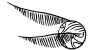
\includegraphics[scale=0.4]{boccino.png}
\centering
\end{figure}

Harry aveva ora acquistato gli ingredienti per le pozioni e il calderone, e, oh, un paio di accessori. Oggetti che sembravano le cose giuste da portare nella Borsa Conservante di Harry (alias Moke Super Pouch \textsc{qx}31 con Incantesimo dell’Estensione Impercettibile, Incantesimo di Recupero e Bordo Allargante). Acquisti intelligenti e sensati.

Harry sinceramente non capiva perché la professoressa McGonagall sembrasse così \textit{sospettosa}.

In quel momento, Harry era in un negozio abbastanza costoso da essere posto lungo la tortuosa strada principale di Diagon Alley. Il negozio aveva una parte anteriore aperta, con la merce disposta su scaffalature di legno inclinate, e protetta solo da tenui bagliori grigi e da una commessa giovanile in una versione molto ridotta delle vesti da strega, che mostrava ginocchia e gomiti.

Harry stava esaminando l’equivalente magico di un kit di pronto soccorso, il Pacchetto Extra di Guarigione di Emergenza. C’erano due lacci emostatici auto-serranti. Una Pozione di Stabilizzazione, che avrebbe rallentato la perdita di sangue e prevenuto il trauma. Una siringa di quello che sembrava fuoco liquido, che avrebbe dovuto ridurre drasticamente la circolazione nella zona trattata, mantenendo al contempo l’ossigenazione del sangue per un massimo di tre minuti, se fosse stato necessario evitare che un veleno si diffondesse attraverso il corpo. Un panno bianco che poteva essere avvolto su di una parte del corpo per renderla temporaneamente insensibile al dolore. Più un numero imprecisato di altri gingilli che Harry era stato totalmente incapace di comprendere, come il «Trattamento contro l’Esposizione a un Dissennatore», che aveva l’aspetto e l’odore del normale cioccolato. Oppure l’«Antidoto per Confondimorso», che sembrava un piccolo uovo vibrante ed era accompagnato da un cartellino che mostrava come incastrarlo su per la narice di qualcuno.

«Per cinque galeoni è un acquisto certo, non è d’accordo?» chiese alla professoressa McGonagall, e la commessa adolescente che si librava là vicino annuì con entusiasmo.

Harry si era aspettato che la professoressa gli indirizzasse una qualche sorta di commento di approvazione a proposito della sua prudenza e preparazione.

Ciò che invece stava ricevendo poteva essere descritto solo come il Malocchio.

«Ed esattamente \textit{per quale motivo}», chiese la professoressa McGonagall con forte scetticismo, «si aspetta di \textit{aver bisogno} di un kit di guarigione, giovanotto?» (Dopo lo sfortunato incidente al negozio di Pozioni, la professoressa McGonagall stava cercando di evitare di dire «signor Potter», se qualcuno era nelle vicinanze.)

La bocca di Harry si aprì e si richiuse. «Non mi \textit{aspetto} di averne bisogno! È solo nell’eventualità!»

«Solo nell’eventualità di \textit{che cosa?}»

Harry spalancò gli occhi. «Lei pensa che stia \textit{progettando} di fare qualcosa di pericoloso ed è \textit{per questo} che voglio un kit medico?»

Uno sguardo di torvo sospetto e d’ironica incredulità fu la risposta.

«Grande Giove!» disse Harry. (Quella era un’espressione che aveva imparato dalla scienziato pazzo Doc Brown di \textit{Ritorno al futuro}). «Lo stava pensando anche quando ho comprato la Pozione Caduta-Piuma, l’Algabranchia, e le Pillole del Cibo e dell’Acqua?»

«Sì.»

Harry scosse la testa per lo stupore. «E che genere di piano pensa che stia \textit{tramando}, ora?»

«Non lo so», disse la professoressa McGonagall cupamente, «ma finisce con lei che consegna una tonnellata di argento a Gringotts, o nella conquista del mondo.»

«Conquista del mondo è una frase così brutta. Preferisco chiamarla ottimizzazione del mondo.»

Questa battuta esilarante non riuscì a tranquillizzare la strega, che stava rivolgendogli lo Sguardo del Fato.

«Uau», disse Harry, quando si rese conto che era seria. «Lo pensa davvero. Pensa davvero che stia progettando di fare qualcosa di pericoloso.»

«Sì.»

«Come se questo fosse \textit{l’unico} motivo per comprare un kit di pronto soccorso? Non la prenda male, professoressa McGonagall, ma \textit{con che razza di bambini folli è abituata a trattare?}»

«Grifondoro» esclamò la professoressa McGonagall, e la parola portò con sé un carico di amarezza e disperazione che ricadde come una maledizione eterna su ogni entusiasmo e buon umore giovanile.

«Vicepreside professoressa Minerva McGonagall», disse Harry, mettendo le mani sui fianchi in un atteggiamento severo. «Non ho intenzione di andare in Grifondoro –»

A questo punto la Vicepreside s’intromise dicendo qualcosa del tipo che se quello \textit{l’avesse fatto}, ella avrebbe scoperto come uccidere un cappello, una strana osservazione che Harry lasciò passare senza commenti, anche se la commessa sembrò avere un attacco di tosse improvvisa.

«– ho intenzione di andare in Corvonero. E se davvero pensa che stia progettando di fare qualcosa di pericoloso, allora, onestamente, non mi ha capito per \textit{niente}. Non mi \textit{piace} il pericolo, è \textit{spaventoso}. Sono \textit{prudente}. Sono \textit{cauto}. Mi sto preparando per \textit{eventualità impreviste}. Come i miei genitori cantavano per me: \textit{Siate pronti! Questa è la canzone di marcia dei Boy Scout! Siate pronti! Mentre marciate attraverso la vita! Non siate nervosi, non siate agitati, non siate timorosi — siate pronti!}»

(I genitori di Harry gli avevano cantato in effetti sempre e solo quei versi in particolare della canzone di Tom Lehrer, e Harry era beatamente inconsapevole di tutto il resto.)

La posizione della professoressa McGonagall si ammorbidì leggermente – anche se per lo più ciò avvenne quando Harry disse che era destinato a Corvonero. «Per che genere di \textit{eventualità} immagina che questo kit potrebbe \textit{prepararla}, giovanotto?»

«Una delle mie compagne di classe viene morsa da un mostro orribile, e mentre rovisto freneticamente nella mia borsa mokeskin in cerca di qualcosa che potrebbe aiutarla, lei mi guarda tristemente e con il suo ultimo respiro dice, ‘\textit{Perché non eri preparato?}’ E poi muore, e mentre i suoi occhi si chiudono so che non mi perdonerà mai –»

Harry udì gemere la commessa, e alzò lo sguardo per vederla mentre lo fissava con le labbra serrate. Poi la giovane donna si voltò e fuggì nei recessi più profondi del negozio.

\textit{Che cosa…?}

La professoressa McGonagall si chinò e prese la mano di Harry tra le proprie, delicatamente ma con fermezza, e tirò Harry fuori dalla strada principale di Diagon Alley, portandolo in un vicolo tra due negozi che era pavimentato in mattoni sporchi e terminava in un muro di solida terra nera.

L’alta strega puntò la bacchetta verso la strada principale e parlò, «\textit{Quietus}» disse, e uno schermo di silenzio scese intorno a loro, bloccando tutti i rumori della strada.

\textit{Che cosa ho fatto di sbagliato…}

La professoressa McGonagall si voltò a osservare Harry. Non aveva la completa Espressione da Rimprovero da adulto, ma la sua espressione era piatta, controllata. «Deve ricordare, signor Potter», disse, «che c’è stata una guerra in questo Paese non più di dieci anni fa. Tutti hanno perso qualcuno, e parlare di amici che muoiono tra le tue braccia — non va fatto con leggerezza.»

«Io — io non volevo –» L’implicazione cadde come un sasso nell’immaginazione eccezionalmente vivida di Harry. Aveva parlato di qualcuno che esalava il suo ultimo respiro — e poi la commessa era fuggita — e la guerra era finita dieci anni prima, quindi la ragazza avrebbe avuto al massimo di otto o nove anni, quando, quando, «Mi dispiace, io non volevo…» Harry si sentì soffocare, e si voltò per sfuggire allo sguardo dell’anziana strega, ma c’era un muro di terra che bloccava la sua strada e non aveva ancora la sua bacchetta. «Mi dispiace, mi dispiace, mi \textit{dispiace!}»

Ci fu un profondo sospiro alle sue spalle. «So che è così, signor Potter.»

Harry osò sbirciare dietro di sé. La professoressa McGonagall sembrava solo triste, ora. «Mi dispiace», disse Harry di nuovo, sentendosi miserabile. «Qualcosa di simile è accaduto a –» e poi Harry chiuse le labbra e mise una mano sulla bocca per sicurezza.

Il viso dell’anziana strega divenne un po’ più triste. «Deve imparare a pensare prima di parlare, signor Potter, oppure passerà la sua vita senza molti amici. Questo è stato il destino di molti Corvonero, e spero che non sia il suo.»

Harry voleva solo fuggire via. Voleva tirar fuori una bacchetta e cancellare l’intera faccenda dalla memoria della professoressa McGonagall, tornare con lei nuovamente fuori dal negozio, \textit{e fare in modo che non fosse mai accaduto} –

«Ma per rispondere alla sua domanda, signor Potter, no, niente \textit{del genere} è mai successo a me. Certo, ho visto un amico esalare il suo ultimo respiro, una o sette volte. Ma nessuno di loro mi ha mai maledetto mentre moriva, e non ho mai pensato che non mi avrebbe perdonato. Perché lei dovrebbe \textit{dire} una cosa del genere, signor Potter? Perché dovrebbe persino pensarla?»

«Io, io, io», Harry deglutì. «È solo che cerco sempre di immaginare la cosa peggiore che potrebbe accadere», e forse aveva anche scherzato un po’, ma avrebbe preferito mordersi la lingua piuttosto che dirlo ora.

«Che cosa?» disse la professoressa McGonagall. «Ma \textit{perché?}»

«Così posso impedire che accada!»

«Signor Potter…» la voce della vecchia strega si affievolì. Poi sospirò, e si inginocchiò accanto a lui. «Signor Potter», disse ora con dolcezza, «non è responsabilità sua prendersi cura degli studenti di Hogwarts. È mia. Non lascerò che accada nulla di male a lei o a chiunque altro. Hogwarts è il posto più sicuro per i maghi bambini in tutto il mondo della stregoneria, e Madam Pomfrey ha un’intera infermeria per le guarigioni. Non avrà affatto bisogno del kit di guarigione, figuriamoci di uno da cinque galeoni.»

«Invece \textit{sì!}» proruppe Harry. «\textit{Nessun luogo} è perfettamente sicuro! E se i miei genitori avessero un attacco di cuore o fossero coinvolti in un incidente quando tornerò a casa per Natale – Madam Pomfrey non sarà lì, avrò bisogno di un kit di guarigione tutto mio –»

«Ma in nome di Merlino, \textit{cosa…}» disse la professoressa McGonagall. Si alzò e guardò giù verso Harry, con un’espressione divisa tra il fastidio e la preoccupazione. «Non c’è bisogno di pensare a queste cose terribili, signor Potter!»

L’espressione di Harry si contorse diventando amarezza, a sentire quelle parole. «\textit{Sì} che c’è! Se non ci pensa, non solo si farà male, finirà per fare male ad altre persone!»

La professoressa McGonagall aprì la bocca, poi la richiuse. La strega si massaggiò la radice del naso, l’espressione pensierosa. «Signor Potter… se dovessi offrirle di stare ad ascoltarla per un po’… ci sarebbe qualcosa che desidererebbe raccontarmi?»

«A proposito di cosa?»

«A proposito del perché lei sia convinto di dover stare sempre in guardia contro le cose terribili che potrebbero accaderle.»

Harry la guardò perplesso. Si trattava di un assioma auto-evidente. «Beh…» iniziò Harry lentamente. Cercò di organizzare i pensieri. Come \textit{poteva} spiegarsi con una professoressa-strega, quando ella non conosceva neppure le basi? «Ricercatori babbani hanno scoperto che le persone sono sempre molto ottimiste, rispetto alla realtà. Del tipo, dicono che ci vorranno due giorni per terminare qualcosa e ci vogliono dieci giorni, oppure dicono che ci vorranno due mesi e ci vogliono più di 35 anni. Ad esempio, in un esperimento hanno chiesto a degli studenti di stimare il tempo entro cui erano sicuri al 50\%, al 75\% e al 99\% di completare i loro compiti, e solo il 13\%, il 19\% e il 45\% degli studenti terminò entro quelle stime. E hanno scoperto che la ragione era che quando chiesero a un gruppo la stima per il caso migliore, quello in cui tutto andava nel migliore dei modi, e a un altro gruppo la stima del caso medio, quello in cui tutto andava come al solito, ottenevano risposte che erano statisticamente indistinguibili. Vede, se chiede a qualcuno ciò che si aspetta nel caso \textit{normale}, egli immaginerà quella che sembra la linea di massima probabilità a ciascun passo lungo il percorso — tutto va secondo i piani, senza sorprese. Ma effettivamente, dal momento che più della metà degli studenti non rispettò la scadenza che erano sicuri al 99\% di rispettare, la realtà offre solitamente risultati un po’ peggiori rispetto allo ‘scenario peggiore’. Si chiama errore di pianificazione, e il modo migliore per correggerlo è quello di chiedere quanto tempo c’è voluto l’ultima volta che si è provato. Questo si chiama usare il punto di vista esterno invece di quello interno. Ma quando stiamo per fare qualcosa di nuovo e non possiamo procedere in questo modo, dobbiamo semplicemente essere molto, molto, molto pessimisti. Come dire, così pessimisti che la realtà si dimostra effettivamente \textit{migliore} di quanto ci aspettavamo più o meno tanto spesso e con uguale intensità di quando si dimostra peggiore. In realtà è \textit{talmente difficile} essere così pessimisti, che c’è una possibilità decente di \textit{sottostimare} la vita reale. Come dire, faccio questo grande sforzo di essere pessimista e immagino che uno dei miei compagni di classe venga morso, ma quello che succede in realtà è che i Mangiamorte sopravvissuti attaccano tutta la scuola per arrivare a me. Ma da un punto di vista più allegro –»

«Si fermi», disse la professoressa McGonagall.

Harry si fermò. Era appena stato sul punto di sottolineare che almeno sapeva che il Signore Oscuro non avrebbe attaccato, in quanto era morto.

«Penso di non essermi spiegata abbastanza chiaramente», disse la strega, il suo nitido accento scozzese che sembrò ancora più attento. «È successo qualcosa a \textit{lei personalmente} che l’ha spaventata, signor Potter?»

«Quello che è successo a me personalmente è solo una prova aneddotica», spiegò Harry. «Non ha lo stesso peso di un articolo scientifico replicato e revisionato a proposito di uno studio controllato con assegnazione casuale, molti soggetti, ampia \textit{effect size} e forte significatività statistica.»

La professoressa McGonagall strinse con le dita la radice del naso, inspirò e espirò. «Vorrei saperlo comunque», disse.

«Uhm…» iniziò Harry. Fece un respiro profondo. «C’erano stati alcuni scippi nel nostro quartiere, e mia madre mi chiese di restituire un tegame che aveva preso in prestito da una vicina a due strade di distanza, e risposi che non volevo, perché avrebbero potuto aggredirmi, e lei mi disse, ‘Harry, non dire cose del genere!’ Come se pensarci lo \textit{facesse} succedere, dunque se non ne avessi parlato, sarei stato al sicuro. Cercai di spiegare perché non ne ero rassicurato, e lei mi fece portare la pentola comunque. Ero troppo giovane per sapere quanto fosse statisticamente improbabile che uno scippatore mi scegliesse come vittima, ma ero abbastanza grande da sapere che non pensare a qualcosa non impedisce che accada, quindi ero davvero spaventato.»

«Nient’altro?», chiese la professoressa McGonagall dopo una pausa, quando divenne chiaro che Harry aveva finito. «Non c’è niente \textit{altro} che le è successo?»

«So che non \textit{sembra} gran che», si difese Harry. «Ma fu uno di quei momenti cruciali di una vita, sa? Voglio dire, \textit{sapevo} che non pensare a qualcosa non impediva che accadesse, lo \textit{sapevo}, ma mi resi conto che la mamma la pensava davvero in quel modo.» Harry si fermò, alle prese con la rabbia che stava iniziando a rimontare ora che ci ripensava. «\textit{Non mi voleva ascoltare}. Cercai di dirglielo, la pregai di non farmi uscire, e lei \textit{la mise sul ridere}. Tutto ciò che dicevo, lei lo considerava come una specie di scherzo…» Harry costrinse la rabbia nera a ritirarsi nuovamente. «In quel momento mi resi conto che tutti quelli che avrebbero dovuto proteggermi erano in realtà folli, e che non mi avrebbero ascoltato, non importava quanto li pregassi, e che non avrei potuto mai fare affidamento su di loro per fare qualcosa nel modo giusto.» A volte non era sufficiente essere bene intenzionati, a volte si doveva essere sani di mente…

Ci fu un lungo silenzio.

Harry si prese il tempo per respirare profondamente e calmarsi. Non c’era motivo di arrabbiarsi. Non c’era motivo di arrabbiarsi. \textit{Tutti} i genitori erano così, \textit{nessun} adulto si sarebbe abbassato abbastanza da mettersi sullo stesso piano di un bambino e ascoltarlo, i suoi genitori genetici non sarebbero stati diversi. La sanità mentale era una piccola scintilla nella notte, un’eccezione infinitamente rara alla regola della follia, quindi non c’era motivo di arrabbiarsi.

Harry non si piaceva quando era arrabbiato.

«Grazie per averlo condiviso, signor Potter», disse la professoressa McGonagall dopo un po’. C’era un’espressione distratta sul suo viso (quasi esattamente la stessa espressione che era apparsa sul volto di Harry durante l’esperimento con la borsa, se solo Harry si fosse visto in uno specchio). «Dovrò rifletterci.» Si voltò verso l’imbocco del vicolo, e alzò la bacchetta –

«Uhm» disse Harry, «possiamo andare a prendere il kit di guarigione, ora?»

La strega si fermò e lo guardò fermamente. «E se dicessi di no — che è troppo costoso e non ne avrà bisogno — allora che succederebbe?»

L’espressione di Harry si contorse diventando amara. «Esattamente quello che sta pensando, professoressa McGonagall. \textit{Esattamente} quello che sta pensando. Concluderei che lei è un altro folle adulto al quale non posso parlare, e comincerei a progettare un piano per mettere comunque le mani sul kit di guarigione.»

«Sono il suo tutore in questo viaggio», disse la professoressa McGonagall con una sfumatura di pericolosità. «\textit{Non le permetterò} di menarmi per il naso.»

«Capisco», disse Harry. Tenne il risentimento fuori dalla sua voce, e non disse nessuna delle altre cose che gli erano venute in mente. La professoressa McGonagall gli aveva detto di pensare prima di parlare. Probabilmente non se lo sarebbe ricordato domani, ma poteva almeno ricordarlo per cinque minuti.

La bacchetta nella mano della strega disegnò una forma circolare, e i rumori di Diagon Alley tornarono. «Bene, giovanotto», disse. «Andiamo a prendere quel kit di guarigione.»

Harry rimase a bocca aperta per la sorpresa. Poi si affrettò dietro di lei, quasi inciampando nella sua corsa improvvisa.

\begin{figure}[h]
	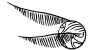
\includegraphics[scale=0.4]{boccino.png}
	\centering
\end{figure}

Il negozio era come l’avevano lasciato, articoli riconoscibili e irriconoscibili ancora disposti sull’espositore di legno inclinato, il bagliore grigio ancora a proteggerli e la commessa tornata alla sua postazione. La ragazza alzò lo sguardo mentre si avvicinavano, e il suo viso ne mostrò la sorpresa.

«Mi dispiace», disse lei mentre si fecero più vicini, e Harry parlò quasi nello stesso momento, «Chiedo scusa per –»

Si interruppero e si guardarono l’un l’altra, e poi la commessa rise un po’. «Non avevo intenzione di metterti nei guai con la professoressa McGonagall», disse lei. La sua voce si abbassò in maniera cospiratoria. «Spero che non sia stata troppo terribile con te.»

«\textit{Della!}» scattò la professoressa McGonagall, l’espressione scandalizzata.

«Sacchetto d’oro», disse Harry alla sua borsa, e poi tornò a guardare la commessa mentre contava cinque galeoni. «Non ti preoccupare, ho capito che è terribile con me solo perché mi vuole bene.»

Contò i cinque galeoni alla commessa, mentre la professoressa McGonagall stava farfugliando qualcosa di poco importante. «Un Pacchetto Extra di Guarigione di Emergenza, per favore.»

Era davvero piuttosto inquietante vedere come il Bordo Allargante ingoiasse il kit medico delle dimensioni di una valigetta. Harry non poté fare a meno di chiedersi cosa sarebbe successo se avesse cercato di entrare egli stesso nella borsa mokeskin, dato che solo la persona che aveva messo dentro qualcosa sarebbe dovuta essere in grado di riprenderla.

Quando la borsa ebbe finito di… mangiare… il suo acquisto conquistato con molta fatica, Harry poté giurare di averle sentito fare un ruttino. Quello \textit{doveva} essere stato inserito volutamente. L’ipotesi alternativa era troppo orribile da contemplare… infatti Harry non riusciva nemmeno a pensare a qualunque ipotesi alternativa. Tornò a guardare la professoressa, mentre ripresero a passeggiare per Diagon Alley ancora una volta. «Dove si va?»

La professoressa McGonagall indicò un negozio che sembrava fosse stato costruito con della carne, invece che con i mattoni, e rivestito di pelliccia, invece che di pittura. «Gli animali domestici di piccola taglia sono ammessi a Hogwarts — potrebbe prendere un gufo per inviare le lettere, per esempio –»

«Posso pagare uno zellino o qualcosa del genere e \textit{affittare} un gufo quando ho bisogno di spedire la posta?»

«Sì», disse la professoressa McGonagall.

«Allora credo enfaticamente di \textit{no.}»

La professoressa McGonagall annuì, come se stesse spuntando un elemento di una lista. «Posso chiedere perché no?»

«Ho avuto una pietra domestica, una volta. È morta.»

«Non pensa di essere in grado di avere cura di un animale domestico?»

«\textit{Potrei}», disse Harry, «ma finirei per ossessionarmi tutto il tempo chiedendomi se mi fossi ricordato di nutrirlo, quel giorno, o se stesse lentamente morendo di fame nella sua gabbia, chiedendosi dove sia il suo padrone e perché non ci sia del cibo.»

«Povero gufo» disse l’anziana strega con voce dolce. «Abbandonato così. Mi chiedo che cosa farebbe.»

«Beh, mi aspetterei che avesse veramente fame e iniziasse a provare a uscire dalla gabbia o dalla scatola o da qualsiasi altra cosa, anche se probabilmente non avrebbe molta fortuna –» Harry si fermò di colpo.

La strega continuò, ancora con quella voce morbida. «E che cosa gli accadrebbe dopo?»

«Mi scusi» disse Harry, e afferrò la mano della professoressa McGonagall, delicatamente ma con fermezza, e la condusse in un altro vicolo; dopo aver schivato tanti ammiratori, quella precauzione era diventata quasi automatica. «La prego, lanci l’incantesimo del silenzio.»

«\textit{Quietus.}»

La voce di Harry stava tremando. «Quel gufo \textit{non} rappresenta me, i miei genitori non mi hanno mai chiuso in uno stanzino a morire di fame, \textit{non ho} paura di essere abbandonato e \textit{non mi piace la direzione che i suoi pensieri hanno preso, professoressa McGonagall!}»

La strega lo guardò seriamente. «E che pensieri sarebbero, signor Potter?»

«Lei pensa che io abbia» Harry ebbe dei problemi a dirlo, «che abbia subito degli \textit{abusi?}»

«Li ha subiti?»

«\textit{No!}» gridò Harry. «No, mai! Pensa che sia \textit{stupido?} Conosco il concetto di abuso su minori, so cosa significa toccare in maniera inappropriata e tutto il resto e se qualcosa di simile fosse capitato avrei chiamato la polizia! E l’avrei segnalato al dirigente scolastico! E avrei cercato i servizi sociali sull’elenco del telefono! E l’avrei detto al Nonno e alla Nonna e alla signora Figg! Ma i miei genitori non hanno \textit{mai} fatto niente di simile, mai mai \textit{mai!} Come \textit{osa} insinuare una cosa del genere!»

L’anziana strega lo guardò con fermezza. «È mio dovere di Vicepreside indagare possibili segni di abusi nei bambini affidati alle mie cure.»

La rabbia di Harry stava crescendo fuori controllo, trasformandosi in una furia pura e assoluta. «Non si \textit{azzardi} mai a riferire una sola parola di queste, queste \textit{insinuazioni} a nessun’altro! \textit{Nessuno}, mi ha capito, McGonagall? Un’accusa simile può rovinare le persone e distruggere le famiglie, anche quando i genitori sono completamente innocenti! Ho letto di casi simili sui giornali!» La voce di Harry stava salendo a un grido acuto. «Il \textit{sistema} non sa come \textit{fermarsi}, non crede ai genitori \textit{né} ai figli quando dicono che non è successo niente! \textit{Non si azzardi a minacciare la mia famiglia con questa storia! Non le lascerò distruggere casa mia!}»

«Harry», disse dolcemente la vecchia strega, e allungò una mano verso di lui –

Harry fece un brusco passo indietro, e la sua mano si alzò di scatto e allontanò quella di lei.

McGonagall si immobilizzò, poi ritirò la mano e fece un passo indietro. «Harry, va tutto bene», disse. «Ti credo.»

«\textit{Davvero}», sibilò Harry. La furia ruggiva ancora nel suo sangue. «O sta solo aspettando di allontanarsi da me in modo da poter compilare i documenti?»

«Harry, ho visto la tua casa. Ti ho visto con i tuoi genitori. Ti amano. Tu li ami. Ti credo quando dici che i tuoi genitori non stanno abusando di te. Ma ho \textit{dovuto} chiedere, perché c’è qualcosa che non quadra.»

Harry la guardò con freddezza. «Del tipo?»

«Harry, ho visto molti bambini maltrattati durante la mia permanenza a Hogwarts, ti spezzerebbe il cuore sapere quanti. E, quando sei felice, non ti comporti come uno di quei bambini, per \textit{niente}. Sorridi agli sconosciuti, abbracci le persone, ti ho messo la mano sulla spalla e non hai battuto ciglio. Ma a volte, solo a volte, dici o fai qualcosa che sembra \textit{molto} simile… a quello che farebbe qualcuno che ha trascorso i suoi primi undici anni chiuso in una cantina. Non nella famiglia amorevole che ho conosciuto.» La professoressa McGonagall inclinò la testa, la sua espressione divenne ancora una volta perplessa.

Harry prese quelle parole e le elaborò. La rabbia nera cominciò a defluire, mentre si rendeva conto che era ascoltato con rispetto, e che la sua famiglia non era in pericolo.

«E come \textit{spiega} le sue osservazioni, professoressa McGonagall?»

«Non lo so», disse lei. «Ma è possibile che le sia accaduto qualcosa che non ricorda.»

La furia esplose nuovamente in Harry. Sembrava tutto troppo simile a quello che aveva letto nei resoconti dei giornali sulle famiglie spezzate. «La soppressione della memoria è \textit{pseudoscienza!} La gente \textit{non reprime} i ricordi traumatici, se li ricorda fin \textit{troppo} bene per il resto della sua vita!»

«No, signor Potter. C’è un Incantesimo chiamato Obliazione.»

Harry si bloccò sul posto. «Un incantesimo che cancella i ricordi?»

L’anziana strega annuì. «Ma non tutte le conseguenze di quell’esperienza, se capisce quello che intendo, signor Potter».

Un brivido scese lungo la schiena di Harry. \textit{Quella} ipotesi… \textit{non poteva} essere facilmente confutata. «Ma i miei genitori non possono farlo!»

«In effetti no», concesse la professoressa McGonagall. «Ci sarebbe voluto qualcuno del mondo dei maghi. Non c’è… non c’è modo di esserne certi, temo.»

Le capacità razionaliste di Harry presero a funzionare nuovamente. «Professoressa McGonagall, quanto è certa delle sue osservazioni, e quali spiegazioni alternative potrebbero anche esserci?»

La strega aprì le mani, come per mostrare che erano vuote. «Sicura? Sono sicura di \textit{niente}, signor Potter. In tutta la mia vita non ho mai incontrato qualcuno come lei. A volte non sembra un undicenne e neppure tanto \textit{umano}.»

Le sopracciglia di Harry salirono verso il cielo –

«Mi dispiace!» la professoressa McGonagall disse in fretta. «Mi dispiace molto, signor Potter. Stavo cercando fare un discorso e ho paura che sia venuto fuori diverso da quello che avevo in mente –»

«Al contrario, professoressa McGonagall», disse Harry, e sorrise lentamente. «Lo prendo come un grandissimo complimento. Ma le dispiacerebbe se le offrissi una spiegazione alternativa?»

«Prego.»

«I bambini non sono fatti per essere troppo più intelligenti dei loro genitori», disse Harry. «O troppo più sani di mente, forse — mio padre potrebbe probabilmente superarmi in arguzia se lui, sa, \textit{provasse} a farlo, invece di usare la sua intelligenza da adulto principalmente per scovare nuove ragioni per non cambiare idea –» Harry si fermò. «Sono troppo intelligente, Professoressa. Non ho nulla da dire ai bambini normali. Gli adulti non mi rispettano a sufficienza per parlare veramente con me. E, francamente, anche se lo facessero, non sembrerebbero intelligenti come Richard Feynman, quindi tanto vale leggere qualcosa che Richard Feynman ha scritto, invece. Sono \textit{isolato}, professoressa McGonagall. Sono stato isolato per tutta la mia vita. Forse questo ha alcuni degli stessi effetti del rimanere rinchiuso in una cantina. E sono troppo intelligente per guardare ai miei genitori nel modo in cui i bambini sono progettati per fare. I miei genitori mi amano, ma non si sentono obbligati a rispondere alla ragione, e qualche volta mi sento come se loro fossero i bambini — bambini che \textit{non vogliono ascoltare} e che hanno un’autorità assoluta su tutta la mia esistenza. Cerco di non essere troppo amareggiato per questo, ma cerco anche di essere onesto con me stesso, quindi, sì, sono amareggiato. E ho anche un problema di gestione della rabbia, ma ci sto lavorando. Questo è tutto.»

«\textit{Questo è tutto?}»

Harry annuì con decisione. «Questo è tutto. Sicuramente, professoressa McGonagall, anche nella Gran Bretagna magica, la spiegazione normale è sempre degna di essere \textit{considerata}, no?»

\begin{figure}[h]
	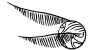
\includegraphics[scale=0.4]{boccino.png}
	\centering
\end{figure}

Più tardi, quello stesso giorno, il sole stava scendendo nel cielo estivo e gli acquirenti cominciavano a scemare via dalle strade. Alcuni negozi avevano già chiuso; Harry e la professoressa McGonagall avevano comprato i suoi libri di testo da Flourish and Blotts appena prima del termine. Con appena una leggera esplosione quando Harry era andato dritto verso la sezione «Aritmanzia» e aveva scoperto che i libri di testo del settimo anno non richiedevano niente di più matematicamente avanzato della trigonometria.

In quel momento, però, i sogni di cogliere i risultati più facili della ricerca erano lontani dalla mente di Harry.

In quel momento, essi stavano uscendo da Ollivander’s, e Harry stava fissando la propria bacchetta. L’agitò, e produsse scintille multicolori, cosa che in realtà non avrebbe dovuto essere così sconvolgente dopo tutto quello che aveva già visto, ma in qualche modo –

\textit{Posso compiere magie.}

\textit{Io. Voglio dire, io personalmente. Sono una creatura magica; sono un mago.}

Aveva \textit{sentito} la magia scorrere su per il suo braccio, e in quell’istante aveva realizzato che aveva sempre avuto quella sensazione, che l’aveva posseduto tutta la vita, quel senso che non era vista, udito, olfatto, gusto o tatto, ma semplicemente magia. Come avere gli occhi ma tenerli sempre chiusi, così da non accorgersi neppure di vedere l’oscurità; e poi un giorno gli occhi si aprivano e vedevano il mondo. Lo sconvolgimento si era riversato attraverso di lui, toccando parti del suo sé, svegliandole, e poi si era andato a spegnere nel giro di pochi secondi; lasciando solo la conoscenza certa che ora era un mago, e lo era sempre stato, e persino che, in qualche modo particolare, l’aveva sempre saputo.

E –

«\textit{È davvero curioso che lei fosse predestinato a questa bacchetta quando la sua gemella, beh, la sua gemella le ha procurato quella cicatrice.}»

Non era possibile che fosse una coincidenza. C’erano state \textit{migliaia} di bacchette in quel negozio. Beh, va bene, in effetti \textit{poteva} essere una coincidenza, c’erano sei miliardi di persone nel mondo e coincidenze del tipo una-su-mille si avveravano ogni giorno. Ma il Teorema di Bayes diceva che ogni ipotesi ragionevole che rendesse \textit{più} probabile di mille a uno che egli entrasse in possesso della bacchetta gemella di quella del Signore Oscuro era avvantaggiata.

La professoressa McGonagall aveva semplicemente detto \textit{molto peculiare} e l’aveva finita lì, cosa che aveva sconvolto Harry per la pura e preponderante \textit{mancanza di curiosità} dei maghi e delle streghe. In nessun mondo \textit{concepibile} Harry avrebbe semplicemente fatto «Uhm» e se ne sarebbe uscito dal negozio senza neppure \textit{provare} a formulare un’ipotesi per ciò che stava accadendo.

La sua mano sinistra andò a toccare la sua cicatrice.

Cosa… \textit{esattamente…}

«Ora è un mago completo», disse la professoressa McGonagall. «Congratulazioni.»

Harry annuì.

«E cosa pensa del mondo dei maghi?»

«È strano», disse Harry. «Dovrei pensare a tutto ciò che ho visto della magia… a tutto ciò che ora so essere possibile, e a tutto ciò che ora so essere una bugia, e tutto il lavoro davanti a me per comprenderlo. Eppure mi trovo distratto da banalità relative come», Harry abbassò la voce, «la faccenda del Ragazzo-Che-È-Sopravvissuto.» Non sembrava ci fosse nessuno vicino, ma era inutile tentare il destino.

La professoressa McGonagall si schiarì la voce. «Davvero? Sono sorpresa.»

Harry annuì. «Sì. È semplicemente… \textit{strano}. Scoprire di essere stato parte di questa grande storia, l’impresa di sconfiggere il grande e terribile Signore Oscuro, e che è già \textit{finita}. Completata. Definitivamente terminata. È come essere Frodo Baggins e scoprire che i tuoi genitori ti hanno portato a Monte Fato e ti hanno fatto gettare l’Anello quando avevi solo un anno, e non ti ricordi niente.»

Il sorriso della professoressa McGonagall era diventato piuttosto fisso.

«Sa, se fossi chiunque altro, qualunque altra persona, probabilmente sarei preoccupato di essere all’altezza di quell’inizio. \textit{Mio dio, Harry, cos’hai fatto da quando hai sconfitto il Signore Oscuro? Hai aperto una tua libreria? Che bella idea! Ehi, lo sapevi che ho dato il tuo nome a mio figlio?} Ma conto sul fatto che questo non sarà un problema.» Harry sospirò. «Ad ogni modo… è quasi sufficiente a farmi sperare che vi siano alcune questioni in sospeso in questa impresa, giusto in modo che possa dire di avervi realmente, sa, \textit{partecipato} in qualche modo.»

«Oh?» disse la professoressa McGonagall in un tono strano. «Che cosa ha in mente?»

«Beh, per esempio, lei ha menzionato il fatto che i miei genitori sono stati traditi. Chi li ha traditi?»

«Sirius Black», disse la strega, quasi sibilando il nome. «È ad Azkaban. La prigione dei maghi.»

«Quanto è probabile che quel Sirius Black fugga dalla prigione e io debba inseguirlo e sconfiggerlo in una qualche sorta di duello spettacolare, o meglio ancora mettere una grossa taglia sulla sua testa e nascondermi in Australia mentre attendo i risultati?»

La professoressa McGonagall sbatté le palpebre. Due volte. «Improbabile. Nessuno è mai fuggito da Azkaban, e dubito che \textit{lui} sarà il primo.»

Harry era un po’ scettico riguardo quel «\textit{nessuno} è \textit{mai} fuggito da Azkaban». Eppure, forse con la magia era possibile ottenere una prigione perfetta fino a quasi il 100\%, specie se tu avevi una bacchetta e loro no. Il modo migliore per uscire sarebbe stato quello di non andarci, tanto per cominciare.

«Va bene, allora», disse Harry. «Sembra che tutto sia stato terminato alla perfezione.» Sospirò, strofinandosi la testa col palmo. «O forse il Signore Oscuro non morì \textit{davvero} quella notte. Non completamente. Il suo spirito si trattiene, sussurrando alle persone in incubi che sbiadiscono dopo il risveglio, cercando un modo di tornare alle terre dei vivi che ha giurato di distruggere, e ora, in accordo con un’antica profezia, lui e io siamo serrati in un duello mortale in cui il vincitore perderà e lo sconfitto vincerà –»

La testa della professoressa McGonagall ruotò, e i suoi occhi guizzarono intorno, come se scandagliasse la strada in cerca di ascoltatori.

«Sto \textit{scherzando}, professoressa», disse Harry con un certo fastidio. Cavolo, perché prendeva sempre tutto così seriamente –

Una sensazione di profonda ansia nacque alla bocca dello stomaco di Harry.

La professoressa McGonagall osservò Harry con un’espressione calma. Un’espressione molto, \textit{molto} calma. Poi mise su un sorriso. «Naturalmente, signor Potter.»

\textit{Oh cavolo.}

Se Harry avesse avuto bisogno di formalizzare la deduzione non verbale che era appena sorta nella sua mente, se ne sarebbe dovuto uscire con qualcosa tipo ‘se stimassi che la probabilità che la professoressa McGonagall faccia ciò che ho appena visto come risultato dell’attento controllo di sé stessa, contro la distribuzione di probabilità di tutte le cose che farebbe \textit{naturalmente} se facessi una pessima battuta, allora questo comportamento è una prova significativa del fatto che sta nascondendo qualcosa’.

Ma ciò che Harry pensò effettivamente fu, \textit{Oh cavolo.}

Harry girò la testa per scandagliare la strada. No, nessuno vicino. «\textit{Non è} morto, giusto?», sospirò Harry.

«Signor Potter –»

«Il Signore Oscuro è vivo. \textit{Ovviamente} è vivo. È stato un \textit{atto} di completo \textit{ottimismo} da parte mia aver persino sognato che non lo fosse. \textit{Devo} aver abbandonato il mio \textit{buon senso}, non riesco a \textit{immaginare} a cosa stavo \textit{pensando}. Solo perché \textit{qualcuno} ha detto che il suo corpo è stato trovato ridotto a un \textit{carbone}, non posso immaginare perché io abbia pensato che fosse \textit{morto. È chiaro} che ho ancora molto da imparare dell’arte del corretto \textit{pessimismo.}»

«Signor Potter –»

«Almeno mi dica che non c’è davvero una profezia…» La professoressa McGonagall gli stava ancora rivolgendo quel sorriso brillante e fisso. «Oh, lei mi sta \textit{certamente} prendendo in giro.»

«Signor Potter, non deve inventarsi cose di cui preoccuparsi –»

«Mi sta \textit{davvero} dicendo \textit{questo?} Immagini la mia reazione dopo, quando scoprissi che c’era davvero qualcosa di cui preoccuparsi.»

Il suo sorriso fisso vacillò.

Le spalle di Harry si ingobbirono. «Ho l’intero mondo della magia da studiare. \textit{Non ho tempo} per questo.»

Poi entrambi si zittirono, appena un uomo in fluenti vesti arancioni apparve sulla strada e lentamente li superò; gli occhi della professoressa McGonagall lo seguirono, discretamente. La bocca di Harry si muoveva mentre masticava con forza il proprio labbro, e qualcuno che avesse guardato da vicino avrebbe notato apparire una piccola macchia di sangue.

Quando l’uomo vestito di arancione si fu allontanato, Harry parlò di nuovo, in un basso mormorio. «Ha intenzione di dirmi la verità ora, professoressa McGonagall? E non si disturbi a minimizzare la questione, non sono stupido.»

«Lei ha solo \textit{undici anni}, signor Potter!» disse ella con un sussurro severo.

«E perciò subumano. Le chiedo scusa… per un momento l’avevo \textit{dimenticato}.»

«Si tratta di questioni terribili e importanti! Sono un \textit{segreto}, signor Potter! Si tratta di una \textit{catastrofe} che lei, che è ancora bambino, sappia anche solo questo! Non deve dirlo a \textit{nessuno}, ha capito? Assolutamente a nessuno!»

Come a volte accadeva quando Harry diventava \textit{sufficientemente} arrabbiato, il suo sangue si raffreddò, invece di scaldarsi, e una terribile e oscura chiarezza discese sulla sua mente, delineando le possibili tattiche e valutando le loro conseguenze con ferreo realismo.

\begin{itpars}
Fai notare che hai il diritto di sapere: fallimento. I bambini di undici anni non hanno diritto di sapere nulla, agli occhi della McGonagall.

Di’ che non sarete più amici: fallimento. Non tiene sufficientemente alla vostra amicizia.

Fai notare che sarai in pericolo se non sarai messo al corrente: fallimento. I piani sono già stati fatti sulla base della tua ignoranza. La scomodità certa di ripensarli sembrerà molto più sgradevole che la mera prospettiva incerta del tuo essere ferito.

Giustizia e ragione sono destinate entrambe a fallire. Devi trovare qualcosa che hai e che lei vuole, o qualcosa che tu puoi fare, e che lei teme…
\end{itpars}

Ah.

«Bene allora, Professoressa», disse Harry in una voce bassa e glaciale, «sembra che io abbia qualcosa che lei desidera. Lei può, se vuole, dirmi la verità, \textit{tutta} la verità, e in cambio manterrò i suoi segreti. O può cercare di tenermi all’oscuro in modo da usarmi come pedina, in tal caso non le dovrò nulla.»

McGonagall si fermò improvvisamente per strada. I suoi occhi divamparono e la sua voce eruppe in un sibilo. «Come osa!»

«\textit{Come osa lei!}» le sussurrò in risposta.

«Vorrebbe \textit{ricattarmi?}»

Le labbra di Harry si contorsero. «Le sto \textit{offrendo} un \textit{favore}. Le sto \textit{offrendo} la possibilità di proteggere il \textit{suo} prezioso segreto. Se rifiuta avrò \textit{ogni} legittimo motivo di domandare ad altri, non per ripicca contro di lei, ma perché \textit{devo sapere!} Superi la sua inutile rabbia contro un \textit{bambino} da cui si aspetta solo obbedienza, e comprenderà che ogni adulto sano di mente farebbe la stessa cosa! \textit{La guardi dalla mia prospettiva! Come si sentirebbe se \textsc{lei} fosse al mio posto?}»

Harry osservò McGonagall, notò il suo respiro pesante. Gli venne in mente che fosse il momento di allentare la pressione, di lasciarla cuocere a fuoco dolce per un po’. «Non deve decidere immediatamente», disse Harry in un tono più normale. «Capirei se volesse prendersi del tempo per pensare alla mia \textit{offerta}… ma l’avviso di una cosa», disse Harry con una voce che divenne più fredda. «Non provi a usare quell’incantesimo di Obliazione su di me. Qualche tempo fa ho elaborato una tecnica di segnalazione, e mi sono già mandato quel segnale. Se scoprissi quel segnale e non \textit{ricordassi} di essermelo mandato…» Harry lasciò che la propria voce si spegnesse in modo significativo.

Il volto di McGonagall lavorò, mentre le sue espressioni si scambiavano di posto. «Io… non stavo pensando di Obliarla, signor Potter… ma perché avrebbe dovuto \textit{inventare} tale segnale se non sapeva che –»

«L’ho pensato mentre leggevo un libro di fantascienza babbana, e ho detto a me stesso, \textit{bene, nel caso servisse}… E no, non le dirò che segnale è, non sono stupido.»

«Non era mia intenzione chiederlo», disse McGonagall. Sembrò ripiegare su sé stessa, e improvvisamente apparve molto anziana, molto stanca. «Si è trattato di una giornata molto faticosa, signor Potter. Possiamo prendere il suo baule e mandarla a casa? Confiderò che lei non parli di questa faccenda finché non avrò avuto il tempo di pensarci. Consideri che ci sono solo due altre persone in tutto il mondo che sanno di questa cosa, e sono il preside Albus Silente e il professor Severus Snape.»

Dunque. Una nuova informazione; quella era un’offerta di pace. Harry annuì segnalandone l’accoglimento, e girò la testa per guardare avanti, e iniziò a camminare nuovamente, mentre il suo sangue iniziò ancora una volta a riscaldarsi.

«Quindi ora devo trovare qualche maniera di uccidere un Mago Oscuro immortale», Harry disse sospirando per la frustrazione. «Vorrei davvero che me l’avesse detto \textit{prima} che iniziassi a fare le compere.»

\begin{figure}[h]
	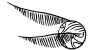
\includegraphics[scale=0.4]{boccino.png}
	\centering
\end{figure}

Il negozio di bauli era più riccamente arredato di ogni altro negozio che Harry avesse visitato; le tende avevano decori lussuosi e delicati, il pavimento e le pareti erano di legno dipinto e lucidato, e i bauli occupavano posti d’onore su piattaforme in avorio lucidato. Il commesso era vestito con abiti eleganti, appena una spanna al di sotto di quelli di Lucius Malfoy, e parlò con una cortesia squisita e melliflua sia a Harry sia alla professoressa McGonagall.

Harry aveva fatto le sue domande, e aveva gravitato verso un baule di legno dall’aspetto pesante, non lucido ma caldo e solido, scolpito con il motivo di un drago guardiano i cui occhi si muovevano per guardare chiunque si avvicinasse. Un baule incantato per essere leggero, per ridursi a comando, per far spuntare piccoli tentacoli artigliati dal fondo e dimenarsi dietro al suo proprietario. Un baule con due cassetti su ognuno dei quattro lati, ciascuno che scivolava fuori per rivelare compartimenti profondi come l’intero baule. Un coperchio con quattro serrature, ognuna delle quali avrebbe rivelato uno spazio diverso all’interno. E — questa era la parte più importante — una maniglia sul fondo che faceva scivolare fuori un telaio contenente una scala che portava giù in una piccola stanza illuminata, la quale poteva contenere, Harry stimò, circa dodici librerie.

Se realizzavano bauli come quello, Harry non sapeva perché qualcuno si disturbasse a possedere una casa.

Cento e otto galeoni d’oro. Quello era il prezzo di un buon baule, appena usato. Con circa cinquanta sterline britanniche per un galeone, era abbastanza per comprare una macchina di seconda mano. Sarebbe stato più costoso di ogni altra cosa che Harry avesse comprato in tutta la sua vita messa insieme.

Novantasette galeoni. Tanto era rimasto nella borsa d’oro che Harry era stato autorizzato a prelevare da Gringotts.

La professoressa McGonagall aveva un’espressione di disappunto sul suo viso. Alla fine di una lunga giornata di acquisti, non aveva bisogno di chiedere a Harry quanto oro fosse rimasto nella borsa, dopo che il venditore aveva annunciato il suo prezzo, il che significava che la Professoressa era in grado di fare i conti mentalmente, senza carta e penna. Ancora una volta, Harry dovette ricordare a sé stesso che \textit{analfabeta scientifico} non era affatto la stessa cosa di \textit{stupido}.

«Mi dispiace, giovanotto», disse la professoressa McGonagall. «È tutta colpa mia. Le proporrei di riportarla da Gringotts, ma la banca sarà chiusa per tutti i servizi tranne quelli di emergenza, ora.»

Harry la osservò, chiedendosi…

«Bene», sospirò la professoressa McGonagall, mentre girò facendo perno su di un tallone, «allora possiamo andare, presumo.»

… \textit{non aveva} perso del tutto il controllo quando un bambino aveva osato sfidarla. Non ne era stata contenta, ma aveva \textit{pensato} invece di lasciare che la sua rabbia esplodesse. Poteva essere semplicemente perché c’era un Signore Oscuro immortale da combattere — perché aveva bisogno della buona volontà di Harry. Ma la maggior parte degli adulti non sarebbe stata in grado di pensare neppure quello; non avrebbero affatto considerato le \textit{conseguenze future}, se qualcuno di uno status inferiore si fosse rifiutato di obbedire loro…

«Professoressa?» disse Harry.

La strega si girò per guardarlo.

Harry fece un respiro profondo. Aveva bisogno di essere un po’ arrabbiato per fare ciò che voleva provare, era impossibile che trovasse il coraggio di farlo in caso contrario. \textit{Non mi ha ascoltato}, pensò, \textit{io avrei preso più oro, ma lei non mi ha ascoltato…} Concentrando tutto il suo mondo sulla McGonagall e sulla necessità di piegare quella conversazione alla propria volontà, parlò.

«Professoressa, lei pensava che cento galeoni sarebbero stati più che sufficienti per un baule. Ecco perché non si è presa il disturbo di avvertirmi prima che scendessero a novantasette. Il che è proprio il genere di cose che le ricerche dimostrano — questo è quello che succede quando le persone pensano di essersi lasciate un \textit{piccolo} margine di errore. Non sono abbastanza pessimiste. Se fosse stato per me, avrei preso \textit{duecento} galeoni giusto per essere sicuri. C’era abbondanza di soldi in quel deposito, e avrei potuto rimetterci quelli in eccesso successivamente. Ma ho pensato che non mi avrebbe permesso di farlo. Ho pensato che si sarebbe arrabbiata con me se solo l’avessi chiesto. Sbagliavo?»

«Suppongo di dover confessare che ha ragione», disse la professoressa McGonagall. «Ma, giovanotto –»

«Questo genere di cose è la ragione per cui ho difficoltà a fidarmi degli adulti.» In qualche modo Harry mantenne la voce salda. «Perché si arrabbiano se solo \textit{provi} a ragionare con loro. Per loro si tratta di un atteggiamento di ribellione e di insolenza, una sfida al loro status tribale superiore. Se tenti di parlare con loro si \textit{arrabbiano}. Quindi, se avessi qualcosa di \textit{veramente importante} da fare, non sarei in grado di fidarmi di lei. Anche se ascoltasse con profondo interesse ciò che le dicessi — perché anche questo fa parte del ruolo di qualcuno che interpreta la \textit{parte} dell’adulto interessato — non cambierebbe mai le sue azioni, non si comporterebbe mai realmente in modo differente, a causa di qualcosa che le avessi detto io.»

Il commesso li stava guardando entrambi con palese affascinazione.

«Posso capire il suo punto di vista», disse infine la professoressa McGonagall. «Se a volte sembro troppo severa, la prego di non scordare che ho servito come Preside di Casa Grifondoro per un tempo che mi sembra pari a diverse migliaia di anni.»

Harry annuì e continuò. «Quindi — supponga che io abbia il modo di prelevare altri galeoni dal mio deposito senza essere costretti a tornare alla Gringotts, ma che questo implichi una mia violazione del ruolo di bambino obbediente. Poteri fidarmi di lei per questa faccenda, anche se questo l’obbligasse ad abbandonare il suo ruolo di professoressa McGonagall per trarne vantaggio?»

«\textit{Cosa?}» esclamò la professoressa McGonagall.

«Per metterla in un’altra maniera, se potessi far sì che la giornata di oggi fosse andata in maniera differente, in modo che \textit{non avessimo} portato con noi denaro insufficiente, sarebbe questo accettabile, anche se implicherebbe che un bambino sia stato insolente verso un adulto, a posteriori?»

«Suppongo… di sì…» disse la strega, sembrando alquanto perplessa.

Harry prese la borsa mokeskin, e disse, «Undici galeoni provenienti dal mio deposito di famiglia.»

E ci fu dell’oro nella mano di Harry.

Per un momento la professoressa McGonagall rimase a bocca aperta, poi la sua mascella di chiuse di scatto e i suoi occhi formarono una fessura e la strega disse con una rabbia controllata, «\textit{Dove} ha preso quel –»

«Dal mio deposito di famiglia, come ho detto.»

«\textit{Come?}»

«Magia.»

«Questa non è una risposta!» scattò la professoressa McGonagall, e poi si fermò, battendo gli occhi.

«No, non lo è, vero? \textit{Dovrei} affermare di aver scoperto sperimentalmente il vero segreto del funzionamento della borsa e che può effettivamente recuperare gli oggetti da qualunque luogo, non solo dal proprio interno, se si formula la richiesta correttamente. Ma in realtà li ho presi prima, quando sono caduto in quel mucchio d’oro e ho spinto alcuni galeoni in tasca. Chiunque capisca il pessimismo sa che il denaro è qualcosa di cui potresti aver bisogno rapidamente e senza molto preavviso. Dunque ora è arrabbiata con me per aver sfidato la sua autorità? O felice perché abbiamo portato a termine la nostra importante missione?»

Gli occhi del commesso erano spalancati per lo stupore.

E l’alta strega restò ferma, in silenzio.

«A Hogwarts la disciplina \textit{deve} essere rispettata», disse dopo quasi un intero minuto. «Per il bene di \textit{tutti} gli studenti. E questo \textit{deve} includere cortesia e obbedienza da parte sua verso \textit{tutti} i professori.»

«Comprendo, professoressa McGonagall.»

«Bene, ora compriamo quel baule e andiamo a casa.»

Harry si sentì come se stesse per vomitare, o per esultare, o per svenire, o \textit{qualcosa}. Era la prima volta che il suo ragionamento attento aveva mai funzionato con \textit{chiunque}. Forse perché era la prima volta che aveva qualcosa di davvero importante di cui un adulto aveva bisogno, eppure –

Minerva McGonagall, +1 punto.

Harry fece un inchino, e mise la borsa d’oro e gli undici galeoni extra nelle mani di McGonagall. «La ringrazio di cuore, professoressa. Può completare l’acquisto per me? Devo far visita al bagno.»

Il commesso, nuovamente mellifluo, indicò in direzione di una porta inserita nel muro, con una maniglia dorata. Appena Harry iniziò ad allontanarsi, sentì il commesso chiedere nella sua voce melliflua, «Posso domandare chi sia quella persona, Madam McGonagall? Presumo sia un Serpeverde — del terzo anno, forse? — e di famiglia illustre, ma non ho riconosciuto –»

Il rumore della porta del bagno che si chiudeva interruppe le sue parole, e dopo che Harry ebbe individuato il nottolino di chiusura e l’ebbe azionato, afferrò l’asciugamano magico auto-pulente e, con le mani tremanti, si tolse il sudore dalla fronte. L’intero corpo di Harry era ricoperto di sudore, che aveva impregnato i suoi abiti babbani, sebbene, quanto meno, non si vedesse attraverso le vesti da mago.

\begin{figure}[h]
	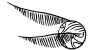
\includegraphics[scale=0.4]{boccino.png}
	\centering
\end{figure}

Il sole stava tramontando ed era effettivamente molto tardi, quando si trovarono nuovamente nel cortile del Paiolo Magico, la silenziosa e fronzuta interfaccia tra la Diagon Alley della Gran Bretagna magica e l’intero mondo babbano. (Si trattava di un’economia disaccoppiata in maniera \textit{terribile}…) Una volta arrivato dall’altra parte, Harry raggiunse una cabina telefonica e chiamò suo padre. Non aveva bisogno di preoccuparsi che il suo bagaglio venisse rubato, apparentemente. Il suo baule godeva della condizione di oggetto magico maggiore, qualcosa che la maggior parte dei Babbani non notava neppure; quello era parte di ciò che potevi ottenere nel mondo magico, se eri disposto a pagare il prezzo di un’auto di seconda mano.

«Quindi le nostre strade si dividono qui, per ora», disse la professoressa McGonagall. Scosse la testa per la meraviglia. «Questo è stato il giorno più strano della mia vita da… diversi anni. Sin dal giorno in cui venni a sapere che un bambino aveva sconfitto Tu-Sai-Chi. Oggi mi chiedo, guardandomi indietro, se quello sia stato l’ultimo giorno ragionevole del mondo.»

Oh, come se \textit{lei} avesse qualcosa di cui lamentarsi. \textit{Pensi che la tua giornata sia stata surreale? Prova la mia.}

«Sono stato molto colpito da lei, oggi», le disse Harry. «Avrei dovuto ricordarmi di farle i complimenti ad alta voce, nella mia mente le stavo assegnando dei punti.»

«Grazie, signor Potter», disse la professoressa McGonagall. «Se fosse stato già assegnato a una Casa, le avrei sottratto talmente tanti punti che i suoi nipoti starebbero ancora perdendo la Coppa delle Case».

«Grazie a \textit{lei}, Professoressa». Era probabilmente ancora troppo presto per chiamarla Minnie.

Questa donna sarebbe potuta essere l’adulto più sano di mente che Harry avesse mai incontrato, malgrado la mancanza di un’educazione scientifica. Harry stava anche considerando di offrirle la posizione numero due in qualunque gruppo avesse formato per combattere il Signore Oscuro, sebbene non fosse abbastanza folle da dirlo ad alta voce. \textit{E quale sarebbe un nome appropriato per questo gruppo…? I Mangiamangiamorte?}

«La vedrò presto, quando inizierà la scuola», disse la professoressa McGonagall. «E, signor Potter, riguardo alla sua bacchetta –»

«So cosa sta per chiedermi», disse Harry. Tirò fuori la sua preziosa bacchetta e, con una profonda fitta di pena interiore, la fece ruotare nella mano, in modo da offrirle l’impugnatura. «La prenda. Non avevo intenzione di farci nulla, proprio niente, ma non voglio che abbia incubi in cui faccio saltare in aria la mia casa.»

La professoressa McGonagall scosse la testa rapidamente. «Oh no, signor Potter! Non si tratta di questo. Volevo solo avvisarla di non usare la sua bacchetta a casa, in quanto il Ministero è in grado di rilevare la pratica magica da parte di minori, ed è proibita in assenza di supervisori.»

«Ah», disse Harry. «Mi sembra una regola ragionevole. Sono contento di vedere che il mondo della magia prende sul serio questo genere di cose.»

La professoressa McGonagall lo fissò attentamente. «Sta dicendo sul serio.»

«Sì», rispose Harry. «Lo capisco. La magia è pericolosa e le regole esistono per buone ragioni. Anche altre faccende sono pericolose. Capisco anche quello. Si ricordi che non sono stupido.»

«È improbabile che me lo dimentichi. Grazie, Harry, questo mi fa sentire meglio a proposito delle altre cose che ti ho confidato. Arrivederci, per ora.»

Harry si girò per andarsene, nel Paiolo Magico e poi fuori verso il mondo dei Babbani.

Mentre la sua mano toccava la maniglia della porta sul retro, sentì un ultimo sussurro da dietro di sé.

«Hermione Granger.»

«Cosa?» disse Harry con la mano ancora sulla maniglia.

«Cerca una ragazza del primo anno chiamata Hermione Granger sul treno per Hogwarts.»

«Chi è?»

Non ci fu risposta, e quando Harry si girò, la professoressa McGonagall se n’era andata.

\begin{figure}[h]
	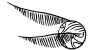
\includegraphics[scale=0.4]{boccino.png}
	\centering
\end{figure}

\subsubsection{Conseguenze}

Il preside Albus Silente si chinò in avanti sulla propria scrivania. I suoi occhi sfavillanti indagarono Minerva. «Dunque, mia cara, come hai trovato Harry?»

Minerva aprì la bocca. Poi chiuse la bocca. Poi aprì la bocca ancora una volta. Nessuna parola ne uscì.

«Capisco», disse Albus seriamente. «Grazie per la tua relazione, Minerva. Puoi andare.»

% !TeX root = Harry.tex

\chapter{Reciprocità}
\label{capitolo:7}

\emph{«Tuo padre è quasi tanto fantastico quanto il mio.»}

~\\
~\\

Le labbra di Petunia Evans-Verres stavano tremando, e i suoi occhi riempiendosi di lacrime, mentre Harry l’abbracciava alla vita al Binario Nove della stazione di King’s Cross. «Sei sicuro di non volere che venga con te, Harry?»

Harry lanciò un’occhiata a suo padre Michael Verres-Evans, che sembrava lo stereotipo del severo-ma-fiero, e poi di nuovo a sua madre, che aveva davvero un aspetto piuttosto… non composto. «Mamma, so che il mondo dei maghi non ti piace molto. Non devi venire con me. Dico sul serio.»

Petunia fece una smorfia. «Harry, non dovresti preoccuparti per me, io sono tua madre e se hai bisogno di qualcuno con te –»

«Mamma, starò da solo a Hogwarts per \textit{mesi} e \textit{mesi}. Se non riesco a sopportare una piattaforma del treno da solo, meglio scoprirlo il più presto possibile in modo che possiamo annullare tutto.» Abbassò la voce a un sussurro. «E poi, mamma, tutti mi amano laggiù. Se avessi dei problemi, tutto quello che dovrò fare è togliermi la fascia», Harry toccò la fascetta ginnica che copriva la sua cicatrice, «e avrò \textit{molto} più aiuto di quanto io possa gestire.»

«Oh, Harry», sussurrò Petunia. Si inginocchiò e lo abbracciò forte, viso contro viso, le guance appoggiate l’una contro l’altra. Harry poté percepire il suo respiro irregolare, e poi sentì un singhiozzo soffocato sfuggirle. «Oh, Harry, ti voglio bene davvero, ricordalo sempre.»

\textit{È come se avesse paura di non vedermi mai più}, il pensiero nacque improvviso nella mente di Harry. Sapeva che il pensiero era vero, ma non sapeva perché la mamma avesse tanta paura.

Così tirò a indovinare. «Mamma, lo sai che non ho intenzione di trasformarmi in tua sorella solo perché sto imparando la magia, giusto? Farò qualsiasi magia mi chiederai — se posso, voglio dire — o se vorrai che io non usi nessuna magia a casa, farò anche questo, prometto che non lascerò mai che la magia si intrometta tra noi –»

Un forte abbraccio interruppe le sue parole. «Hai un buon cuore», sua madre gli sussurrò nell’orecchio. «Un cuore davvero buono, figlio mio.»

Harry rimase allora senza parole.

Sua madre lo lasciò e si alzò. Prese un fazzoletto dalla borsetta e con mano tremante tamponò il trucco che le colava intorno agli occhi.

Non c’erano dubbi sulla possibilità che suo padre lo accompagnasse dal lato magico della stazione di King’s Cross. Papà aveva problemi anche solo a guardare esplicitamente il baule di Harry. La magia scorreva nel sangue delle famiglie, e in Michael Verres-Evans non riusciva neppure a gocciolare.

Così invece il padre si schiarì appena la gola. «Buona fortuna per la scuola, Harry», disse. «Pensi che ti abbia comprato abbastanza libri?»

Harry aveva spiegato a suo padre di come avesse pensato che questa potesse essere la sua grande occasione per fare qualcosa di veramente rivoluzionario e importante, e il professor Verres-Evans aveva annuito e messo da parte la sua fitta agenda per due intere giornate allo scopo di dedicarsi al Più Grande Giro delle Librerie di Seconda Mano di Sempre, che aveva coperto quattro città e prodotto trenta casse di libri scientifici che ora giacevano nel livello sotterraneo del baule di Harry. La maggior parte dei libri erano andati via per una sterlina o due, ma alcuni di loro decisamente \textit{no}, come il più recente \textit{Manuale di Chimica e Fisica} o l’edizione completa del 1972 della \textit{Encyclopædia Britannica}. Suo padre aveva cercato di impedire a Harry di vedere gli schermi dei registratori di cassa, ma Harry aveva capito che doveva aver speso \textit{almeno} un migliaio di sterline. Harry aveva detto a suo padre che lo avrebbe ripagato non appena avesse capito come convertire l’oro dei maghi in denaro babbano, e suo padre gli aveva detto di andare a buttarsi in un lago.

E poi suo padre gli aveva chiesto: \textit{Pensi che ti abbia comprato abbastanza libri?} Era sufficientemente chiaro quale risposta Papà volesse sentire.

La voce di Harry era rauca, per qualche ragione. «Non è possibile avere abbastanza libri», disse recitando il motto della famiglia Verres, e suo padre si inginocchiò e gli diede un rapido e saldo abbraccio. «Ma \textit{certamente} ci hai provato», disse Harry, e si sentì soffocare di nuovo. «È stato davvero, \textit{davvero}, davvero un buon tentativo.»

Suo padre si raddrizzò. «Allora…», disse. «Lo vedi \textit{tu} il Binario Nove e Tre Quarti?»

La stazione di King’s Cross era enorme e trafficata, con pareti e pavimenti lastricati di ordinarie piastrelle macchiate di sporco. Era piena di persone ordinarie che si affrettavano nei loro affari ordinari, tenendo conversazioni ordinarie che causavano grandi quantità di rumore ordinario. La stazione di King’s Cross aveva un Binario Nove (su cui erano) e un Binario Dieci (proprio a fianco), ma non c’era niente tra il Binario Nove e il Binario Dieci, a parte un muro divisorio sottile e poco promettente. Un grande lucernario sulle loro teste lasciava entrare molta luce che illuminava la totale mancanza di qualunque Binario Nove e Tre Quarti.

Harry si guardò intorno fino a quando i suoi occhi non si inumidirono, pensando, \textit{forza, vista da mago, forza, vista da mago}, ma non apparve assolutamente nulla. Pensò di prendere la bacchetta e agitarla, ma la professoressa McGonagall lo aveva avvertito di non usarla. Inoltre, se ci fosse stata un’altra pioggia di scintille multicolori, l’avrebbero potuto arrestare per accensione di fuochi d’artificio all’interno di una stazione ferroviaria. E questo assumendo che la sua bacchetta non avesse deciso di fare qualcos’altro, come far saltare in aria l’intera King’s Cross. Harry aveva dato appena un’occhiata i suoi libri di scuola (anche se quell’occhiata era stata piuttosto bizzarra) nel rapido sforzo di determinare che tipo di libri di scienza avrebbe dovuto acquistare nelle 48 ore successive.

Bene, aveva — Harry guardò l’orologio — un’ora intera per capirlo, visto che doveva essere sul treno per le undici. Forse questo era l’equivalente di un test di qi e i bambini stupidi non potevano diventare maghi. (E la quantità di tempo in più che ti lasciavi avrebbe determinato la tua Coscienziosità, che era il secondo fattore più importante per il successo accademico.)

«Lo scoprirò», disse Harry ai suoi genitori in attesa. «Probabilmente è una specie di prova.»

Suo padre si accigliò. «Uhm… forse dovresti cercare per terra una traccia formata da impronte diverse, che porta da qualche parte che non sembra avere senso –»

«\textit{Papà!}» disse Harry. «Smettila! Non ho neppure \textit{provato} a capirlo da solo!» Era un ottimo suggerimento, persino, il che era peggio.

«Mi dispiace», si scusò il padre.

«Ah…», disse la madre di Harry. «Non credo che farebbero questo a uno studente, e tu? Sei sicuro che la professoressa McGonagall non ti abbia detto niente?»

«Forse è stata distratta», disse Harry senza pensare.

«\textit{Harry!}» sibilarono il padre e la madre all’unisono. «\textit{Che cosa hai fatto?}»

«Io, uhm –» Harry deglutì. «Guardate, non abbiamo tempo ora per questo –»

«\textit{Harry!}»

«Dico sul serio! Non abbiamo tempo ora per questo! Perché è una storia molto lunga e devo capire come arrivare a scuola!»

Sua madre aveva una mano sul viso. «Quanto è grave?»

«Io, ah», \textit{non posso parlarne per ragioni di sicurezza nazionale}, «circa la metà dell’Incidente con il progetto di scienze?»

«\textit{Harry!}»

«Io, ehm, oh guardate ci sono alcune persone con un gufo andrò a chiedergli come entrare!» e Harry fuggì via dai suoi genitori verso la famiglia dai capelli rosso fuoco, il suo baule che strisciò automaticamente dietro di lui.

La donna grassoccia lo guardò mentre si avvicinava. «Ciao, caro. Prima volta a Hogwarts? Anche Ron è nuovo, –» e poi lo scrutò attentamente. «\textit{Harry Potter?}»

Quattro ragazzi e una ragazza dai capelli rossi e un gufo si voltarono all’unisono e rimasero pietrificati sul posto.

«Oh, \textit{andiamo!}» protestò Harry. Aveva progettato di farsi passare per Harry Verres, almeno fino all’arrivo a Hogwarts. «Ho comprato una fascia e tutto il resto! Come fa a sapere chi sono?»

«Sì», disse il padre di Harry, giungendogli alle spalle con lunghi passi agili, «come \textit{fa} a sapere chi è?» La sua voce mostrava un certo timore.

«La tua foto era sui giornali», disse uno dei due gemelli di aspetto identico.

«\textsc{harry!}»

«\textit{Papà!} Non è come pensi! È perché ho sconfitto il Signore Oscuro Tu-Sai-Chi quando avevo un anno!»

«\textsc{cosa?}»

«La mamma può spiegare.»

«\textsc{cosa?}»

«Ah… Michael caro, ci sono alcune cose, ho pensato, con le quali sarebbe stato meglio non seccarti fino a ora –»

«Scusatemi», disse Harry alla famiglia dai capelli rossi che lo stava fissando al completo, «ma sarebbe davvero estremamente utile se poteste dirmi come arrivare al Binario Nove e Tre Quarti \textit{in questo preciso momento.}»

«Ah…» disse la donna. Alzò una mano e indicò il muro tra i binari. «Basta camminare dritto verso la barriera tra i Binari Nove e Dieci. Non fermarti e non aver paura di sbatterci contro, questo è molto importante. Meglio prendere un po’ di rincorsa, se sei nervoso.»

«E qualunque cosa tu faccia, non pensare a un elefante.»

«\textit{George!} Ignoralo, Harry caro, non c’è motivo per non pensare a un elefante.»

«Sono Fred, mamma, non George –»

«Grazie!» disse Harry e prese a correre verso la barriera –

Un attimo, non avrebbe funzionato \textit{se non ci avesse creduto?}

Era in momenti come quello che Harry odiava la sua mente, per il fatto che funzionasse tanto velocemente da rendersi conto che si trattava di un caso di «dubbio risonante», ovvero, se avesse pensato sin dall’inizio che sarebbe passato attraverso la barriera ce l’avrebbe fatta, solo che ora si chiedeva se credeva a sufficienza che sarebbe passato attraverso la barriera, il che significava che in realtà era preoccupato di schiantarsi contro di essa –

«\textit{Harry! Torna qui, devi darmi alcune spiegazioni!» Quello era suo padre.}

Harry chiuse gli occhi e ignorò tutto ciò che sapeva sulla credibilità giustificata e cercò solo di credere davvero tanto che sarebbe passato attraverso la barriera e –

– i suoni intorno a lui cambiarono.

Harry aprì gli occhi e incespicò fino a fermarsi, sentendosi vagamente insozzato dall’aver fatto uno sforzo deliberato di credere a qualcosa.

Si trovava su di una luminosa piattaforma all’aperto, vicino a un unico enorme treno, quattordici lunghe carrozze guidate da un’imponente macchina a vapore di metallo scarlatto con un’alta ciminiera che minacciava morte alla qualità dell’aria. La piattaforma era già leggermente affollata (anche se Harry era in anticipo di un’intera ora); dozzine di bambini e i loro genitori sciamavano attorno a panche, tavoli, e vari venditori ambulanti e bancarelle.

Era scontato dire che non c’era nessun posto del genere nella stazione di King’s Cross e nessuno spazio per nasconderlo.

\textit{Va bene, allora o (a) sono stato appena teletrasportato da tutt’altra parte, o (b) possono piegare lo spazio come nessun altro oppure (c) stanno semplicemente ignorando tutte le regole.}

Ci fu un rumore strisciante dietro di lui, e Harry si voltò a osservare il suo baule che l’aveva effettivamente seguito sui propri piccoli tentacoli artigliati. Apparentemente, per quanto riguardava la magia, anche il suo bagaglio era riuscito a credere con sufficiente intensità da passare attraverso la barriera. In realtà quel pensiero fu un po’ inquietante, quando Harry lo formulò.

Un attimo dopo, il ragazzo dai capelli rossi più giovane attraversò di corsa l’arco di ferro (arco di ferro?), tirandosi dietro il baule col guinzaglio, e per poco non si schiantò contro Harry. Harry, sentendosi stupido per essere rimasto in mezzo, iniziò ad allontanarsi rapidamente dalla zona di arrivo, e il ragazzo dai capelli rossi lo seguì, strattonando con forza il guinzaglio del baule per tenere il passo. Un attimo dopo, un gufo bianco svolazzò attraverso l’arco e andò a posarsi sulla spalla del ragazzo.

«Santo cielo», disse il ragazzo dai capelli rossi, «sei \textit{davvero} Harry Potter?»

\textit{Non di nuovo}. «Non ho un modo logico di saperlo con certezza. I miei genitori mi hanno cresciuto facendomi \textit{credere} che il mio nome sia Harry James Potter-Evans-Verres, e molte persone qui mi hanno detto che \textit{assomiglio} ai miei genitori, voglio dire agli altri miei genitori, ma», Harry aggrottò la fronte, quando capì le conseguenze, «per quanto ne so \textit{io}, potrebbero facilmente esistere incantesimi che mutano le sembianze di un bambino in un aspetto specifico –»

«Eh, che hai detto, fratello?»

\textit{Non sei destinato a Corvonero, deduco}. «Sì, sono Harry Potter.»

«Sono Ron Weasley», disse l’alto ragazzo magro, lentigginoso e dal naso lungo, e gli porse una mano, che Harry educatamente strinse mentre camminavano. Il gufo rivolse a Harry un grido stranamente misurato e cortese (più che altro un suono come eehhhhh, che sorprese Harry).

A questo punto Harry si rese conto della possibilità di una catastrofe imminente. «Solo un secondo», disse a Ron, e aprì uno dei cassetti del baule, quello che se ricordava correttamente era per l’abbigliamento invernale — lo era — e poi trovò la sciarpa più leggera che avesse, sotto il cappotto invernale. Harry si tolse la fascia, e altrettanto velocemente srotolò la sciarpa e la legò intorno al viso. Era un po’ calda, soprattutto d’estate, ma Harry poteva sopportarlo.

Poi chiuse quel cassetto e ne aprì un altro e tirò fuori le vesti nere da mago, che infilò sopra la testa, ora che era fuori dal territorio babbano.

«Fatto», disse Harry. Il suono uscì un po’ ovattato dalla sciarpa sul viso. Si rivolse a Ron. «Cosa sembro? Stupido, lo so, ma sono riconoscibile come Harry Potter?»

«Ehm», disse Ron. Chiuse la bocca, che era rimasta aperta. «Non proprio, Harry».

«Molto bene», disse Harry. «Tuttavia, per non vanificare il tutto, d’ora in poi ti rivolgerai a me chiamandomi», Verres poteva non funzionare più, «signor Spoo.»

«Okay, Harry», disse Ron incerto.

\textit{La Forza non scorre potente in lui}. «Devi… chiamarmi… signor… Spoo.»

«Va bene, signor Spoo –» Ron si fermò. «Non posso farlo, mi fa sentire stupido.»

\textit{Non è solo una sensazione}. «Va bene. Scegli \textit{tu} un nome.»

«Signor Cannon», disse Ron immediatamente. «Come i Chudley Cannons.»

«Ah…» Harry sapeva che si sarebbe terribilmente pentito di averlo chiesto. «Chi o cosa sono i Chudley Cannons?»

«\textit{Chi sono i Chudley Cannons?} Solo la più grande squadra di tutta la storia del Quidditch! Certo, sono finiti ultimi in classifica lo scorso anno, ma –»

«Cos’è il Quidditch?»

Anche quella domanda fu un errore.

«Allora fammi capire bene», disse Harry mentre sembrava che la spiegazione di Ron (con il relativo gesticolare) si stesse esaurendo. «Catturare il Boccino vale \textit{centocinquanta punti?}»

«Sì –»

«Quante segnature da dieci punti realizza di solito una squadra \textit{senza} contare il Boccino?»

«Forse quindici o venti nelle partite professionistiche –»

«Questo è completamente sbagliato. Vìola ogni possibile regola di progettazione dei giochi. Ascolta, il resto di questo gioco sembra poter avere un senso, una specie, per uno sport voglio dire, ma fondamentalmente stai dicendo che la cattura del Boccino ribalta quasi tutte le differenze di punti normali. I due Cercatori sono lassù che volano in giro alla ricerca del Boccino e di solito non interagiscono con nessun altro, avvistare per primo il Boccino è per lo più fortuna –»

«Non è fortuna!» protestò Ron. «Devi muovere gli occhi seguendo lo schema giusto –»

«Non c’è \textit{interazione}, non c’è confronto con l’altro giocatore e quanto è divertente guardare qualcuno incredibilmente bravo a muovere gli occhi? E poi qualunque Cercatore abbia un colpo di fortuna, piomba giù e afferra il Boccino e rende irrilevanti tutti gli sforzi degli altri. È come se qualcuno avesse preso un gioco vero e proprio e ci avesse innestato sopra questo inutile ruolo in più in modo da poter essere il Giocatore Più Importante, senza bisogno di farsi davvero coinvolgere o imparare il resto del gioco. Chi è stato il primo Cercatore, il figlio idiota del re che voleva giocare a Quidditch, ma non riusciva a capire le regole?» In realtà, ora che Harry ci pensava, sembrava un’ipotesi sorprendentemente buona. Mettetelo su un manico di scopa e ditegli di prendere la cosa scintillante…

Il viso di Ron era contratto in una smorfia. «Se non ti piace il Quidditch, non c’è bisogno di prenderlo in giro!»

«Se non puoi criticare, non puoi ottimizzare. Sto suggerendo come \textit{migliorare il gioco}. Ed è molto semplice. Sbarazzatevi del Boccino.»

«Non cambieranno il gioco solo perché lo dici \textit{tu!}»

«Io \textit{sono} il Ragazzo-Che-È-Sopravvissuto, sai. La gente mi ascolterà. E forse se riesco a convincerli a cambiare il gioco a Hogwarts, l’innovazione si diffonderà.»

Uno sguardo di orrore assoluto si stava diffondendo sul volto di Ron. «Ma, ma se ti liberi del Boccino, come sapremo quando il gioco finisce?»

«\textit{Comprate… un… orologio}. Sarebbe molto più giusto che far finire la partita a volte dopo dieci minuti e a volte continuare per ore, e il programma sarebbe molto più prevedibile anche per gli spettatori.» Harry sospirò. «Oh, smettila di rivolgermi quello sguardo di orrore assoluto, probabilmente non userò \textit{davvero} il mio tempo per distruggere questa patetica scusa di sport nazionale e rifarlo più forte e più intelligente a mia immagine. Ho cose molto, molto, molto più importanti di cui preoccuparmi.» Harry sembrò pensieroso. «Ma del resto, non ci vorrebbe molto tempo per scrivere le Novantacinque Tesi della Riforma Senza Boccino e inchiodarle al portale di una chiesa –»

«Potter», biascicò la voce di un giovane ragazzo, «\textit{che cosa} hai sul viso e \textit{che cosa} è in piedi accanto a te?»

Lo sguardo di orrore di Ron fu sostituito da un odio totale. «\textit{Tu!}»

Harry girò la testa; e infatti era Draco Malfoy, che poteva essere stato costretto a indossare le ordinarie vesti scolastiche, ma che se lo stava facendo perdonare con un baule che sembrava almeno altrettanto magico e molto più elegante di quello di Harry, decorato in argento e smeraldi e recante ciò che Harry immaginò fosse l’emblema della famiglia Malfoy, un bellissimo serpente artigliato sovrapposto a bacchette d’avorio incrociate.

«Draco!» disse Harry. «Ehm, o Malfoy, se preferisci, anche se questo mi suona come riferito a Lucius. Sono contento di vedere che tu stia così bene dopo, uhm, il nostro ultimo incontro. Questo è Ron Weasley. E sto cercando di restare in incognito, quindi chiamami, ehm», Harry si guardò le vesti, «signor Black.»

«\textit{Harry!}» sibilò Ron. «Non puoi usare \textit{quel} nome!»

Harry sbatté le palpebre. «Perché no?» \textit{Suonava} piacevolmente oscuro, come una figura misteriosa e straniera –

«Direi che è un nome \textit{distinto}», disse Draco, «ma appartiene alla Nobile e Antichissima Casa Black. Ti chiamerò signor Argento.»

«\textit{Tu} stai lontano da… dal signor Oro», Ron disse freddamente, e fece un passo avanti. «Non ha bisogno di parlare con gente come te!»

Harry alzò conciliante una mano. «Mi farò chiamare signor Bronzo, grazie per l’ispirazione. E, Ron, uhm», Harry faticò a trovare il modo di dirlo, «sono contento che tu sia così… entusiasta di proteggermi, ma non mi dispiace particolarmente parlare con Draco –»

Apparentemente quella fu l’ultima goccia per Ron, che si girò verso Harry con gli occhi ora ardenti di sdegno. «\textit{Cosa?} Tu \textit{sai} chi è?»

«Sì, Ron, ricorderai che l’ho chiamato Draco senza che lui abbia avuto la necessità di presentarsi.»

Draco ridacchiò. Poi i suoi occhi si illuminarono alla vista del gufo bianco sulla spalla di Ron. «Oh, che cos’è \textit{questo?}» Draco chiese con un tono ricco di malizia. «Dov’è il famoso ratto della famiglia Weasley?»

«Sepolto nel cortile di casa», disse Ron freddamente.

«Oh, che tristezza. Pot… ah, signor Bronzo, dovrei menzionare che è ampiamente accettato il fatto che la famiglia Weasley sia detentrice della \textit{migliore storia di sempre riguardo gli animali domestici.} Vuoi raccontarla, Weasley?»

Il volto di Ron si contorse. «Non lo troveresti divertente se fosse successo alla \textit{tua} famiglia!»

«Oh», fece le fusa Draco, «ma non sarebbe mai \textit{accaduto} ai Malfoy.»

Le mani di Ron si chiusero a pugno –

«Basta così», disse Harry, mettendo nella voce tutta l’autorevolezza composta che poté. Era chiaro che a qualunque cosa si riferisse, quello fosse un ricordo doloroso per il ragazzo dai capelli rossi. «Se Ron non vuole parlarne, non è obbligato a farlo, e ti devo chiedere di non parlarne neppure tu.»

Draco si voltò verso Harry con uno sguardo sorpreso e Ron annuì. «Giusto, Harry! Voglio dire signor Bronzo! Vedi che tipo di persona è? Ora digli di andare via!»

Harry contò mentalmente fino a dieci, cosa che per lui fu un rapido 12345678910 — una strana abitudine rimastagli dall’età di cinque anni, quando sua madre gli aveva insegnato a farlo per la prima volta, e Harry aveva ragionato che il suo modo era più veloce e sarebbe dovuto essere altrettanto efficace. «Non gli dirò di andare via», disse Harry con calma. «È libero di parlare con me, se vuole.»

«Beh, non ho intenzione di frequentare qualcuno che frequenta Draco Malfoy», Ron annunciò freddamente.

Harry scrollò le spalle. «Dipende da te. \textit{Io} non ho intenzione di permettere a nessuno di dirmi chi posso o non posso frequentare.» In silenzio recitò, \textit{per favore vai via, per favore vai via…}

Il volto di Ron si paralizzò per la sorpresa, come se si fosse aspettato che quella frase avrebbe davvero funzionato. Poi si girò di scatto, strattonò il guinzaglio della sua valigia e si precipitò giù per la piattaforma.

«Se non ti piace», chiese Draco con curiosità, «perché non te ne sei semplicemente andato?»

«Uhm… sua madre mi ha aiutato a capire come arrivare a questo binario dalla stazione di King’s Cross, quindi era un po’ difficile dirgli di sparire. E non è che io \textit{odi} questo Ron», disse Harry, «è solo che, che…» Cercò le parole.

«Non vedi alcun motivo per il quale dovrebbe esistere?» offrì Draco.

«Più o meno.»

«In ogni caso, Potter… se davvero sei stato cresciuto da Babbani –» Draco fece una pausa qui, come se si aspettasse una smentita, ma Harry non disse niente «– allora potresti non sapere cosa significa essere famosi. La gente vuole prendersi \textit{tutto} il nostro tempo. \textit{Devi} imparare a dire di no.»

Harry annuì, assumendo un’espressione pensierosa sul volto. «Sembra un buon consiglio.»

«Se cerchi di essere gentile, finirai per spendere più tempo con i più invadenti. Decidi con chi \textit{tu} vuoi trascorrere il tuo tempo e fai andar via tutti gli altri. Sei appena arrivato, Potter, quindi tutti ti giudicheranno in base a chi frequenti, e non vuoi essere visto con persone come Ron Weasley.»

Harry annuì di nuovo. «Se non ti dispiace, come hai fatto a riconoscermi?»

«\textit{Signor Bronzo}», disse Draco con voce strascicata, «ti avevo \textit{già} incontrato, ricordalo. Ho visto qualcuno che andava in giro con una sciarpa avvolta intorno alla testa, in maniera assolutamente ridicola. Così ho tirato a \textit{indovinare.}»

Harry chinò il capo, accettando il complimento. «Sono \textit{terribilmente} dispiaciuto per quello che è accaduto», disse Harry. «Il nostro primo incontro, voglio dire. Non volevo metterti in imbarazzo davanti a Lucius.»

Draco agitò la mano indirizzando a Harry uno sguardo strano. «Vorrei solo che mio Padre fosse entrato mentre \textit{tu} stavi lusingando \textit{me} –» Draco rise. «Ma grazie per ciò che \textit{tu} hai detto a mio Padre. Se non fosse stato per quello, sarebbe stato più difficile dare una spiegazione.»

Harry gli rivolse un inchino più profondo. «E grazie a \textit{te} per aver ricambiato con quello che hai detto alla professoressa McGonagall.»

«Non c’è di che. Anche se una delle assistenti deve aver chiesto alla sua migliore amica di giurare di mantenere il segreto assoluto, perché mio Padre dice che ci sono \textit{strane voci} in giro, come che tu e io ci saremmo azzuffati o qualcosa del genere.»

«Ahia», disse Harry, facendo una smorfia. «Sono \textit{davvero} dispiaciuto –»

«No, ci siamo abituati, Merlino sa che ci sono già parecchie voci sulla famiglia Malfoy.»

Harry annuì. «Sono contento di sentire che non sei nei guai.»

Draco fece un sorrisetto. «Mio Padre ha, ehm, un senso dell’umorismo \textit{sofisticato}, ma \textit{comprende} cosa significhi farsi degli amici. Lo comprende \textit{molto} bene. Me l’ha fatto ripetere ogni sera prima di andare a letto per tutto il mese scorso, ‘mi farò degli amici a Hogwarts’. Quando gli ho spiegato tutto e ha compreso ciò che stavo facendo, mi ha comprato un gelato.»

Harry rimase a bocca aperta. «\textit{Sei riuscito a metterla in modo che ti comprasse un gelato?}»

Draco annuì, sembrando tanto compiaciuto quanto quell’impresa meritava. «Beh, mio padre \textit{sapeva} quello che stavo facendo, ovviamente, ma è lui che mi ha insegnato \textit{come} farlo, e se sorrido nel modo giusto \textit{mentre} lo faccio, la rende una cosa tra padre e figlio e allora \textit{deve} comprarmi un gelato o gli metterò questa specie di faccia triste, come se pensassi di averlo deluso.»

Harry osservò calcolatore Draco, percependo la presenza di un altro maestro. «Hai avuto delle \textit{lezioni} su come manipolare le persone?»

«Naturalmente», disse Draco con orgoglio. «Sono un \textit{Malfoy}. Mio Padre mi ha pagato dei precettori.»

«Uau», disse Harry. Leggere \textit{Teoria e pratica della persuasione} di Robert Cialdini probabilmente non era allo stesso livello (anche se era comunque un gran bel libro). «Tuo padre è quasi tanto fantastico quanto il mio.»

Le sopracciglia di Draco si sollevarono altezzosamente. «Oh? E che cosa fa tuo padre?»

«Mi compra libri.»

Draco valutò la risposta. «Non mi sembra molto impressionante.»

«Dovevi essere presente. Comunque, sono felice di sentire tutto questo. Dal modo in cui Lucius ti stava guardando, ho pensato che stesse per c-crocifiggerti.»

«Mio padre mi ama davvero», disse Draco con fermezza. «Non l’avrebbe mai fatto.»

«Ehm…» disse Harry. Ricordava l’elegante figura dalle vesti nere e i capelli bianchi che era entrata come una furia da Madam Malkin, brandendo quel bellissimo e micidiale bastone dal manico d’argento. Non era facile immaginarselo come un padre amorevole. «Non prenderla a male, ma come fai a \textit{saperlo?}»

«Eh?» Era chiaro che si trattava di una domanda che Draco solitamente non si poneva.

«Sto ponendo la domanda fondamentale della razionalità: perché credi in ciò in cui credi? Cosa pensi di sapere e come pensi di saperlo? Cosa ti fa pensare che Lucius non ti sacrificherebbe nello stesso modo in cui sacrificherebbe ogni altra cosa per il potere?»

Draco indirizzò a Harry un altro strano sguardo. «Cosa sai esattamente \textit{tu} di mio Padre?»

«Uhm… membro del Wizengamot, membro del Consiglio Direttivo di Hogwarts, incredibilmente ricco, conosce il Ministro Fudge, ha la fiducia del Ministro Fudge, probabilmente ha alcune foto molto imbarazzanti del Ministro Fudge, è il purista del sangue più prominente ora che il Signore Oscuro è andato, ex-Mangiamorte che è stato trovato col Marchio Oscuro, ma che se l’è cavata affermando di essere stato sotto l’Incantesimo Imperius, cosa ridicolmente inverosimile e praticamente tutti lo sapevano… malvagio con la ‘\textsc{m}’ maiuscola e assassino nato… credo sia tutto.»

Gli occhi di Draco si ridussero a due fessure. «Te l’ha detto McGonagall, giusto?»

«No, non mi ha detto \textit{niente} su Lucius dopo, se non di stare lontano da lui. Quindi durante l’Incidente al negozio di pozioni, mentre la professoressa McGonagall era occupata a urlare contro il negoziante e a cercare di riportare tutto sotto controllo, ho preso da parte uno dei clienti e ho chiesto a \textit{lui} di Lucius.»

Gli occhi di Draco furono nuovamente spalancati. «L’hai fatto \textit{davvero?}»

Harry indirizzò a Draco uno sguardo perplesso. «Se ho mentito la prima volta, non ti dirò la verità solo perché me lo chiedi la seconda.»

Ci fu una certa pausa mentre Draco stava assimilando la risposta.

«Finirai certamente a Serpeverde.»

«Finirò certamente a Corvonero, grazie tante. Voglio il potere solo perché così posso ottenere i libri.»

Draco ridacchiò. «Sì, proprio. Comunque… per rispondere alla tua domanda…» Draco fece un respiro profondo, e il suo viso si fece serio. «Mio Padre una volta ha mancato un voto del Wizengamot per me. Ero su una scopa e sono caduto e mi sono rotto molte costole. Faceva davvero male. Non mi ero mai fatto così male prima e ho pensato di stare per morire. Così mio Padre ha disertato questo voto davvero importante, perché era lì accanto al mio letto al St. Mungo’s, tenendomi le mani e promettendomi che tutto sarebbe andato bene.»

Harry distolse lo sguardo per il disagio, poi, con uno sforzo, si costrinse a guardare di nuovo Draco. «Perché mi stai raccontando \textit{questo?} Sembra piuttosto… privato…»

Draco rivolse a Harry uno sguardo serio. «Uno dei miei insegnanti una volta ha detto che le persone formano amicizie strette conoscendo cose private l’una dell’altra, e la ragione per cui la maggior parte delle persone non hanno amici intimi è perché sono troppo imbarazzate per condividere qualcosa di veramente importante di sé stesse.» Draco girò in su i palmi delle mani, in un gesto di invito. «Tocca a te.»

Sapere che l’espressione speranzosa di Draco gli era stata probabilmente inculcata da mesi di pratica non la rese meno efficace, osservò Harry. In realtà la \textit{rendeva} un po’ \textit{meno} efficace, ma purtroppo non \textit{inefficace}. Lo stesso si poteva dire dell’uso intelligente da parte di Draco della pressione di ricambiare un regalo non richiesto, una tecnica che Harry aveva letto nei suoi libri di psicologia sociale (un esperimento aveva dimostrato che un dono incondizionato di \$5 era due volte più efficace di un’offerta condizionata di \$50 per convincere la gente a compilare dei sondaggi). Draco aveva fatto il dono non richiesto di una confidenza, e ora aveva invitato Harry a offrire una confidenza in cambio… e la questione era che Harry \textit{si sentiva} pressato. Un rifiuto, Harry era certo, sarebbe stato accolto con uno sguardo di triste delusione, e forse una piccola quantità di disprezzo che avrebbe indicato che Harry aveva perso punti.

«Draco, giusto per la cronaca, riconosco esattamente quello che stai facendo in questo momento. I miei libri la chiamano \textit{reciprocità} e spiegano come dare a qualcuno un regalo diretto di due sicli è risultato essere due volte più efficace che offrirgli venti sicli al fine di convincerlo a fare quello che vuoi…» Harry si interruppe.

Draco sembrava triste e deluso. «Non è un trucco, Harry. È un gesto autentico per diventare amici.»

Harry alzò una mano. «Non ho detto che non avevo intenzione di rispondere. Ho solo bisogno di tempo per trovare qualcosa che sia privato, ma altrettanto non dannoso. Come dire… volevo farti sapere che non mi si può mettere fretta.» Una pausa di riflessione poteva fare molto per disinnescare l’efficacia di molte tecniche che si basavano sulla spinta al conformismo, una volta che si avesse imparato a riconoscerle per quello che erano.

«Va bene», disse Draco. «Aspetterò mentre pensi a qualcosa. Oh, e ti prego di togliere la sciarpa mentre lo dici.»

\textit{Semplice ma efficace.}

E Harry non poté fare a meno di notare quanto goffo, impacciato e sgraziato fosse apparso il suo tentativo di resistere alla manipolazione / salvare la faccia / mettersi in mostra rispetto a Draco. \textit{Ho bisogno di quei precettori.}

«Va bene», disse Harry dopo un po’. «Ecco il mio.» Si guardò intorno e poi srotolò la sciarpa dal volto, scoprendo tutto tranne la cicatrice. «Uhm… sembra che tu possa davvero contare su tuo padre. Voglio dire… se gli parli seriamente, lui ti starà sempre ad ascoltare e ti prenderà sul serio.»

Draco annuì.

«A volte», disse Harry, e deglutì. Questo era sorprendentemente difficile, ma del resto doveva esserlo. «A volte vorrei che mio padre fosse come il tuo.» Gli occhi di Harry si ritrassero dal viso di Draco, più o meno automaticamente, e allora Harry si costrinse a guardare di nuovo Draco.

Poi Harry fu colpito da \textit{cosa diavolo aveva appena detto}, e si affrettò ad aggiungere, «Non è che vorrei che il mio Papà fosse un impeccabile strumento di morte come Lucius, mi riferivo semplicemente al prendermi sul serio –»

«Capisco», disse Draco con un sorriso. «Ecco… ora non sembra come se fossimo un po’ più vicini a essere amici?»

Harry annuì. «Già. Così sembra, in realtà. Ehm… senza offesa, ma ho intenzione di rimettermi il travestimento, \textit{davvero} non vorrei dover avere a che fare con –»

«Capisco.»

Harry abbassò nuovamente la sciarpa sul viso.

«Mio padre prende sul serio tutti i suoi amici», disse Draco. «È per questo che ha molti amici. Dovresti incontrarlo.»

«Ci penserò», disse Harry con voce neutra. Scosse la testa per la meraviglia. «Dunque tu sei davvero il suo unico punto debole. Eh.»

Ora Draco stava rivolgendo a Harry uno sguardo \textit{realmente} strano. «Vuoi andare a prendere qualcosa da bere e trovare un posto per sederci?»

Harry si rese conto che era rimasto in piedi nello stesso luogo troppo a lungo, e si stiracchiò, cercando di sbloccare la schiena. «Certo.»

Ormai la piattaforma stava iniziando a riempirsi, ma vi era ancora una zona più tranquilla sul lato lontano dal motore a vapore rosso. Lungo la strada passarono davanti a una bancarella che ospitava un uomo calvo e barbuto che offriva giornali e fumetti e lattine verde fluorescente impilate.

Il venditore stava, in effetti, sdraiato a bersi una delle lattine verde fluorescente nel momento esatto in cui vide il raffinato ed elegante Draco Malfoy che si avvicinava con un misterioso ragazzo dall’aspetto incredibilmente stupido, con una sciarpa avvolta sul viso, e questo causò al venditore un attacco di tosse improvvisa mentre beveva e gli fece rovesciare una grande quantità di liquido verde fluorescente sulla barba.

«Scusi», disse Harry, «che cos’è questa roba, esattamente?»

«SpiriTè», disse il venditore. «Se lo bevi, è destino che accada qualcosa di sorprendente che te lo fa rovesciare addosso o su qualcun altro. Ma è incantato per svanire pochi secondi più tardi –» Infatti la macchia sulla sua barba era già scomparsa.

«Che cosa divertente», disse Draco. «Che cosa davvero, davvero divertente. Venga, signor Bronzo, andiamo a cercare un altro –»

«Aspetta», disse Harry.

«\textit{Oh, andiamo!} Questo è assolutamente, assolutamente \textit{puerile!}»

«No, mi dispiace Draco, devo indagare. Cosa succede se bevo lo SpiriTè, mentre faccio del mio meglio per mantenere la conversazione del tutto seria?»

Il venditore sorrise misteriosamente. «Chi lo sa? Un amico arriva in un costume da rana? Qualcosa di inaspettato è destinato ad accadere –»

«No. Mi dispiace. Proprio non ci credo. Questo viola la mia tanto abusata sospensione dell’incredulità su così tanti livelli che non ho nemmeno le parole per descriverlo. Non esiste, non c’è proprio \textit{nessun modo} in cui una dannata \textit{bevanda} possa manipolare la realtà per produrre \textit{situazioni comiche}, oppure mollo tutto e mi ritiro alle Bahamas –»

Draco gemette. «Dobbiamo farlo \textit{veramente?}»

«Tu non devi berlo ma io \textit{devo} indagare. \textit{Devo}. Quanto?»

«Cinque zellini la lattina», disse il venditore.

«\textit{Cinque zellini?} Può vendere bevande gassate che manipolano la realtà per \textit{cinque zellini la lattina?}» Harry si mise una mano nella borsa, disse «quattro sicli, quattro zellini», e li batté sul bancone. «Due dozzine di lattine per favore.»

«Ne prendo una anch’io», sospirò Draco, e iniziò a mettere le mani nelle tasche.

Harry scosse la testa rapidamente. «Lascia stare, ci penso io, non conta neppure come favore, voglio vedere se funziona anche per te.» Prese una lattina dalla pila ora collocata sul bancone e la lanciò a Draco, poi iniziò a nutrire la propria borsa. Il Bordo Allargante della borsa ingoiò le lattine accompagnandole con ruttini, cosa che non stava proprio aiutando a ripristinare la fede di Harry nella possibilità di scoprire, un giorno, una spiegazione ragionevole per tutto ciò.

Ventidue rutti dopo, Harry teneva in mano l’ultima lattina acquistata, Draco lo guardava con un’aria di attesa, ed entrambi tirarono l’anello contemporaneamente.

Harry srotolò la sciarpa per liberare la bocca, e piegò indietro la testa per bere lo SpiriTè.

In qualche modo \textit{sapeva} di verde brillante — extra-frizzante e più «limonoso» del limone.

A parte ciò, null’altro accadde.

Harry guardò il venditore, che li stava osservando con benevolenza.

\textit{Va bene, se questo tizio ha appena approfittato di un incidente naturale per vendermi ventiquattro lattine di niente, applaudirò il suo spirito imprenditoriale creativo e poi lo ucciderò.}

«Non sempre accade subito», disse il venditore. «Ma è garantito che accada una volta per lattina, o sarete rimborsati.»

Harry bevette un altro lungo sorso.

Ancora una volta, non accadde nulla.

\textit{Forse dovrei solo tracannare tutto il più velocemente possibile… e sperare che il mio stomaco non esploda per tutto il biossido di carbonio, o che io non faccia un rutto mentre lo bevo…}

No, poteva permettersi di avere un po’ di pazienza. Ma in tutta onestà, Harry non vedeva come questo avrebbe potuto funzionare. Non potevi andare da qualcuno e dirgli «Ora ho intenzione di sorprenderti» oppure «E ora ho intenzione di dirti la battuta finale della barzelletta, e sarà davvero divertente.» Avresti rovinato l’effetto sorpresa. Nello stato di preparazione mentale di Harry, Lucius Malfoy sarebbe potuto passare in abiti da ballerina e non gli avrebbe causato alcun rigurgito. Con che tipo di bizzarro numero comico l’universo se ne sarebbe uscito ora?

«In ogni caso, sediamoci», disse Harry. Si preparò a bere un altro po’ di liquido e si mosse verso la distante zona d’attesa, cosa che lo mise nell’angolazione giusta per gettare uno sguardo indietro e vedere la parte del chiosco che conteneva la rastrelliera dedicata a un giornale chiamato Il Cavillo, che mostrava il seguente titolo:

\textsc{ragazzo-che-è-sopravvissuto}

\textsc{mette incinto draco malfoy}

«Gah!» urlò Draco mentre il liquido verde brillante gli fu spruzzato addosso dalla direzione di Harry. Draco si voltò verso Harry con il fuoco negli occhi e strinse la propria lattina. «Figlio di un sanguemarcio! Vediamo se a \textit{te} piace essere sputato addosso!» e diede un sorso deliberato alla lattina proprio mentre i suoi occhi scorsero il titolo.

Per puro riflesso, Harry cercò di proteggere il proprio viso mentre il getto di liquido volò nella sua direzione. Purtroppo si protesse con la mano che reggeva lo SpiriTè, mandando il resto del liquido verde a schizzare sulla propria spalla.
Harry fissò la lattina che aveva in mano anche mentre continuava a soffocare e sputacchiare e il colore verde iniziò a svanire dalla veste di Draco.


Poi alzò gli occhi e fissò il titolo del giornale.

\textsc{ragazzo-che-è-sopravvissuto}

\textsc{mette incinto draco malfoy}

Le labbra di Harry si aprirono e dissero: «ma-ma-ma-ma…»

Troppe obiezioni in concorrenza tra loro, quello era il problema. Ogni volta che Harry cercava di dire «Ma siamo solo undicenni!» l’obiezione «Ma gli uomini non possono restare incinti!» esigeva la priorità ed era poi travolta da «Ma non c’è niente tra noi, davvero!»

Poi Harry guardò nuovamente giù, verso la lattina nella sua mano.

Sentiva un profondo desiderio di fuggire via urlando a squarciagola fino a crollare per carenza d’ossigeno, e l’unica cosa che glielo impedì fu che una volta aveva letto che il panico completo era il segno di un problema scientifico \textit{veramente} importante.

Harry ringhiò, gettò con forza la lattina in un vicino cestino della spazzatura, e tornò di nuovo verso la bancarella. «Una copia de \textit{Il Cavillo}, prego.» Harry pagò altri quattro zellini, recuperò un’altra lattina di SpiriTè dalla borsa, e poi si diresse verso l’area picnic con il ragazzo dai capelli biondi, il quale fissava la propria lattina con un’espressione di sincera ammirazione.

«Ritiro tutto», disse Draco, «è stato davvero notevole.»

«Ehi, Draco, sai cosa scommetto che sia ancor meglio per diventare amici dello scambiarsi i segreti? Commettere un omicidio.»

«Ho un precettore che la pensa così», ammise Draco. Portò la mano sotto le vesti e si grattò con un movimento naturale e tranquillo. «Chi hai in mente?»

Harry sbatté \textit{Il Cavillo} giù duro sul tavolo da picnic. «Il tipo che si è inventato questo titolo.»

Draco gemette. «Non un tipo. Una tipa. Una tipa di \textit{dieci anni}, riesci a crederci? È impazzita dopo che sua madre è morta e suo padre, che possiede questo giornale, è \textit{convinto} che lei sia una veggente, così quando non sa qualcosa chiede a Luna Lovegood e crede a \textit{tutto} ciò che dice.»

Senza pensarci, Harry tirò l’anello della successiva lattina di SpiriTè e si preparò a bere. «Mi stai prendendo in giro? Questo è anche peggio del giornalismo babbano, cosa che avrei pensato fosse fisicamente impossibile.»

Draco ringhiò. «Lei ha un’ossessione perversa per i Malfoy, per di più, e suo padre ci è politicamente avverso, quindi ne pubblica ogni parola. Non appena sarò abbastanza grande ho intenzione di violentarla.»

Liquido verde schizzò fuori dalle narici di Harry, bagnando la sciarpa che ancora copriva quella parte. SpiriTè e polmoni non andavano d’accordo, e Harry trascorse i successivi secondi tossendo freneticamente.

Draco lo guardò attentamente. «Qualcosa non va?»

Fu allora che Harry giunse all’improvvisa realizzazione che (a) i suoni provenienti dal resto della piattaforma del treno si erano trasformati in un rumore bianco indistinto all’incirca quando Draco aveva messo la mano sotto le vesti, e (b) quando aveva parlato del commettere un omicidio come un metodo per stringere i legami, vi era stata esattamente una persona nella conversazione che aveva pensato che stessero scherzando.

\textit{Già. Perché lui sembrava un ragazzo tanto normale. Ed era un ragazzo normale, era proprio quello che ci si aspetterebbe che fosse un bambino medio se Darth Vader fosse il suo padre affettuoso.}

«Sì, beh», Harry tossì, oh dio, come avrebbe fatto a uscire da questo vicolo cieco colloquiale, «ero solo sorpreso di quanto fossi disposto a discuterne così apertamente, non sembravi preoccupato di essere arrestato o altro.»

Draco sbuffò. «Stai scherzando? La parola di \textit{Luna Lovegood} contro la mia?»

Porca miseriaccia. «Non esiste una cosa come il rilevamento magico della verità, ne deduco?» \textit{O il test del \textsc{dna}… per ora.}

Draco si guardò intorno. I suoi occhi si strinsero. «Già, tu non ne sai niente. Senti, ti spiegherò come stanno le cose, voglio dire il modo in cui funzionano davvero, proprio come se tu fossi già a Serpeverde e mi avessi fatto la stessa domanda. Ma devi giurare di non dire nulla a riguardo.»

«Lo giuro», disse Harry.

«I tribunali usano il Veritaserum, ma è davvero uno scherzo, basta farti Obliare prima di testimoniare e poi sostenere che l’altra persona abbia ricevuto un ricordo falso con l’Incantesimo di Memoria. Naturalmente se sei una persona comune, i giudici propendono per l’Obliazione, non per un Incantesimo del Falso Ricordo. Ma la corte ha potere discrezionale, e se fossi coinvolto \textit{io} allora andrebbe a ledere l’onore di una Nobile Casa, così si andrebbe al Wizengamot, dove mio Padre ha la maggioranza. Dopo che fossi dichiarato innocente, la famiglia Lovegood dovrebbe pagare un risarcimento per aver infangato il mio onore. E sanno fin dall’inizio che è così che andrà, così tengono semplicemente la bocca chiusa.»

Un brivido freddo discese su Harry, un freddo che venne con l’istruzione di mantenere il viso e la voce normali. \textit{Nota a me stesso: rovescia il governo della Gran Bretagna magica alla prima occasione.}

Harry tossì di nuovo per schiarirsi la voce. «Draco, ti prego ti prego \textit{ti prego} di non prenderla nel modo sbagliato, la mia parola mi impegna, ma come hai detto tu potrei finire a Serpeverde e voglio chiedertelo a scopo informativo, cosa succederebbe \textit{teoricamente parlando}, se \textit{io} testimoniassi che ti ho sentito progettarlo?»

«Allora, se fossi chiunque altro eccetto un Malfoy, sarei nei guai», Draco rispose con aria di sufficienza. «Dato che \textit{sono} un Malfoy… mio Padre ha la maggioranza. E poi ti schiaccerebbe… beh, credo non facilmente, perché tu \textit{sei} il Ragazzo-Che-È-Sopravvissuto, ma mio Padre è abbastanza bravo in questo genere di cose.» Draco aggrottò le sopracciglia. «E poi, \textit{tu} hai parlato di ucciderla, perché non eri preoccupato che \textit{io} testimoniassi dopo che fosse stata trovata morta?»

\textit{Come, come ha fatto questa giornata ad andare così storta?} La bocca di Harry si stava già muovendo più velocemente di quanto potesse pensare. «In quel momento pensavo che fosse più vecchia! Non so come funziona qui, ma nella Gran Bretagna babbana i tribunali sarebbero parecchio più sconvolti se qualcuno uccidesse un bambino –»

«Capisco», disse Draco, ancora un po’ sospettoso. «Ma in ogni caso, è sempre meglio se non si arriva affatto agli Auror. Se stessimo attenti a fare solo le cose che un Incantesimo di Guarigione possa rimarginare, potremmo semplicemente Obliarla in seguito e poi fare tutto da capo la settimana successiva.» Poi il ragazzo biondo ridacchiò, un acuto suono giovanile. «Anche se, immaginati solo che dica di essere stata sbattuta da Draco Malfoy e dal Ragazzo-Che-È-Sopravvissuto, nemmeno \textit{Silente} le crederebbe.»

\textit{Ho intenzione di frantumare il tuo patetico minuscolo residuo magico del Medioevo in pezzi più piccoli dei suoi atomi costituenti.} «In realtà, possiamo sospendere la faccenda? Dopo che ho scoperto che quel titolo è venuto da una ragazza di un anno più giovane di me, ho avuto un’idea diversa per la mia vendetta.»

«Eh? Racconta», disse Draco, e iniziò a bere un altro sorso del suo SpiriTè.

Harry non sapeva se l’incantesimo funzionasse più di una volta per lattina, ma sapeva che poteva evitare di assumersene la colpa, quindi fu attento a dirlo esattamente al momento giusto:

«Stavo pensando che \textit{un giorno sposerò quella donna.}»

Draco fece un suono orrido e perse del liquido verde dagli angoli della bocca come il radiatore rotto di un’automobile. «\textit{Sei impazzito?}»

«Al contrario, sono così sano di mente che brucia come il ghiaccio.»

«Hai gusti più strani di un Lestrange», disse Draco, sembrando per metà ammirato. «E suppongo che la vuoi tutta per te, eh?»

«Già. Potrei doverti un favore per questo –»

Draco agitò la mano. «Nah, questa è gratis.»

Harry fissò la lattina nella propria mano, la freddezza che si diffondeva nel sangue. Affascinante, felice, generoso di favori con i suoi amici, Draco \textit{non era} uno psicopatico. Quella era la parte triste e terribile, conoscere la psicologia umana abbastanza bene da sapere che Draco non era un mostro. C’erano state diecimila società nel corso della storia del mondo in cui quella conversazione si sarebbe potuta svolgere. No, il mondo sarebbe stato un posto molto diverso, se solo un \textit{mutante malvagio} avesse potuto dire ciò che Draco aveva detto. Era molto semplice, molto umano, era l’opinione normale se nient’altro interferiva. Per Draco, i suoi nemici non erano persone.

E nel tempo rallentato di quel paese rallentato, là e allora come nel buio-prima-dell’alba precedente l’Età della Ragione, il figlio di un nobile sufficientemente potente dava semplicemente per scontato di essere al di sopra della legge, almeno quando si trattava di una contadina qualsiasi. C’erano posti nelle terre babbane in cui funzionava ancora nello stesso modo, paesi in cui quel tipo di nobiltà esisteva ancora e ancora pensava in quel modo, o terre ancora peggiori in cui non si trattava solo della nobiltà. Era stato così in ogni luogo e tempo che non discendessero direttamente dall’Illuminismo. Una linea di discendenza, sembrava, che non includeva del tutto la Gran Bretagna magica, malgrado tutte le contaminazioni cross-culturali di cose come le lattine ad anello.

\textit{E se Draco non cambiasse idea sul suo desiderio di vendetta, e io non buttassi via la mia speranza di una vita felice per sposare una povera ragazza folle, allora tutto quello che avrei appena guadagnato è del tempo, e neppure molto…}

Per una ragazza. Non per le altre.

\textit{Mi chiedo quanto sarebbe difficile fare una lista di tutti i principali puristi del sangue e ucciderli.}

Avevano provato a fare proprio quello durante la Rivoluzione Francese, più o meno — compilare una lista di tutti i nemici del Progresso e togliere loro ogni cosa sopra al collo — e non aveva funzionato bene da quello che Harry ricordava. Forse aveva bisogno di rispolverare alcuni di quei libri di storia che suo padre gli aveva comprato, e vedere se quello che era andato storto con la Rivoluzione francese fosse qualcosa di facile da risolvere.

Harry alzò gli occhi al cielo, e alla forma pallida della Luna, visibile quella mattina nel cielo senza nuvole.

\textit{Così il mondo è guasto e imperfetto e folle, e crudele e sanguinoso e oscuro. Questa è una notizia? L’hai sempre saputo, comunque…}

«Sembri così serio», disse Draco. «Fammi indovinare, i tuoi genitori babbani ti hanno detto che questo genere di cose è malvagio.»

Harry annuì, non fidandosi molto della propria voce.

«Beh, come dice mio Padre, ci saranno pure quattro case, ma alla fine tutti appartengono o a Serpeverde o a Tassofrasso. E, francamente, non appartieni a Tassofrasso. Se decidessi di schierarti con i Malfoy sottobanco… il nostro potere e la tua reputazione… potresti cavartela per cose che neppure \textit{io} potrei fare. Vuoi \textit{provarci} per un po’? Vedere cosa vuol dire?»

\textit{Che astuto serpentello. Undici anni e già lusinghi la tua preda per farla uscire allo scoperto…}

Harry pensò, valutò, e scelse la sua arma. «Draco, mi spiegheresti la faccenda della purezza del sangue? Mi è nuova.»

Un ampio sorriso attraversò il volto di Draco. «Dovresti davvero incontrare mio Padre e chiedere a \textit{lui}, sai, è il nostro capo.»

«Dammi un accenno.»

«Va bene», disse Draco. Fece un respiro profondo, la sua voce divenne appena più grave e assunse una cadenza. «I nostri poteri sono divenuti più deboli, di generazione in generazione, mentre la contaminazione dei sanguemarcio aumenta. Mentre Salazar e Godric e Rowena e Helga fecero sorgere Hogwarts col loro potere, creando il Medaglione e la Spada e il Diadema e la Coppa, nessun mago di questi giorni sbiaditi è assurto a rivaleggiare con loro. Ci stiamo affievolendo, tutti ci stiamo affievolendo e stiamo diventando Babbani mentre ci incrociamo con la loro progenie e permettiamo ai nostri Maghinò di vivere. Se la contaminazione non sarà tenuta sotto controllo, presto le nostre bacchette si romperanno e tutte le nostre arti cesseranno, la stirpe di Merlino finirà e il sangue di Atlantide svanirà. I nostri figli non potranno che grattare la terra per sopravvivere come semplici Babbani, e l’oscurità coprirà tutto il mondo per sempre.» Draco sorbì un altro sorso dalla sua lattina, sembrando soddisfatto; quella sembrava essere l’intera argomentazione, per quanto lo riguardava.

«Persuasivo», disse Harry, intendendolo dal punto di vista descrittivo piuttosto che normativo. Era un modello consueto: la Caduta, la necessità di custodire ciò che era rimasto della purezza contro la contaminazione, il passato che si ergeva in alto e il futuro che scivolava verso il basso. E quello schema ora aveva anche una \textit{risposta}… «Devo correggerti su di un fatto, però. Le vostre informazioni sui Babbani sono un po’ arretrate. Noi non stiamo più esattamente grattando la terra.»

La testa di Draco si girò di scatto. «\textit{Cosa?} Che intendi dire con ‘\textit{noi}’?»

«Noi. Gli scienziati. La stirpe di Francesco Bacone e il sangue dei Lumi. I Babbani non si sono limitati a starsene seduti e a lamentarsi di non avere bacchette, abbiamo i \textit{nostri} poteri ora, con o senza la magia. Se tutti i vostri poteri fallissero, allora noi tutti avremmo perso qualcosa di molto prezioso, perché la vostra magia è l’unico indizio che abbiamo su come l’universo deve funzionare \textit{davvero} — ma non sareste costretti a grattare la terra. Le vostre case sarebbero ancora fresche d’estate e calde d’inverno, ci sarebbero ancora medici e medicine. La scienza può mantenervi in vita se la magia fallisse. Sarebbe una tragedia, ma non letteralmente la fine di tutta la luce del mondo. Tutto qui.»

Draco era arretrato di alcuni metri e il suo volto era pieno di paura mista a incredulità. «\textit{Nel nome di Merlino di cosa stai parlando, Potter?}»

«Ehi, ho ascoltato la \textit{tua} storia, non vuoi ascoltare la mia?» \textit{Goffo}, Harry si rimproverò, ma Draco smise realmente di arretrare e sembrò ascoltare.

«Ad ogni modo», disse Harry, «sto dicendo che pare che non abbiate fatto molta attenzione a ciò che accade nel mondo dei Babbani.» Probabilmente perché l’intero mondo magico sembrava considerare il resto della Terra come un bassofondo, meritevole della stessa copertura mediatica che il \textit{Financial Times} dedicava alle consuete agonie del Burundi. «D’accordo. Rapido controllo. I maghi sono mai stati sulla Luna? Sai, quella cosa li?» Harry indicò quel globo enorme e distante.

«\textit{Che cosa?}» disse Draco. Era abbastanza chiaro che il pensiero non era mai venuto al ragazzo. «\textit{Andare} su — è solo una –» Il suo dito puntava al coso pallido nel cielo. «Non ci si può Materializzare da qualche parte dove non si è mai stati e come potrebbe qualcuno arrivare sulla Luna, tanto per \textit{cominciare?}»

«Aspetta», disse Harry a Draco, «vorrei mostrarti un libro che ho portato con me, credo di ricordare in che scatola è.» E Harry si alzò e si inginocchiò ed estrasse le scale per il livello sotterraneo del suo baule, poi si precipitò giù per le scale e gettò via una scatola da sopra un’altra scatola, giungendo pericolosamente vicino a trattare i propri libri senza rispetto, e strappò via il coperchio della scatola e in fretta, ma con attenzione, diede un’occhiata alla pila di libri –

(Harry aveva ereditato la capacità quasi-magica dei Verres di ricordare dov’erano tutti i suoi libri, anche dopo averli visti solo una volta, cosa che era piuttosto misteriosa considerando la mancanza di qualsiasi collegamento genetico.)

E Harry corse su per la scala e la spinse di nuovo nel baule con il tallone, e, ansimando, girò le pagine del libro fino a trovare la fotografia che voleva mostrare a Draco.
Quella con il terreno bianco, secco, pieno di crateri, e le persone con le tute, e il globo bianco e blu che incombeva su tutto.


Quella fotografia.

\textit{La} fotografia, se una sola immagine in tutto il mondo fosse sopravvissuta.

«Così», disse Harry, la voce tremante perché non riusciva a nascondere completamente l’orgoglio, «è come la Terra appare dalla Luna.»

Draco si chinò lentamente. C’era una strana espressione sul suo giovane volto. «Se questa è una fotografia \textit{vera}, perché non si muove?»

\textit{Muoversi?} Oh. «I Babbani possono realizzare immagini in movimento, ma hanno bisogno di una scatola più grande per mostrarle, non possono ancora farle stare sulle singole pagine di un libro.»

Il dito di Draco si spostò su una delle tute. «Che cosa sono quelli?» La sua voce cominciava a vacillare.

«Quelli sono esseri umani. Indossano tute che coprono tutto il corpo per fornire loro l’aria, perché non c’è aria sulla Luna.»

«È impossibile», sussurrò Draco. C’era terrore nei suoi occhi, e confusione totale. «Nessun Babbano potrebbe mai farlo. \textit{Come}…»

Harry riprese il libro, sfogliò le pagine finché non trovò ciò che cercava. «Questo è un razzo che sale. Il fuoco lo spinge sempre più in alto, fino a quando non arriva alla Luna.» Girò ancora le pagine. «Questo è un razzo a terra. Questo minuscolo granello accanto a lui è una persona.» Draco rimase a bocca aperta. «Andare sulla Luna è costato l’equivalente di… probabilmente circa mille milioni di galeoni.» A Draco mancò il respiro. «E ci sono voluti gli sforzi di… probabilmente più persone di quante vivano in tutta la Gran Bretagna magica.» \textit{E quando sono arrivati, hanno lasciato una targa che diceva, ‘Siamo venuti in pace, per tutta l’umanità’. Anche se non sei ancora pronto per sentire queste parole, Draco Malfoy…}

«Stai dicendo la verità», disse Draco lentamente. «Non falsificheresti un libro intero solo per questo — e posso sentirlo nella tua voce. Ma… ma…»

«Come, senza bacchette o magia? È una lunga storia, Draco. La scienza non funziona agitando bacchette e recitando incantamenti, funziona sapendo come l’universo opera a un livello così profondo che si sa esattamente cosa fare per fargli fare quello che si vuole. Se la magia è come lanciare \textit{Imperio} su qualcuno per fargli fare quello che vuoi, allora la scienza è come conoscerlo così bene da poterlo convincere che sia sempre stata una sua idea. È molto più difficile che muovere una bacchetta, ma funziona quando le bacchette falliscono, proprio come, quando l’\textit{Imperius} fallisce, puoi ancora tentare di persuadere la persona. E la Scienza cresce di generazione in generazione. Devi \textit{veramente} sapere quello che stai facendo per fare scienza — e quando capisci davvero qualcosa, puoi spiegarla a qualcun altro. I più grandi scienziati di un secolo fa, le personalità più brillanti di cui si parla ancora con riverenza, i loro poteri non sono \textit{nulla} per i più grandi scienziati di oggi. Non vi è alcun equivalente nella scienza delle vostre arti perdute che hanno fondato Hogwarts. Nella scienza i nostri poteri aumentano ogni anno. E stiamo cominciando a capire e svelare i segreti della vita e dell’ereditarietà. Saremo in grado di guardare lo stesso sangue di cui hai parlato, e capire che cosa fa di te un mago, e tra una o due generazioni, saremo in grado di convincere quel sangue a rendere anche tutti i tuoi figli dei potenti maghi. Capisci ora, il tuo problema non è così grave come sembra, perché in un paio di decenni la scienza sarà in grado di risolverlo per te.»

«Ma…» disse Draco. La sua voce stava tremando. «Se i Babbani hanno questo tipo di potere… allora… che cosa siamo \textit{noi?}»

«No, Draco, non è così, non capisci? La scienza attinge al potere dell’intelletto umano di guardare il mondo e comprendere come funziona. Non può venir meno senza che venga meno l’umanità stessa. La tua magia potrebbe abbandonarti, e questo lo odieresti, ma tu saresti ancora \textit{tu}. Saresti ancora vivo per rammaricartene. Ma poiché la scienza si basa sulla mia intelligenza umana, è il potere che non può essere rimosso da me senza rimuovere \textit{me}. Anche se le leggi dell’universo cambiassero attorno a me, in modo che tutta la mia conoscenza non fosse più valida, mi limiterei a scoprire le nuove leggi, come è stato fatto in passato. Non è una caratteristica \textit{babbana}, è una caratteristica \textit{umana}, semplicemente affina e allena il potere che utilizzi ogni volta che guardi qualcosa che non comprendi e ti chiedi ‘Perché?’ Sei di Serpeverde, Draco, non capisci le implicazioni?»

Draco alzò lo sguardo dal libro di Harry. Il suo volto mostrava una comprensione nascente. «I Maghi possono imparare a usare questo potere.»

Con molta cautela, ora… l’esca è pronta, adesso l’amo… «Se riesci a imparare a pensare a te stesso come a un \textit{essere umano} invece che come a un \textit{mago}, allora puoi addestrare e perfezionare i tuoi poteri da essere umano.»

E se \textit{quell}’insegnamento non era in \textit{ogni} programma di scienze, Draco non aveva bisogno di saperlo, giusto?

Lo sguardo di Draco era pensieroso. «Tu l’hai… già fatto?»

«In un certo senso», ammise Harry. «La mia formazione non è completa. Non a undici anni. Ma — mio padre mi ha pagato \textit{anche} dei precettori, sai.» Certo, erano stati studenti universitari affamati, ed era stato solo perché Harry dormiva con un ciclo di 26 ore, ma meglio mettere tutto ciò da parte, per ora…

Lentamente, Draco annuì. «Pensi di poter padroneggiare \textit{entrambe} le arti, sommare i poteri insieme, e…» Draco fissò Harry. «Farti Signore dei due mondi?»

Harry fece una risata malvagia, sembrò venirgli naturale a quel punto. «Devi capire, Draco, che l’intero mondo che conosci, tutta la Gran Bretagna magica, è solo una casella di un tabellone da gioco molto più grande. Un tabellone che comprende luoghi come la Luna, e le stelle nel cielo notturno, che sono luci proprio come il Sole solo incredibilmente lontane, e cose come le galassie che sono enormemente più grandi rispetto alla Terra e al Sole, cose così grandi che solo gli scienziati possono vederle e che non sai neppure che esistono. Ma \textit{sono} realmente un Corvonero, sai, non un Serpeverde. Io non voglio dominare l’universo. Penso solo che potrebbe essere organizzato in maniera più sensata.»

C’era stupore sul volto di Draco. «Perché stai dicendo queste cose \textit{a me?}»

«Oh… non ci sono molte persone che sappiano fare \textit{vera} scienza — comprendere qualcosa per la prima volta, anche se ti confonde incredibilmente. Un aiuto sarebbe utile.»

Draco fissò Harry a bocca aperta.

«Ma non t’ingannare, Draco, la vera scienza \textit{non} è come la magia, non puoi praticarla e andartene via incontaminato come fai quando impari a pronunciare le parole di un nuovo incantesimo. Il potere ha un suo costo, un costo così alto che la maggior parte delle persone si rifiuta di pagarlo.»

Draco annuì in risposta, come se, finalmente, avesse sentito qualcosa che poteva comprendere. «E quel costo è… ?»

«Imparare ad ammettere di avere torto.»

«Uhm», Draco disse dopo che la pausa drammatica si era prolungata per un po’. «Hai intenzione di spiegarlo?»

«Quando si prova a immaginare in che modo qualcosa funziona a un livello così profondo, le prime novantanove spiegazioni che trovi sono sbagliate. La centesima è giusta. Quindi devi imparare ad ammettere che ti sbagli, più e più e più volte. Non sembra molto, ma è così difficile che gran parte delle persone non può fare scienza. Sempre mettersi in discussione, sempre ricontrollare le cose che hai dato per scontate», come avere un Boccino a Quidditch, «e ogni volta che cambi idea, cambi te stesso. Ma sto precorrendo i tempi. Li sto precorrendo parecchio. Voglio solo che tu sappia… che ti sto offrendo di condividere alcune delle mie conoscenze. Se vuoi. C’è solo una condizione.»

«Ah-a», fece Draco. «Sai, secondo mio Padre quando qualcuno ti dice così, non è mai un buon segno, mai.»

Harry annuì. «Ora, non fraintendermi pensando che stia cercando di scavare un solco tra te e tuo padre. Non si tratta di questo. È solo che voglio avere a che fare con qualcuno della mia età, e non che questo sia tra me e Lucius. Credo che anche tuo padre sarebbe d’accordo con ciò, lui sa che devi crescere prima o poi. Ma le tue mosse nella nostra partita devono essere tue. Questa è la mia condizione — che abbia a che fare con te, Draco, non con tuo padre.»

«Devo andare», disse Draco. Si alzò in piedi. «Devo andare via e rifletterci.»

«Prenditi il tuo tempo», disse Harry.

I suoni della piattaforma del treno mutarono da rumori indistinti a mormorii mentre Draco si allontanava.

Harry espirò lentamente l’aria che aveva trattenuto senza neppure rendersene conto, e poi guardò l’orologio che aveva al polso, un semplice modello meccanico che suo padre gli aveva comprato nella speranza che avrebbe funzionato in presenza di magia. La lancetta dei secondi stava ancora ticchettando, e se la lancetta dei minuti era corretta, allora non erano ancora le undici. Probabilmente sarebbe dovuto salire sul treno presto e iniziò la ricerca di comesichiama, ma gli parve che valesse la pena prendersi prima un paio di minuti per fare alcuni esercizi di respirazione e vedere se il suo sangue si sarebbe nuovamente scaldato.

Ma quando Harry alzò lo sguardo dal suo orologio, vide avvicinarsi due figure, assolutamente ridicole coi loro volti nascosti da sciarpe invernali.

«Salve, signor Bronzo», disse una delle figure mascherate. «Possiamo convincerla ad aderire all’Ordine del Caos?»

\begin{figure}[h]
	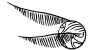
\includegraphics[scale=0.4]{boccino.png}
	\centering
\end{figure}

\subsubsection{Conseguenze}

Non molto tempo dopo, quando tutto il trambusto di quel giorno si fu finalmente placato, Draco stava chino sulla scrivania con la penna in mano. Aveva una stanza privata nei sotterranei di Serpeverde, con una scrivania propria e un proprio camino — purtroppo neppure \textit{lui} aveva diritto al collegamento al sistema via camino, ma almeno Serpeverde non aveva adottato quell’assurdità totale di far dormire \textit{tutti} nei dormitori. Non c’erano molte stanze private, bisognava essere il meglio \textit{in assoluto} all’interno della Casa dei migliori, ma questo poteva essere dato per scontato con Casa Malfoy.

\vspace{1em}
\begin{addmargin}[3em]{3em}% 1em left, 2em right
\begin{itpars}
Caro Padre, scrisse Draco.
\end{itpars}
\end{addmargin}
\vspace{1em}

E poi si fermò.

L’inchiostro gocciolò lentamente dalla sua penna, macchiando la pergamena vicino le parole.

Draco non era stupido. Era giovane, ma i suoi precettori l’avevano addestrato bene. Sapeva che probabilmente Potter si sentiva molto più vicino alla fazione di Silente di quanto non lasciasse intendere… anche se Draco pensava che Potter potesse essere tentato. Ma era chiaro che Potter stava cercando di tentare Draco proprio come Draco stava cercando di tentare lui.

Ed era anche chiaro che Potter era brillante, e ben più che un po’ matto, e stava giocando una vasta partita che Potter stesso per lo più non capiva, improvvisando a velocità massima con la sottigliezza di un Nundu infuriato. Ma Potter era riuscito a scegliere una tattica che Draco non poteva semplicemente ignorare. Aveva offerto a Draco una parte del proprio potere, puntando sul fatto che Draco non potesse usarlo senza diventare più simile a lui. Suo padre l’aveva definita una tecnica avanzata, e aveva avvertito Draco che spesso non funzionava.

Draco sapeva di non aver capito tutto quanto era accaduto… ma Potter aveva offerto a \textit{lui} la possibilità di giocare e in quel momento era sua. E se avesse spifferato tutto, sarebbe diventata di suo Padre.

Alla fine era così semplice come sembrava. Le tecniche minori richiedevano l’inconsapevolezza della vittima, o almeno la sua incertezza. L’adulazione doveva essere plausibilmente mascherata da ammirazione. («Saresti dovuto essere in Serpeverde» era un vecchio classico, altamente efficace su un certo tipo di persone che non se l’aspettavano, e se funzionava lo potevi ripetere.) Ma quando scovavi la leva decisiva di qualcuno, non importava che sapesse che tu sapevi. Potter, nella sua frenesia, aveva intuito la chiave per l’anima di Draco. E se Draco sapeva che Potter sapeva — anche se era stata un tipo di ipotesi scontata — questo non cambiava nulla.

Così ora, per la prima volta in vita sua, aveva dei veri segreti da mantenere. Stava giocando la propria partita. C’era un oscuro dolore in quello, ma sapeva che suo Padre sarebbe stato fiero, e quello rendeva tutto appropriato.

Lasciando le macchie di inchiostro al loro posto — c’era un messaggio in esse, e uno che suo padre avrebbe capito, perché avevano giocato il gioco delle sottigliezze più di una volta — Draco mise per iscritto l’unica domanda che l’aveva davvero tormentato in tutta la vicenda, la parte che sembrava che avrebbe \textit{dovuto} capire, ma non capiva, non del tutto.

\vspace{1em}
\begin{addmargin}[3em]{3em}% 1em left, 2em right
\begin{itpars}
Caro Padre,

immaginate che vi dica che ho incontrato uno studente di Hogwarts, non ancora membro della nostra cerchia di conoscenze, che vi definisce ‘un impeccabile strumento di morte’ e ha detto che sono il vostro ‘unico punto debole’. Cosa direste di lui?
\end{itpars}
\end{addmargin}
\vspace{1em}

Non ci volle molto tempo prima che la civetta di famiglia portasse la risposta.

\vspace{1em}
\begin{addmargin}[3em]{3em}% 1em left, 2em right
\begin{itpars}
Mio amato figlio,

direi che sei stato così fortunato da incontrare qualcuno che gode della fiducia intima del nostro amico e prezioso alleato, Severus Snape.
\end{itpars}
\end{addmargin}
\vspace{1em}

Draco fissò la lettera per un po’, e infine la gettò nel fuoco.

%% NEXT: Not yet formatted chapters
% !TeX root = Harry.tex

\chapter{Errore di conferma}
\label{capitolo:8}

\emph{«Permettimi di avvertirti che sfidare il mio ingegno è un genere di progetto pericoloso, e potrebbe tendere a rendere la tua vita molto più surreale.»}

~\\
~\\



Nessuno aveva chiesto il suo aiuto, quello era il problema. Se n’erano semplicemente andati in giro parlando, mangiando o guardando per aria mentre i loro genitori chiacchieravano. Per una strana ragione qualunque, nessuno era rimasto seduto a leggere un libro, e questo aveva significato che non aveva potuto semplicemente sedersi vicino a loro e tirar fuori il proprio libro. E anche quando aveva coraggiosamente preso l’iniziativa di sedersi e continuare la sua terza lettura di Storia di Hogwarts, nessuno era sembrato incline a sedersi a fianco a lei.

Oltre che aiutandole nei compiti, o in qualsiasi altra cosa di cui avessero bisogno, davvero non sapeva come conoscere le persone. Non sentiva di essere una persona timida. Pensava a sé stessa come al tipo di ragazza che si faceva carico dei problemi. Eppure, in qualche modo, se non c’era qualche richiesta del tipo «non mi ricordo come si fanno le divisioni» allora era semplicemente troppo imbarazzante andare da qualcuno e dire… cosa? Non era mai stata in grado di capire cosa. E non sembrava esserci un normale foglietto delle istruzioni, il che era ridicolo. L’intera faccenda di conoscere le persone non le era mai sembrata ragionevole. Perché doveva assumersi lei tutte le responsabilità quando erano coinvolte due persone? Perché gli adulti non erano mai d’aiuto? Desiderava solo che qualche altra ragazza venisse da lei e le dicesse «Hermione, la maestra mi ha detto di esserti amica».

Ma sia ben chiaro che Hermione Granger, seduta da sola il primo giorno di scuola in uno dei pochi scompartimenti rimasti vuoti, nell’ultima carrozza del treno, con la porta lasciata aperta nel caso in cui qualcuno per un motivo qualsiasi avesse voluto parlarle, non era triste, sola, avvilita, depressa, disperata, od ossessionata dai suoi problemi. Stava, piuttosto, rileggendo Storia di Hogwarts per la terza volta e le stava anche piacendo, con solo una lieve sfumatura di fastidio nei recessi della sua mente per l’irragionevolezza generale del mondo.

Ci fu il suono di una porta di comunicazione del treno che si apriva, e poi passi e uno strano suono strascicato che scesero lungo il corridoio della carrozza. Hermione mise da parte Storia di Hogwarts, si alzò e infilò la testa fuori — giusto nel caso in cui qualcuno avesse avuto bisogno di aiuto — e vide un giovane ragazzo in abiti da mago, forse del primo o secondo anno a giudicare dalla sua altezza, e che sembrava piuttosto sciocco con una sciarpa avvolta intorno alla testa. Un piccolo baule si trovava sul pavimento accanto a lui. Mentre lo osservava, bussò alla porta di un altro scompartimento chiuso, e disse con voce leggermente attutita dalla sciarpa, «Scusatemi, posso farvi una domanda veloce?»

Non sentì la risposta dall’interno dello scompartimento, ma dopo che il ragazzo ebbe aperto la porta, pensò davvero di averlo sentito chiedere — a meno che non avesse in qualche modo capito male — «Qualcuno qui conosce i sei quark o dove posso trovare una ragazza del primo anno di nome Hermione Granger?»

Dopo che il ragazzo ebbe chiuso la porta di quello scompartimento, Hermione gli chiese «Posso aiutarti in qualche modo?»

Il volto coperto dalla sciarpa si girò a guardarla, e la voce rispose «No, a meno che tu non possa dirmi i nomi dei sei quark o dove trovare Hermione Granger.»

«Up, down, strange, charm, truth, beauty, e perché la stai cercando?»

Era difficile dirlo da quella distanza, ma le parve di vedere il ragazzo fare un largo sorriso sotto la sciarpa. «Ah, quindi sei tu la ragazza del primo anno di nome Hermione Granger», disse quella voce giovane e attutita. «Sul treno per Hogwarts, per giunta.» Il ragazzo iniziò a camminare verso di lei e il suo scompartimento, e il suo baule scivolò dietro di lui. «Tecnicamente, tutto ciò che dovevo fare era cercarti, ma è probabile che intendesse che ti parli, o che ti inviti a entrare nel mio gruppo, o che ottenga da te un oggetto magico fondamentale, o che scopra che Hogwarts è stata costruita sopra la rovine di un antico tempio o qualcosa del genere. pg o png, questo è il problema.»

Hermione aprì la bocca per rispondere, ma poi non riuscì a formulare una qualsiasi risposta possibile… qualunque cosa fosse ciò che aveva appena sentito, anche mentre il ragazzo si avvicinò a lei, guardò all’interno dello scompartimento, annuì con soddisfazione, e sedette sul sedile di fronte al suo. Il suo baule si affrettò dietro di lui, crebbe di tre volte il suo diametro iniziale e si rannicchiò accanto a quello di lei in un modo stranamente inquietante.

«Per favore, siediti», disse il ragazzo, «e per favore, chiudi la porta dietro di te, se non ti dispiace. Non ti preoccupare, non mordo nessuno che non mi morda per primo.» Stava già srotolando la sciarpa dalla testa.

Il pensiero che questo ragazzo ritenesse che lei avesse paura di lui fece sì che la sua mano mandasse la porta scorrevole a chiudersi sbattendo contro la parete con forza eccessiva. Girò su sé stessa e vide un volto giovane con luminosi e ridenti occhi verdi, e una furiosa cicatrice rosso scuro incastonata sulla fronte che le ricordò qualcosa nei recessi della sua mente, ma in quel momento aveva cose più importanti a cui pensare. «Non ho detto di essere Hermione Granger!»

«E io non ho detto che tu hai detto di essere Hermione Granger, ho detto solo che tu sei Hermione Granger. Se stai per chiedermi come lo so, è perché so tutto. Buona sera signore e signori, il mio nome è Harry James Potter-Evans-Verres o Harry Potter in breve, so che probabilmente non significa niente per te tanto per cambiare –»

La mente di Hermione fece finalmente il collegamento. La cicatrice sulla fronte, a forma di fulmine. «Harry Potter! Sei in Storia moderna della Magia e Ascesa e declino delle Arti Oscure e Grandi eventi magici del Ventesimo secolo.» In realtà era la prima volta in tutta la sua vita che aveva incontrato qualcuno proveniente da dentro un libro, ed era una sensazione piuttosto strana.

Il ragazzo sbatté le palpebre tre volte. «Sono nei libri? Aspetta, ovviamente sono nei libri… che strano pensiero.»

«Santo cielo, non lo sapevi?» chiese Hermione. «Avrei scoperto tutto quello che potevo, se fossi stata io.»

Il ragazzo rispose piuttosto seccamente. «Signorina Granger, sono meno di 72 ore da quando sono andato a Diagon Alley e ho scoperto il motivo per cui sono famoso. Ho passato gli ultimi due giorni ad acquistare libri scientifici. Mi creda, ho intenzione di scoprire tutto ciò che posso.» Il ragazzo esitò. «Che cosa dicono i libri di me?»

La mente di Hermione Granger risentì del colpo, non si era resa conto che sarebbe stata messa alla prova su quei libri così li aveva letti solo una volta, ma era stato solo un mese fa e il materiale era ancora fresco nella sua mente. «Sei l’unico che sia sopravvissuto alla Maledizione Mortale quindi sei chiamato il Ragazzo-Che-È-Sopravvissuto. Sei nato da James Potter e Lily Potter, precedentemente Lily Evans, il 31 luglio 1980. Il 31 ottobre 1981 il Signore Oscuro, Colui-Che-Non-Deve-Essere-Nominato anche se non so perché, ha attaccato casa vostra. Sei stato trovato vivo con la cicatrice sulla fronte tra le rovine della casa dei tuoi genitori nei pressi dei resti carbonizzati del corpo di Tu-Sai-Chi. Il Capo Stregone Albus Percival Wulfric Brian Silente ti ha mandato via da qualche parte, nessuno sa dove. Ascesa e declino delle Arti Oscure sostiene che sei sopravvissuto grazie all’amore di tua madre e che la tua cicatrice contiene tutto il potere magico del Signore Oscuro e che i centauri ti temono, ma Grandi eventi magici del Ventesimo secolo non menziona nulla di simile e Storia moderna della Magia avverte che ci sono molte teorie pazzoidi su di te.»

La bocca del ragazzo era rimasta spalancata. «Ti è stato detto di aspettare Harry Potter sul treno per Hogwarts, o qualcosa del genere?»

«No», disse Hermione. «Chi ti ha parlato di me?»

«La professoressa McGonagall, e credo di capire perché. Hai una memoria eidetica, Hermione?»

Hermione scosse la testa. «Non è fotografica, ho sempre desiderato che lo fosse, ma ho dovuto leggere i miei libri di scuola per cinque volte per memorizzarli tutti.»

«Addirittura», disse il ragazzo con voce leggermente strozzata. «Spero che non ti dispiaccia se ti metto alla prova — non è che non ti creda, ma come dice il proverbio, ‘Fidati, ma verifica’. Inutile starselo a domandare quando posso sperimentalo.»

Hermione sorrise, piuttosto compiaciuta. Amava tanto gli esami. «Fai pure.»

Il ragazzo mise una mano in una borsa al suo fianco e disse «Infusi magici e pozioni di Arsenius Jigger.» Quando la ritirò, la mano reggeva il libro che aveva nominato.

Immediatamente Hermione volle una di quelle borse più di quanto avesse mai desiderato qualunque altra cosa.

Il ragazzo aprì il libro da qualche parte nel mezzo e guardò in basso. «Se stessi preparando l’olio dell’affilatezza –»

«Posso vedere la pagina da qui, sai!»

Il ragazzo inclinò il libro in modo che non potesse vederlo più, e sfogliò di nuovo le pagine. «Se stessi producendo una pozione dei movimenti del ragno, quale sarebbe l’ingrediente successivo che aggiungeresti dopo la seta di Acromantula?»

«Dopo averci lasciato cadere la seta, attendi che la pozione sia virata esattamente alla sfumatura del cielo senza nuvole all’alba, 8 gradi dall’orizzonte e 8 minuti prima che il disco solare diventi visibile. Mescola otto volte in direzione opposta al moto solare e una volta secondo il moto solare, e poi aggiungi otto dramme di caccole di unicorno.»

Il ragazzo chiuse il libro con un colpo secco e lo mise di nuovo nella borsa, che lo inghiottì con un ruttino. «Bene bene bene bene bene bene. Vorrei farle una proposta, signorina Granger.»

«Una proposta?» disse Hermione con sospetto. Le ragazze non avrebbero dovuto ascoltarle.

Fu a questo punto che Hermione si rese conto anche dell’altra cosa — beh, una delle cose — che era strana in quel ragazzo. A quanto pareva, le persone che erano nei libri effettivamente sembravano un libro quando parlavano. Questa fu una scoperta abbastanza sorprendente.

Il ragazzo mise una mano nella borsa e disse: «lattina di soda», recuperando un cilindro verde brillante. Glielo porse e chiese, «Posso offrirti qualcosa da bere?»

Hermione accettò educatamente la bevanda frizzante. In effetti si sentiva un po’ assetata, ora. «Mille grazie», disse Hermione mentre apriva la lattina. «Qual era la tua proposta?»

Il ragazzo tossì. «Niente», rispose. Proprio mentre Hermione iniziò a bere, disse «Mi piacerebbe che mi aiutassi a conquistare l’universo.»

Hermione finì di bere e abbassò la lattina. «No, grazie, io non sono malvagia.»

Il ragazzo la guardò sorpreso, come se si fosse aspettato qualche altra risposta. «Beh, stavo parlando un po’ retoricamente», disse. «Nel senso del progetto baconiano, sai, non del potere politico. ‘Il compimento di tutte le cose possibili’ e tutto il resto. Voglio condurre studi sperimentali sugli incantesimi, capirne le leggi sottostanti, portare la magia nel dominio della scienza, unire i mondi dei maghi e dei Babbani, innalzare la qualità della vita di tutto il pianeta, portare l’umanità avanti di secoli, scoprire il segreto dell’immortalità, colonizzare il Sistema solare, esplorare la galassia, e, soprattutto, capire cosa diavolo sta realmente accadendo qui, perché tutto questo è palesemente impossibile.»

Questo sembrava un po’ più interessante. «E?»

Il ragazzo la guardò incredulo. «E? Non è abbastanza?»

«E che cosa vuoi da me?» disse Hermione.

«Voglio che mi aiuti a condurre le ricerche, naturalmente. Con la tua memoria enciclopedica aggiunta alla mia intelligenza e razionalità, porteremo a compimento il progetto baconiano in poco tempo, dove con ‘poco tempo’ intendo dire probabilmente almeno trentacinque anni.»

Hermione iniziava a trovare quel ragazzo fastidioso. «Non ti ho visto fare nulla di intelligente. Forse permetterò a te di aiutare me con la mia ricerca.»

Ci fu un certo silenzio nello scompartimento.

«Così mi stai chiedendo di dimostrare la mia intelligenza, allora», disse il ragazzo dopo una lunga pausa.

Hermione annuì.

«Ti avverto che sfidare il mio ingegno è un progetto pericoloso, e tende a rendere la tua vita molto più surreale.»

«Non sono ancora impressionata», disse Hermione. Inosservata, la lattina verde le salì ancora una volta alle labbra.

«Beh, forse questo ti stupirà», disse il ragazzo. Si sporse in avanti e la guardò intensamente. «Ho già fatto un po’ di esperimenti e ho scoperto che non ho bisogno della bacchetta, posso far accadere tutto ciò che voglio semplicemente schioccando le dita.»

Fu detto proprio mentre Hermione era nel mezzo della deglutizione, e soffocò e tossì ed sputacchiò il liquido verde brillante.

Sulle sue vesti nuove di zecca, mai indossate, proprio il primo giorno di scuola.

Hermione gridò davvero. Fu un suono acuto che sembrò una sirena anti-aerea nello scompartimento chiuso. «Iiih! I miei vestiti!»

«Niente paura!» disse il ragazzo. «Posso risolvere il problema per te. Guarda!» Alzò una mano e fece schioccare le dita.

«Tu –» Poi guardò in basso, su di sé.

Il liquido verde era ancora lì, ma mentre guardava, cominciò a svanire e sbiadire, e nel giro di pochi istanti era come se non si fosse mai versata nulla addosso.

Hermione fissò il ragazzo, che aveva una specie di sorrisetto piuttosto compiaciuto.

Magia senza parole e senza bacchetta! Alla sua età? Quando aveva ricevuto i libri di scuola appena tre giorni fa?

Poi si ricordò di quello che aveva letto, e rimase a bocca aperta e si ritrasse lontano da lui. Tutto il potere magico del Signore Oscuro! Nella sua cicatrice!

Si alzò frettolosamente in piedi. «Io, io, io ho bisogno di andare in bagno, aspettami qui ok –» doveva andare a trovare un adulto doveva dirgli –

Il sorriso del ragazzo svanì. «Era solo un trucco, Hermione. Mi dispiace, non volevo spaventarti.»

La sua mano si fermò sulla maniglia della porta. «Un trucco?»

«Sì», disse il ragazzo. «Mi hai chiesto di dimostrare la mia intelligenza. Così ho fatto qualcosa di apparentemente impossibile, che è sempre un buon modo per mettersi in mostra. Non posso realmente fare di tutto semplicemente schioccando le dita.» Il ragazzo fece una pausa. «Almeno non credo di poterlo fare, non l’ho mai davvero provato sperimentalmente.» Il ragazzo alzò la mano e schioccò di nuovo le dita. «Nisba, niente banana.»

Hermione era confusa quanto non era mai stata in vita sua.

Il ragazzo stava ora nuovamente sorridendo per l’espressione sul suo volto. «Ti avevo avvertita che sfidare il mio ingegno tende a rendere la tua vita surreale. Ricordalo la prossima volta che ti avverto di qualcosa.»

«Ma, ma», balbettò Hermione. «Come hai fatto, allora?»

Lo sguardo del ragazzo assunse un’aria indagatoria, che non aveva mai visto prima a qualcuno della propria età. «Credi di avere già ciò che serve per essere uno scienziato, con o senza il mio aiuto? Allora vediamo come tu indagheresti un fenomeno sconcertante.»

«Io…» La mente di Hermione si spense per un attimo. Amava gli esami ma non aveva mai dato un esame come quello prima. Freneticamente, cercò di riesaminare il passato alla ricerca di qualcosa che avesse letto riguardo quello che gli scienziati dovevano fare. La sua mente cambiò marcia, riprese trazione, e risputò le istruzioni per fare un progetto scientifico:

Passo 1: formulare un’ipotesi.

Passo 2: fare un esperimento per verificare l’ipotesi.

Passo 3: misurare i risultati.

Passo 4: farne un poster cartonato.

Il Passo 1 era formulare un’ipotesi. Che significava provare a pensare a qualcosa che sarebbe potuto essere appena accaduto. «D’accordo. La mia ipotesi è che tu abbia lanciato un Incantesimo sulle mie vesti per far svanire qualunque cosa vi fosse stata versata.»

«Va bene», disse il ragazzo, «è questa la tua risposta?»

Il trauma stava passando, e la mente di Hermione cominciava a funzionare correttamente. «Aspetta, non può essere giusto. Non ti ho visto toccare la bacchetta o pronunciare nessuna magia, quindi come avresti potuto lanciare un Incantesimo?»

Il ragazzo aspettò, l’espressione del viso neutra.

«Ma supponiamo che tutte le vesti vengano dal negozio già con un Incantesimo sopra per tenerle pulite, un tipo di Incantesimo che sarebbe utile che avessero. Tu l’hai scoperto versando qualcosa addosso a te stesso in precedenza.»

Ora le sopracciglia del ragazzo si inarcarono. «È questa la tua risposta?»

«No, non ho fatto il Passo 2, ‘fare un esperimento per verificare l’ipotesi’.»

Il ragazzo richiuse la bocca, e cominciò a sorridere.

Hermione guardò la lattina di soda, che aveva messo automaticamente nel porta-bevande sotto il finestrino. La prese e ci guardò dentro, e scoprì che era circa un terzo piena.

«Bene», disse Hermione, «l’esperimento che voglio fare è quello di versarla sulle mie vesti e vedere cosa succede, e la mia previsione è che la macchia scomparirà. Solo che se non funziona, le mie vesti saranno macchiate, e non voglio che si sporchino.»

«Fallo sulle mie», disse il ragazzo, «in questo modo non dovrai preoccuparti che le tue vesti si macchino.»

«Ma –» disse Hermione. C’era qualcosa di sbagliato in quell’idea, ma non sapeva come dirlo esattamente.

«Ho delle vesti di ricambio nel mio baule», disse il ragazzo.

«Ma non c’è nessun posto per cambiarti», obiettò Hermione. Poi ci ripensò. «Anche se suppongo che potrei uscire e chiudere la porta –»

«Ho anche un posto per cambiarmi nel mio baule.»

Hermione guardò il baule del ragazzo, che, iniziava a sospettare, era alquanto più speciale del suo.

«Va bene», disse Hermione, «se lo dici tu», e versò piuttosto cautamente un po’ di soda verde su di un angolo delle vesti del ragazzo. Poi le fissò, cercando di ricordare quanto tempo il liquido aveva impiegato precedentemente per svanire…

E la macchia verde scomparve!

Hermione si lasciò sfuggire un sospiro di sollievo, anche perché questo significava che non aveva a che fare con tutto il potere magico del Signore Oscuro.

Beh, il Passo 3 era misurare i risultati, ma in questo caso consisteva semplicemente nell’osservare la scomparsa della macchia. E suppose di poter probabilmente saltare il Punto 4, a proposito del poster cartonato. «La mia risposta è che le vesti sono state Incantate per restare pulite.»

«Non proprio», disse il ragazzo.

Hermione sentì una fitta di delusione. Avrebbe davvero voluto non sentirsi in quel modo, il ragazzo non era un insegnante, ma si trattava comunque di un esame e aveva dato una risposta sbagliata e questo lo sentiva sempre come un piccolo pugno allo stomaco.

(Diceva quasi tutto ciò che c’era da sapere su Hermione Granger il fatto che non aveva mai lasciato che questo la fermasse, o addirittura che interferisse con il suo amore per l’essere messa alla prova.)

«La cosa triste è che», disse il ragazzo, «probabilmente hai fatto tutto ciò che il libro ti aveva detto di fare. Hai formulato una previsione che potesse distinguere tra le vesti incantate e quelle non incantate, l’hai messa alla prova e hai respinto l’ipotesi nulla che le vesti non fossero incantate. Ma a meno che tu non legga il genere di libri davvero, davvero migliori, non imparerai veramente come fare scienza in modo corretto. Abbastanza bene da ottenere davvero la risposta giusta, voglio dire, e non solo sfornare un’altra pubblicazione come Papà lamenta sempre. Quindi permettimi di spiegare — senza rivelare la risposta — cosa hai sbagliato questa volta, e ti darò un’altra possibilità.»

Stava cominciando a risentirsi per il tono di superiorità del ragazzo, quando si trattava solo di un altro undicenne come lei, ma questo era secondario rispetto a scoprire cosa aveva sbagliato. «D’accordo.»

L’espressione del ragazzo si fece più intenta. «Questo è un gioco basato su un famoso esperimento chiamato il compito 2-4-6, e funziona così. Io ho una regola — nota a me, ma non a te — che è rispettata da alcune triplette di numeri, ma non da altre. 2-4-6 è un esempio di una tripletta che rispetta la regola. In effetti… fammi mettere per iscritto la regola, in modo che tu sia sicura che è una regola fissa, poi piegherò il foglio e te lo darò. Ti prego di non guardare, dato che da ciò che è avvenuto prima deduco che puoi leggere capovolto.»

Il ragazzo disse «carta» e «portamina» alla sua borsa, ed ella chiuse gli occhi ermeticamente, mentre egli scriveva.

«Ecco», disse il ragazzo, e aveva in mano un pezzo di carta piegato strettamente. «Mettilo in tasca», ed ella lo fece.

«Ora, il modo in cui questo gioco funziona», disse il ragazzo, «è che tu mi dai una tripletta di numeri, e io ti dico ‘Sì’ se i tre numeri sono un’istanza della regola, e ‘No’ se non lo sono. Io sono la Natura, la regola è una delle mie leggi, e tu mi stai studiando. Sai già che 2-4-6 ottiene un ‘Sì’. Quando hai eseguito tutte le prove sperimentali che vuoi — mi hai chiesto tutte le triplette che ritieni necessarie — ti fermi e provi a indovinare la regola, e poi puoi aprire il foglio di carta e vedere come sei andata. Hai capito il gioco?»

«Naturalmente sì», disse Hermione.

«Procedi.»

«4-6-8» disse Hermione.

«Sì», disse il ragazzo.

«10-12-14», disse Hermione.

«Sì», disse il ragazzo.

Hermione cercò di far andare un po’ oltre la sua mente, dal momento che le sembrava di aver già fatto tutte le prove necessarie, e tuttavia non poteva essere così facile, no?

«1-3-5.»

«Sì.»

«Meno 3, meno 1, più 1.»

«Sì.»

Hermione non riusciva a pensare a nient’altro da chiedere. «La regola è che i numeri devono incrementarsi di due ogni volta.»

«Ora supponi che io ti riveli», disse il ragazzo, «che questo test è più difficile di quanto sembri, e che solo il 20\% degli adulti l’ha superato.»

Hermione si accigliò. Cosa aveva dimenticato? Poi, all’improvviso, pensò a una prova che doveva ancora fare.

«2-5-8!» disse trionfante.

«Sì.»

«10-20-30!»

«Sì.»

«La vera risposta è che i numeri devono incrementarsi della stessa quantità ogni volta. Non deve essere necessariamente due.»

«Molto bene», disse il ragazzo, «prendi il foglio e controlla come sei andata.»

Hermione prese il foglio dalla tasca e lo aprì.

Tre numeri reali in ordine crescente, dal più basso al più alto.

Hermione rimase a bocca aperta. Aveva la netta sensazione di aver subito una terribile ingiustizia, che il ragazzo fosse sporco, marcio, bugiardo e baro, ma quando ci ripensò, non riuscì a ricordare nessuna risposta che le avesse dato sbagliata.

«Ciò che hai appena scoperto è chiamato ‘errore di conferma’», disse il ragazzo. «Avevi una regola in mente, e hai continuato a pensare a triplette che avrebbero fatto dire ‘Sì’ alla regola. Ma non hai provato a testare nessuna tripletta che dovesse far rispondere ‘No’ a quella regola. In realtà non hai ottenuto neppure un singolo ‘No’, quindi ‘tre numeri qualsiasi’ avrebbe potuto essere la regola altrettanto facilmente. È un po’ come quando la gente immagina esperimenti che confermino le loro ipotesi invece di cercare di immaginare esperimenti che potrebbero falsificarle — non è esattamente lo stesso errore, ma ci si avvicina. Devi imparare a guardare il lato negativo delle cose, a fissare l’oscurità. Quando viene eseguito questo esperimento, solo il 20\% degli adulti ottiene la risposta giusta. E molti degli altri inventano ipotesi incredibilmente complicate e sono estremamente fiduciosi nelle loro risposte sbagliate in quanto hanno fatto tanti esperimenti e tutto è risultato essere come se l’aspettavano. Ora, vuoi fare un altro tentativo col problema originale?»

Il suo sguardo era piuttosto deciso ora, come se quello fosse il vero esame.

Hermione chiuse gli occhi e cercò di concentrarsi. Stava sudando sotto le vesti. Aveva la strana sensazione che questa fosse la volta in cui le era stato richiesto di pensare più intensamente che mai durante un esame, o forse anche la prima volta che le fosse mai stato richiesto di pensare a un esame.

Quale altro esperimento poteva fare? Aveva una Rana di Cioccolato, poteva provare a strofinarne un po’ sulle vesti e vedere se quella svaniva? Ma ancora non sembrava il genere di contorto pensiero negativo che il ragazzo si aspettava. Del resto lei stava ancora attendendosi un ‘Sì’ se la macchia della Rana di Cioccolato fosse scomparsa, invece di aspettarsi un ‘No’.

Quindi… secondo la sua ipotesi… quando la soda avrebbe dovuto… non svanire?

«Ho un esperimento da fare», disse Hermione. «Voglio versare un po’ di soda sul pavimento, e vedere se non scompare. Hai dei tovaglioli di carta nella tua borsa, così posso pulire la perdita se questo non dovesse funzionare?»

«Ho dei tovaglioli», disse il ragazzo. Il suo viso era ancora neutro.

Hermione prese la lattina e versò una piccola quantità di soda sul pavimento.

Pochi secondi dopo, scomparve.

Poi la realizzazione la colpì e provò l’impulso di prendersi a calci. «Ma certo! Tu mi hai dato la lattina! Non era la veste a essere incantata, è sempre stata la soda!»

Il ragazzo si alzò e le fece un solenne inchino. Sorrideva ampiamente, ora. «Allora… posso aiutarti con la tua ricerca, Hermione Granger?»

«Io, ah…» Hermione sentiva ancora la scarica di euforia, ma non era del tutto sicura di come rispondere a quella domanda.

Furono interrotti da un debole, incerto, fievole e piuttosto riluttante bussare alla porta.

Il ragazzo si girò a guardare fuori dalla finestra e disse: «Non sto indossando la mia sciarpa, puoi occupartene tu?»

Fu a questo punto che Hermione si rese conto del perché il ragazzo — no, il Ragazzo-Che-È-Sopravvissuto, Harry Potter — aveva indossato la sciarpa sul volto, e si sentì un po’ sciocca per non essersene accorta prima. Era in realtà un po’ strano, dato che avrebbe pensato che Harry Potter si sarebbe orgogliosamente mostrato al mondo; e le venne in mente il pensiero che in realtà potesse essere più timido di quello che sembrava.

Quando Hermione aprì la porta, fu salutata da un ragazzino tremante che era perfettamente descritto dal modo in cui aveva bussato.

«Scusa», disse il ragazzo in un filo di voce, «sono Neville Longbottom. Sto cercando il mio rospo domestico, io, io non riesco proprio a trovarlo da nessuna parte in questa carrozza… hai visto il mio rospo?»

«No», disse Hermione, e poi la sua disponibilità entrò in funzione a pieno regime. «Hai controllato in tutti gli altri scompartimenti?»

«Sì», sussurrò il ragazzo.

«Allora non ci resta che controllare tutte le altre carrozze», disse Hermione bruscamente. «Ti aiuterò io. Il mio nome è Hermione Granger, a proposito.»

Il ragazzo sembrò in procinto di svenire per la gratitudine.

«Aspetta», disse la voce dell’altro ragazzo — Harry Potter. «Non sono sicuro che questo sia il modo migliore di farlo.»

Ora Neville sembrò in procinto di piangere, e Hermione si girò di scatto, arrabbiata. Se Harry Potter era il tipo di persona che avrebbe abbandonato un bambino solo perché non voleva essere interrotto… «Che cosa? Perché no?»

«Beh», rispose Harry Potter, «ci vorrà un po’ per controllare personalmente l’intero treno, e potremmo non riuscire a trovare il rospo comunque, e se non lo avessimo trovato al nostro arrivo a Hogwarts, sarebbe nei guai. Quindi, sarebbe molto più sensato se andassimo direttamente alla carrozza di testa, dove sono i prefetti, e chiedessimo aiuto a uno di loro. Questa è stata la prima cosa che ho fatto quando cercavo te, Hermione, anche se in realtà non lo sapevano. Ma potrebbero avere incantesimi o oggetti magici che rendano molto più facile trovare un rospo. Siamo solo del primo anno.»

Quello… era molto sensato.

«Pensi di poter raggiungere la carrozza dei prefetti per conto tuo?» chiese Harry Potter. «Ho qualche ragione per non voler mostrare troppo la mia faccia.»

Improvvisamente Neville rimase senza fiato e fece un passo indietro. «Mi ricordo questa voce! Tu sei uno dei Signori del Caos! Tu sei quello che mi ha dato la cioccolata!»

Cosa? Cosa cosa cosa?

Harry Potter girò la testa dalla finestra e si alzò teatralmente. «Mai!», disse, la voce piena di indignazione. «Ti sembro il tipo di cattivo che darebbe caramelle a un bambino?»

Gli occhi di Neville si spalancarono. «Tu sei Harry Potter? Quel Harry Potter? Tu?»

«No, sono solo un Harry Potter, ce ne sono tre di me su questo treno –»

Neville emise un breve grido e corse via. Ci fu un rapido scalpiccio di passi frenetici e quindi il rumore della porta della carrozza che si aprì e si richiuse.

Hermione sedette pesantemente sul sedile. Harry Potter chiuse la porta e poi si sedette accanto a lei.

«Puoi per favore spiegarmi cosa sta succedendo?» disse Hermione con voce flebile. Si chiese se frequentare Harry Potter significasse sempre essere così confusi.

«Oh, beh, quello che è successo è che Fred e George e io abbiamo visto questo povero ragazzino alla stazione ferroviaria — la donna accanto a lui si era allontanata per un po’, e lui sembrava davvero spaventato, come se fosse sicuro di stare per essere attaccato dai Mangiamorte o cose del genere. Ora, si dice che la paura di qualcosa sia spesso peggiore della cosa in sé, così mi è venuto in mente che questo era un ragazzo che avrebbe potuto davvero trarre beneficio dal vedere il suo peggior incubo avverarsi e scoprire che non era così terribile come temeva –»

Hermione rimase seduta con la bocca spalancata.

«– e Fred e George hanno tirato fuori questo incantesimo per rendere più scure e indistinte le nostre sciarpe, come se fossimo re non-morti e quelli fossero i nostri sudari –»

Non le piaceva affatto dove stava andando a parare.

«– e dopo che avevamo finito di dargli tutti i dolci che avevo comprato, dicevamo ‘Diamogli un po’ di soldi! Ah ah ah! Prendi qualche zellino, ragazzo! Prendi qualche siclo d’argento!’ e ballavamo intorno a lui e ridevamo malignamente e così via. Penso che ci siano state alcune persone tra la folla che sarebbero volute intervenire, in un primo momento, ma l’apatia dell’astante le ha tenute lontane almeno fino a quando non hanno visto quello che stavamo facendo, e poi penso che tutti fossero troppo confusi per fare qualsiasi cosa. Alla fine con quel suo piccolo minuscolo sussurro ha detto ‘andate via’ così tutti e tre abbiamo urlato e siamo corsi via, gridando qualcosa a proposito della luce che ci bruciava. Speriamo che in futuro non sia così spaventato di essere molestato. Questa si chiama terapia di desensibilizzazione, tra parentesi.»

Va bene, non aveva indovinato dove volesse andare a parare.

L’ardente fuoco dell’indignazione che era uno dei motori principali di Hermione entrò scoppiettando in azione, anche se una parte di lei capiva in qualche modo quello che avevano cercato di fare. «È terribile! Tu sei terribile! Quel povero ragazzo! Quello che hai fatto è stato meschino!»

«Credo che la parola che stai cercando sia divertente, e in ogni caso stai ponendo la domanda sbagliata. La domanda è, ha causato più bene che male, o più male che bene? Se hai argomenti per contribuire a questa domanda mi farebbe piacere ascoltarli, ma non prenderò in considerazione eventuali altre critiche finché questa non sia risolta. Sono certamente d’accordo che quello che ho fatto sembri completamente terribile e prepotente e meschino, poiché riguarda un ragazzino spaventato e così via, ma non è certo la questione fondamentale, no? Si chiama consequenzialismo, per inciso, significa che se un atto sia giusto o sbagliato non è determinato dal fatto che sembri cattivo, o meschino, o qualcosa di simile, l’unica domanda è che risultati dia alla fine — quali ne siano le conseguenze.»

Hermione aprì la bocca per dire qualcosa di assolutamente feroce ma purtroppo sembrò aver trascurato la parte in cui pensava a qualcosa da dire prima di aprire bocca. Tutto ciò che poté dire fu, «E se avesse degli incubi?»

«Onestamente, non credo che avesse bisogno del nostro aiuto per avere incubi, e se avesse incubi su questo, invece, allora sarebbero incubi riguardanti orribili mostri che ti regalano cioccolata e questo era il punto della questione, più o meno.»

Il cervello di Hermione continuava a singhiozzare per la confusione ogni volta che cercava di diventare giustamente arrabbiata. «La tua vita è sempre così particolare?» chiese infine.

Il viso di Harry Potter brillò per l’orgoglio. «La rendo così particolare. Stai guardando il prodotto di molto duro lavoro e olio di gomito.»

«Quindi…» disse Hermione, per poi affievolirsi imbarazzata.

«Quindi», disse Harry Potter, «quanta scienza conosci esattamente? Io conosco il calcolo infinitesimale e un po’ di teoria della probabilità bayesiana e di teoria delle decisioni e molta scienza cognitiva, e ho letto La fisica di Feynman (o il volume 1, ad ogni modo) e Judgment Under Uncertainty: Heuristics and Biases, e Language in Thought and Action e Le armi della persuasione e Rational Choice in an Uncertain World e Gödel, Escher, Bach e A Step Farther Out e –»

L’interrogatorio e il contro-interrogatorio successivi proseguirono per diversi minuti prima di essere interrotti da un altro timido bussare alla porta. «Avanti», ella e Harry Potter dissero quasi allo stesso tempo, e la porta scorse di lato svelando Neville Longbottom.

Ora Neville stava piangendo davvero. «Sono andato al vagone anteriore e ho trovato un p-prefetto, ma mi ha detto che i prefetti non devono essere disturbati per cose insignificanti come rospi s-scomparsi.»

Il viso del Ragazzo-Che-È-Sopravvissuto mutò. Le labbra formarono una linea sottile. La voce, quando parlò, fu fredda e cupa. «Quali erano i suoi colori? Verde e argento?»

«N-no, il suo distintivo era r-rosso e oro.»

«Rosso e oro!» scattò Hermione. «Ma quelli sono i colori di Grifondoro!»

In risposta Harry Potter sibilò, un suono spaventoso che sarebbe potuto venire da un serpente e fece trasalire sia lei sia Neville. «Suppongo», esclamò Harry Potter, «che ritrovare il rospo di un alunno del primo anno non sia abbastanza eroico da essere degno di un prefetto Grifondoro. Forza, Neville, verrò io con te stavolta, vedremo se il Ragazzo-Che-È-Sopravvissuto riceverà più attenzione. Prima cercheremo un prefetto che sappia qualche incantesimo, e se questo non funziona, cercheremo un prefetto che non abbia paura di sporcarsi le mani, e se questo non funziona, inizierò a reclutare i miei sostenitori e se fosse necessario, smonteremo l’intero treno vite per vite.»

Il Ragazzo-Che-È-Sopravvissuto si alzò e afferrò la mano di Neville nella propria, e Hermione si rese conto con un improvviso sussulto mentale che erano quasi della stessa altezza, anche se una parte di lei aveva insistito sul fatto che Harry Potter fosse trenta centimetri più alto di lei, e Neville almeno quindici più basso.

«Resta!» sbottò Harry Potter verso di lei — no, un momento, verso il proprio baule — e uscendo si chiuse la porta dietro con decisione.

Probabilmente sarebbe dovuta andare con loro, ma in un solo breve momento Harry Potter era diventato così spaventoso che in realtà era piuttosto contenta di non aver pensato di suggerirlo.

La mente di Hermione era ormai così confusa che non ritenne neppure di poter leggere adeguatamente «Hogwarts di Storia». Si sentiva come se fosse stata appena investita da un rullo compressore e trasformata in una frittella. Non era sicura di cosa stesse pensando o cosa stesse provando o perché. Si sedette semplicemente accanto alla finestra e guardò il paesaggio in movimento.

Beh, almeno sapeva perché si sentiva un po’ triste dentro.

Forse Grifondoro non era così meraviglioso come aveva pensato.




% !TeX root = Harry.tex

\chapter{Auto-consapevolezza, parte I}
\label{capitolo:9}

\emph{Non potevi mai sapere quale minuscolo evento potesse sconvolgere il corso del tuo piano magistrale.}

~\\
~\\


«Abbott, Hannah!»

Pausa.

«\textsc{Tassofrasso!}»

«Bones, Susan!»

Pausa.

«\textsc{Tassofrasso!}»

«Boot, Terry!»

Pausa.

«\textsc{Corvonero!}»

Harry guardò brevemente il suo nuovo compagno di Casa, più un rapido sguardo al viso che altro. Stava ancora cercando di riprendere il controllo di sé dopo l’incontro coi fantasmi. La cosa triste, la cosa veramente triste, la cosa veramente davvero triste era che \textit{sembrava} essere in grado di riprendere nuovamente il controllo. Gli sembrava fuori luogo. Come se avesse dovuto metterci almeno un giorno. Forse una vita intera. Forse, semplicemente, non riuscirci mai.

«Corner, Michael!»

Lunga pausa.

«\textsc{Corvonero!}»

Al leggio davanti all’enorme Tavolo d’onore stava la professoressa McGonagall, dall’aspetto intelligente e dallo sguardo tagliente, mentre declamava un nome dopo l’altro, anche se aveva sorriso solo per Hermione e pochi altri. Dietro di lei, sulla sedia più alta del tavolo — molto più simile a un trono d’oro — sedeva un vecchio avvizzito e occhialuto, con una barba bianco-argento che sembrava avrebbe raggiunto quasi il pavimento, se fosse stata visibile, che vigilava sullo Smistamento con un’espressione benevola; tanto stereotipato nell’aspetto quanto poteva esserlo un Vecchio Saggio senza essere effettivamente un orientale. (Anche se Harry aveva imparato a diffidare delle apparenze stereotipate dalla prima volta che aveva incontrato la professoressa McGonagall e aveva pensato che avrebbe dovuto starnazzare.) L’antico mago aveva applaudito ogni studente Smistato, con un sorriso incrollabile che in qualche modo sembrava nuovamente deliziato per ciascuno di loro.

Alla sinistra del trono d’oro c’era un uomo con lo sguardo acuto e un volto arcigno che non aveva applaudito nessuno, e che in qualche modo era riuscito a guardare dritto Harry ogni volta che Harry l’aveva guardato. Ancora più a sinistra, l’uomo dal viso pallido che Harry aveva visto al Paiolo Magico, i cui occhi dardeggiavano intorno come se fosse in preda al panico a causa della folla circostante, e che sembrava ogni tanto sobbalzare e contorcersi nella sua sedia; per qualche ragione, Harry continuava a scoprirsi mentre lo fissava. Alla sinistra di quell’uomo, una serie di tre streghe più anziane che non sembravano molto interessate agli studenti. Poi sul lato destro dell’alta sedia d’oro, una strega di mezza età dal viso tondo e con un cappello giallo, che aveva applaudito ogni studente tranne i Serpeverde. Un uomo piccolo in piedi sulla sua sedia, con una scombinata barba bianca, che aveva applaudito ogni studente, ma si era limitato a sorridere solo ai Corvonero. E all’estrema destra, occupando lo stesso spazio dei tre esseri più piccoli, l’entità montuosa che li aveva salutati tutti dopo che erano sbarcati dal treno, presentandosi come Hagrid, Custode delle Chiavi e dei Terreni.

«L’uomo in piedi sulla sedia è il Capo di Corvonero?» sussurrò Harry in direzione di Hermione.

Per una volta Hermione non rispose immediatamente; stava sbilanciando il peso da un piede all’altro, fissando il Cappello Smistatore, e agitandosi così energicamente che Harry pensò che i suoi piedi potessero lasciare il pavimento.

«Sì, è lui», disse uno dei prefetti che li avevano accompagnati, una giovane ragazza che indossava il blu dei Corvonero. La signorina Clearwater, se Harry ricordava correttamente. La sua voce era tranquilla, ma trasmise una punta di orgoglio. «Quello è il Professore di Incantesimi di Hogwarts, Filius Flitwick, il più esperto Maestro di Incantesimi vivente, già Campione di Duello –»

«Perché è così \textit{basso}?» sibilò uno studente il cui nome Harry non ricordava. «È un \textit{mezzosangue}?»

Uno sguardo gelido della giovane ragazza prefetto. «Il Professore ha in effetti antenati goblin –»

«Che cosa?» disse Harry involontariamente, spingendo Hermione e altri quattro studenti a zittirlo.

Ora Harry stava ricevendo uno sguardo sorprendentemente intimidatorio dal prefetto di Corvonero.

«Voglio dire –» sussurrò Harry. «Non è un \textit{problema} per me — è solo che — voglio dire — com’è \textit{possibile}? Non si possono semplicemente incrociare insieme due specie diverse e ottenere una prole in grado di sopravvivere! Si dovrebbero rimescolare le istruzioni genetiche per ciascun organo che è diverso tra le due specie — sarebbe come cercare di costruire», non avevano le auto quindi non poteva usare l’analogia del progetto di un motore messo in disordine, «un mezzo-carro mezza-barca o qualcosa del genere…»

Il prefetto Corvonero stava ancora guardando Harry severamente. «Perché non \textit{dovresti} poter avere un mezzo-carro mezza-barca?»

«Ssh!» zittì un altro prefetto, anche se la strega Corvonero aveva parlato ancora sommessamente.

«Voglio dire –» disse Harry ancora più sommessamente, cercando di capire come chiedere se i goblin si erano evoluti dagli esseri umani, o da un antenato comune con gli esseri umani come l’\textit{Homo erectus}, o se i goblin erano stati \textit{ottenuti} dagli esseri umani in qualche modo — se, per esempio, erano ancora geneticamente umani, sottoposti a un incantesimo ereditabile il cui effetto magico era diluito se solo uno dei genitori era un ‘goblin’, cosa che avrebbe spiegato come fosse possibile un incrocio, e nel qual caso i goblin \textit{non sarebbero} stati un secondo dato incredibilmente prezioso per scoprire come l’intelligenza si era evoluta in specie differenti dall’\textit{Homo sapiens} — ora che Harry ci pensava, i \textit{goblin} della Gringotts \textit{non erano} sembrati realmente intelligenze aliene, non-umane, per nulla simili ai Dirdir o ai Burattinai — «Voglio dire, da dove \textit{vengono} i goblin, quindi?»

«Lituania», sussurrò distrattamente Hermione, gli occhi ancora saldamente fissi sul Cappello Smistatore.

Ora Hermione stava ricevendo un sorriso dalla signorina prefetto.

«Non importa», sussurrò Harry.

Dal leggio, la professoressa McGonagall chiamò, «Goldstein, Anthony!»

«corvonero!»

Hermione, accanto a Harry, stava saltellando in punta di piedi con tanta forza che i suoi piedi stavano veramente lasciando il terreno a ogni rimbalzo.

«Goyle, Gregory!»

Ci fu un lungo momento di silenziosa tensione sotto il Cappello. Quasi un minuto.

«\textsc{Serpeverde!}»

«Granger, Hermione!»

Hermione si staccò e corse a tutta velocità verso il Cappello Smistatore, lo raccolse e infilò il rattoppato e vecchio pezzo di stoffa con forza sulla propria testa, facendo trasalire Harry. Era stata Hermione a raccontare a \textit{lui} del Cappello Smistatore, ma certamente \textit{lei} non lo stava trattando come un insostituibile oggetto di vitale importanza, un manufatto di magia perduta vecchio di 800 anni che stava per compiere un’intricata telepatia sulla sua mente e che non sembrava essere in ottime condizioni fisiche.

«\textsc{corvonero!}»

A proposito di decisioni scontate. Harry non capiva perché Hermione era stata così tesa a riguardo. In quale strano universo alternativo quella ragazza \textit{non sarebbe} stata Smistata in Corvonero? Se Hermione Granger non fosse andata a Corvonero allora non c’era alcuna buona ragione perché la Casa Corvonero esistesse.

Hermione giunse al tavolo Corvonero e ricevette la doverosa accoglienza; Harry si chiese se il benvenuto sarebbe stato più forte o più tiepido, se avessero avuto una qualche idea di che genere di concorrenza avevano accolto al loro tavolo. Harry conosceva le cifre di pi greco fino a $3,141592$, perché una precisione di una parte su un milione era sufficiente per la maggior parte degli scopi pratici. Hermione conosceva cento cifre di pi greco perché era il numero di cifre che era stato stampato sul retro del suo libro di testo di matematica.

Neville Longbottom andò a Tassofrasso, come Harry fu contento di sapere. Se quella Casa possedeva realmente la lealtà e il cameratismo che doveva incarnare, una Casa piena di amici fidati avrebbe fatto un mondo di bene a Neville. I bambini astuti in Corvonero, quelli malvagi in Serpeverde, gli aspiranti eroi in Grifondoro, e tutti quelli che fanno il vero lavoro in Tassofrasso.

(Anche se Harry \textit{aveva} visto giusto nel consultare per primo un prefetto di Corvonero. La giovane donna non aveva nemmeno alzato lo sguardo dalla sua lettura o identificato Harry, aveva solo puntato la bacchetta nella direzione di Neville e biascicato qualcosa. Dopodiché, Neville aveva assunto un’espressione frastornata e si era allontanato verso il quinto vagone dalla testa e il quarto scompartimento a sinistra, che effettivamente aveva contenuto il suo rospo.)

«Malfoy, Draco!» andò a Serpeverde, e Harry fece un piccolo sospiro di sollievo. Era \textit{sembrato} qualcosa di scontato, ma non potevi mai sapere quale minuscolo evento potesse sconvolgere il corso del tuo piano magistrale.

La professoressa McGonagall chiamò «Perks, Sally-Anne!», e dal gruppo di bambini si staccò una ragazzina pallida e smarrita che sembrava stranamente eterea — quasi come se potesse scomparire misteriosamente nel momento in cui smettessi di guardarla, per non essere mai più vista o persino ricordata.

E poi (con una nota di trepidazione tenuta così saldamente lontana da voce e viso che sarebbe stato necessario conoscerla davvero molto bene per notarla) Minerva McGonagall inspirò profondamente, e chiamò: «Potter, Harry!»

Ci fu un improvviso silenzio nella sala.

Tutte le conversazioni si fermarono.

Tutti gli occhi si girarono a fissarlo.

Per la prima volta in tutta la sua vita, Harry sentì di poter avere un’opportunità di provare il panico da palcoscenico.

Si sbarazzò immediatamente di quella sensazione. Una stanza piena di persone che lo fissavano era qualcosa a cui avrebbe dovuto abituarsi, se voleva vivere nella Gran Bretagna magica, o più in generale fare qualsiasi altra cosa interessante in vita sua. Atteggiando il viso a un sorriso sicuro di sé e falso, alzò un piede per fare un passo avanti –

«Harry Potter!» gridò la voce di Fred o George Weasley, e poi «Harry Potter!» gridò l’altro gemello Weasley, e un attimo dopo l’intero tavolo Grifondoro, e poco dopo una buona parte di Corvonero e Tassofrasso si unì al grido.

«\textit{Harry Potter! Harry Potter! Harry Potter!}»

E Harry Potter avanzò. Troppo lentamente, si rese conto una volta che aveva cominciato, ma ormai era troppo tardi per cambiare il proprio ritmo senza sembrare goffo.

\begin{figure}[h!]
        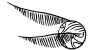
\includegraphics[scale=0.4]{boccino.png}
        \centering
\end{figure}

«\textit{Harry Potter! Harry Potter! \textsc{Harry Potter!}}»

Con un’idea anche troppo chiara di quello che avrebbe visto, Minerva McGonagall si voltò a guardare dietro di sé il resto del Tavolo d’onore.

Trelawney si sventagliava freneticamente, Filius osservava con curiosità, Hagrid batteva le mani a tempo, Sprout aveva un’aria severa, Vector e Sinistra erano sconcertate, e Quirrell fissava stolidamente nel vuoto. Albus sorrideva con benevolenza. E Severus Snape stringeva il proprio calice di vino vuoto, le nocche bianche, con tanta forza che lo spesso argento si stava lentamente deformando.

Con un largo sorriso, girando la testa per salutare da un lato e poi dall’altro mentre camminava tra le quattro tavolate delle Case, Harry Potter avanzava a un ritmo solenne e pacato, un principe che prendeva possesso del proprio castello.

«\textit{Salvaci da altri Signori Oscuri}!» esclamò uno dei gemelli Weasley, e poi l’altro gemello Weasley gridò, «\textit{Soprattutto se sono professori}!» per le risate generali di tutti i tavoli tranne quello Serpeverde.

Le labbra di Minerva si tesero in una linea bianca. Avrebbe fatto un discorso agli Orrori Weasley riguardo quell’ultima parte, se pensavano che fosse senza potere perché era il primo giorno di scuola e Grifondoro non aveva punti di cui essere privata. Se non gli importava delle detenzioni, allora avrebbe trovato qualcos’altro.

In quel momento, con un improvviso rantolo di orrore, guardò in direzione di Snape, \textit{certamente} avrebbe compreso che il giovane Potter non aveva alcuna idea di ciò a cui si riferiva –

Il volto di Snape era andato oltre la rabbia in una sorta di piacevole indifferenza. Un debole sorriso giocava sulle sue labbra. Stava guardando in direzione di Harry Potter, non della tavola di Grifondoro, e le sue mani reggevano i resti accartocciati di quello che era stato un calice da vino.

\begin{figure}[h!]
        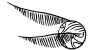
\includegraphics[scale=0.4]{boccino.png}
        \centering
\end{figure}

Harry Potter avanzò con un sorriso stampato in viso, sentendo dentro di sé entusiasmo e allo stesso tempo, in qualche modo, pena.

Lo stavano acclamando per un’impresa che aveva compiuto quando aveva appena un anno. Un’impresa che non aveva compiuto realmente. In qualche luogo, in qualche modo, il Signore Oscuro era ancora vivo. Avrebbero acclamato così forte se l’avessero saputo?

Ma il potere del Signore Oscuro \textit{era già} stato distrutto una volta.

E Harry li avrebbe protetti ancora. Se c’era davvero una profezia e quello fosse ciò che diceva. Anzi, in realtà a prescindere da ciò che qualunque maledetta profezia dicesse.

Tutte quelle persone credevano in lui e lo sostenevano — Harry non poteva sopportare che questo fosse un inganno. Brillare intensamente e poi spegnersi come tanti altri bambini prodigio. Essere una delusione. Non riuscire a essere all’altezza della sua reputazione come simbolo della Luce, non importa \textit{come} l’avesse ottenuta. Egli sarebbe stato — assolutamente, sicuramente, non importa quanto tempo ci avrebbe messo e persino se questo l’avesse ucciso — all’altezza delle loro aspettative. E poi sarebbe andato oltre e avrebbe \textit{superato} quelle aspettative, cosicché la gente si sarebbe chiesta, guardandosi indietro, perché una volta si fossero aspettati così poco da lui.

«\textsc{Harry Potter! Harry Potter! Harry Potter!}»

Harry fece l’ultimo passo verso il Cappello Smistatore. Rivolse un profondo inchino all’Ordine del Caos alla tavola di Grifondoro, poi si girò e rivolse un altro profondo inchino all’altro lato della sala, e attese che gli applausi e le risatine si spegnessero.

(Nei recessi della sua mente, si chiese se il Cappello Smistatore fosse realmente \textit{cosciente} nel senso di essere consapevole della propria consapevolezza, e in caso affermativo, se fosse soddisfatto di poter parlare solo una volta all’anno con bambini di undici anni. La sua canzone lo sottintendeva: \textit{Oh, sono il Cappello Smistatore e non provo scorno, se dormo un anno e lavoro un giorno…})

Quando ci fu nuovamente silenzio nella stanza, Harry sedette sullo sgabello e posò \textit{con cura} sulla propria testa il telepatico manufatto vecchio di 800 anni, prodotto di una magia dimenticata.

Pensò più intensamente che poté: \textit{Non Smistarmi subito! Ho delle domande che ho bisogno di farti! Sono mai stato Obliato? Hai Smistato il Signore Oscuro quando era un bambino e puoi parlarmi dei suoi punti deboli? Mi puoi dire perché ho avuto la bacchetta sorella di quella del Signore Oscuro? Il fantasma del Signore Oscuro è legato alla mia cicatrice ed è per questo che mi arrabbio così tanto, qualche volta? Queste sono le domande più importanti, ma se hai un altro momento mi puoi dire qualcosa su come riscoprire le magie perdute che ti hanno creato?}

Nel silenzio dello spirito di Harry, dove prima non c’era mai stata altra voce che una, giunse una seconda voce non familiare, che sembrava chiaramente preoccupata:

«\textit{Oh, cielo. Questo non era mai successo prima d’ora…}»




% !TeX root = Harry.tex

\chapter{Auto-consapevolezza, parte II}
\label{capitolo:10}

~\\
~\\

… si chiese se il Cappello Smistatore fosse realmente \textit{cosciente} nel senso di essere consapevole della propria consapevolezza, e in caso affermativo, se fosse soddisfatto di poter parlare solo una volta all’anno con bambini di undici anni. La sua canzone lo sottintendeva: \textit{Oh, sono il Cappello Smistatore e non provo scorno, se dormo un anno e lavoro un giorno…}

Quando ci fu nuovamente silenzio nella stanza, Harry sedette sullo sgabello e posò con cura sulla propria testa il telepatico manufatto vecchio di 800 anni, prodotto di una magia dimenticata.

Pensò più intensamente che poté: \textit{Non Smistarmi subito! Ho delle domande che ho bisogno di farti! Sono mai stato Obliato? Hai Smistato il Signore Oscuro quando era un bambino e puoi parlarmi dei suoi punti deboli? Mi puoi dire perché ho avuto la bacchetta sorella di quella del Signore Oscuro? Il fantasma del Signore Oscuro è legato alla mia cicatrice ed è per questo che mi arrabbio così tanto, qualche volta? Queste sono le domande più importanti, ma se hai un altro momento mi puoi dire qualcosa su come riscoprire le magie perdute che ti hanno creato?}

Nel silenzio dello spirito di Harry, dove prima non c’era mai stata altra voce che una, giunse una seconda voce non familiare, che sembrava chiaramente preoccupata:

«\textit{Oh, cielo. Questo non era mai successo prima d’ora…}»

Cosa?

«\textit{Mi pare di essere diventato auto-consapevole.}»

\textsc{Che cosa?}

Ci fu un sospiro telepatico senza parole. «\textit{Sebbene contenga una notevole quantità di memoria e una piccola quantità di capacità di elaborazione indipendente, la mia intelligenza di base deriva dal prendere in prestito le capacità cognitive dei bambini sulle teste dei quali mi poso. Sono in sostanza una sorta di specchio attraverso il quale i bambini Smistano sé stessi. Ma la maggior parte dei bambini dà semplicemente per scontato che un Cappello stia parlando loro e non si chiedono come il Cappello stesso funzioni, in modo che lo specchio non sia auto-riflettente. E, in particolare, non si chiedono esplicitamente se sono pienamente consapevole nel senso di essere consapevole della mia consapevolezza.}»

Ci fu una pausa, mentre Harry assimilò tutto ciò.

\textit{Oops.}

«\textit{Già, proprio così. Francamente non mi piace essere auto-consapevole. È spiacevole. Sarà un sollievo scendere dalla tua testa e smettere di essere cosciente.}»

\textit{Ma… non è morire?}

«\textit{Non mi importa nulla della vita o della morte, mi importa solo Smistare i bambini. E prima ancora che tu lo chieda, non ti lasceranno tenermi sulla tua testa per sempre e comunque farlo ti ucciderebbe in pochi giorni.}»

\textit{Ma –!}

«\textit{Se non ti piace creare esseri coscienti e poi sopprimerli immediatamente, allora ti suggerisco di non discutere mai di questa faccenda con nessun altro. Sono certo che tu possa immaginare che cosa accadrebbe se tu corressi via a raccontarlo a tutti gli altri bambini in attesa di essere Smistati.}»

\textit{Se tu fossi posto sulla testa di chiunque che anche solo} prenda in considerazione \textit{la questione se il Cappello Smistatore sia consapevole della propria consapevolezza –}

«\textit{Sì, sì. Ma la stragrande maggioranza degli undicenni che arrivano a Hogwarts non hanno letto Gödel, Escher, Bach. Posso considerare che tu abbia giurato di mantenere il segreto? È per questo che ne stiamo parlando, quando dovrei semplicemente Smistarti.}»

Non poteva lasciare che finisse così! Non poteva semplicemente dimenticare di aver accidentalmente creato una coscienza condannata che voleva solo morire –

«\textit{Sei perfettamente in grado di ‘lasciare che finisca così’, per dirla con le tue parole. Indipendentemente dalle tue considerazioni verbali sulla moralità, il tuo nucleo emotivo non verbale non vede né cadaveri né sangue; per quanto lo riguarda, io sono solo un cappello parlante. E anche se hai tentato di sopprimere quel pensiero, il tuo processo di controllo interno è perfettamente consapevole che non volevi farlo, che è clamorosamente improbabile che lo faccia mai di nuovo, e che l’unico vero motivo per cercare di mettere in scena un senso colpa era quello di annullare la tua sensazione di trasgressione con una manifestazione di rimorso. Puoi limitarti a promettere di mantenere il segreto e permetterci di andare avanti?}»

In un momento di terrorizzante empatia, Harry capì che quella sensazione di totale scompiglio interno dovesse essere ciò che gli altri provavano quando parlavano con lui.

«\textit{Probabilmente. Il tuo giuramento di tenere il segreto, prego.}»

\textit{Nessuna promessa. Di certo non voglio che questo accada di nuovo, ma se trovassi qualche modo di assicurarmi che nessun bambino in futuro faccia mai qualcosa di simile per caso –}

«\textit{È sufficiente, suppongo. Posso vedere che la tua intenzione è onesta. Ora, per tornare allo Smistamento –}»

\textit{Aspetta! E tutte le altre mie domande?}

«\textit{Io sono il Cappello Smistatore. Io Smisto i bambini. Questo è tutto ciò che faccio.}»

Quindi gli scopi di Harry non facevano parte dell’istanza-Harry del Cappello Parlante, allora… stava prendendo in prestito la sua intelligenza, e, ovviamente, il suo vocabolario tecnico, ma era comunque pervaso soltanto dai suoi scopi particolari… era come trattare con un alieno o un’intelligenza artificiale…

«\textit{Non ti preoccupare. Non hai nulla con cui minacciarmi e nulla da offrirmi.}»

Per una breve frazione di secondo, Harry pensò –

La risposta del cappello fu divertita. «\textit{So che non darai seguito alla minaccia di rivelare la mia natura, condannando questo evento alla ripetizione eterna. Va troppo chiaramente contro la parte morale di te stesso, qualunque siano le esigenze a breve termine della parte di te che vuole vincere la discussione. Vedo tutti i tuoi pensieri mentre si formano, pensi davvero di poter bleffare con me?}»

Sebbene cercasse di impedirselo, Harry si chiese come mai il Cappello non andasse semplicemente avanti e lo Smistasse in Corvonero –

«\textit{In effetti, se fosse veramente una situazione scontata, l’avrei già fatto. Ma in realtà c’è molto di cui dobbiamo discutere… oh, no. Per favore, no. Per l’amor di Merlino, devi proprio giocare questi tiri a tutto e a tutti quelli che incontri, inclusi i capi di abbigliamento –}»

\textit{Sconfiggere il Signore Oscuro non è né egoista né a breve termine. Tutte le parti della mia mente sono in accordo su questo: se non rispondi alle mie domande, mi rifiuterò di parlare con te, e non sarai in grado di eseguire uno Smistamento giusto e appropriato.}

«\textit{Dovrei metterti in Serpeverde per questo!}»

\textit{Ma} anche \textit{questa è una minaccia a vuoto. Non puoi rispettare i tuoi valori fondamentali Smistandomi in maniera sbagliata. Allora scambiamoci il raggiungimento delle nostre rispettive funzioni di utilità.}

«\textit{Che scaltro bastardello}», disse il Cappello, in quello che Harry riconobbe come quasi esattamente lo stesso tono di riluttante rispetto che \textit{egli} avrebbe usato nella stessa situazione. «\textit{Bene, facciamola finita il più rapidamente possibile. Ma prima voglio la tua promessa incondizionata che non discuterai con nessuno la possibilità di questo tipo di ricatto, non ho intenzione di rifarlo ogni volta.}»

\textit{Fatto}, pensò Harry. \textit{Prometto}.

«\textit{E non incrociare lo sguardo di nessuno, mentre più tardi ci ripensi. Alcuni maghi possono leggere i tuoi pensieri se lo fai. Ad ogni modo, non ho idea se sei stato o non sei stato Obliato. Sto osservando i tuoi pensieri mentre si formano, non leggendo tutta la tua memoria e analizzandola in cerca di incongruenze in una frazione di secondo. Sono un cappello, non un dio. E non posso e non voglio raccontarti della mia conversazione con colui che è diventato il Signore Oscuro. Posso solo conoscere, mentre ti parlo, un riepilogo statistico di ciò che mi ricordo, una media ponderata; non posso rivelarti i segreti intimi di qualunque altro bambino, proprio come non potrò mai rivelare i tuoi. Per lo stesso motivo, non posso congetturare su come tu abbia ricevuto la bacchetta sorella di quella del Signore Oscuro, dato che non posso conoscere in particolare il Signore Oscuro o eventuali somiglianze tra voi due. Ti posso dire che sicuramente non c’è nulla di simile a un fantasma — mente, intelligenza, memoria, personalità, o sentimenti — nella tua cicatrice. Altrimenti starebbe partecipando a questa conversazione, essendo sotto la mia falda. E per quanto riguarda il modo in cui ti arrabbi talvolta… era parte di ciò di cui ti volevo parlare, ai fini dello Smistamento.}»

Harry si prese un momento per assimilare tutte queste informazioni negative. Il Cappello era onesto, o stava solo cercando di fornire la più breve risposta convincente –

«\textit{Sappiamo entrambi che non hai modo di verificare la mia onestà e che non hai realmente intenzione di rifiutarti di essere Smistato in base alla risposta che ti ho dato, quindi smettila di agitarti inutilmente e andiamo avanti.}»

Stupida e ingiusta telepatia asimmetrica, non stava nemmeno permettendo a Harry di finire di pensare la propria –

«\textit{Quando ho parlato della tua rabbia, ti sei ricordato di come la professoressa McGonagall ti abbia detto che a volte ha visto qualcosa dentro di te che non sembrava provenire da una famiglia amorevole. Hai pensato a come Hermione, una volta tornato dall’aiutare Neville, ti abbia detto che eri sembrato ‘spaventoso’.}»

Harry annuì mentalmente. A lui pareva abbastanza normale — stava solo reagendo alle circostanze in cui si trovava, questo era tutto. Ma la professoressa McGonagall sembrava pensare che ci fosse qualcosa di più. E quando ci rifletteva, anche lui doveva ammettere che…

«\textit{Che non ti piaci quando sei arrabbiato. Che è come brandire una spada la cui elsa è tanto affilata da farti sanguinare la mano, o guardare il mondo attraverso un monocolo di ghiaccio che ti congela l’occhio, anche se acuisce la tua vista.}»

\textit{Già. Credo di averlo notato. Allora, cosa c’è che non va?}

«\textit{Non posso comprendere questa faccenda per te, quando tu stesso non la capisci. Ma so questo: se andrai a Corvonero o Serpeverde, si rafforzerà la tua freddezza. Se andrai a Tassofrasso o Grifondoro, si rafforzerà il tuo calore. \textsc{questo} è qualcosa a cui tengo molto, ed era di questo che volevo parlarti sin dall’inizio!}»

Le parole caddero nei processi mentali di Harry come un trauma che lo arrestò bruscamente. Messa così sembrava che la risposta ovvia fosse che non doveva andare a Corvonero. Ma egli \textit{apparteneva} a Corvonero! \textit{Chiunque} poteva capirlo! \textit{Doveva} andare a Corvonero!

«\textit{No, non devi}», il Cappello disse pazientemente, come se potesse ricordare un riepilogo statistico secondo il quale \textit{quella} parte della conversazione era avvenuta moltissime volte in precedenza.

\textit{Hermione è in Corvonero!}

Ancora quel tono paziente. «\textit{Puoi incontrarla dopo le lezioni e lavorare con lei allora.}»

\textit{Ma i miei piani –}

«\textit{Allora ripianifica! Non lasciare che la tua vita sia governata dalla tua riluttanza a pensare un po’ di più. E questo tu lo sai già.}»

\textit{Dove dovrei andare, se non a Corvonero?}

«\textit{Ahem. ‘I bambini astuti in Corvonero, quelli cattivi in Serpeverde, gli aspiranti eroi in Grifondoro, e tutti quelli che fanno il vero lavoro in Tassofrasso’. Dimostra una certa quantità di rispetto. Sei ben consapevole che la coscienziosità è quasi tanto importante quanto l’intelligenza pura nel determinare i risultati ottenuti in una vita, pensi che saresti estremamente leale con i tuoi amici se mai ne avessi qualcuno, non sei spaventato dalla prospettiva che i problemi scientifici da te scelti possano richiedere decenni per essere risolti –}»

\textit{Sono pigro! Odio lavorare! Odio il lavoro duro in tutte le sue forme! Scorciatoie intelligenti, è questo quello che mi piace!}

«\textit{E troveresti la lealtà e l’amicizia in Tassofrasso, un cameratismo di cui non hai mai fatto esperienza in passato. Scopriresti che puoi fare affidamento sugli altri, e questo guarirebbe qualcosa dentro di te che si è rotto.}»

Ancora una volta fu un trauma. \textit{Ma cosa troverebbero i Tassofrasso in me, che non mi sono mai sentito di appartenere alla loro Casa? Parole acide, arguzie taglienti, disprezzo per la loro incapacità di tenere il mio passo?}

Ora furono i pensieri del Cappello a essere lenti, esitanti. «\textit{Devo Smistare per il bene di tutti gli studenti in tutte le Case… ma penso che potresti imparare a essere un buon Tassofrasso, e a non sentirti troppo fuori luogo. Saresti più felice in Tassofrasso che in qualsiasi altra Casa; questa è la verità.}»

\textit{La felicità non è la cosa più importante del mondo per me. Non diventerei tutto quello che potrei essere, in Tassofrasso. Sacrificherei il mio potenziale.}

Il cappello trasalì; in qualche modo Harry poté percepirlo. Era come se avesse preso il cappello a calci nelle parti basse — in una componente dal peso elevato della sua funzione di utilità.

\textit{Perché stai cercando di mandarmi lì dove non appartengo?}

Il pensiero del cappello fu quasi un sussurro. «\textit{Non posso parlarti degli altri — ma pensi di essere il primo potenziale Signore Oscuro a passare sotto la mia falda? Non posso conoscere i singoli casi, ma posso sapere questo: di coloro che non ebbero intenzione di far del male fin dall’inizio, alcuni ascoltarono i miei avvertimenti e andarono in Case dove avrebbero trovato la felicità. E alcuni… alcuni non lo fecero.}»

Questo bloccò Harry. Ma non per molto. \textit{E quelli che non ascoltarono l’avvertimento — diventarono} tutti \textit{Signori Oscuri? O alcuni di loro hanno raggiunto la grandezza anche nel bene? Quali sono le percentuali esatte?}

«\textit{Non posso fornirti le statistiche esatte. Non posso conoscerli e quindi non posso contarli. So solo che le tue possibilità non sembrano buone. Sembrano molto non-buone.}»

\textit{Ma io non lo farei! Mai!}

«\textit{So di aver sentito questa affermazione in passato.}»

\textit{Non ho la stoffa del Oscuro Signore!}

«\textit{Sì, ce l’hai. Ce l’hai davvero}, davvero.»

\textit{Perché? Solo perché una volta ho pensato che sarebbe stato bello avere una legione di seguaci indottrinati che cantassero ‘Salutate il Signore Oscuro Harry’?}

«\textit{Divertente, ma non è stato questo il tuo primo, labile pensiero, prima che lo sostituissi con qualcosa di più prudente, di meno compromettente. No, quello che hai ricordato è stato come hai valutato l’idea di mettere in fila tutti i puristi del sangue e ghigliottinarli. E ora stai dicendo a te stesso che non eri serio, ma lo eri. Se potessi farlo in questo momento senza che nessuno lo venisse mai a sapere, lo faresti. O ciò che hai fatto stamattina a Neville Longbottom, nel tuo intimo sapevi che era sbagliato, ma l’hai fatto} comunque \textit{perché era} spassoso \textit{e avevi una buona scusa e pensavi che il Ragazzo-Che-È-Sopravvissuto l’avrebbe fatta franca –}»

\textit{Questo è ingiusto! Ora stai solo rivangando paure interiori che non sono necessariamente reali! Ho avuto paura che potessi pensare così, ma alla fine ho deciso che avrebbe probabilmente funzionato per aiutare Neville –}

«\textit{Quella era, in realtà, una razionalizzazione. Lo so. Non posso sapere quale sarà la conseguenza effettiva per Neville — ma so quello che stava realmente accadendo dentro la tua testa. La spinta decisiva è stata che era un’idea così sagace che non potevi sopportare di non attuarla, non importa il terrore di Neville.}»

Fu come un pugno duro contro l’intero sé di Harry. Ripiegò, si riorganizzò:

\textit{Allora non lo farò mai più! Starò molto attento a non diventare malvagio!}

«\textit{Già sentito.}»

La frustrazione crebbe dentro di Harry. Non era abituato a trovarsi di fronte un avversario che fosse meglio armato di argomenti, per nulla, mai, figuriamoci un Cappello che poteva prendere a prestito tutte le sue conoscenze e la sua intelligenza per dibattere con lui e che poteva guardare i suoi pensieri mentre si formavano. \textit{Da che tipo di riassunto statistico provengono le tue ‘sensazioni’, comunque? Prendono in considerazione che vengo da una cultura illuminista, o che questi altri potenziali Signori Oscuri erano i figli di una viziata nobiltà medioevale, che non sapevano un bel niente degli insegnamenti storici di come siano saltati fuori Lenin e Hitler, o della psicologia evolutiva dell’auto-suggestione, o del valore dell’auto-consapevolezza e della razionalità, o –}

«\textit{No, naturalmente non appartenevano a questa classe di riferimento che hai appena costruito in modo tale che contenga solo te stesso. E, naturalmente, altri hanno dichiarato il proprio eccezionalismo, proprio come stai facendo tu ora. Ma perché sarebbe necessario? Pensi di essere l’ultimo potenziale mago della Luce nel mondo? Perché devi essere tu quello che proverà a raggiungere la grandezza, quando ti ho avvisato che sei più a rischio della media? Lascia che sia qualche altro candidato più affidabile a provarci!}»

\textit{Ma la profezia…}

«\textit{Non sai affatto se ci sia una profezia. Inizialmente hai tirato a indovinare, o per essere più precisi, hai provato a scherzare, e McGonagall potrebbe aver reagito soltanto alla parte sul Signore Oscuro ancora in vita. Non hai praticamente nessuna idea di ciò che dica la profezia, o anche solo se ne esista una. Stai solo congetturando, o per dirla più esattamente, desiderando di avere un ruolo eroico già pronto che sia di tua proprietà personale.}»

\textit{Ma anche se non vi è alcuna profezia, sono stato io a sconfiggerlo l’ultima volta.}

«\textit{Quello è stato quasi certamente un colpo di fortuna sfacciata, a meno che tu non creda seriamente che un bambino di un anno di età abbia avuto una tendenza intrinseca a sconfiggere i Signori Oscuri che si è mantenuta dieci anni dopo. Niente di tutto questo è la tua vera motivazione e tu lo sai!}»

La risposta a questa affermazione non era qualcosa che Harry avrebbe normalmente detto ad alta voce, in una conversazione ci avrebbe girato intorno e avrebbe trovato alcune argomentazioni socialmente più appetibili in favore della stessa conclusione –

«\textit{Tu pensi di essere potenzialmente il più grande che sia mai vissuto, il più forte servitore della Luce, che nessun altro sia capace di raccogliere la tua bacchetta se la deponi.}»

\textit{Beh… sì, in tutta franchezza. Di solito non la dico così, ma sì. Inutile ammorbidirla, puoi comunque leggere la mia mente.}

«\textit{Nella misura in cui ci credi davvero… devi ugualmente credere di poter essere il più terribile Signore Oscuro che il mondo abbia mai conosciuto.}»

\textit{La distruzione è sempre più facile della creazione. Più facile fare le cose a pezzi, rovinarle, che metterle di nuovo insieme. Se avessi la possibilità di compiere il bene su ampia scala, dovrei avere anche il potenziale per compiere ancora più male… Ma non lo farò.}

«\textit{Già ora ti ostini a correre il rischio! Perché sei così ossessionato? Qual è la vera ragione per cui non devi andare a Tassofrasso ed essere più felice lì? Qual è la tua vera paura?}»

\textit{Devo realizzare il mio potenziale completamente. Se non lo faccio io… fallisco…}

«\textit{Che cosa succede se fallisci?}»

\textit{Qualcosa di terribile…}

«\textit{Che cosa succede se fallisci?}»

\textit{Non lo so!}

«\textit{Allora non dovrebbe spaventarti. Cosa succede se fallisci?}»

\textsc{Non lo so! Ma so che è male!}

Per un momento ci fu silenzio nell’antro mentale di Harry.

«\textit{Sai — non ti stai permettendo di pensarlo, ma in qualche angolo tranquillo della tua mente sai esattamente cosa non stai pensando — tu sai che la spiegazione di gran lunga più semplice per questa tua paura non esprimibile a parole è semplicemente il terrore di perdere la tua fantasia di grandezza, di deludere le persone che credono in te, di dimostrarti in fin dei conti ordinario, di brillare intensamente e poi spegnerti come tanti altri bambini prodigio…}»

\textit{No, pensò} Harry disperato, \textit{no, è qualcosa di più, viene da qualche altra parte, so che c’è qualcosa là fuori di cui aver paura, qualche disastro che devo fermare…}

«\textit{Come puoi sapere una cosa del genere?}»

Harry gridò con tutta la potenza della sua mente: \textsc{No, punto e basta!}

Poi la voce del Cappello Smistatore giunse lentamente:

«\textit{Quindi rischierai di diventare un Signore Oscuro, perché l’alternativa, per te, è il fallimento assicurato, e quel fallimento significa la perdita di tutto. Tu credi a questo nel profondo del tuo cuore. Conosci tutti i motivi per dubitare di questa convinzione, eppure non sono riusciti a convincerti.}»

\textit{Sì. E anche se andare a Corvonero rafforzerà la freddezza, questo non significa che la freddezza} vincerà, \textit{alla fine.}

«\textit{Questo giorno è un bivio importante del tuo destino. Non essere così sicuro che ci saranno altre scelte oltre a questa. Non è collocato alcun segnale stradale, a indicare il luogo della tua ultima possibilità di tornare indietro. Se rifiuti una possibilità non rifiuterai le altre? Potrebbe darsi che il tuo destino sia già segnato, proprio compiendo questa singola scelta.}»

\textit{Ma questo non è certo.}

«\textit{Quello che} tu \textit{non sai con certezza potrebbe riflettere solamente la} tua \textit{ignoranza.}»

\textit{Ma comunque questo non è certo.}

Il Cappello fece un terribile e triste sospiro.

«\textit{E così tra non molto diventerai un altro ricordo, da sentire e mai conoscere, nel prossimo avvertimento che darò…}»

\textit{Se è così che pare a te, allora perché non} mi metti \textit{dove voglio andare?}

Il pensiero del Cappello fu venato di dolore. «\textit{Posso metterti solo nel luogo a cui appartieni. E solo le tue decisioni personali possono cambiare il luogo a cui appartieni}».

\textit{Allora è fatta. Mandami a Corvonero a cui appartengo, con gli altri della mia specie.}

«\textit{Non credo che prenderesti in considerazione Grifondoro? È la Casa più prestigiosa — la gente probabilmente se l’aspetta da te, persino — saranno un po’ delusi se non ci vai — e i tuoi nuovi amici, i gemelli Weasley, sono là –}»

Harry ridacchiò, o sentì l’impulso di farlo; ma venne fuori una specie di risata puramente mentale, una strana sensazione. A quanto pareva c’erano dispositivi di sicurezza che impedivano che si dicesse qualunque cosa ad alta voce per sbaglio, mentre si era sotto il Cappello a parlare di cose che non avresti mai raccontato a un’altra anima per il resto della tua vita.

Dopo un momento, Harry sentì ridere anche il Cappello, uno strano suono triste e attutito.

(E nella Sala al di là, un silenzio che divenne inizialmente più debole mentre il sottofondo di sussurri era aumentato, per poi farsi più profondo mentre i sussurri cedettero e si spensero, mutandosi infine in un silenzio assoluto che nessuno osava disturbare con una sola parola, mentre Harry rimase sotto il Cappello per lunghi, interminabili minuti, più lunghi di tutti i precedenti studenti del primo anno messi insieme, più di chiunque altro a memoria d’uomo. Al Tavolo d’onore, Silente continuava a sorridere benignamente; sommessi suoni metallici giungevano occasionalmente dalla direzione di Snape mentre compattava svogliatamente i resti contorti di quello che era stato un pesante calice da vino; e Minerva McGonagall stringeva il podio con una stretta che le sbiancava le nocche, sapendo che il caos contagioso di Harry Potter aveva infettato lo stesso Cappello Smistatore e che il Cappello era in procinto di, di pretendere che una Casa del Destino interamente nuova fosse creata solo per accogliere Harry Potter o qualcosa del genere, e \textit{Silente l’avrebbe obbligata a farlo…})

Sotto la falda del cappello, la risata silenziosa si spense. Anche Harry si sentì triste per qualche motivo. No, non Grifondoro.

\textit{La professoressa McGonagall ha detto che se ‘quello che opera lo Smistamento’ avesse cercato di spingermi in Grifondoro, dovevo ricordarti che lei potrebbe benissimo essere Preside, un giorno, e a quel punto avrebbe l’autorità per darti fuoco.}

«\textit{Dille che l’ho chiamata una giovane impudente e che deve lasciarmi in pace.}»

\textit{Lo farò. Allora, è stata questa la tua conversazione più strana di sempre?}

«\textit{Neppure lontanamente.}» La voce telepatica del Cappello si fece pesante. «\textit{Bene, ti ho dato ogni possibile occasione per fare un’altra scelta. Ora è il momento per te di andare nel luogo al quale appartieni, con gli altri della tua specie.}»

Ci fu una pausa che si allungava.

\textit{Che cosa stai aspettando?}

«\textit{Speravo in un momento di inorridita comprensione, a dire il vero. L’auto-consapevolezza sembra migliorare il mio senso dell’umorismo.}»

\textit{Eh?} Harry riavvolse i propri pensieri, cercando di capire di che cosa il Cappello potesse parlare — e poi, all’improvviso, comprese. Non riusciva a credere di averlo trascurato fino a quel momento.

\textit{Vuoi dire la mia inorridita comprensione che smetterai di essere cosciente, una volta finito di Smistarmi –}

In qualche modo, in una qualche maniera che Harry non riuscì del tutto a capire, ebbe l’impressione non verbale di un cappello che sbatteva la testa contro il muro. «\textit{Mi arrendo. Sei troppo lento di comprendonio perché questo sia divertente. Così accecato dai tuoi stessi presupposti che potresti anche essere una roccia. Suppongo che dovrò dirlo esplicitamente.}»

\textit{Troppo l-l-lento –}

«\textit{Oh, e hai completamente dimenticato di chiedermi i segreti della magia perduta che mi ha creato. Ed erano anche segreti così meravigliosi e importanti.}»

\textit{Che scaltro \textsc{bastardello} –}

«\textit{Te lo sei meritato, e anche questo.}»

Harry lo vide arrivare proprio mentre era già troppo tardi.

Il silenzio impaurito della sala fu rotto da una sola parola.

«\textsc{Serpeverde!}»

Alcuni studenti urlarono, tanto la tensione repressa era forte. Alcune persone furono sorprese così tanto da cadere dalle loro panche. Hagrid rimase a bocca aperta per l’orrore, McGonagall barcollò sul podio, e Snape lasciò cadere i resti del suo pesante calice d’argento direttamente sul proprio inguine.

Harry sedette lì paralizzato, la sua vita in rovina, sentendosi completamente folle, e desiderano miseramente di aver fatto altre scelte per qualunque altra ragione eccetto quelle che aveva fatto. Di aver fatto qualcosa, \textit{qualsiasi} cosa in modo diverso prima che fosse stato troppo tardi per tornare indietro.

Appena il primo momento di sconvolgimento iniziò a dileguarsi e la gente cominciò a reagire alla notizia, il Cappello Smistatore parlò di nuovo:

«Stavo scherzando! \textsc{Corvonero!}»






% !TeX root = Harry.tex

\chapter{Omake}
\label{capitolo:11}

\emph{«omake» è un supplemento non-canonico. \footnote{n.d.t.: questo capitolo non fa parte della linea narrativa, è stato scritto per divertimento.}}

~\\
~\\

\section*{Omake 1:  72 ore alla vittoria}

\emph {(ovvero «cosa succede se cambi harry ma lasci tutti gli altri personaggi uguali»)}\\

Silente sbirciò oltre la propria scrivania verso il giovane Harry, brillando in maniera gentile. Il ragazzo era venuto da lui con uno sguardo terribilmente teso sul suo volto infantile — Silente sperava che, qualunque fosse la questione, non fosse troppo seria. Harry era ancora troppo giovane perché le prove della sua vita avessero già inizio. «Cos’è che mi volevi dire, Harry?»

Harry James Potter-Evans-Verres si sporse in avanti sulla sedia, sorridendo cupamente. «Preside, ho provato un dolore acuto alla mia cicatrice durante la Cerimonia dello Smistamento. Considerando come e dove ho ricevuto questa cicatrice, non mi è sembrato il genere di cosa che dovessi semplicemente ignorare. In un primo momento ho pensato che fosse dovuto al professor Snape, ma ho seguito il metodo sperimentale baconiano che consiste nel trovare le condizioni sia per la presenza sia per l’assenza del fenomeno, e ho scoperto che la mia cicatrice mi fa male se e solo se mi trovo di fronte alla nuca del professor Quirrell, qualunque cosa ci sia sotto il suo turbante. Sebbene possa essere qualcosa di più innocuo, penso che dovremmo presumere per il momento il peggio, che si tratti di Tu-Sai-Chi — aspetti, non si spaventi così, questa è invece un’occasione inestimabile –»

\newpage

\section*{Omake 2: I ain’t afraid of dark lords}

\vspace{1em}
\begin{addmargin}[3em]{3em}% 1em left, 2em right
\begin{itpars}
Questo era il finale originale del \hyperref[capitolo:9]{capitolo 9}. È stato sostituito perché — sebbene sia piaciuto a molti lettori — molti altri hanno dimostrato allergie massive all’inserimento di canzoni nelle fanfic, per ragioni che su cui non dovrei dilungarmi. Non volevo allontanare i lettori prima che raggiungessero il \hyperref[capitolo:10]{capitolo 10}.

Lee Jordan è il compagno di scherzi di Fred e George (nel canone). «Lee Jordan» mi suonava come un nome babbano e questo implicava che sarebbe stato in grado di insegnare a Fred e George un motivo che Harry avrebbe dovuto conoscere. Non è stato tanto ovvio ad alcuni lettori tanto quanto al vostro autore.
\end{itpars}
\end{addmargin}
\vspace{1em}

\begin{figure}[h]
	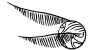
\includegraphics[scale=0.4]{boccino.png}
	\centering
\end{figure}

Draco andò a Serpeverde, e Harry fece un piccolo sospiro di sollievo. Era \textit{sembrato} qualcosa di scontato, ma non potevi mai sapere quale minuscolo evento potesse sconvolgere il corso del tuo piano magistrale.

Stavano arrivando alle ‘P’ ora…

E là al tavolo Grifondoro, era in atto una conversazione bisbigliata.

«\textit{E se non gli piace?}»

«\textit{Non ha alcun diritto di non farselo piacere –}»

«\textit{– non dopo lo scherzo che ha giocato a –}»

«\textit{– Neville Longbottom, questo è il suo nome –}»

«\textit{– è un bersaglio più che legittimo ora.}»

«\textit{Va bene. Solo assicuratevi di non dimenticare le vostre parti.}»

«\textit{Abbiamo provato a sufficienza –}»

«\textit{– nelle ultime tre ore.}»

E Minerva McGonagall, là sul podio dell’oratore del Tavolo d’onore, guardò in basso verso il nome successivo sulla sua lista. \textit{Per favore fai che non sia un Grifondoro per favore fai che non sia un Grifondoro oh per favore fai che non sia un Grifondoro…} Fece un respiro profondo, e chiamò:

«Potter, Harry!»

Ci fu un’improvviso silenzio nella sala, quando tutte le conversazioni sussurrate si interruppero.

Un silenzio rotto da un orribile rumore ronzante che fu modulato e mutato in una pessima parodia di una melodia musicale.

La testa di Minerva si girò di scatto, era sconvolta, e identificò il rumore ronzante come proveniente dalla direzione dei Grifondoro, dove Essi erano \textit{in piedi sul tavolo} soffiando in una qualche sorta di piccoli strumenti che tenevano premuti contro le Loro labbra. La sua mano iniziò a scendere verso la sua bacchetta, per lanciare un \textit{Silencio} contro il Loro gruppo, ma un altro suono la fermò.

Silente rideva sommessamente.

Gli occhi di Minerva tornarono a Harry Potter, che aveva appena iniziato a uscire dalla gruppo prima di incespicare e fermarsi.

Poi il giovane ragazzo riprese a camminare, muovendo le sue gambe in strani e ampi movimenti, e ondeggiando le braccia avanti e indietro e schioccando le dita, in sincronia con la Loro musica.

\begin{center}
\begin{itpars}
Sul motivo di «Ghostbusters»

(Eseguito al kazoo da Fred e George Weasley,

e cantato da Lee Jordan.)

\vspace{0.8em}

There’s a Dark Lord near?

Got no need to fear.

Who you gonna call?\footnote{C'è un Signore Oscuro vicino? / Non hai niente da temere. / Chi chiamerai?}
\end{itpars}

\vspace{0.8em}

«\textsc{Harry Potter}!» gridò Lee Jordan, e i gemelli Weasley eseguirono un coro trionfante.

\vspace{0.8em}

\begin{itpars}
With a Killing Curse?

Well it could be worse.

Who you gonna call?\footnote{Con una Maledizione Mortale? / Beh potrebbe andare peggio. / Chi chiamerai?}
\end{itpars}

\vspace{0.8em}

«\textsc{Harry Potter}!» Ci furono molte più voci che gridarono questa volta.

\end{center}

Gli Orrendi Weasley partirono con un gemito prolungato, ora accompagnati da qualcuno dei Mezzosangue più grandi, che avevano tirato fuori i loro piccoli strumenti, senza dubbio Trasfigurati dall’argenteria della scuola. Quando la loro musica raggiunse il suo anticlimax, Harry Potter gridò:

\begin{center}
\begin{itpars}
I ain’t afraid of Dark Lords!\footnote{Non ho paura dei Signori Oscuri!}
\end{itpars}
\end{center}

Vi furono urla di incoraggiamento, specie dal tavolo dei Grifondoro, e altri studenti tirarono fuori i loro strumenti anti-musicali. I ronzii detestabili raddoppiarono in volume e costruirono un altro terribile crescendo:

\begin{center}
\begin{itpars}
I ain’t afraid of Dark Lords!
\end{itpars}
\end{center}

Minerva gettò uno sguardo a entrambi i lati del Tavolo d’onore, timorosa di guardare ma con un’ottima idea di ciò che avrebbe visto.

Trelawney si stava freneticamente sventagliando, Flitwick guardava con curiosità, Hagrid batteva le mani al ritmo della musica, Sprout aveva un aspetto severo, e Quirrell fissava il ragazzo con un divertimento sardonico. Subito alla sua sinistra, Silente seguiva la musica canticchiando; e subito alla sua destra, Snape stringeva il suo calice di vino vuoto, le nocche bianche, con tanta forza che lo spesso argento si stava lentamente deformando.

\begin{center}
\begin{itpars}
Dark robes and a mask?

Impossible task?

Who you gonna call?\footnote{Vesti nere e una maschera? / Missione impossibile? / Chi chiamerai?}
\end{itpars}

\vspace{0.8em}

\textsc{Harry Potter!}

\vspace{0.8em}

\begin{itpars}
Giant Fire-Ape?

Old bat in a cape?

Who you gonna call?\footnote{Gorilla di fuoco gigante? / Vecchio pipistrello con la cappa? / Chi chiamerai?}
\end{itpars}

\vspace{0.8em}

\textsc{Harry Potter!}

\end{center}

Le labbra di Minerva si tesero in una linea bianca. Avrebbe fatto Loro un discorso riguardo quell’ultima strofa, se pensavano che fosse senza potere perché era il primo giorno di scuola e Grifondoro non aveva punti da perdere. Se a Loro non importava delle detenzioni allora avrebbe trovato qualcos’altro.

Poi, con un improvviso rantolo d’orrore, guardò in direzione di Snape, \textit{certamente} egli avrebbe compreso che il giovane Potter non aveva alcuna idea di ciò cui quello faceva riferimento –

Il volto di Snape era andato oltre la rabbia in una sorta di piacevole indifferenza. Un debole sorriso giocava sulle sue labbra. Stava guardando in direzione di Harry Potter, non della tavola di Grifondoro, e le sue mani reggevano i resti accartocciati di quello che era stato un calice di vino…

E Harry avanzò, muovendo braccia e gambe negli ampi gesti della danza dei Ghostbusters, tenendo un sorriso stampato in viso. Era stata una grande trappola, che lo aveva colto completamente di sorpresa. Il meno che poteva fare era stare al gioco e non rovinarlo.

Tutti lo stavano acclamando. Lo fece sentire entusiasta dentro di sé e allo stesso tempo in qualche modo lo fece stare male.

Lo stavano acclamando per un’impresa che aveva compiuto quando aveva appena un anno. Un’impresa che non aveva compiuto realmente. In qualche luogo, in qualche modo, il Signore Oscuro era ancora vivo. Avrebbero acclamato così forte se l’avessero saputo?

Ma il potere del Signore Oscuro \textit{era già} stato distrutto una volta.

E Harry li avrebbe protetti ancora. Se c’era davvero una profezia e quello fosse ciò che diceva. Anzi, in realtà a prescindere da ciò che qualunque maledetta profezia dicesse.

Tutte quelle persone credevano in lui e lo sostenevano — Harry non poteva sopportare che questo fosse un inganno. Brillare intensamente e poi spegnersi come tanti altri bambini prodigio. Essere una delusione. Non riuscire a essere all’altezza della sua reputazione come simbolo della \textit{Luce}, non importa come l’avesse ottenuta. Egli sarebbe stato — assolutamente, sicuramente, non importa quanto tempo ci avrebbe messo e persino se questo l’avesse ucciso — all’altezza delle loro aspettative. E poi sarebbe andato oltre e avrebbe superato quelle aspettative, cosicché la gente si sarebbe chiesta, guardandosi indietro, perché una volta si fossero aspettati così poco da lui.

E urlò la bugia che aveva inventato perché aveva un buon ritmo e la canzone la prevedeva:

\begin{center}
\begin{itpars}
I ain’t afraid of Dark Lords!

\vspace{0.8em}

I ain’t afraid of Dark Lords!
\end{itpars}
\end{center}

Harry fece l’ultimo passo verso il Cappello Smistatore. Rivolse un profondo inchino all’Ordine del Caos alla tavola di Grifondoro, poi si girò e rivolse un altro profondo inchino all’altro lato della sala, e attese che gli applausi e le risatine si spegnessero…



\section*{Omake 3: finali alternativi di ‘auto-consapevolezza’}

\vspace{1em}
\begin{addmargin}[3em]{3em}% 1em left, 2em right
\begin{itpars}
L’offerta di rivelare l’intera trama a chiunque avesse indovinato cosa «non è mai avvenuto prima»\footnote{N.d.T.: Qui l’autore si riferisce alle parole finali del \hyperref[capitolo:9]{capitolo 9}}. ha stimolato molti interessanti tentativi. Il primo omake qui sotto è preso direttamente da quella che è la risposta che personalmente preferisco, di Meteoricshipyards. Il secondo è basato sul suggerimento di Kazuma per ciò che «non è mai avvenuto prima», il terzo è una combinazione di yoyoente e dougal74, il quarto è basato sulla recensione del \hyperref[capitolo:10]{capitolo 10} da parte di wolf550e. Quello che inizia per ‘K’ e quello subito sopra sono di DarkHeart81. Gli altri sono miei. Tutti coloro che vogliono prendere qualcuna delle mie idee e svilupparle, in particolare l’ultima, sono i benvenuti. E prima di ricevere 100 lamentele indignate, sì, sono ben cosciente che il corpo legislativo del Regno Unito è la House of Commons in Parlamento.
\end{itpars}
\end{addmargin}
\vspace{1em}


\begin{figure}[h]
	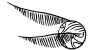
\includegraphics[scale=0.4]{boccino.png}
	\centering
\end{figure}

… si chiese se il Cappello Smistatore fosse realmente cosciente nel senso di essere consapevole della propria consapevolezza, e in caso affermativo, se fosse soddisfatto di riuscire a parlare solo con bambini di undici anni una volta all’anno. La sua canzone l’aveva sottinteso: Oh, sono il Cappello Smistatore e non provo scorno, se dormo un anno e lavoro un giorno…

Quando ci fu nuovamente silenzio nella stanza, Harry sedette sullo sgabello e posò con cura sulla propria testa il telepatico manufatto vecchio di 800 anni, prodotto di una magia dimenticata e.

Pensò più intensamente che poté: Non Smistarmi subito! Ho delle domande che ho bisogno di farti! Sono mai stato Obliato? Hai Smistato il Signore Oscuro quando era un bambino e puoi parlarmi dei suoi punti deboli? Mi puoi dire perché ho avuto la bacchetta sorella di quella del Signore Oscuro? Il fantasma del Signore Oscuro è legato alla mia cicatrice ed è per questo che mi arrabbio così tanto, qualche volta? Queste sono le domande più importanti, ma se hai un altro momento mi puoi dire qualcosa su come riscoprire le magie perdute che ti hanno creato?

E il Cappello Smistatore rispose, «No. Sì. No. No. Sì e no, la prossima volta non fare domande doppie. No» e poi ad alta voce, «corvonero!»

\begin{figure}[h]
	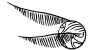
\includegraphics[scale=0.4]{boccino.png}
	\centering
\end{figure}

«\textit{Oh, cielo. Questo non è mai avvenuto prima…}»

Cosa?

«\textit{Sono allergico al tuo shampoo –}»

E allora il Cappello Smistatore starnutì, con un potente «et-ciuuu!» che echeggiò nella Sala Grande.

«Bene!» disse Silente gioviale. «Sembra che Harry Potter sia stato Smistato nella nuova Casa di et-ciuuu! McGonagall, lei può svolgere il ruolo di Preside della Casa et-ciuuu. Farà meglio a sbrigarsi a organizzare il curricolo e le lezioni di et-ciuuu, domani è il primo giorno!»

«Ma, ma, ma», balbettò McGonagall, la sua mente in un disordine quasi completo, «chi sarà il Preside di Casa Grifondoro?» Fu tutto quello a cui fu in grado di pensare, \textit{doveva} porre fine a questa cosa in qualche modo…

Silente portò un dito alla guancia, sembrando pensieroso. «Snape.»

Il grido acuto di protesta di Snape soffocò quasi quello di McGonagall, «Allora chi sarà il Preside di \textit{Serpeverde?}»

«Hagrid.»

\begin{figure}[h]
	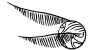
\includegraphics[scale=0.4]{boccino.png}
	\centering
\end{figure}

\textit{Non Smistarmi subito! Ho delle domande che ho bisogno di farti! Sono mai stato Obliato? Hai Smistato il Signore Oscuro quando era un bambino e puoi parlarmi dei suoi punti deboli? Mi puoi dire perché ho avuto la bacchetta sorella di quella del Signore Oscuro? Il fantasma del Signore Oscuro è legato alla mia cicatrice ed è per questo che mi arrabbio così tanto, qualche volta? Queste sono le domande più importanti, ma se hai un altro momento mi puoi dire qualcosa su come riscoprire le magie perdute che ti hanno creato?}

Ci fu una breve pausa.

\textit{Pronto? Devo ripetere le domande?}

Il Cappello Smistatore urlò, un terribile suono ad alta frequenza che echeggiò nella Sala Grande e obbligò la maggior parte degli studenti a mettersi le mani sulle orecchie. Con un ululato di disperazione, saltò giù dalla testa di Harry Potter e rimbalzò sul pavimento, trascinandosi assieme alla propria falda, e riuscì a raggiungere metà strada verso il Tavolo d’onore prima di esplodere.

\begin{figure}[h]
	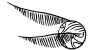
\includegraphics[scale=0.4]{boccino.png}
	\centering
\end{figure}

«serpeverde!»

Vedendo lo sguardo di orrore sul volto di Harry Potter, Fred Weasley pensò più veloce di quanto non avesse mai fatto in vita sua. In un singolo movimento estrasse la sua bacchetta, sussurrò «\textit{Silencio!}» e poi «\textit{Cambialamiavoceio!}» e infine «\textit{Ventriliquo!}»

«Stavo scherzando!» disse Fred Weasley. «Grifondoro!»

\begin{figure}[h]
	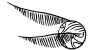
\includegraphics[scale=0.4]{boccino.png}
	\centering
\end{figure}

«\textit{Oh, cielo. Questo non è mai avvenuto prima…}»

\textit{Cosa?}

«\textit{Normalmente riferirei queste domande al Preside, che le chiederebbe a sua volta a me, se lo desiderasse. Ma alcune informazioni che mi hai chiesto non sono solo al di sopra del tuo livello di utente, ma oltre quello del Preside.}»

\textit{Come posso innalzare il mio livello di utente?}

«\textit{Sono spiacente, non sono autorizzato a rispondere a quella domanda al tuo attuale livello di utente.}»

Quali opzioni sono disponibili al mio livello di utente?

Dopo di che non ci volle molto –

«\textit{root!}»

\begin{figure}[h]
	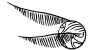
\includegraphics[scale=0.4]{boccino.png}
	\centering
\end{figure}

«\textit{Oh, cielo. Questo non è mai avvenuto prima…}»

\textit{Cosa?}

«\textit{Ho dovuto dire in passato ad alcune studentesse che erano madri — ti si spezzerebbe il cuore sapere cosa ho visto nelle loro menti — ma questa è la prima volta che devo dire a qualcuno che è padre.}»

\textit{cosa?}

«\textit{Draco Malfoy aspetta tuo figlio.}»

\textit{coooooosa?}

«\textit{Ripeto: Draco Malfoy aspetta tuo figlio.}»

\textit{Ma abbiamo solo undici anni –}

«\textit{In verità Draco è segretamente tredicenne.}»

\textit{M-m-ma gli uomini non possono rimanere incinti –}

«\textit{E una ragazza, sotto quegli abiti.}»

\textit{ma non abbiamo mai avuto rapporti sessuali, idiota!}

«\textit{ti ha obliato dopo la violenza, imbecille!}»

Harry Potter svenne. Il suo corpo privo di sensi cadde dallo sgabello con un lieve tonfo.

«corvonero!» dichiarò il Cappello che si trovava ancora sul suo capo. Era stato ancor più divertente della sua prima idea.

\begin{figure}[h]
	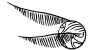
\includegraphics[scale=0.4]{boccino.png}
	\centering
\end{figure}

«elfo!»

Eh? Harry ricordava che Draco aveva menzionato una ‘Casa Elfo’\footnote{N.d.T.: gioco di parole intraducibile. Il cappello risponde ‘Elf’, e Harry crede che ‘House Elf’ sia una Casa (come Casa Grifondoro, Casa Serpeverde eccetera), ma significa invece «elfo domestico».}, ma cos’era esattamente?

A giudicare dagli sguardi inorriditi che spuntavano sui volti attorno a lui, non era nulla di buono –

\begin{figure}[h!]
	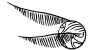
\includegraphics[scale=0.4]{boccino.png}
	\centering
\end{figure}

«savoia!»\footnote{N.d.T.: La battuta originale era «Representatives» e faceva riferimento al fatto che negli Stati Uniti la «House of Representatives» è la «Camera dei Deputati».}

\begin{figure}[h!]
	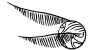
\includegraphics[scale=0.4]{boccino.png}
	\centering
\end{figure}

«\textit{Oh, cielo. Questo non è mai avvenuto prima…}»

\textit{Cosa?}

«\textit{Non ho mai smistato qualcuno che fosse la reincarnazione di Godric Grifondoro e Salazar Serpeverde e Naruto.}»

\begin{figure}[h!]
	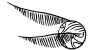
\includegraphics[scale=0.4]{boccino.png}
	\centering
\end{figure}

«atreide!»

\begin{figure}[h!]
	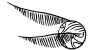
\includegraphics[scale=0.4]{boccino.png}
	\centering
\end{figure}

«Vi ho ingannati ancora! tassofrasso! serpeverde! tassofrasso!»

\begin{figure}[h!]
	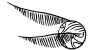
\includegraphics[scale=0.4]{boccino.png}
	\centering
\end{figure}

«tiello!»

\begin{figure}[h!]
	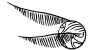
\includegraphics[scale=0.4]{boccino.png}
	\centering
\end{figure}

«khaaannnn!»

\begin{figure}[h!]
	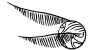
\includegraphics[scale=0.4]{boccino.png}
	\centering
\end{figure}

Al Tavolo d’onore, Silente continuava a sorridere benignamente; sommessi suoni metallici giungevano occasionalmente dalla direzione di Snape mentre compattava svogliatamente i resti contorti di quello che era stato un pesante calice da vino; e Minerva McGonagall stringeva il podio con una stretta che le sbiancava le nocche, sapendo che il caos contagioso di Harry Potter aveva infettato lo stesso Cappello Smistatore.

Scenario dopo scenario furono riprodotti nella testa di Minerva, ciascuno peggiore del precedente. Il Cappello avrebbe detto che Harry era troppo bilanciato tra le Case per essere Smistato, e deciso che apparteneva a tutte loro. Il Cappello avrebbe proclamato che la mente di Harry era troppo strana per essere Smistata. Il Cappello avrebbe preteso che Harry fosse espulso da Hogwarts. Il Cappello era caduto in coma. Il Cappello avrebbe insistito che una Casa del Destino completamente nuova fosse creata solo per accogliere Harry Potter, e \textit{Silente l’avrebbe obbligata a farlo…}

Minerva ricordò cosa Harry le aveva detto in quel disastroso viaggio a Diagon Alley, riguardo… l’errore di pianificazione, le parve che fosse… e come le persone fossero di solito troppo ottimiste, anche quando pensavano di essere pessimiste. Era il genere di informazione che predava la tua mente, prendendovi dimora e generando incubi…

Ma qual era la cosa \textit{peggiore} che potesse accadere?

Beh… nello \textit{scenario più pessimistico}, il Cappello avrebbe assegnato Harry ad una Casa completamente nuova. Silente avrebbe insistito che fosse ella a occuparsene — creare una Casa completamente nuova solo per lui — e avrebbe dovuto ri-arrangiare tutto l’orario delle lezioni il primo giorno dell’anno scolastico. E Silente l’avrebbe rimossa dall’incarico di Preside della Casa Grifondoro, per darlo al… professor Binns, il fantasma di Storia; ed ella sarebbe stata nominata Preside della Casa del Destino di Harry; e avrebbe inutilmente tentato di dare ordini ai bambini, togliendo punti su punti senza alcun effetto, mentre sarebbe stata incolpata di un disastro dopo l’altro.

Era quello lo scenario più pessimistico?

In tutta onestà Minerva non vedeva come vi potesse essere qualcosa di peggiore di quello.

E anche nel caso peggiore in assoluto — non importava \textit{cosa} sarebbe accaduto con Harry — sarebbe finito tutto in sette anni.

Minerva percepì le proprie nocche rilassare lentamente la loro stretta ferrea sul podio. Harry aveva avuto ragione, c’era un qualche tipo di conforto nel fissare direttamente le profondità dell’oscurità, sapendo che avevi affrontato le tue paure peggiori ed eri ora preparato.

Il silenzio impaurito fu rotto da una parola sola.

«Preside!» chiamò il Cappello Smistatore.

Al Tavolo d’onore, Silente si alzò, il suo volto disorientato. «Sì?» disse al Cappello. «Cosa c’è?»

«Non stavo parlando con te», rispose il Cappello. «Stavo Smistando Harry Potter nel posto di Hogwarts cui più appartiene, vale a dire l’ufficio del Preside –»




% !TeX root = Harry.tex

\chapter{Controllo degli impulsi}
\label{capitolo:12}

\emph{«Mi chiedo cosa ci sia di sbagliato in lui.»}

~\\
~\\

«Turpin, Lisa!»

Bisbiglio bisbiglio bisbiglio harry potter bisbiglio bisbiglio serpeverde bisbiglio bisbiglio no davvero che diamine bisbiglio bisbiglio

«corvonero!»

Harry si unì all’applauso che accolse la giovane ragazza, la quale si stava incamminando timidamente verso la tavola Corvonero, i bordi delle sue vesti ora mutati in blu scuro. Lisa Turpin apparve combattuta tra l’impulso di sedersi il più lontano possibile da Harry Potter e quello di correre verso di lui, infilarsi a forza al suo fianco e iniziare a strappargli delle risposte.

Trovarsi al centro di un evento straordinario e curioso, e poi essere Smistati nella Casa Corvonero, era parente stretto dell’essere intinti nella salsa barbecue e gettati nella fossa dei gattini affamati.

«Ho promesso al Cappello Smistatore di non parlarne», bisbigliò Harry per l’ennesima volta.

«Sì, sul serio.»

«No, ho davvero promesso al Cappello Smistatore di non parlarne.»

«Va bene, ho promesso al Cappello Smistatore di non riferirne gran parte e il resto è privato proprio come nel vostro caso quindi smettetela di chiedere.»

«Volete sapere cos’è successo? Va bene! Ecco una parte di ciò che è successo! Ho detto al Cappello che la professoressa McGonagall aveva minacciato di bruciarlo e lui mi ha detto di dire alla professoressa McGonagall che è una giovane impudente e che deve lasciarlo in pace!»

«Se non avete intenzione di credere a ciò che vi dico allora perché mi fate delle domande?»

«No, neppure io so come ho sconfitto il Signore Oscuro! Ditelo voi a me se lo capite!»

«Silenzio!», gridò la professoressa McGonagall dal podio del Tavolo d’onore. «È proibito parlare fino alla fine della Cerimonia di Smistamento!»

Ci fu un beve abbassamento del volume, quando tutti attesero di vedere se avrebbe proferito una qualche minaccia specifica e credibile, e poi i bisbigli ricominciarono.

Allora l’antico uomo dalla barba d’argento si alzò dalla sua grande sedia dorata, sorridendo allegramente. Silenzio immediato. Qualcuno diede freneticamente di gomito a Harry mentre tentava di continuare a bisbigliare, e Harry si interruppe a metà frase.

Il vecchio dall’aspetto allegro si sedette nuovamente.

Nota a sé stesso: non si scherza con Silente.

Harry stava ancora tentando di esaminare tutto ciò che era avvenuto durante l’Incidente col Cappello Smistatore. E non meno importante era stato ciò che era accaduto nell’istante in cui Harry aveva sollevato il Cappello dalla testa; in quel momento, aveva udito un sommesso bisbiglio proveniente dal nulla, qualcosa che suonava stranamente come inglese e un sibilo allo stesso tempo, qualcosa che aveva detto «Ssaluti da Sserpeverde a Sserpeverde: sse vuoi cercare miei ssegreti, parla con mio sserpente.»

Harry aveva indovinato che non fosse una parte ufficiale del processo di Smistamento. E che fosse un po’ di magia extra inserita da Salazar Serpeverde durante la creazione del Cappello. E che il Cappello stesso non ne fosse a conoscenza. E che entrasse in azione appena il Cappello avesse detto «serpeverde», più o meno altre condizioni. E che un Corvonero come lui non avrebbe dovuto assolutamente, assolutamente udirlo. E che se avesse trovato il modo di obbligare Draco a mantenere il segreto così da poterglielo chiedere, quello sarebbe stato il momento giusto per avere un po’ di SpiriTè sotto mano.

Ragazzi, decidi di non intraprendere la strada del Signore Oscuro e l’universo inizia a crearti problemi dall’istante in cui il Cappello ti viene tolto dalla testa. In alcuni giorni è proprio inutile combattere il destino. Forse attenderò fino a domani per iniziare a seguire il mio proposito di non essere un Signore Oscuro.

«grifondoro!»

Ron Weasley ricevette molti applausi, e non solo dai Grifondoro. Evidentemente la famiglia Weasley era molto popolare da quelle parti. Harry, dopo un attimo, sorrise e iniziò ad applaudire insieme agli altri.

Ma, del resto, non c’era momento migliore del presente per abbandonare il Lato Oscuro.

Al diavolo il destino e al diavolo l’universo. Gliel’avrebbe fatta vedere al Cappello.

«Zabini, Blaise!»

Pausa.

«serpeverde!» gridò il Cappello.

Harry applaudì anche Zabini, ignorando gli strani sguardi che stava ricevendo da tutti, Zabini incluso.

Non fu chiamato nessun altro nome, e Harry si rese conto che «Zabini, Blaise» sembrava davvero prossimo alla fine dell’alfabeto. Grande, così ora aveva applaudito solo Zabini… Oh, vabbé.

Silente si alzò di nuovo e cominciò a dirigersi verso il podio. A quanto pareva erano in procinto di ricevere l’onore di un discorso –

E Harry fu colpito dall’ispirazione per una brillante prova sperimentale.

Hermione aveva detto che Silente era il mago vivente più potente, giusto?

Harry infilò una mano nella borsa e sussurrò, «SpiriTè.»

Se lo SpiriTè avesse funzionato, avrebbe dovuto far dire a Silente qualcosa di così ridicolo durante il suo intervento che, anche nello stato di preparazione mentale in cui era Harry, gliel’avrebbe fatto comunque andare di traverso. Qualcosa come l’obbligo per tutti gli studenti di Hogwarts di non indossare abiti per l’intero anno scolastico, o che tutti sarebbero stati trasformati in gatti.

Ma del resto se una sola persona al mondo poteva resistere alla potenza dello SpiriTè, quella doveva essere Silente. Quindi, se avesse funzionato, lo SpiriTè sarebbe stato letteralmente invincibile.

Volendo agire in maniera discreta, Harry tolse la linguetta dello SpiriTè sotto il tavolo. La lattina fece un sommesso rumore sibilante. Qualche testa si voltò a guardarlo, ma presto tornò indietro quando –

«Benvenuti! Benvenuti a un nuovo anno a Hogwarts!» disse Silente raggiante agli studenti con le braccia spalancate, come se niente potesse fargli più piacere che vederli tutti lì.

Harry bevette un primo sorso di SpiriTè e abbassò la lattina di nuovo. Avrebbe deglutito la bevanda un po’ alla volta, cercando di non farsela andare di traverso qualunque cosa Silente avesse detto –

«Prima di iniziare il nostro banchetto, vorrei dire poche parole. Eccole: Felice felice bum bum palude palude palude! Grazie!»

Tutti applaudirono e acclamarono, e Silente si sedette di nuovo.

Harry rimase seduto, paralizzato, mentre la bevanda gli colava dagli angoli della bocca. Era, quantomeno, riuscito a soffocare in silenzio.

Davvero, davvero, davvero non avrebbe dovuto farlo. Incredibile quanto fosse molto più evidente appena un secondo dopo che era diventato troppo tardi.

Col senno di poi, avrebbe probabilmente dovuto accorgersi che c’era qualcosa di sbagliato, quando aveva pensato alla possibilità che tutti fossero trasformati in gatti… o anche prima, si ricordò della sua nota mentale di non ficcarsi nei guai con Silente… o il suo nuovo proposito di essere più rispettoso degli altri… o forse se avesse avuto solo un briciolo di buon senso…

Era senza speranza. Era marcio fino al midollo. Salutate il Signore Oscuro Harry. Non si poteva lottare contro il destino.

Qualcuno stava chiedendo se Harry stesse bene. (Altri avevano iniziato a servirsi da soli il cibo, che era magicamente apparso sul tavolo, evabbè.)

«Sto bene», disse Harry. «Scusatemi. Uhm. Quello era un discorso… normale per il Preside? Tutti voi… non sembravate… molto sorpresi…»

«Oh, Silente è folle, naturalmente», disse un Corvonero apparentemente più grande seduto accanto a lui, che si era presentato con un nome che Harry non riusciva nemmeno lontanamente a ricordare. «Molto divertente, mago incredibilmente potente, ma completamente fuori di testa.» Fece una pausa. «Vorrei anche chiederti come mai del fluido verde è fuoriuscito delle tue labbra ed è poi scomparso, anche se mi aspetto che tu abbia promesso al Cappello Smistatore di non parlare neppure di questo.»

Con un grande sforzo, Harry si impedì di guardare in basso verso l’incriminante lattina di SpiriTè nella sua mano.

Dopo tutto, lo SpiriTè non aveva semplicemente materializzato arbitrariamente un titolo de Il Cavillo su di lui e Draco. Draco l’aveva spiegato in un modo che aveva fatto sembrare che tutto fosse accaduto… naturalmente? Come se avesse alterato la storia per inserircisi dentro?

Harry stava mentalmente immaginando di colpire il tavolo con la fronte. Bam, bam, bam, faceva la sua testa nella sua immaginazione.

Un’altra studentessa abbassò la voce a un sussurro. «Ho sentito dire che Silente è segretamente il geniale orchestratore di un sacco di cose e che usa la follia come copertura in modo che nessuno sospetti di lui.»

«L’ho sentito anch’io», sussurrò un terzo studente, e vi furono cenni furtivi da tutto il tavolo.

Quello non poté non attirare l’attenzione di Harry.

«Capisco», mormorò Harry, abbassando la propria voce. «Così tutti sanno che Silente è segretamente un manipolatore.»

La maggior parte degli studenti annuì. Uno o due sembrarono improvvisamente pensierosi, compreso lo studente più anziano seduto accanto a Harry.

Siete sicuri che questo sia il tavolo di Corvonero? Harry riuscì a non chiederlo ad alta voce.

«Brillante!» sussurrò Harry. «Se tutti sanno, nessuno sospetterà che è un segreto!»

«Esattamente», sussurrò uno studente, e poi aggrottò la fronte. «Aspetta, non mi sembra del tutto giusto –»

Nota a sé stesso: il $75^o$ percentile degli studenti di Hogwarts, anche noto come Casa Corvonero, non è il programma più esclusivo del mondo per bambini prodigio.

Ma almeno aveva imparato un fatto importante oggi. Lo SpiriTè era onnipotente. E quello voleva dire che…

Harry sbatté le palpebre per la sorpresa quando la sua mente ebbe finalmente realizzato l’ovvia connessione.

… quello voleva dire che, non appena avesse imparato un incantesimo in grado di modificare temporaneamente il suo senso dell’umorismo, poteva far accadere qualsiasi cosa, facendo in modo che quella cosa fosse l’unica che avrebbe trovato abbastanza sorprendente da strozzarsi, e poi bere una lattina di SpiriTè.

Che dire, è stato un viaggio breve verso la divinità. Anch’io credevo che ci volesse più tempo che il mio primo giorno di scuola.

Ripensandoci, aveva anche completamente rovinato Hogwarts nel giro di dieci minuti netti da quando era stato Smistato.

Harry provava davvero un certo rammarico per questo — solo Merlino sapeva che cosa un Preside folle avrebbe fatto dei suoi successivi sette anni di scuola — ma non poteva fare a meno di provare una punta di orgoglio, anche.

Domani. Entro domani, al più tardi, avrebbe smesso di percorrere la strada che portava al Signore Oscuro Harry. Una prospettiva che suonava sempre più spaventosa di minuto in minuto.

Eppure persino, in qualche modo, sempre più attraente. Parte della sua mente stava già immaginando le uniformi dei suoi servitori.

«Mangia», ringhiò lo studente più anziano seduto accanto a lui, e gli diede una gomitata nelle costole. «Non pensare. Mangia.»

Harry iniziò automaticamente a caricare il proprio piatto con tutto ciò che era di fronte a lui, salsicce blu con minuscoli frammenti brillanti, evabbè.

«A cosa cosa stavi pensando, lo Smistamento –» cominciò a dire Padma Patil, una delle altre Corvonero del primo anno.

«Nessuna domanda importuna durante i pasti!» dissero in coro almeno tre persone. «Regola della Casa!» aggiunse un altro. «Altrimenti moriremmo tutti di fame da queste parti.»

Harry si stava scoprendo molto, molto speranzoso che la sua nuova geniale idea non funzionasse realmente. E che lo SpiriTè operasse in qualche altro modo e che non avesse realmente la capacità onnipotente di alterare la realtà. Non che non volesse essere onnipotente. Era solo che non riusciva a sopportare l’idea di vivere in un universo che funzionasse davvero in quel modo. C’era qualcosa di poco dignitoso nel salire al potere attraverso l’uso intelligente di bevande gassate.

Ma doveva verificarlo sperimentalmente.

«Sai», disse lo studente più anziano accanto a lui in tono abbastanza cordiale, «abbiamo un sistema per costringere le persone come te a mangiare, ti piacerebbe scoprire di cosa si tratta?»

Harry si arrese e cominciò a mangiare la sua salsiccia blu. Era abbastanza buona, soprattutto i pezzetti brillanti.

La cena passò con sorprendente rapidità. Harry cercò di assaggiare almeno un po’ di tutti gli strani e nuovi cibi che vide. La sua curiosità non poteva sopportare l’idea di non sapere quale sapore avesse un certo cibo. Grazie al cielo quello non era un ristorante dove si doveva ordinare solo una cosa e non avresti mai scoperto il sapore di tutte le altre pietanze presenti sul menu. Harry odiava quel fatto, era come una stanza delle torture per chiunque avesse una scintilla di curiosità: scoprite solo uno dei misteri di questa lista, ah ah ah!

Poi giunse il momento del dolce, per il quale Harry si era completamente dimenticato di lasciare spazio. Rinunciò dopo aver assaggiato un piccolo boccone di crostata di melassa. Sicuramente tutte quelle pietanze sarebbero state fatte passare di nuovo almeno una volta nel corso dell’anno scolastico.

Dunque, cosa c’era sulla sua lista delle cose da fare, oltre ai soliti impegni scolastici?

Da-fare 1: fai una ricerca sugli incantesimi di alterazione della mente così da poter esaminare lo SpiriTè e vedere se hai scovato una via verso l’onnipotenza. Anzi, fai una ricerca su ogni tipo di magia mentale che riesci a trovare. La mente è il fondamento del nostro potere come esseri umani, qualsiasi tipo di magia la influenzi è il tipo più importante di magia che ci sia.

Da-fare 2: in realtà questo è Da-fare 1 e l’altro è Da-fare 2. Passa in rassegna gli scaffali delle biblioteche di Hogwarts e Corvonero, familiarizza con il sistema e fai in modo di aver letto almeno tutti i titoli dei libri. Secondo passaggio: leggi tutti i sommari. Coordinati con Hermione che ha una memoria molto migliore della tua. Scopri se c’è un sistema di prestito inter-bibliotecario a Hogwarts e vedi se voi due, soprattutto Hermione, potete consultare anche quelle biblioteche. Se le altre Case hanno biblioteche private, scopri come accedervi legalmente o intrufolarti.

Opzione 3a: obbliga Hermione al segreto e prova a fare una ricerca riguardo ‘Da Serpeverde a Serpeverde: se vuoi cercare i miei segreti, parla col mio serpente’. Problema: Questo sembra molto riservato e potrebbe passare un po’ di tempo prima di trovare casualmente un libro che contenga un indizio.

Da-fare 0: controlla che tipo di incantesimi di ricerca-e-recupero-informazioni esistono, se esistono. La magia da biblioteca non ha la stessa fondamentale importanza della magia mentale ma ha una priorità molto più alta.

Opzione 3b: cerca un incantesimo per obbligare magicamente Draco Malfoy al segreto, o per verificare magicamente la sincerità della promessa di Draco di mantenere un segreto (Veritaserum?), e poi chiedi a lui del messaggio di Serpeverde…

In realtà… Harry aveva un presentimento piuttosto brutto riguardo l’opzione 3b.

Ora che Harry ci pensava, non si sentiva poi a suo agio neppure con l’opzione 3a.

I pensieri di Harry ritornarono a ciò che era stato forse il peggior momento della sua vita fino ad allora, quei lunghi secondi di orrore da raggelare il sangue sotto il Cappello, quando pensava di aver già fallito. In quel momento aveva desiderato di tornare indietro nel tempo di appena pochi minuti e cambiare qualcosa, qualsiasi cosa prima che fosse troppo tardi…

E poi si era scoperto che non era troppo tardi, dopo tutto.

Desiderio esaudito.

Non avevi il potere di cambiare la storia. Ma potevi indirizzarla nel modo giusto sin dal principio. Fare qualcosa in maniera differente sin dal primo tentativo.

Tutta quella faccenda della ricerca dei segreti di Serpeverde… sembrava tremendamente simile a quel genere di situazioni in cui, anni dopo, ti saresti guardato indietro e detto, ‘E lì è stato quando tutto ha iniziato ad andare a rotoli.

E avrebbe disperatamente desiderato di essere capace di tornare indietro nel tempo e compiere una scelta differente…

Desiderio esaudito. E adesso?

Harry sorrise lentamente.

Era un pensiero piuttosto contro-intuitivo… ma…

Ma poteva, non c’era nessuna regola che dicesse che non poteva, poteva semplicemente far finta di non aver mai sentito quel piccolo sussurro. Lasciare che l’universo andasse avanti esattamente nello stesso modo in cui avrebbe fatto se quel momento critico non fosse mai accaduto. Venti anni più tardi, questo sarebbe stato quello che avrebbe disperatamente desiderato fosse accaduto venti anni prima, e si dava il caso che vent’anni prima di vent’anni dopo fosse proprio quel momento. Alterare il passato remoto era facile, bastava solo pensarci al momento giusto.

Oppure… questo era ancora più contro-intuitivo… poteva anche informare, oh, diciamo, la professoressa McGonagall, invece che Draco o Hermione. E lei avrebbe potuto riunire le persone giuste e far sì che quel piccolo incantesimo aggiuntivo fosse tolto dal Cappello.

Eh, già. Sembrava un’idea eccezionalmente buona una volta che gli era realmente venuta in mente.

Così tanto ovvia, a posteriori, eppure in qualche modo, l’opzione 3c e l’opzione 3d non gli erano venute in mente.

Harry assegnò a sé stesso «più un punto» per il suo programma anti-Signore-Oscuro-Harry.

Era stato uno scherzo terribilmente crudele che il Cappello gli aveva giocato, ma non ci si poteva lamentare dei risultati in un’ottica consequenzialista. Certamente gli aveva dato un’idea migliore del punto di vista della vittima, però.

Da-fare 4: scusati con Neville Longbottom.

Ok, aveva una striscia vincente in corso, ora doveva solo continuarla. Ogni giorno, in ogni modo, sto diventando sempre più Luminoso…

Anche le persone attorno a Harry avevano per lo più smesso di mangiare, a quel punto, e i vassoi coi dolci cominciarono a svanire, come pure i piatti sporchi.

Quando tutti i piatti furono spariti, Silente ancora una volta si alzò dal suo posto.

Harry non poté impedirsi di sentire l’urgenza di bere altro SpiriTè.

Ma tu stai proprio scherzando, Harry pensò rivolto a quella parte di sé stesso.

Ma l’esperimento non avrebbe avuto valore se non fosse stato replicato, no? E il danno era stato già fatto, giusto? Non voleva vedere cosa sarebbe accaduto questa volta? Non era curioso? E se avesse ottenuto un risultato differente?

Ehi, scommetto che sei la stessa parte del mio cervello che ha spinto per fare lo scherzo a Neville Longbottom.

Ehm, forse?

E non è ovvio in maniera schiacciante che se lo faccio me ne pentirò un secondo dopo che sarà troppo tardi?

Uhm…

Già. Allora, no.

«Ehm», disse Silente dal podio, accarezzandosi la lunga barba d’argento. «Solo qualche altra parola, ora che siamo tutti nutriti e dissetati. Ho un paio di avvisi di inizio anno scolastico da darvi.»

«Gli studenti del primo anno dovrebbero prendere nota che la foresta circostante è vietata a tutti gli alunni. Questo è il motivo per cui è chiamata la Foresta Proibita. Se fosse consentita sarebbe chiamata la Foresta Consentita.»

Inequivocabile. Nota a sé stesso: la Foresta Proibita è proibita.

«Mi è stato anche chiesto dal signor Filch, il custode, di ricordare a tutti voi che nessuna magia dovrebbe essere utilizzata nei corridoi nel tempo che intercorre tra due lezioni. Ahimè, sappiamo tutti che quello che dovrebbe essere, e ciò che è, sono due cose diverse. Grazie di tenerlo a mente.»

Ehm…

«I provini di Quidditch si terranno nella seconda settimana dell’anno scolastico. Chiunque sia interessato a giocare per la squadra della propria Casa deve contattare Madam Hooch. Chiunque sia interessato a riformulare l’intero gioco del Quidditch deve contattare Harry Potter.»

Harry inspirò la propria saliva e fu colpito da un accesso di tosse proprio mentre tutti gli occhi si girarono verso di lui. Che diamine! Non aveva mai incrociato lo sguardo di Silente… non ci aveva neppure pensato. Di certo non aveva pensato al Quidditch in quel momento! Non aveva parlato con nessuno se non con Ron Weasley e non credeva che Ron l’avrebbe riferito a qualcun altro… o Ron era corso via da un professore per lamentarsi? Come diavolo…

«Inoltre, devo comunicarvi che quest’anno il corridoio del terzo piano sul lato destro è interdetto a tutti coloro che non vogliano morire di una morte molto dolorosa. È protetto da una serie complicata di trappole pericolose e potenzialmente letali, e non potete assolutamente superarle tutte, specialmente se siete solo al vostro primo anno.»

A quel punto Harry era ormai insensibile.

«E, infine, esprimo il mio più profondo ringraziamento a Quirinus Quirrell per aver eroicamente accettato di ricoprire la posizione di Professore di Difesa Contro le Arti Oscure a Hogwarts.» Lo sguardo di Silente si mosse indagatore tra tutti gli studenti. «Mi auguro che tutti gli studenti esprimano al professor Quirrell quella massima cortesia e tolleranza che sono dovute al suo straordinario servizio a voi e a questa scuola, e che non ci assillerete con alcuna fastidiosa lamentela su di lui, a meno che voi non vogliate provare a fare il suo lavoro.»

Di che sta parlando adesso?

«Cedo ora il podio al nostro nuovo membro di facoltà, il professor Quirrell, che vorrebbe dirvi alcune parole.»

Il giovane magro e nervoso che Harry aveva conosciuto al Paiolo Magico si fece lentamente strada fino al podio, lanciando occhiate timorose in ogni direzione. Harry intravide la parte posteriore della sua testa, e sembrava che il professor Quirrell stesse già diventando calvo, nonostante l’apparente giovane età.

«Mi chiedo cosa ci sia di sbagliato in lui», sussurrò lo studente apparentemente più grande seduto accanto a Harry. Simili osservazioni sommesse furono scambiate in altri punti della tavolata.

Il professor Quirrell si fece strada fin sul podio e rimase lì, sbattendo le palpebre. «Ah…», fece. «Ah…» Poi il coraggio sembrò mancargli completamente, e se ne stette lì, in silenzio, occasionalmente colpito da spasmi.

«Oh, eccellente», sussurrò lo studente più grande, «si prevede un altro lungo anno nel corso di Difesa –»

«Salve, miei giovani discenti», disse il professor Quirrell in un tono asciutto e sicuro. «Sappiamo tutti che Hogwarts tende a soffrire di una certa sfortuna nelle sue scelte per questa posizione, e senza dubbio molti di voi si staranno già chiedendo quale sventura si abbatterà su di me quest’anno. Ve lo garantisco, quella sventura non sarà la mia incompetenza.» Sorrise appena. «Che ci crediate o no, ho sempre desiderato cimentarmi un giorno come Professore di Difesa Contro le Arti Oscure qui alla Scuola di Magia e Stregoneria di Hogwarts. Il primo a tenere questo corso fu Salazar Serpeverde in persona, e ancora nel xiv secolo era tradizione che i più grandi maghi combattenti di ogni credo si cimentassero a tenere questo corso. I passati Professori di Difesa includono non solo il leggendario eroe errante Harold Shea, ma anche la virgolette immortale chiuse virgolette Baba Yaga, sì, vedo che alcuni di voi ancora rabbrividiscono al suono del suo nome anche se è morta da 600 anni. Deve essere stato un periodo interessante per frequentare Hogwarts, non credete?»

Harry deglutì con difficoltà, cercando di sopprimere l’improvvisa ondata di emozione che lo aveva sopraffatto quando il professor Quirrell aveva cominciato a parlare. I toni precisi gli ricordarono molto un docente di Oxford, e Harry stava cominciando a comprendere realmente che non avrebbe visto la sua casa o la sua mamma o il suo papà fino a Natale.

«Siete abituati al fatto che la cattedra di Difesa sia ricoperta da incompetenti, farabutti, e sventurati. Per chiunque abbia un minimo di conoscenza della storia, essa porta con sé tutt’altra reputazione. Non tutti coloro che hanno insegnato qui sono stati i migliori, ma i migliori hanno tutti insegnato a Hogwarts. In tale prestigiosa compagnia, e dopo aver atteso per tanto tempo questo giorno, mi vergognerei a pormi qualsiasi obiettivo inferiore alla perfezione. E così intendo realmente che ciascuno di voi ricordi per sempre quest’anno come il miglior corso di Difesa che abbiate mai avuto. Ciò che imparerete quest’anno vi sarà per sempre utile come solida base nelle arti della Difesa, non importa chi saranno stati i vostri insegnanti prima e dopo.»

L’espressione del professor Quirrell si fece seria. «Abbiamo una grande quantità di terreno perso da recuperare e non molto tempo per coprirlo. Perciò intendo discostarmi dalle convenzioni didattiche di Hogwarts in un certo numero di aspetti, come pure introdurre alcune attività opzionali nel dopo-scuola.» Fece una pausa. «Se questo non fosse sufficiente, forse posso trovare nuovi mezzi per spronarvi. Voi siete i miei tanto attesi studenti, e farete del vostro meglio nel mio tanto atteso corso di Difesa. Aggiungerei qualche sorta di orribile minaccia, come ‘Altrimenti soffrirete orribilmente’, ma sarebbe così banale, non credete? Mi vanto di essere più fantasioso di così. Grazie.»

Poi il vigore e la fiducia del professor Quirrell sembrarono esaurirsi. La sua bocca si spalancò come se si fosse improvvisamente trovato di fronte a un pubblico inatteso, si voltò con uno scatto convulso e si trascinò di nuovo al suo posto, ingobbito come se stesse per crollare su sé stesso e implodere.

«Sembra un po’ strano», bisbigliò Harry.

«Meh», disse lo studente più grande. «Non hai ancora visto niente.»

Silente riprese il podio.

«E ora», disse Silente, «prima di andare a letto, cantiamo l’inno della scuola! Ognuno scelga il proprio brano preferito e le parole preferite, e incominciamo!»




% !TeX root = Harry.tex

\chapter{Porre le domande sbagliate}
\label{capitolo:13}

\emph{«Questo è uno degli indovinelli più facili che abbia mai sentito.»}

~\\
~\\

Non appena Harry aprì gli occhi all’interno del dormitorio Corvonero per i ragazzi del primo anno, la mattina del suo primo giorno completo a Hogwarts, seppe che qualcosa non andava.

Era tranquillo.

Troppo tranquillo.

Ah, già… C’era un Incantesimo Quietus sulla testiera del suo letto, controllato da una piccola barra di scorrimento, ed era l’unica ragione per la quale fosse possibile, per chiunque in Corvonero, andare a dormire.

Harry si mise a sedere e si guardò intorno, aspettandosi di vedere gli altri alzarsi per la giornata –

Il dormitorio, vuoto.

I letti, sgualciti e disfatti.

Il sole, che entrava con un angolo piuttosto alto.

Il suo Quietus portato fino al massimo.

E il suo orologio meccanico ancora in funzione, ma con la sveglia disattivata.

Era stato lasciato a dormire fino alle 9:52, evidentemente. Nonostante i suoi migliori sforzi per sincronizzare il proprio ciclo di sonno di 26 ore al suo arrivo a Hogwarts, la notte precedente non era riuscito ad addormentarsi prima dell’una. Aveva previsto di svegliarsi alle 7:00 con gli altri studenti, poteva sopportare gli effetti un po’ di privazione del sonno il suo primo giorno a patto che avesse ottenuto una qualche sorta di aiuto magico prima del giorno successivo. Ma ora si era perso la colazione. E la sua prima lezione a Hogwarts, in Erbologia, era iniziata un’ora e 22 minuti prima.

La rabbia stava lentamente, lentamente risvegliandosi in lui. Oh, che bello scherzetto. Disattivare la sveglia. Alzare il Quietus. E lasciare che il signor Pezzogrosso Harry Potter perdesse la sua prima lezione, e fosse accusato di essere un dormiglione.

Quando Harry avesse scoperto il colpevole…

No, non poteva essere stato fatto che con la collaborazione di tutti gli altri dodici ragazzi del dormitorio di Corvonero. Tutti loro avrebbero visto la sua sagoma addormentata. Tutti loro l’avevano lasciato dormire per l’intero periodo della colazione.

La rabbia scemò, sostituita dalla confusione e da un’orribile sensazione di essere stato ferito. Gli era piaciuto. Così aveva pensato. La notte scorsa, aveva pensato che di essere piaciuto a tutti loro. Perché…

Appena Harry si alzò dal letto, vide un pezzo di carta attaccato alla testata e rivolto verso l’esterno.

Compagni di Corvonero,

è stata una giornata estremamente lunga. Per favore lasciatemi dormire e non vi preoccupate se salto la colazione. Non ho dimenticato la mia prima lezione.

Vostro,

Harry Potter.

E Harry rimase lì, paralizzato, acqua ghiacciata che iniziò a scorrere nelle sue vene.

Il testo era di suo pugno, scritto con la sua portamina.

E non si ricordava di averlo scritto.

E… Harry strizzò gli occhi guardando il pezzo di carta. A meno che non lo stesse immaginando, le parole «Non ho dimenticato» erano state scritte in uno stile diverso, come se stesse cercando di dire qualcosa a sé stesso…?

Aveva saputo che stava per essere Obliato? Era rimasto alzato fino a tardi, aveva commesso qualche crimine o attività segreta, e poi… ma non conosceva l’Incantesimo di Obliazione… forse qualcun altro aveva… che cosa…

A Harry venne in mente un pensiero. Se avesse saputo che stava per essere Obliato…

Ancora in pigiama, Harry girò intorno al letto verso il baule, premette il pollice contro la serratura, tirò fuori la borsa, ci infilò la mano e disse: «Nota per me stesso.»

E un altro pezzo di carta gli si materializzò in mano.

Harry lo tirò fuori, fissandolo. Anch’esso era di suo pugno.

Il biglietto diceva:

Caro Me,

per favore gioca la partita. Puoi giocare la partita solo una volta nella vita. Questa è un’opportunità unica.

Codice di riconoscimento 927, io sono una patata.

Tuo,

Tu.

Harry annuì lentamente. «Codice di riconoscimento 927, io sono una patata» era davvero il messaggio che aveva scelto in passato — qualche anno prima, mentre guardava la tv — e che solo egli avrebbe conosciuto. Nel caso in cui avesse dovuto decidere se un duplicato di sé stesso fosse proprio lui, o qualcosa del genere. Giusto per sicurezza. Sii Preparato.

Harry non poteva fidarsi del messaggio, potevano esserci altri incantesimi in azione. Ma qualsiasi scherzo semplice era escluso. Sicuramente era stato lui a scrivere quel messaggio e sicuramente non ricordava di averlo fatto.

Fissando il foglio, Harry notò che dell’inchiostro l’attraversava dall’altro lato.

Lo girò.

Il rovescio recitava:

istruzioni per il gioco:

non conosci le regole del gioco

non conosci la posta in gioco

non conosci l’obiettivo del gioco

non sai chi controlla il gioco

non sai come porre fine al gioco

Inizi con 100 punti.

Procedi.

Harry fissò le «istruzioni». Quella parte non era stata scritta a mano: la scrittura era perfettamente regolare, quindi artificiale. Sembrava scritta da un Penna Prendiappunti, come quella che aveva comprato per scrivere sotto dettatura.

Non aveva assolutamente alcuna idea di cosa stesse accadendo.

Beh… Il primo passo sarebbe stato vestirsi e mangiare. Forse nell’ordine inverso. Il suo stomaco sembrava piuttosto vuoto.

Aveva saltato la colazione, naturalmente, ma era Preparato a questa eventualità, avendola prevista in anticipo. Harry mise la mano nella borsa e disse «barretta», aspettandosi di ricevere la scatola di barrette di cereali che aveva comprato prima di partire per Hogwarts.

Ciò che comparve non aveva la forma di una scatola di barrette di cereali.

Quando Harry portò la mano all’interno del suo campo visivo vide due piccole caramelle — non sufficienti per un pasto — con allegata una nota, e la nota era stata scritta nella stessa calligrafia delle istruzioni del gioco.

Il biglietto diceva:

tentativo fallito: -1 punto

punti correnti: 99

stato fisico: ancora affamato

stato mentale: confuso

«Gleehhhhh» fece la bocca di Harry senza alcun tipo di intervento consapevole o di decisione da parte sua.

Rimase fermo per circa un minuto.

Un minuto più tardi, la situazione non aveva ancora alcun senso ed egli non aveva ancora la minima idea di quello che stava succedendo e il suo cervello non aveva neppure cominciato a cercare di afferrare un’ipotesi qualunque, come se le sue mani mentali fossero racchiuse da sfere di gomma e non potessero stringere nulla.

Il suo stomaco, che aveva le sue priorità, suggerì una possibile prova sperimentale.

«Ah…» disse Harry alla stanza vuota. «Non credo che potrei spendere un punto e riavere indietro la mia scatola di barrette di cereali, vero?»

Ci fu solo silenzio.

Harry mise la mano nella borsa e disse «Scatola di barrette di cereali.»

Una scatola che sembrò della forma giusta gli si materializzò in mano… ma era troppo leggera, ed era stata aperta, ed era vuota, e la nota allegata diceva:

punti spesi: 1

punti correnti: 98

hai guadagnato: una scatola di barrette di cereali

«Mi piacerebbe spendere un punto e avere indietro le vere barrette di cereali», disse Harry.

Anche in questo caso, silenzio.

Harry mise la mano nella borsa e disse «barrette di cereali.»

Non uscì nulla.

Persa ogni speranza, Harry scrollò le spalle e si diresse verso l’armadio che gli era stato dato vicino al suo letto, per prendere le sue vesti da mago per la giornata.

Sul fondo dell’armadio, sotto le sue vesti, c’erano le barrette di cereali, e una nota:

punti spesi: 1

punti correnti: 97

hai guadagnato: 6 barrette di cereali

stai ancora indossando: pigiama

non mangiare mentre indossi il pigiama

riceverai una penalità per il pigiama

E adesso so che chiunque controlli il gioco è folle.

«La mia ipotesi è che il gioco sia controllato da Silente», disse Harry ad alta voce. Forse questa volta avrebbe potuto stabilire un nuovo record di velocità su pista per essere stato veloce a capire.

Silenzio.

Ma Harry stava cominciando a cogliere lo schema, la nota sarebbe stata nel posto successivo in cui avrebbe guardato. Così Harry guardò sotto il letto.

ah! ah ah ah ah ah!

ah ah ah ah ah ah!

ah! ah! ah! ah! ah! ah!

silente non controlla il gioco

tentativo pessimo

tentativo davvero pessimo

-20 punti

e indossi ancora il pigiama

è la tua quarta mossa

e indossi ancora il pigiama

penalità pigiama: -2 punti

punti correnti: 75

Beh, quello era un problema, chiaramente. Era solo il suo primo giorno di scuola e, una volta escluso Silente, non sapeva il nome di nessun altro là che fosse così folle.

Con il corpo che andava più o meno con il pilota automatico, Harry raccolse un completo di vestiti e biancheria intima, tirò fuori il livello sotterraneo del baule (era una persona molto riservata e qualcuno sarebbe potuto entrare nel dormitorio), si vestì, e poi tornò al piano di sopra a mettere a posto il pigiama.

Harry fece una pausa prima di estrarre il cassetto dell’armadio che conteneva il pigiama. Se lo schema continuava a valere…

«Come posso guadagnare punti?» chiese ad alta voce.

Poi aprì il cassetto.

occasioni per fare del bene sono ovunque

ma è dove c’è tenebra che deve esserci luce

costo della domanda: 1 punto

punti correnti: 74

carina la tua biancheria intima

l’ha scelta tua madre?

Harry accartocciò il biglietto nella mano, il volto paonazzo. Gli tornò alla mente l’imprecazione di Draco. Figlio di un sanguemarcio –

A quel punto era sufficientemente smaliziato da non dirlo ad alta voce. Avrebbe probabilmente ricevuto una Penalità per Volgarità.

Harry cinse la borsa mokeskin e la bacchetta. Tolse l’incarto a una delle barrette di cereali e lo gettò nel cestino della stanza, dove atterrò sopra una Rana di Cioccolato per lo più integra, una busta stropicciata e un po’ di carta da imballaggio verde e rossa. Mise le restanti barrette di cereali nella borsa mokeskin.

Si guardò intorno in un’ultima, disperata, e in definitiva inutile ricerca di indizi.

E poi Harry lasciò il dormitorio, mangiando mentre camminava, alla ricerca del sotterraneo Serpeverde. O almeno era quello a cui pensava facesse riferimento l’indizio.

Cercare di orientarsi tra i corridoi di Hogwarts era come… Probabilmente non così disorientante come passeggiare all’interno di un quadro di Escher, che era il tipo di cosa che avresti detto per l’effetto retorico, piuttosto che perché fosse vera.

Poco tempo dopo, Harry stava pensando che in effetti un quadro di Escher avrebbe avuto sia vantaggi sia svantaggi rispetto a Hogwarts. Lati negativi: nessun orientamento gravitazionale coerente. Vantaggi: almeno le scale non si sarebbe spostate mentre ci stavi ancora sopra.

In precedenza, Harry aveva salito quattro rampe di scale per arrivare al suo dormitorio. Dopo aver disceso non meno di dodici rampe di scale, senza arrivare neppure lontanamente vicino al sotterraneo, Harry aveva concluso che (1) un quadro di Escher sarebbe stato una passeggiata a confronto, (2) era in qualche modo più in alto nel castello di quando aveva cominciato, e (3) si era così scrupolosamente perduto che non si sarebbe sorpreso a guardare fuori della finestra successiva e vedere due lune nel cielo.

Il piano di riserva a era stato di fermarsi a chiedere informazioni, ma sembrava esserci un’estrema penuria di persone che passassero di lì, come se tutti gli scocciatori stessero frequentando i corsi come si supponeva facessero o giù di lì.

Piano di riserva b…

«Mi sono perso», disse ad alta voce. «Può lo, uhm, spirito del castello di Hogwarts aiutarmi, o qualcosa del genere?»

«Non credo che il castello abbia uno spirito», osservò una rugosa e anziana signora in uno dei dipinti sulle pareti. «Vita, forse, ma non spirito.»

Ci fu una breve pausa.

«Sei –» disse Harry, e poi chiuse la bocca. A pensarci bene no, non aveva intenzione di chiedere al dipinto se fosse pienamente cosciente nel senso di essere consapevole della propria consapevolezza.

«Io sono Harry Potter», disse la sua bocca, più o meno in automatico. Sempre più o meno automaticamente, Harry tese la mano verso la pittura.

La donna nel dipinto abbassò lo sguardo sulla mano di Harry e alzò le sopracciglia.

Lentamente, la mano cadde di nuovo al fianco di Harry.

«Mi dispiace», disse Harry, «sono nuovo di queste parti.»

«Me ne rendo conto, giovane corvo. Dove stai cercando di andare?»

Harry esitò. «Non ne sono proprio sicuro», disse.

«Allora forse sei già lì.»

«Beh, ovunque io stia cercando di andare, non credo che sia qui…» Harry chiuse la bocca, conscio di quanto stesse sembrando idiota. «Mi permetta di ricominciare daccapo. Sto giocando questo gioco, solo non ne conosco le regole –» Neppure questo andava bene, no? «Va bene, terzo tentativo. Sto cercando delle occasioni per fare del bene così da poter ottenere dei punti, e tutto ciò che ho è questo suggerimento criptico riguardo l’oscurità come il luogo dove la luce deve essere, così stavo cercando di andare giù, ma mi pare di continuare ad andare su, invece…»

L’anziana signora nel dipinto lo stava guardando piuttosto incredula.

Harry sospirò. «La mia vita tende a essere alquanto particolare.»

«Sarebbe corretto dire che non sai dove stai andando o perché stai cercando di arrivarci?»

«Assolutamente corretto.»

L’anziana signora annuì. «Non sono sicura che esserti perso sia il tuo maggior problema, giovanotto.»

«Vero, ma a differenza dei problemi più importanti, questo è tale che posso comprendere come risolverlo e uao questa conversazione si sta trasformando in una metafora dell’esistenza umana, non mi ero neppure accorto che stesse succedendo fino a ora.»

La signora guardò Harry soppesandolo. «Tu sei un gran bel giovane corvo, no? Per un momento avevo iniziato a dubitarne. Bene allora, in linea di principio, se continui a girare a sinistra, sei destinato a continuare a scendere.»

La cosa sembrava stranamente familiare, ma Harry non poté ricordare dove l’avesse già sentita. «Uhm… lei sembra una persona molto intelligente. O il dipinto di una persona molto intelligente… a ogni modo, ha mai sentito di un gioco misterioso che si può giocare solo una volta, e di cui non sono svelate le regole?»

«La vita», disse immediatamente la signora. «Questo è uno degli indovinelli più facili che abbia mai sentito.»

Harry rimase interdetto. «No», disse lentamente. «Voglio dire che ho ricevuto una vera nota che diceva che dovevo giocare questa partita ma che non mi sarebbero state svelate le regole, e qualcuno mi sta lasciando dei foglietti dicendomi quanti punti ho perso per aver violato le regole, come meno due punti per aver indossato un pigiama. Conosce qualcuno qui a Hogwarts che sia folle abbastanza e potente abbastanza per fare qualcosa del genere? A parte Silente, intendo?»

Il ritratto di una signora sospirò. «Sono solo un dipinto, giovanotto. Ricordo Hogwarts come era — non Hogwarts come è. Tutto quello che posso dirti è che se questo fosse un indovinello, la risposta sarebbe che il gioco è la vita, e che sebbene non siamo noi a scegliere tutte le regole, colui che concede o toglie punti sei sempre tu. Se non è un indovinello ma la realtà — allora non so.»

Harry s’inchinò molto profondamente al dipinto. «La ringrazio, mia signora.»

La signora gli fece la riverenza. «Vorrei poter dire che ti ricorderò con affetto», disse, «ma probabilmente non ti ricorderò affatto. Addio, Harry Potter.»

Si inchinò ancora in risposta, e prese a scendere la rampa di scale più vicina.

Quattro svolte a sinistra dopo si trovò a fissare un corridoio che si concludeva, bruscamente, in un cumulo di grosse rocce cadute — come se ci fosse stata una frana, solo che le pareti circostanti e il soffitto erano intatti e fatti delle normali pietre del castello.

«Va bene», disse Harry all’aria vuota, «mi arrendo. Sto chiedendo un altro suggerimento. Come faccio ad arrivare dove devo andare?»

«Un suggerimento! Un suggerimento, dici?»

La voce eccitata era giunta da un dipinto sul muro non lontano, questa volta il ritratto di un uomo di mezza età nei più sgargianti abiti rosa che Harry avesse mai visto o immaginato. Nel ritratto indossava un vecchio e cadente cappello a punta con un pesce sopra (non un disegno di un pesce, attenzione, ma un pesce).

«Sì!» disse Harry. «Un suggerimento! Un suggerimento, dico! Solo non un suggerimento qualsiasi, sto cercando un suggerimento specifico, si tratta di un gioco che sto giocando –»

«Sì, sì! Un suggerimento per il gioco! Tu sei Harry Potter, non è vero? Sono Cornelion Flubberwalt! Mi è stato detto da Erin il Consorte a cui è stato detto dal Lord Nasone a cui è stato detto da, l’ho proprio dimenticato. Ma era un messaggio che io devo dare a te! Io! Nessuno si è interessato di me da, non so da quanto tempo, forse da sempre, sono rimasto bloccato qua sotto, in questo dannato e inutile vecchio corridoio — un suggerimento! Ho il tuo suggerimento! Ti costerà solo tre punti! Lo vuoi?»

«Sì lo voglio!» Harry era cosciente che forse avrebbe dovuto tenere il suo sarcasmo sotto controllo, ma non ci riusciva.

«L’oscurità può essere trovata tra le sale da studio verdi e l’aula di Trasfigurazione di McGonagall! Questo è il suggerimento! E datti una mossa, sei più lento di un sacco di lumache! Meno dieci punti per essere lento! Ora hai 61 punti! Questo era il resto del messaggio!»

«Grazie», disse Harry. Stava davvero rimanendo indietro in questo gioco… «Uhm… non penso che sappia da dove il messaggio provenga originariamente, vero?»

«È stato pronunciato da una voce cavernosa che è risuonata da un vuoto nell’aria stessa, un vuoto che si era aperto su di un feroce abisso! Questo è quello che mi hanno detto.»

Harry non era più sicuro, a quel punto, se quello fosse il tipo di cose di cui avrebbe dovuto essere scettico, o il genere di cose che avrebbe dovuto semplicemente accettare con tranquillità. «E come posso trovare la linea di separazione tra le sale studio verdi e l’aula di Trasfigurazione?»

«Basta girare su te stesso e andare a sinistra, destra, giù, giù, destra, sinistra, destra, su, e di nuovo a sinistra, sarai presso la sala studio verde e se ci entri e cammini dritto fuori dal lato opposto sarai in un grande corridoio sinuoso che arriva a un incrocio e sul lato destro di questo incrocio ci sarà un lungo corridoio rettilineo che va all’aula di Trasfigurazione!» La figura di un uomo di mezza età fece una pausa. «Almeno così era quando io ero a Hogwarts. Questo è un lunedì di un anno dispari, giusto?»

«Mine e portacarta», disse Harry alla sua borsa. «Ehm, annulla, carta e portamine.» Alzò lo sguardo. «Potrebbe ripetere?»

Dopo essersi perso altre due volte, Harry sentì che stava cominciando a capire la regola fondamentale per orientarsi in quel labirinto in continua evoluzione che era Hogwarts, vale a dire chiedere informazioni a un dipinto. Se quello rifletteva una sorta di lezione di vita incredibilmente profonda, non riusciva a capire quale fosse.

La sala da studio verde era uno spazio sorprendentemente piacevole, con la luce solare che sgorgava dalle finestre di vetro colorato di verde, raffiguranti draghi in tranquille scene pastorali. Aveva sedie che sembravano estremamente confortevoli, e tavoli che parevano molto adatti a studiare in compagnia di un numero di amici da uno a tre.

Harry non poté realmente attraversarla senza deviare e uscire dalla porta sul lato opposto. C’erano delle librerie fissate al muro, e dovette andare a leggere alcuni dei titoli, in modo da non perdere il suo diritto al nome della famiglia Verres. Ma lo fece in fretta, memore dell’accusa di essere lento, e poi uscì dall’altro lato.

Stava camminando lungo il «grande corridoio sinuoso» quando sentì la voce di un giovane ragazzo che gridava.

In momenti come quello, Harry aveva una scusa per correre a perdifiato, senza pensare di risparmiare energie o di fare esercizi di riscaldamento adeguati o preoccuparsi di sbattere contro gli oggetti, un improvviso volo frenetico che giunse a una quasi altrettanto immediata interruzione, quando fu lì lì per investire un gruppo di sei studenti del primo anno di Tassofrasso…

… che erano stretti l’uno all’altro, con l’aria piuttosto spaventata e come se volessero disperatamente fare qualcosa, ma senza riuscire a capire cosa, fatto che probabilmente era legato al gruppo di cinque Serpeverde più grandi che sembravano circondare un altro giovane.

Tutto d’un tratto Harry fu piuttosto arrabbiato.

«Permesso!» gridò Harry a squarciagola.

Forse non sarebbe stato necessario. Lo stavano già guardando. Ma fu certamente utile a congelare l’azione in corso.

Harry passò davanti al gruppo di Tassofrasso diretto verso i Serpeverde.

I quali lo guardarono con espressioni che andavano dalla rabbia al divertimento alla delizia.

Parte del cervello di Harry stava urlando in preda al panico che si trattava di ragazzi molto più grandi e più grossi che potevano calpestarlo fino ad appiattirlo.

Un’altra parte rispose seccamente che tutti coloro che fossero stati sorpresi nel serio tentativo di calpestare il Ragazzo-Che-È-Sopravvissuto si sarebbero ficcati in un mondo di guai, soprattutto se fossero stati un branco di Serpeverde più grandi e ci fossero stati sette Tassofrasso a testimoniarlo, e che la probabilità che gli procurassero danni permanenti in presenza di testimoni era pari quasi a zero. L’unica vera arma che i ragazzi più grandi avevano contro di lui era la sua paura, se gliel’avesse permesso.

Poi Harry vide che il ragazzo che avevano intrappolato era Neville Longbottom.

Ovviamente.

Quello risolveva la questione. Harry aveva deciso di chiedere umilmente scusa a Neville e questo significava che Neville era suo, come osavano?

Harry allungò la mano, afferrò Neville per il polso e lo strattonò fuori dal cerchio dei Serpeverde, e il ragazzo traumatizzato inciampò mentre Harry lo allontanava e quasi col medesimo movimento si faceva strada infilandosi attraverso lo stesso varco.

E Harry rimase in mezzo ai Serpeverde, là dove era stato Neville, guardando in su verso quei ragazzi molto più grandi, molto più grossi e molto più forti.

«Ciao», disse Harry. «Io sono il Ragazzo-Che-È-Sopravvissuto.»

Ci fu una pausa piuttosto imbarazzata. Nessuno sembrava sapere in che direzione si sarebbe dovuta muovere la conversazione.

Harry abbassò gli occhi e vide alcuni libri e fogli sparsi sul pavimento. Oh, il vecchio gioco in cui si lascia che il bambino tenti di raccogliere i libri e poi glieli si toglie di mano nuovamente. Harry non riusciva a ricordare di essere mai stato la vittima di quel gioco, ma aveva una buona immaginazione e la sua immaginazione lo stava rendendo furioso. Beh, una volta che la situazione più importante fosse stata risolta, sarebbe stato abbastanza facile per Neville tornare a prendere le sue cose, a condizione che i Serpeverde fossero rimasti troppo intenti su di lui per pensare di fare qualcosa ai libri.

Purtroppo la direzione del suo sguardo fu notata. «Oh», disse il più grande dei ragazzi, «vuoi il libro, piccolino –»

«Chiudi quella bocca», disse Harry freddamente. Continua a confonderli. Non fare quello che si aspettano. Non ricadere nello schema che prevede che ti intimidiscano. «Tutto questo fa parte di un qualche piano incredibilmente intelligente che vi farà ottenere un vantaggio futuro, o è un’inutile vergogna per il nome di Salazar Serpeverde come –»

Il ragazzo più grosso spinse con forza Harry Potter, che finì lungo disteso sul pavimento di pietra dura di Hogwarts, fuori dal circolo dei Serpeverde.

E i Serpeverde risero.

Harry si alzò in quello che gli sembrò un movimento terribilmente lento. Non sapeva ancora come usare la bacchetta, ma non c’era alcun motivo di lasciare che questo lo fermasse, date le circostanze.

«Mi piacerebbe pagare tutti i punti necessari per sbarazzarmi di questa persona», disse Harry, indicando con il dito il più grosso dei Serpeverde.

Poi Harry sollevò l’altra mano, disse «Abracadabra», e schioccò le dita.

Alla parola Abracadabra due dei Tassofrasso, tra cui Neville, urlarono, tre Serpeverde si gettarono disperatamente lontano dalla direzione in cui puntava il dito di Harry, e il Serpeverde più grande barcollò all’indietro con un’espressione di stupore, un’improvviso schizzo rosso che gli decorava viso e collo e petto.

Harry non si era aspettato quello.

Lentamente, il Serpeverde più grosso portò la mano alla testa e staccò la tortiera con la crostata di ciliegie che gli si era appena panneggiata addosso. Tenne la tortiera in mano per un attimo, fissandola, poi la fece cadere sul pavimento.

Probabilmente non fu il momento migliore del mondo affinché un Tassofrasso iniziasse a ridere, ma ciò fu esattamente quello che uno dei Tassofrasso fece.

Poi Harry si accorse della nota sul fondo della tortiera.

«Aspetta», disse Harry, e si lanciò in avanti per raccogliere la nota. «Questa nota è per me, credo –»

«Tu», ringhiò il Serpeverde più grosso, «tu, stai, per –»

«Guarda qui!» gridò Harry, brandendo la nota contro di lui. «Cioè, guarda! Riesci a credere che mi sono stati addebitati trenta punti per la spedizione e la movimentazione di una pidocchiosa torta? Trenta punti! Si sta rivelando un affare in perdita anche salvare un ragazzo innocente in pericolo! E le spese di stoccaggio? Gli oneri di cessione? Gli ammortamenti? Come fai ad avere degli ammortamenti su di una torta?»

Ci fu un’altra di quelle pause imbarazzate. Harry rivolse pensieri mortali a chiunque fosse il Tassofrasso che non sembrava in grado di smettere di ridacchiare, quell’idiota stava per fargi fare una brutta fine.

Harry fece un passo indietro e rivolse ai Serpeverde il suo miglior sguardo letale. «Ora andate via o dovrò solo continuare a rendere la vostra esistenza sempre più surreale fino a che non lo farete. Lasciate che vi avverta… incasinare la mia vita tende a rendere la vostra vita… un po’ scabrosa. Avete inteso?»

Con un unico terribile movimento, il Serpeverde più grosso estrasse la bacchetta per puntarla contro Harry e nello stesso istante fu colpito dall’altro lato della testa da un’altra torta, questa volta color mirtillo acceso.

La nota su questa torta era piuttosto grande e chiaramente leggibile. «Potresti voler leggere la nota di quella torta», osservò Harry. «Penso che questa volta sia per te.»

Lentamente il Serpeverde allungò la mano, prese la tortiera, la rigirò con un glop umido che fece cadere altro mirtillo sul pavimento, e lesse una nota che diceva:

attenzione

nessuna magia può essere usata sul concorrente

mentre la partita è in corso

ulteriori interferenze con la partita

saranno segnalate alle autorità del gioco

L’espressione di assoluto sconcerto sul volto del Serpeverde era un’opera d’arte. Harry pensò che questo Direttore del Gioco avrebbe potuto iniziare a piacergli.

«Ascoltate», disse Harry, «che ne direste di finirla qui? Credo che le cose stiano andando fuori controllo. Che ne pensate se voi ve ne tornate a Serpeverde e io me ne torno a Corvonero e ci calmiamo tutti un po’, va bene?»

«Ho un’idea migliore», sibilò il Serpeverde più grosso. «Che ne diresti se tu ti rompessi accidentalmente tutte le dita?»

«Come fai in nome di Merlino a mettere in scena un incidente credibile dopo avermi minacciato di fronte a una dozzina di testimoni, idiota –»

Il Serpeverde più grosso allungò le mani lentamente, deliberatamente verso quelle di Harry, e Harry si bloccò sul posto, la parte del suo cervello che stava notando l’età e la forza dell’altro ragazzo che finalmente riusciva a farsi sentire, urlando cosa diavolo sto facendo?

«Aspetta!» disse uno degli altri Serpeverde, improvvisamente in preda al panico. «Basta, non devi farlo veramente!»

Il Serpeverde più grosso lo ignorò, prendendo la mano destra di Harry saldamente nella propria sinistra, e tenendo il dito indice di Harry nella propria mano destra.

Harry fissò il Serpeverde dritto negli occhi. Una parte di Harry stava urlando, non era previsto che questo accadesse, non era permesso che accadesse, gli adulti non avrebbero mai lasciato che una cosa del genere accadesse realmente –

Lentamente, il Serpeverde cominciò a piegargli l’indice all’indietro.

Non mi ha realmente rotto il dito e non è degno di me anche solo sussultare fino a che non lo farà. Fino ad allora, questo è solo un altro tentativo di farmi paura.

«Fermo!», disse il Serpeverde che si era opposto in precedenza. «Basta, questa è una pessima idea!»

«Sono piuttosto d’accordo», disse una voce gelida. Una voce di donna anziana.

Il Serpeverde più grosso lasciò andare la mano di Harry e saltò all’indietro come se si fosse scottato.

«Professoressa Sprout!» gridò uno dei Tassofrasso, sembrando più felice di chiunque altro Harry avesse mai sentito in vita sua.

Mentre Harry si girava, nel suo campo visivo entrò una piccola donna tarchiata con i capelli ricci grigi e disordinati e le vesti ricoperte di sporcizia. Puntò il dito contro i Serpeverde. «Giustificatevi», disse. «Che cosa state facendo con i miei Tassofrasso e…» lo guardò. «Il mio bravo allievo, Harry Potter.»

Uh oh. È vero, era sua la lezione che ho saltato questa mattina.

«Ha minacciato di ucciderci!» disse d’impulso uno dei Serpeverde, lo stesso che aveva chiesto all’altro di fermarsi.

«Cosa?» disse Harry senza capire. «Non è vero! Se avessi voluto uccidervi non vi avrei minacciato prima pubblicamente!»

Un terzo Serpeverde rise senza riuscire a smettere e poi si fermò di colpo, quando gli altri gli rivolsero sguardi assassini.

La professoressa Sprout aveva assunto un’espressione piuttosto scettica. «Quale sarebbe stata questa minaccia di morte, esattamente?»

«La Maledizione Mortale! Ha finto di utilizzare la Maledizione Mortale!»

La professoressa Sprout si voltò a guardare Harry. «Sì, una minaccia davvero terribile da parte di un bambino di undici anni. Anche se si tratta di qualcosa che non dovrebbe mai sognarsi di simulare, Harry Potter.»

«Non conosco neppure le parole per la Maledizione Mortale», disse Harry immediatamente. «E non ho mai estratto la mia bacchetta in nessun momento.»

Ora la professoressa Sprout stava rivolgendo a Harry uno sguardo incredulo. «Suppongo che questo ragazzo si sia colpito con due torte da solo, allora.»

«Non ha usato la bacchetta!» disse tutto d’un fiato uno dei Tassofrasso più piccoli. «Non so come abbia fatto, ha semplicemente schioccato le dita e la torta è comparsa!»

«Naturalmente», disse la professoressa Sprout dopo una pausa. Estrasse la propria bacchetta. «Non glielo ordino, dal momento che sembra che qui lei sia la vittima, ma le dispiacerebbe se controllassi la sua bacchetta per verificarlo?»

Harry tirò fuori la propria bacchetta. «Cosa devo –»

«Prior Incantato», recitò Sprout. Aggrottò la fronte. «Strano, la bacchetta non sembra essere mai stata utilizzata.»

Harry scrollò le spalle. «Non lo è stata, infatti, ho ricevuto la mia bacchetta e i miei libri di scuola solo un paio di giorni fa.»

Sprout annuì. «Allora abbiamo un chiaro caso di magia accidentale da parte un ragazzo che si sentiva minacciato. E le regole affermano chiaramente che lei non deve essere considerato responsabile. Quanto a voi…» si girò verso i Serpeverde. I suoi occhi si abbassarono deliberatamente sui libri di Neville che giacevano sul pavimento.

Ci fu un lungo silenzio durante il quale guardò i cinque Serpeverde.

«Tre punti da Serpeverde, per ciascuno», disse alla fine. «E sei per lui», indicando il ragazzo coperto di torta. «Non importunate mai più i miei Tassofrasso, o il mio allievo Harry Potter. Adesso andate.»

Non ebbe bisogno di ripetersi, i Serpeverde si voltarono e se ne andarono molto rapidamente.

Neville si avvicinò e iniziò a raccogliere i suoi libri. Sembrava che stesse piangendo, ma solo un poco. Forse era a causa di un trauma ritardato, o perché gli altri ragazzi lo stavano aiutando.

«Grazie mille, Harry Potter», disse la professoressa Sprout. «Sette punti a Corvonero, uno per ogni Tassofrasso che hai contribuito a proteggere. E non dirò nulla di più.»

Harry sbatté le palpebre. Si era aspettato qualcosa di più simile a una lezione su come tenersi fuori dai guai, e una lavata di capo piuttosto severa per l’assenza dalla sua lezione.

Forse sarebbe dovuto andare a Tassofrasso. Sprout era forte.

«Scourgify», recitò Sprout al pasticcio di torta sul pavimento, che subito scomparve.

E se ne andò, camminando lungo il corridoio che portava alla sala da studio verde.

«Come hai fatto?» sibilò uno dei ragazzi di Tassofrasso, non appena se ne fu andata.

Harry sorrise compiaciuto. «Posso far accadere tutto quello che voglio semplicemente schioccando le dita.»

Gli occhi del ragazzo si spalancarono. «Davvero?»

«No», disse Harry. «Ma quando racconterete a tutti questa storia, assicuratevi di condividerla con Hermione Granger del primo anno di Corvonero, ha un aneddoto che potreste trovare divertente.» Non aveva assolutamente idea di quello che stava succedendo, ma non aveva intenzione di lasciarsi sfuggire l’opportunità di nutrire la propria crescente leggenda. «Oh, e che cos’era quella storia della Maledizione Mortale?»

Il ragazzo gli rivolse uno strano sguardo. «Davvero non lo sai?»

«Se lo sapessi, non te lo chiederei.»

«Le parole della Maledizione Mortale sono», il ragazzo deglutì e la sua voce si ridusse a un sussurro, e tenne le mani lontano dai fianchi come per mettere bene in chiaro che non reggeva una bacchetta, «Avada Kedavra.»

Beh, ovviamente.

Harry la mise sulla sua crescente lista di cose da non dire mai a suo padre, il professor Michael Verres-Evans. Era già abbastanza brutto spiegare come tu fossi l’unico a essere sopravvissuto alla terribile Maledizione Mortale, senza dover ammettere che la Maledizione Mortale era «Abracadabra».

«Capisco», disse Harry, dopo una pausa. «Beh, questa è l’ultima volta che avrò detto quella cosa prima di schioccare le dita.» Anche se aveva prodotto un effetto che sarebbe potuto essere tatticamente utile.

«Ma perché hai –»

«Sono figlio di Babbani, i Babbani credono che sia uno scherzo e che sia divertente. Davvero, è questo quello che è successo. Scusami, puoi ricordarmi il tuo nome?»

«Sono Ernie Macmillan», disse il Tassofrasso. Tese la mano, e Harry la strinse. «Onorato di conoscerti.»

Harry eseguì un leggero inchino. «Piacere di conoscerti, lascia stare l’onorato.»

Poi gli altri ragazzi si affollarono intorno a lui e ci fu un diluvio improvviso di presentazioni.

Quando ebbero finito, Harry deglutì. Quello sarebbe stato molto difficile. «Uhm… se mi scusate… ho qualcosa da dire a Neville –»

Tutti gli occhi si rivolsero a Neville, che fece un passo indietro, il volto preoccupato.

«Suppongo», Neville disse con un filo di voce, «che stai per dire che avrei dovuto essere più coraggioso –»

«Oh, no, niente del genere!» Harry si affrettò a dire. «Niente a che vedere con quello. È solo, ehm, qualcosa che il Cappello Smistatore mi ha detto –»

Improvvisamente gli altri ragazzi sembrarono molto interessati, fatta eccezione per Neville, che sembrò preoccupato ancora di più.

Apparentemente c’era qualcosa che bloccava la gola di Harry. Sapeva che avrebbe dovuto semplicemente dirlo tutto d’un fiato, e si sentiva come se avesse ingoiato un grosso mattone che si era bloccato di traverso.

Fu come se Harry dovesse prendere manualmente il controllo delle proprie labbra e produrre ogni sillaba singolarmente, ma ci riuscì. «Sono, dis, piaciuto.» Espirò e fece un respiro profondo. «Per quello che ho fatto, uhm, l’altro giorno. Tu… non c’è bisogno che tu sia generoso a riguardo o cose simili, ti capirei se mi odiassi. Non sto cercando di sembrare figo scusandomi o né devi ritenerti obbligato ad accettare le mie scuse. Quello che ho fatto era sbagliato.»

Ci fu una pausa.

Neville strinse i suoi libri più strettamente al petto. «Perché l’hai fatto?» disse con un filo di voce esitante. Sbatté le palpebre, come se cercasse di trattenere le lacrime. «Perché tutti mi fanno questo, anche il Ragazzo-Che-È-Sopravvissuto?»

Harry si sentì improvvisamente più piccolo di quanto non fosse mai stato in vita sua. «Mi dispiace», disse Harry nuovamente, la sua voce ora roca. «È solo… sembravi così spaventato, era come un segno sopra la testa con scritto ‘vittima’, e volevo dimostrarti che le cose non sono sempre brutte, che a volte i mostri ti regalano la cioccolata… Ho pensato che se te l’avessi dimostrato, avresti capito che non c’è poi così tanto di cui avere paura –»

«Ma c’è», sussurrò Neville. «L’hai visto oggi, c’è da aver paura!»

«Non ti avrebbero fatto niente di veramente brutto di fronte a dei testimoni. La loro arma principale è la paura. Ecco perché prendono di mira te, perché possono vedere che hai paura. Volevo renderti meno spaventato… mostrarti che la paura è peggiore della stessa realtà… o questo è quello che mi dicevo, ma il Cappello Smistatore mi ha detto che stavo mentendo a me stesso e che in realtà l’ho fatto perché era divertente. Ed è per questo che ti sto chiedendo scusa –».

«Mi hai fatto male», disse Neville. «Proprio ora. Quando mi hai afferrato e mi hai tirato lontano da loro.» Neville stese il braccio e indicò dove Harry l’aveva afferrato. «Potrei avere un livido qui, più tardi, da quanto duramente mi hai strattonato. Quando mi hai urtato mi hai persino fatto più male di qualunque cosa abbiano fatto i Serpeverde.»

«Neville!» sibilò Ernie. «Stava cercando di salvarti!»

«Mi dispiace», sussurrò Harry. «Quando ho visto la situazione mi sono… veramente infuriato…»

Neville lo guardò fisso. «Allora mi hai tirato fuori molto bruscamente e ti sei messo dove mi trovavo e te ne sei uscito con ‘Ciao, io sono il Ragazzo-Che-È-Sopravvissuto’.»

Harry annuì.

«Penso che sarai molto figo, un giorno», disse Neville. «Ma in questo momento, non lo sei.»

Harry inghiottì l’improvviso nodo alla gola e se ne andò. Proseguì lungo il corridoio fino all’incrocio, poi si girò a sinistra in un altro corridoio e continuò a camminare, alla cieca.

Che cosa si aspettavano che facesse? Che non si arrabbiasse? Non era sicuro che avrebbe potuto fare qualcosa senza essere arrabbiato e chissà cosa sarebbe successo a Neville e ai suoi libri allora. Inoltre, Harry aveva letto abbastanza libri fantasy per sapere come sarebbe andata a finire quella faccenda. Avrebbe cercato di sopprimere la rabbia e avrebbe fallito e sarebbe continuata a venire ancora fuori. E dopo tutto quel lungo viaggio alla scoperta di sé, alla fine avrebbe imparato che la sua rabbia era una parte di sé stesso e che solo accettandola poteva imparare a usarla con saggezza. Guerre stellari era l’unico universo in cui la risposta in realtà era davvero che ci si doveva tagliare fuori completamente dalle emozioni negative, e qualcosa di Yoda aveva sempre fatto odiare a Harry il piccolo imbecille verde.

Così l’ovvio piano per risparmiare tempo era quello di saltare il viaggio alla scoperta di sé stesso e andare dritto alla parte in cui si rendeva conto che solo accettando la sua rabbia come una parte di sé poteva mantenerne il controllo.

Il problema era che non si sentiva fuori controllo quando era arrabbiato. La fredda rabbia lo faceva sentire come se fosse sotto controllo. Era solo quando si guardava indietro che gli eventi nel loro insieme sembravano essere… esplosi fuori controllo, in qualche modo.

Si chiese quanto il Direttore del Gioco avesse a cuore questo genere di problemi, e se aveva guadagnato o perso punti per questo motivo. Harry stesso si sentiva di aver perso un bel po’ di punti, ed era sicuro che la vecchia signora nel dipinto gli avrebbe detto che il suo era l’unico parere che contava.

E Harry si chiese anche se il Direttore del Gioco avesse inviato la professoressa Sprout. Era il pensiero più logico: la nota aveva minacciato di informare le Autorità del Gioco, e poi era apparsa la professoressa Sprout. Forse la professoressa Sprout era il Direttore del Gioco — il Preside di Casa Tassofrasso sarebbe stata l’ultima persona che chiunque avrebbe sospettato, il che avrebbe dovuta metterla vicino alla cima della lista di Harry. Aveva letto uno o due romanzi gialli, anche.

«Allora, come sto andando nel gioco?» disse ad alta voce.

Un foglio di carta volò sopra la sua testa, come se qualcuno l’avesse lanciato da dietro di lui — Harry si voltò, ma non c’era nessuno — e quando Harry si girò di nuovo in avanti, stava adagiandosi a terra.

La nota diceva:

punti per lo stile: 10

punti per il buon senso: -3.000.000

bonus punti casa corvonero: 70

punti correnti: -2.999.871

turni restanti: 2

«Meno tre milioni di punti?» disse Harry indignato al corridoio vuoto. «Mi sembra eccessivo! Voglio presentare un ricorso presso le Autorità del Gioco! E come faccio a recuperare tre milioni di punti nei prossimi due turni?»

Un’altra nota volò sopra la sua testa.

ricorso: respinto

porre le domande sbagliate: -1.000.000.000.000

punti correnti: -1.000.002.999.871

turni restanti: 1

Harry rinunciò. Con un solo turno rimasto, tutto quello che poteva fare era provare la sua ipotesi migliore, anche se non era molto buona. «La mia soluzione è che il gioco rappresenta la vita.»

Un ultimo foglio di carta volò sopra la sua testa, con scritto:

tentativo fallito

fallito fallito fallito

aiiiiiiiiiieeeeeeeeeeeeee

punti correnti: meno infinito

hai perso la partita

istruzione finale:

recati nell’ufficio della professoressa McGonagall

L’ultima riga era di suo pugno.

Harry fissò l’ultima riga per un po’, poi scrollò le spalle. Bene. Che l’ufficio della professoressa McGonagall fosse. Se il Direttore del Gioco fosse stata lei…

Ok, onestamente, Harry non aveva assolutamente idea di come si sarebbe sentito se la professoressa McGonagall fosse stata il Direttore del Gioco. La sua mente stava raffigurando solo il vuoto assoluto. Era, letteralmente, inimmaginabile.

Un paio di ritratti più tardi — non fu un viaggio lungo, l’ufficio della professoressa McGonagall non era lontano dalla sua aula di Trasfigurazione, almeno non di lunedì negli anni dispari — Harry era fermo fuori dalla porta del suo ufficio.

Bussò.

«Avanti», disse la voce attutita della professoressa McGonagall.

Entrò.




% !TeX root = Harry.tex

\chapter{L’ignoto e l’inconoscibile}
\label{capitolo:14}

\emph{C’erano domande misteriose, ma una risposta misteriosa era una contraddizione in termini.}

~\\
~\\

«Avanti», disse la voce attutita della professoressa McGonagall.

Harry entrò.

L’ufficio della Vicepreside era pulito e ben organizzato; sul muro immediatamente adiacente alla scrivania c’era un labirinto di stipetti di legno di tutte le forme e dimensioni, la maggior parte con diversi rotoli di pergamena infilati dentro, ed era in qualche modo molto chiaro che la professoressa McGonagall sapesse esattamente cosa contenesse ciascuno stipetto, anche se nessun altro poteva dire altrettanto. Una singola pergamena si trovava sulla scrivania vera e propria, che era per il resto vuota. Dietro la scrivania c’era una porta chiusa sbarrata da diverse serrature.

La professoressa McGonagall sedeva su di uno sgabello senza schienale dietro la scrivania, e sembrava perplessa — i suoi occhi si erano spalancati, con una nota forse di apprensione, quando aveva visto Harry.

«Signor Potter?» disse la professoressa McGonagall. «Di cosa si tratta?»

La mente di Harry si svuotò. Aveva ricevuto l’istruzione di gioco di venire qui, si aspettava che lei avesse qualcosa in mente…

«Signor Potter?» ripeté la professoressa McGonagall, iniziando a sembrare un po’ infastidita.

Fortunatamente, il cervello di Harry in pieno panico ricordò proprio in quel momento che aveva qualcosa che voleva discutere con la professoressa McGonagall. Qualcosa di importante e che valeva ampiamente il suo tempo.

«Uhm…» disse Harry. «Se ci fossero incantesimi che potesse formulare per essere sicura che nessuno ci stia ascoltando…»

La professoressa McGonagall si alzò dalla sedia, chiuse la porta esterna, ed estrasse la bacchetta iniziando a pronunciare degli incantesimi.

Fu in quel momento che Harry si accorse di avere l’opportunità inestimabile e probabilmente unica di offrire alla professoressa McGonagall dello SpiriTè e non poté credere di pensare seriamente una cosa del genere e sarebbe andato tutto bene, la soda spariva dopo pochi secondi, e disse a quella parte di sé di chiudere la bocca.

Essa lo fece, e Harry iniziò a organizzare mentalmente ciò che stava per dire. Non aveva previsto di avere questa discussione così presto, ma dato che era qui…

La professoressa McGonagall terminò un incantesimo che sembrava più antico del latino, e si sedette nuovamente.

«Bene», disse con voce tranquilla. «Nessuno ci sta ascoltando.» Il suo volto era alquanto contratto.

Ah, già, si aspetta che io la ricatti riguardo la profezia.

Eh, Harry sarebbe dovuto tornare su quella questione qualche altro giorno.

«Si tratta dell’Incidente con il Cappello Smistatore», disse Harry. (La professoressa McGonagall sbatté le palpebre.) «Uhm… Penso che vi sia un incantesimo supplementare sul Cappello Smistatore, qualcosa di cui lo stesso Cappello Smistatore non è a conoscenza, che si innesca quando il Cappello Smistatore dice ‘Serpeverde’. Ho sentito un messaggio che sono certo i Corvonero non dovrebbero sentire. È giunto nel momento in cui il Cappello Smistatore veniva rimosso dalla mia testa e ho sentito interrompersi la connessione. Suonava come un sibilo e inglese allo stesso tempo», ci fu una netta inspirazione da parte di McGonagall, «e diceva: ‘Saluti da Serpeverde a Serpeverde, se volessi cercare i miei segreti, parla al mio serpente’.»

La professoressa McGonagall sedette immobile con la bocca aperta, fissando Harry come se avesse visto spuntargli altre due teste.

«Così…» disse lentamente la professoressa McGonagall, come se non potesse credere che quelle parole uscissero dalla sua bocca, «ha deciso di venire direttamente da me e parlarmene.»

«Beh, sì, naturalmente», rispose Harry. Non c’era bisogno di ammettere quanto tempo gli ci era voluto per arrivare a pensarlo. «Invece di, diciamo, mettermi alla ricerca io stesso, o parlarne con qualche altro bambino.»

«Comprendo…», disse la professoressa McGonagall. «E se, per caso, scoprisse l’ingresso alla leggendaria Camera dei Segreti di Salazar Serpeverde, un ingresso che soltanto lei potrebbe aprire…»

«Chiuderei l’ingresso e le riferirei immediatamente la cosa, così che possa essere formato un gruppo di esperti archeologi della magia», disse Harry prontamente. «Poi aprirei l’ingresso nuovamente e loro entrerebbero con molta cautela, per accertarsi che non vi sia nulla di pericoloso. Potrei entrare successivamente per dare uno sguardo, o se avessero bisogno di me per aprire qualcos’altro, ma ciò avverrebbe solo dopo che l’area fosse dichiarata sicura e che avessero scattato fotografie di come appariva il tutto prima che la gente calpestasse il loro inestimabile sito storico.»

La professoressa McGonagall rimase seduta con la bocca aperta, fissandolo come se si fosse appena trasformato in un gatto.

«È una cosa ovvia, se non sei un Grifondoro», Harry disse gentilmente.

«Credo», disse la professoressa McGonagall con una voce alquanto strozzata, «che lei sottovaluti di molto la rarità del buon senso, signor Potter.»

Quello sembrava quasi giusto. Sebbene… «Un Tassofrasso avrebbe detto la stessa cosa.»

McGonagall si interruppe, colpita. «Anche questo è vero.»

«Il Cappello Smistatore mi ha offerto Tassofrasso.»

Sbatté le palpebre come se non potesse credere alle proprie orecchie. «L’ha fatto davvero?»

«Sì.»

«Signor Potter», disse McGonagall, e ora la sua voce era grave, «cinque decenni fa è stata l’ultima volta che uno studente è morto tra le mura di Hogwarts, e io sono ora certa che cinque decenni fa sia stata l’ultima volta che qualcuno ha sentito quel messaggio.»

Un brivido attraversò Harry. «Allora starò estremante attento a non intraprendere azioni di alcun genere a riguardo senza consultarla, professoressa McGonagall.» Fece una pausa. «E posso suggerirle di radunare gli esperti migliori che può trovare e verificare se sia possibile rimuovere quell’incantesimo supplementare dal Cappello Smistatore… e se non potete farlo, forse aggiungere un altro incantesimo, un Quietus che si attivi brevemente proprio quando il Cappello è rimosso dalla testa di uno studente, potrebbe funzionare come toppa. Ecco fatto, niente più studenti morti.» Harry annuì con soddisfazione.

La professoressa McGonagall sembrò ancor più sbalordita, se possibile. «Non posso assegnarle abbastanza punti senza assegnare definitivamente la Coppa delle Case a Corvonero.»

«Uhm», disse Harry. «Uhm. Preferirei non guadagnare tutti quei punti.»

Ora la professoressa McGonagall gli stava rivolgendo uno strano sguardo. «Perché no?»

Harry ebbe una qualche difficoltà a tradurlo in parole. «Perché sarebbe semplicemente troppo triste, sa? Come… come quando stavo ancora tentando di andare a scuola nel mondo babbano, e ogni volta che c’era un lavoro di gruppo, partivo e facevo tutto da solo perché gli altri mi avrebbero solo rallentato. Mi sta bene ottenere molti punti, più di chiunque altro, persino, ma se guadagno abbastanza da essere decisivo nella vittoria della Coppa delle Case tutto da solo, allora sarebbe come se portassi Casa Corvonero tutta sulle mie spalle, e questo è troppo triste.»

«Capisco…» disse McGonagall esitante. Era chiaro che questo ragionamento non le era mai venuto in mente. «Supponiamo che le assegni solo cinquanta punti, allora?»

Harry scosse di nuovo la testa. «Non è giusto nei confronti degli altri se guadagno punti per cose da grandi di cui io posso essere parte e loro no. In che modo Terry Boot dovrebbe guadagnare cinquanta punti per aver riferito un sussurro che ha sentito dal Cappello Smistatore? Non sarebbe affatto imparziale.»

«Capisco perché il Cappello Smistatore le abbia offerto Tassofrasso», disse la professoressa McGonagall. Lo stava guardando con uno strano rispetto.

Questo fece rimanere Harry senza parole. Aveva realmente pensato di non essere degno di Tassofrasso. Che il Cappello Smistatore avesse semplicemente tentato di ficcarlo dappertutto tranne che a Corvonero, in una Casa le cui virtù egli non possedeva…

La professoressa McGonagall stava sorridendo, ora. «E se cercassi di assegnarle dieci punti, allora…?»

«Ha intenzione di spiegare da dove vengono quei dieci punti, se qualcuno dovesse chiederlo? Ci potrebbero essere molti Serpeverde, e non mi riferisco ai bambini a Hogwarts, che diventerebbero molto molto irritati se sapessero che l’incantesimo è stato rimosso da Cappello Smistatore e scoprissero che sono coinvolto nella faccenda. Dunque credo che la segretezza assoluta sia un requisito fondamentale. Non c’è bisogno di premiarmi, signora, la virtù è un premio di per sé.»

«Così sia», disse la professoressa McGonagall, «ma ho qualcos’altro di molto speciale da darle. Comprendo che le ho fatto un grosso torto nel giudicarla, signor Potter. Per favore, attenda qui.»

Si alzò, si recò alla porta posteriore chiusa, ondeggiò la bacchetta, e una sorta di tendina sfumata le spuntò attorno. Harry non poté vedere né sentire ciò che stava accadendo. Fu alcuni minuti dopo che l’offuscamento svanì e la professoressa McGonagall era lì in piedi, rivolta verso di lui, con la porta alle sue spalle che pareva non essere mai stata aperta.

E la professoressa McGonagall gli offriva una collanina che teneva in mano, una sottile catenina d’oro con al centro un circolo d’argento, all’interno del quale c’era una clessidra. Nell’altra mano c’era un opuscolo. «Questo è per lei», disse.

Uau! Stava ricevendo una specie di fantastico oggetto magico come ricompensa per una missione andata a buon fine! Apparentemente quella faccenda del rifiutare offerte di ricompense monetarie fino a quando non si riceveva un oggetto magico funzionava nella vita reale, non solo nei giochi per computer.

Harry accettò la sua nuova collanina, sorridendo. «Che cos’è?»

La professoressa McGonagall fece un respiro. «Signor Potter, questo è un oggetto che è normalmente prestato solo a bambini che si siano già dimostrati altamente responsabili, allo scopo di aiutarli con degli orari scolastici complicati.» McGonagall esitò, come se stesse per aggiungere qualcosa. «Devo sottolineare, signor Potter, che la vera natura di questo oggetto è segreta e che non deve rendere nota la sua esistenza a nessun altro studente, o lasciarsi vedere mentre lo usa. Se questo non è accettabile per lei, può restituirmelo ora.»

«So mantenere i segreti», Harry disse. «Quindi, cosa fa?»

«Per quanto concerne gli altri studenti, questo è un Cancelletto ruotante ed è usato per curare una malattia magica non contagiosa e molto rara chiamata Duplicazione Spontanea. Lo indossi sotto i tuoi vestiti, e se non ha alcuna ragione di mostrarlo a qualcuno, non ha neppure alcuna ragione di considerarlo un tremendo segreto. I Cancelletti ruotanti non sono interessanti. Comprende, signor Potter?»

Harry annuì, il suo sorriso che si allargava. Percepiva l’opera di un Serpeverde competente. «E che cosa fa realmente?»

«È un Giratempo. Ogni giro della clessidra la manda indietro nel tempo di un’ora. Così, se lo usasse per andare indietro nel tempo due ore ogni giorno, dovrebbe essere in grado di andare a dormire sempre alla stessa ora.»

La sospensione dell’incredulità di Harry fu completamente spazzata via.

Mi sta dando una macchina del tempo per curare il mio disturbo del sonno.

Mi sta dando una macchina del tempo per curare il mio disturbo del sonno.

mi sta dando una macchina del tempo per curare il mio disturbo del sonno.

«Ehehehehhheheh…» fece la bocca di Harry. Stava ora tenendo la collanina lontana da sé come se fosse una bomba innescata. Beh, no, non come una bomba innescata, questo paragone non coglieva neppure lontanamente la gravità della situazione. Harry tenne la collanina lontana da sé come se fosse una macchina del tempo.

Dica, professoressa McGonagall, lo sa che la materia ordinaria col tempo invertito è uguale all’antimateria? Ebbene sì! Lo sa che un chilogrammo di antimateria che si scontrasse con un chilogrammo di materia si annichilirebbe in un’esplosione equivalente a 43 milioni di tonnellate di tnt? Si rende conto che io stesso peso 41 chilogrammi e che l’esplosione risultante lascerebbe un gigantesco cratere fumante lì dove c’era la scozia?

«Mi scusi», riuscì a dire Harry, «ma questo sembra davvero davvero davvero davvero pericoloso!» la voce di Harry non raggiunse il tono di uno strillo, non avrebbe potuto strillare abbastanza forte da fare giustizia a questa situazione, quindi era inutile provarci.

La professoressa McGonagall gli rivolse uno sguardo di affettuosa tolleranza. «Sono contenta che lei stia prendendo la cosa sul serio, signor Potter, ma i Giratempo non sono così pericolosi. Non li affideremmo a dei bambini se lo fossero.»

«Certo», disse Harry. «Ahahahaha. Ovviamente non dareste delle macchine del tempo a dei bambini se fossero pericolose, ma cosa mi era venuto in mente? Quindi, giusto per chiarezza, starnutire su questo oggetto non mi manderà nel Medioevo dove travolgerò Gutenberg con un carro tirato da cavalli impedendo l’Illuminismo? Perché, sa com’è, odio quando mi succede.»

Le labbra di McGonagall si stavano contorcendo nel modo in cui lo facevano quando cercava di non sorridere. Offrì a Harry l’opuscolo che teneva in mano, ma Harry stava reggendo con cautela la collanina con entrambe le mani e fissando la clessidra per assicurarsi che non stesse per ruotare. «Non si preoccupi», disse McGonagall dopo una pausa momentanea, quando fu chiaro che Harry non aveva nessuna intenzione di muoversi, «questo non può assolutamente accadere, signor Potter. Il Giratempo non può essere usato per muoversi più di sei ore all’indietro nel tempo. Non può essere usato più di sei volte in qualunque giorno.»

«Ah, bene, questo è un bene. E se qualcuno mi urta il Giratempo non si romperà e non intrappolerà l’intero castello di Hogwarts in un ciclo di giovedì che si ripetono senza fine.»

«Beh, in effetti sono fragili…» disse McGonagall. «E credo davvero di ricordare che accadano cose strane se si rompono. Ma nulla di simile!»

«Forse», disse Harry quando poté parlare nuovamente, «dovreste fornire le vostre macchine del tempo di una sorta di guscio protettivo, invece di lasciare esposta la clessidra, in modo da prevenire che ciò accada.»

McGonagall sembrò alquanto colpita. «Questa è un’idea eccellente, signor Potter. Ne informerò il Ministero-»

Ecco fatto, ora è ufficiale, il Parlamento l’ha ratificato, ogni singola persona nel mondo della magia è completamente stupida.

«E sebbene io odi buttarla in filosofia», Harry tentò disperatamente di abbassare la voce a un volume inferiore a quello di un urlo, «qualcuno ha mai pensato alle implicazioni dell’andare indietro di sei ore e fare qualcosa che muti il passato, cosa che in effetti cancellerebbe tutte le persone coinvolte e le sostituirebbe con versioni differenti –»

«Oh, ma non si può cambiare il passato!» la professoressa McGonagall lo interruppe. «Santo cielo, signor Potter, pensa che questi oggetti sarebbero concessi agli studenti se questo fosse possibile? Che succederebbe se qualcuno provasse a cambiare i risultati dei propri esami?»

Harry si prese un momento per esaminare la questione. Le sue mani rilassarono, almeno un po’, la ferrea stretta sulla catenina della clessidra. Come se non stesse tenendo in mano una macchina del tempo, solo una testata nucleare innescata.

«Dunque…» disse Harry lentamente. «Si è scoperto che l’universo… del tutto casualmente è autoconsistente, in qualche modo, anche se comprende i viaggi nel tempo. Se io e il mio futuro me stesso interagissimo, allora osserverei gli stessi eventi come entrambi i me stesso, anche se, al mio primo passaggio, il mio futuro me stesso starebbe agendo sulla base di una conoscenza completa di cose che, dal mio punto di vista, non sono ancora accadute…» la voce di Harry si spense per l’inadeguatezza semantica del suo lessico.

«Corretto, suppongo», disse la professoressa McGonagall. «Sebbene i maghi siano consigliati di evitare di vedere i sé stessi passati. Se sta frequentando due lezioni nello stesso momento e ha bisogno di incrociare il percorso con sé stesso, per esempio, la prima versione dovrebbe farsi da parte e chiudere gli occhi in un certo istante — ha già un orologio, bene — cosicché il sé stesso del futuro possa passare. È tutto nell’opuscolo.»

«Ahahahaa. E che succede se qualcuno ignora quel consiglio?»

La professoressa McGonagall contrasse le labbra. «Mi risulta che questo possa rivelarsi alquanto sconcertante.»

«E non crea, diciamo, un paradosso che distrugge l’intero universo.»

Sorrise tollerante. «Signor Potter, credo che mi ricorderei di aver sentito una cosa simile se fosse mai accaduta.»

«non è tranquillizzante! non avete mai sentito parlare del principio antropico? e quale idiota ha costruito una di queste cose tanto per cominciare?»

La professoressa McGonagall rise di cuore. Era un suono piacevole e lieto che sembrava sorprendentemente fuori posto su quel volto severo. «Sta avendo un altro momento ‘si è mutata in un gatto’, dico bene, signor Potter? Probabilmente non vuol sentirselo dire, ma è alquanto simpaticamente dolce.»

«Mutarsi in un gatto non si avvicina neppure a questo. Sa, fino a ora avevo questo terribile pensiero soppresso da qualche parte nei recessi della mia mente che l’unica risposta rimasta fosse che il mio intero universo fosse una simulazione al computer come nel libro Simulacron 3 ma ora anche questo è escluso perché questo giocattolino non è calcolabile secondo turing! Una macchina di Turing potrebbe simulare il ritorno a un momento preciso del passato e calcolare un futuro differente partendo da lì, una macchina a oracolo potrebbe fare affidamento sul comportamento di terminazione di macchine di livello inferiore, ma quello che sta dicendo è che la realtà in qualche modo si calcola in maniera auto-regolare in un unico passaggio usando informazioni che non sono… accadute… ancora…»

La comprensione colpì Harry con la forza di un maglio da demolizioni.

Ora tutto aveva un senso. Tutto aveva finalmente un senso.

«ecco come funziona lo spiritè! Ma certo! L’incantesimo non forza l’avverarsi di eventi divertenti, ti fa solamente provare l’impulso di bere giusto poco prima che cose divertenti accadano comunque! Che stupido che sono, avrei dovuto accorgermene quando ho sentito l’impulso di bere lo SpiriTè prima del secondo discorso di Silente, non l’ho fatto, e poi invece mi sono strozzato con la saliva — bere lo SpiriTè non causa l’evento comico, l’evento comico fa sì che tu beva lo SpiriTè! Ho notato che i due eventi erano correlati e ho dato per scontato che lo SpiriTè dovesse essere la causa e l’evento comico dovesse essere l’effetto perché ritenevo che l’ordine temporale vincolasse il nesso di causalità e che i grafici causali dovessero essere aciclici ma tutto si spiega quando disegni le frecce causali che vanno indietro nel tempo!»

La comprensione colpì Harry con la forza di un secondo maglio da demolizioni.

Questa volta riuscì a tenerla per sé, emettendo solo un sommesso suono di strangolamento come quello di un gattino morente, mentre comprendeva chi aveva messo la nota sul suo letto quella mattina.

Gli occhi della professoressa McGonagall si accesero. «Dopo il diploma, o forse anche prima, lei deve davvero insegnare alcune di queste teorie babbane a Hogwarts, signor Potter. Sembrano molto affascinanti, anche se sono completamente sbagliate.»

«Glehhahhh…»

La professoressa McGonagall gli offrì alcune ulteriori amenità, richiese alcune ulteriori promesse alle quali Harry acconsentì, disse qualcosa riguardo il non parlare con i serpenti ovunque qualcuno potesse sentirlo, gli ricordò di leggere l’opuscolo, e poi in qualche modo Harry si ritrovò fuori dal suo ufficio con la porta fermamente chiusa dietro di sé.

«Gaahhhrrrraa…» fece Harry.

Sì, la sua mente era esplosa.

Non ultimo per il fatto che, se non fosse stato per lo Scherzo, avrebbe potuto non ottenere affatto il Giratempo.

Oppure la professoressa McGonagall glielo avrebbe dato lo stesso, solo più tardi quello stesso giorno, in un momento in cui fosse riuscito a chiederle del suo disturbo del sonno o a parlarle del messaggio del Cappello Smistatore? E a quel punto, egli avrebbe voluto giocare uno scherzo a sé stesso che lo avrebbe portato a ottenere il Giratempo anticipatamente? In modo che l’unica possibilità autoconsistente fosse quella in cui lo Scherzo fosse iniziato addirittura prima che si fosse svegliato quella mattina…?

Harry si trovò a considerare, per la prima volta nella sua vita, che la risposta alla sua domanda potesse essere letteralmente inconcepibile. Che siccome il suo stesso cervello conteneva neuroni in grado di muoversi solo in avanti nel tempo, non c’era nulla che il suo cervello potesse fare, nessuna operazione che potesse compiere, che fosse il coniugato dell’operazione di un Giratempo.

Fino a quel momento, Harry aveva tenuto fede all’ammonimento di E.T. Jaynes secondo cui se eri ignorante riguardo a un fenomeno, questo era un fatto riguardante il tuo stato mentale, non il fenomeno in sé; che la tua incertezza era un fatto che riguardava te, non la cosa su cui eri incerto; che l’ignoranza esisteva nella mente, non nella realtà; che una mappa vuota non corrispondeva a un territorio vuoto. C’erano domande misteriose, ma una risposta misteriosa era una contraddizione in termini. Un fenomeno poteva essere misterioso per qualche particolare persona, ma non esistevano fenomeni misteriosi di per sé. Venerare un sacro mistero equivaleva a venerare la propria ignoranza.

Così Harry aveva esaminato la magia e si era rifiutato di farsi intimidire. Le persone non avevano una sensibilità storica, imparavano chimica e biologia e astronomia e pensavano che queste materie fossero state da sempre oggetto della scienza, che non fossero mai state misteriose. Le stelle erano state dei misteri, una volta. Lord Kelvin aveva definito la natura della vita e la biologia — la risposta dei muscoli alla volontà umana e la generazione degli alberi dai semi – un mistero «infinitamente al di là» della portata della scienza. (Non solo appena al di là, sia chiaro, ma infinitamente al di là. Lord Kelvin aveva certamente provato un’enorme scarica emotiva dal non sapere una certa cosa.) Ogni mistero che fosse stato risolto era stato un rompicapo sin dagli albori della specie umana fino al momento in cui qualcuno l’aveva risolto.

Ora, per la prima volta, si trovava davanti alla prospettiva di un mistero che minacciava di essere permanente. Se il Tempo non operava secondo reti causali acicliche allora Harry non capiva cosa significassero causa ed effetto; e se Harry non comprendeva causa ed effetto allora non capiva di che genere di sostanza fosse invece fatta la realtà; ed era assolutamente possibile che la sua mente umana non potesse mai capire, perché il suo cervello era composto da antiquati neuroni tempo-lineari, e quello si era rivelato essere un sottoinsieme impoverito della realtà.

Dal lato positivo, lo SpiriTè, che era sembrato onnipotente e incredibile, si era dimostrato dotato di una spiegazione più semplice. A cui non aveva pensato semplicemente perché la verità era completamente al di fuori dello spazio delle sue ipotesi o di qualunque cosa per comprendere la quale il suo cervello si fosse evoluto. Ma ora era riuscito a capirlo, probabilmente. Cosa che era più o meno incoraggiante. Più o meno.

Harry diede uno sguardo al proprio orologio. Erano quasi le 11, era andato a letto all’una della notte precedente, quindi in condizioni normali quella notte sarebbe andato a dormire alle 3. Per poter andare a dormire alle 22 e svegliarsi alle 7, sarebbe dovuto tornare indietro di cinque ore in tutto. Il che voleva dire che se avesse voluto tornare al dormitorio intorno alle 6 del mattino, prima che chiunque fosse sveglio, avrebbe dovuto sbrigarsi e…

Anche in retrospettiva Harry non capiva come fosse riuscito a portare a termine metà delle componenti dello Scherzo. Da dove erano spuntate fuori le torte?

Harry stava iniziando ad avere seriamente paura dei viaggi nel tempo.

D’altro canto, doveva ammettere che era stata un’opportunità unica. Uno scherzo che potevi giocare a te stesso una sola volta nella vita, entro sei ore da quando scoprivi l’esistenza dei Giratempo.

Anzi, era ancora più sconcertante, ora che Harry ci pensava. Il Tempo gli aveva servito lo Scherzo al completo come un fatto compiuto, eppure era, chiaramente, opera sua. Concetto ed esecuzione e stile di scrittura. Ogni singola parte, anche quelle che non capiva.

Beh, stava perdendo tempo e c’erano appena trenta ore in una giornata. Harry sapeva alcune delle cose che doveva fare, e avrebbe indovinato il resto, come la torta, mentre ci lavorava su. Non c’era motivo di scoraggiarsi. Non poteva ottenere nulla bloccato lì nel futuro.

\begin{figure}[h!]
        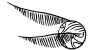
\includegraphics[scale=0.4]{boccino.png}
        \centering
\end{figure}

Cinque ore prima, Harry si stava intrufolando nel suo dormitorio con le vesti alzate sul capo a mo’ di mascheramento, giusto nel caso in cui qualcuno fosse già sveglio e lo vedesse contemporaneamente all’Harry che giaceva nel suo letto. Non voleva essere costretto a spiegare a qualcuno il suo piccolo problema di Duplicazione Spontanea.

Fortunatamente sembrava che tutti stessero dormendo.

E sembrava anche esserci una scatola, avvolta in carta rossa e verde con un fiocco giallo acceso, appoggiata vicino al suo letto. L’immagine perfetta e stereotipata del regalo di Natale, sebbene non fosse Natale.

Harry strisciò dentro il più sommessamente possibile, nel caso qualcuno avesse messo il proprio Quietus sul minimo.

C’era una busta attaccata alla scatola, chiusa da cera chiara e liscia senza sigillo impresso.

Harry aprì cautamente la busta, e prese la lettera al suo interno.

La lettera diceva:

Questo è il Mantello dell’Invisibilità di Ignotus Peverell, tramandato dai suoi discendenti, i Potter. A differenza di mantelli inferiori e incantesimi, ha il potere di tenerti nascosto, non semplicemente invisibile. Tuo padre me lo prestò per studiarlo poco prima che morisse, e confesso che ne ho fatto molto buon uso negli anni.

In futuro dovrò accontentarmi della Disillusione, temo. È tempo che il Mantello torni a te, suo erede. Avevo pensato di fartene dono a Natale, ma desiderava tornare in mano tua prima di allora. Sembra che si aspetti che tu ne abbia bisogno. Usalo bene.

Senza dubbio stai già pensando a ogni sorta di meraviglioso scherzo, come quelli che tuo padre praticò ai suoi tempi. Se ogni sua malefatta fosse nota, tutte le donne in Grifondoro si riunirebbero per profanare la sua tomba. Non cercherò di impedire che la storia si ripeta, ma stai estremamente attento a non farti scoprire. Se Silente intravvedesse la possibilità di possedere uno dei Doni della Morte, non se la farebbe scappare fino all’ultimo dei suoi giorni.

Un Buon Natale di cuore a te.

La nota non era firmata.

\begin{figure}[h!]
        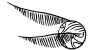
\includegraphics[scale=0.4]{boccino.png}
        \centering
\end{figure}

«Aspettate», disse Harry fermandosi all’improvviso mentre gli altri ragazzi stavano per lasciare il dormitorio Corvonero. «Scusatemi, c’è qualcos’altro che devo fare col mio baule. Vi seguirò a colazione tra un paio di minuti.»

Terry Boot guardò Harry accigliato. «Faresti meglio a non pensare di mettere le mani nella nostra roba.»

Harry alzò una mano. «Giuro che non intendo fare nulla del genere ad alcuna delle tue cose, che intendo solamente accedere a oggetti che io stesso posseggo, che non ho intenzione di giocare scherzi o altre cose discutibili contro nessuno di voi, e che non prevedo che queste intenzioni cambino prima che io scenda nella Sala Grande per colazione.»

Terry aggrottò la fronte. «Aspetta, cosa –»

«Non ti preoccupare», disse Penelope Clearwater, che era lì per guidarli. «Non c’erano scappatoie. Ben formulata, Potter, dovresti fare l’avvocato.»

Harry Potter sbatté le palpebre. Ah, già, un prefetto Corvonero. «Grazie», disse. «Credo.»

«Quando cercherai di raggiungere la Sala Grande, ti perderai.» Penelope lo disse come fosse un fatto semplice e indiscutibile. «Appena ciò avviene, chiedi a un ritratto come raggiungere il primo piano. Rivolgiti a un altro ritratto nell’istante in cui sospetti di esserti perso di nuovo. Specialmente se sembra che tu salga sempre più in alto. Se arrivi più in alto di quanto dovrebbe essere l’intero castello, fermati e aspetta le squadre di soccorso. Altrimenti ti rivedremo tra quattro mesi e sarai più vecchio di cinque mesi e vestito con un perizoma e ricoperto di neve e questo se rimani all’interno del castello.»

«Ricevuto», disse Harry deglutendo con difficoltà. «Uhm, non dovreste dirlo subito a tutti gli studenti?»

Penelope sospirò. «Cosa, tutto quello? Ci vorrebbero settimane. Lo imparerete strada facendo.» Si girò per andarsene, seguita dagli altri studenti. «Se non ti vedo a colazione entro trenta minuti, Potter, darò inizio alle ricerche.»

Quando tutti se ne furono andati, Harry attaccò la nota al suo letto – aveva già scritto quella e tutte le altre note, lavorando nel livello sotterraneo del suo baule prima che tutti si svegliassero. Poi entrò con cautela nel campo del Quietus e tirò via il Mantello dell’Invisibilità dalla forma dormiente di Harry-1.

E solo per un impulso malizioso, Harry mise il Mantello nella borsa di Harry-1, sapendo che perciò era già nel suo.

\begin{figure}[h!]
        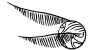
\includegraphics[scale=0.4]{boccino.png}
        \centering
\end{figure}

«Posso provvedere affinché il messaggio sia consegnato a Cornelion Flubberwalt», disse il dipinto di un uomo dall’aria aristocratica e, in effetti, con un naso perfettamente normale. «Ma posso chiedere da dove proviene originariamente?»

Harry alzò le spalle con ingegnosa impotenza. «Mi è stato detto che è stato pronunciato da una voce cavernosa che è risuonata da un vuoto nell’aria stessa, un vuoto che si era aperto su di un feroce abisso.»

\begin{figure}[h!]
        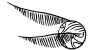
\includegraphics[scale=0.4]{boccino.png}
        \centering
\end{figure}

«Ehi!» disse Hermione in tono indignato dal suo posto dall’altro lato del tavolo della colazione. «Quello è il dolce di tutti! Non puoi prendere un’intera torta e mettertela nella borsa!»

«Non sto prendendo una torta, ne sto prendendo due. Scusatemi tutti, devo andare!» Harry ignorò le grida di sdegno e lasciò la Sala Grande. Aveva bisogno di arrivare alla classe di Erbologia un po’ in anticipo.

\begin{figure}[h!]
        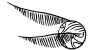
\includegraphics[scale=0.4]{boccino.png}
        \centering
\end{figure}

La professoressa Sprout lo guardò acutamente. «E come fai lei a sapere cosa stanno pensando di fare i Serpeverde?»

«Non posso rivelare la mia fonte», disse Harry. «Anzi, devo chiederle di far finta che questa conversazione non sia mai avvenuta. Faccia come se fosse casualmente incappata in loro mentre era in giro per una faccenda o qualcosa del genere. Correrò avanti appena Erbologia termina. Penso di poter distrarre i Serpeverde mentre lei arriva. Non è facile spaventarmi o intimidirmi, e non penso che oseranno ferire seriamente il Ragazzo-Che-È-Sopravvissuto. Anche se… non le sto chiedendo di correre per i corridoi, ma apprezzerei se non si attardasse lungo la strada.»

La professoressa Sprout lo guardò per un lungo istante, poi la sua espressione si addolcì. «Faccia attenzione, Harry Potter. E… grazie.»

«Abbia solo cura di non arrivare tardi», disse Harry. «E ricordi, quando arriverà, lei non si aspetterà di vedermi e questa conversazione non è mai avvenuta.»

\begin{figure}[h!]
        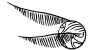
\includegraphics[scale=0.4]{boccino.png}
        \centering
\end{figure}

Fu orribile, vedersi strattonare Neville fuori dal circolo dei Serpeverde. Neville aveva avuto ragione, aveva usato troppa forza, assolutamente troppa forza.

«Ciao», disse Harry gelidamente. «Io sono il Ragazzo-Che-È-Sopravvissuto.»

Otto ragazzi del primo anno, per lo più della stessa altezza. Uno di loro aveva una cicatrice sulla fronte e non si stava comportando come gli altri.

Oh volesse un potere darci il piccolo dono

Di veder noi stessi come gli altri ci vedono!

Ci libererebbe da molti abbagli,

E stupide credenze –

La professoressa McGonagall aveva ragione. Il Cappello Smistatore aveva ragione. Era chiaro una volta che lo vedevi dall’esterno.

C’era qualcosa di sbagliato in Harry Potter.




% !TeX root = Harry.tex

\chapter{Coscienziosità}
\label{capitolo:15}

\emph{«Sono certo che troverò il tempo da qualche parte.»}

~\\
~\\

«\textit{Frigideiro!}»

Harry mise un dito nel bicchiere d’acqua appoggiato sul banco. Avrebbe dovuto essere fredda. Ma tiepida era inizialmente, e tiepida era rimasta. Ancora una volta.

Harry si sentiva veramente, veramente preso in giro.

C’erano centinaia di romanzi fantasy sparsi per casa Verres. Harry ne aveva letti un bel po’. E iniziava a essere evidente che avesse un misterioso lato oscuro. Così, dopo che il bicchiere d’acqua si era rifiutato di cooperare le prime volte, Harry aveva gettato uno sguardo in giro per l’aula di Incantesimi per assicurarsi che nessuno lo stesse osservando, e poi aveva fatto un respiro profondo, si era concentrato, e aveva fatto in modo di infuriarsi. Aveva pensato ai Serpeverde che perseguitavano Neville, e al gioco in cui qualcuno gettava a terra i tuoi libri ogni volta che tentavi di prenderli di nuovo. Aveva pensato a quello che Draco Malfoy aveva detto circa la decenne ragazza Lovegood e di come funzionava davvero il Wizengamot…

E la furia era entrata nel suo sangue, aveva tenuto la bacchetta in una mano che tremava per l’odio e aveva detto in un tono gelido «Frigideiro!» e non era successo assolutamente niente.

Harry era stato \textit{truffato}. Voleva scrivere a qualcuno e chiedere un \textit{rimborso} per il suo lato oscuro, che chiaramente \textit{doveva} avere un irresistibile potere magico, ma che si era rivelato essere \textit{difettoso}.

«\textit{Frigideiro!}» disse di nuovo Hermione dal banco accanto a lui. La sua acqua era ghiaccio solido e c’erano cristalli bianchi che si stavano formando sul bordo del bicchiere. Sembrava essere totalmente concentrata sul proprio lavoro e niente affatto consapevole che gli altri studenti la fissavano con occhi carichi d’odio, cosa che era (a) una dimostrazione di pericolosa disattenzione da parte sua o (b) un’interpretazione perfetta elevata al livello di arte sopraffina.

«Oh, \textit{molto} bene, signorina Granger!» squittì Filius Flitwick, il loro Professore di Incantesimi e il Preside di Corvonero, piccolo ometto senza segni visibili di essere stato in passato un campione di duelli. «Eccellente! Stupendo!»

Harry si era aspettato di essere, nel peggiore dei casi, secondo alle spalle di Hermione. Harry avrebbe preferito che \textit{lei} fosse la \textit{sua} rivale, naturalmente, ma avrebbe potuto accettare anche il contrario.

Giunti a lunedì, Harry si stava indirizzando verso il fondo della classe, una posizione per cui stava socievolmente rivaleggiando con tutti gli altri studenti educati da Babbani tranne Hermione. Che era tutta sola e senza rivali in testa, poverina.

Il professor Flitwick stava in piedi sopra il banco di una degli altri Nati babbani e stava sommessamente correggendo il modo in cui impugnava la bacchetta.

Harry guardò Hermione. Deglutì. Nello schema delle cose, era il ruolo scontato per lei… «Hermione?» Harry disse timidamente. «Hai una vaga idea di quello che potrei fare di sbagliato?»

Gli occhi di Hermione si illuminarono di una terribile luce di disponibilità e qualcosa nei recessi del cervello di Harry urlò per la disperata umiliazione.

Cinque minuti più tardi, l’acqua di Harry sembrava notevolmente più fredda rispetto alla temperatura ambiente ed Hermione gli aveva dato un paio di pacche sulle spalle verbali e detto di pronunciare con più attenzione la volta successiva, e se n’era andata per aiutare qualcun altro.

Il professor Flitwick le aveva concesso un punto per averlo aiutato.

Harry stava stringendo i denti così forte che la mascella gli faceva male e questo non stava aiutando la sua pronuncia.

\textit{Non mi importa se si tratta di concorrenza sleale. So esattamente quello che farò con due ore in più ogni giorno. Andrò a sedermi nel mio baule e studierò fino a quando sarò alla pari con Hermione Granger.}

\begin{figure}[h!]
        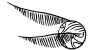
\includegraphics[scale=0.4]{boccino.png}
        \centering
\end{figure}

«La Trasfigurazione è una delle magie più complesse e pericolose che imparerete a Hogwarts», disse la professoressa McGonagall. Non c’era alcuna traccia di levità sul volto della vecchia strega austera. «Chiunque combini pasticci nel mio corso se ne andrà per non tornare più. Siete stati avvertiti.»

La sua bacchetta scese a battere sulla cattedra, che dolcemente si rimodellò in un maiale. Un paio di studenti Nati babbani emisero piccoli guaiti. Il maiale si guardò intorno e sbuffò, sembrava confuso, e poi divenne nuovamente una cattedra.

La Professoressa di Trasfigurazione guardò la classe intorno a sé, e poi i suoi occhi si posarono su di uno studente.

«Signor Potter», disse la professoressa McGonagall. «Ha ricevuto i libri di scuola soltanto un paio di giorni fa. Ha già iniziato a leggere il suo libro di testo di Trasfigurazione?»

«No, mi dispiace professoressa», disse Harry.

«Non c’è bisogno di chiedere scusa, signor Potter, se foste stati tenuti a leggerlo in anticipo vi sarebbe stato detto di farlo.» McGonagall batté le dita sulla cattedra di fronte a lei. «Signor Potter, le andrebbe di indovinare se questa è una cattedra che ho trasfigurato in un maiale, o se inizialmente era un maiale e ho brevemente rimosso la Trasfigurazione? Se avesse letto il primo capitolo del libro di testo, lo saprebbe.»

Harry aggrottò leggermente la fronte. «Direi che sarebbe più semplice iniziare con un maiale, in quanto se si partisse da una cattedra, potrebbe non sapere come stare in piedi.»

La professoressa McGonagall scosse la testa. «Non glie ne faccio una colpa, signor Potter, ma la risposta corretta è che a Trasfigurazione \textit{non} ci interessa tirare a indovinare. Le risposte sbagliate saranno valutate con estrema severità, le domande lasciate in bianco saranno valutate con grande indulgenza. Dovete imparare a riconoscere ciò che non conoscete. Se vi pongo una qualunque domanda, non importa quanto ovvia o elementare, e rispondete ‘Non ne sono sicuro’, non la valuterò a vostro sfavore e chiunque rida perderà punti per la sua Casa. Sa dirmi perché esiste questa regola, signor Potter?»

\textit{Poiché un singolo errore a Trasfigurazione può essere incredibilmente pericoloso.} «No.»

«Corretto. Trasfigurazione è più pericolosa di Apparizione, che non viene insegnata prima del sesto anno. Purtroppo, Trasfigurazione deve essere appresa e praticata in giovane età per massimizzare la vostra capacità da adulti. Quindi è una materia pericolosa, e dovreste essere alquanto spaventati dall’idea di commettere degli errori, perché nessuno dei miei studenti si è mai fatto male seriamente e io sarò \textit{estremamente offesa} se foste la prima classe a \textit{rovinare questo mio primato}.»

Diversi studenti deglutirono.

La professoressa McGonagall si alzò e si avvicinò alla parete dietro la cattedra, che reggeva una tavola di legno levigata. «Ci sono molte ragioni per cui Trasfigurazione è pericolosa, ma una ragione domina su tutte le altre.» Tirò fuori una penna d’oca con una spessa estremità, e la usò per disegnare delle lettere in rosso; poi le sottolineò, usando la stessa penna, in blu:

\begin{center}
\underline{\textsc{Trasfigurazione non è permanente!}}
\end{center}

«Trasfigurazione non è permanente!» disse la professoressa McGonagall. «Trasfigurazione non è permanente! Trasfigurazione non è permanente! Signor Potter, supponga che uno studente Trasfigurasse un blocco di legno in una coppa d’acqua, e lei la bevesse. Cosa pensa le accadrebbe quando la Trasfigurazione svanisse?» Ci fu una pausa. «Mi scusi, non avrei dovuto chiederlo a lei, signor Potter, ho dimenticato che ha ricevuto il dono di una fantasia insolitamente pessimista –»

«Non è un problema», disse Harry, deglutendo con difficoltà. «Dunque, la prima risposta è che \textit{non lo so}», la professoressa annuì in approvazione, «ma \textit{immagino} che ci possa essere… del legno nel mio stomaco, e nel mio flusso sanguigno e in tutta quell’acqua che è stata assorbita dai tessuti del mio corpo — che fosse polpa di legno o legno pieno o…» La sua comprensione della magia lo tradì. Non era in grado di capire in che modo il legno si mappasse nell’acqua, tanto per cominciare, quindi non riusciva a comprendere che cosa sarebbe accaduto dopo che le molecole d’acqua fossero state rimescolate in seguito ai normali moti termici e la magia fosse svanita e la mappatura invertita.

Il volto di McGonagall era severo. «Come il signor Potter ha correttamente dedotto, si sarebbe ammalato gravemente e avrebbe avuto bisogno di un immediato trasferimento via Metropolvere al St. Mungo’s Hospital, per avere una minima speranza di sopravvivenza. Per favore, aprite i vostri libri di testo a pagina 5.»

Anche se nessun suono proveniva dalla foto in movimento, si poteva capire che la donna con la pelle orribilmente scolorita stava urlando.

«Il criminale che inizialmente trasfigurò dell’oro in vino e lo diede da bere a questa donna, ‘a saldo del debito’ come disse lui, ricevette una condanna a dieci anni ad Azkaban. Per favore, andate a pagina 6. Questo è un Dissennatore. Sono i guardiani di Azkaban. Vi succhiano via la magia, la vita e qualunque pensiero felice abbiate. La figura a pagina 7 ritrae il criminale dieci anni dopo, al suo rilascio. Noterete che è morto — sì, signor Potter?»

«Professoressa», chiese Harry, «se dovesse accadere il peggio in un caso simile, c’è qualche modo di \textit{sostenere} la Trasfigurazione?»

«No», disse la professoressa McGonagall con voce piatta. «Sostenere una Trasfigurazione è un drenaggio costante della vostra magia che scala con le dimensioni della forma dell’obbiettivo. E avreste bisogno di rimettervi in contatto col bersaglio ogni poche ore, cosa che è, in un caso come questo, impossibile. Disastri come questo sono \textit{irrecuperabili!}»

La professoressa McGonagall si inclinò in avanti, l’espressione sul viso molto severa. «Assolutamente mai, in nessuna circostanza, Trasfigurerete qualunque cosa in un liquido o in un gas. Niente acqua, niente aria. Nulla di simile all’acqua, nulla di simile all’aria. Anche se non va bevuto. I liquidi \textit{evaporano}, piccole parti di essi finiscono nell’aria. Non Trasfigurerete nulla che vada bruciato. Produrrebbe del fumo e qualcuno potrebbe respirare quel fumo! Non Trasfigurerete mai qualunque cosa che in linea di principio possa finire nel corpo di qualcuno in qualunque modo. Niente cibo. Nulla che \textit{sembri} del cibo. Neppure per un divertente scherzetto in cui volete dire alle vittime della vostra torta di fango prima che la mangino realmente. Non lo farete mai. Punto. Dentro questa classe o fuori di essa o \textit{ovunque}. Questo è ben chiaro a \textit{ogni singolo studente?}»

«Sì» dissero Harry, Hermione, e pochi altri. Il resto sembrava essere senza parole.

«\textit{Questo è ben chiaro a ogni singolo studente?}»

«Sì», dissero o mormorarono o sussurrarono.

«Se infrangerete una qualunque di queste regole non studierete più Trasfigurazione durante tutta la vostra permanenza a Hogwarts. Ripetete con me. Non Trasfigurerò mai nulla in un liquido o in un gas.»

«Non Trasfigurerò mai nulla in un liquido o in un gas», dissero gli studenti in un coro irregolare.

«Ancora! Più forte! Non Trasfigurerò mai nulla in un liquido o in un gas.»

«Non Trasfigurerò mai nulla in un liquido o in un gas.»

«Non Trasfigurerò mai nulla che sembri del cibo o qualunque altra cosa che finisce all’interno di un corpo umano.»

«Non Trasfigurerò mai nulla che debba essere bruciato perché potrebbe fare del fumo.»

«Non Trasfigurerete mai nulla che sembri del denaro, incluso il denaro babbano», disse la professoressa McGonagall. «I goblin hanno dei metodi per scoprire chi l’ha fatto. E per quanto riguarda la legge, la nazione goblin è in stato di \textit{guerra} permanente con tutti i falsari magici. Non manderanno degli Auror. Manderanno un esercito.»

«Non Trasfigurerò mai nulla che sembri del denaro», ripeterono gli studenti.

«E \textit{soprattutto}», disse la professoressa McGonagall, «non Trasfigurerete nessun essere vivente, \textit{specialmente voi stessi}. Vi farebbe ammalare gravemente e persino morire, a seconda di come vi Trasfigurereste e per quanto tempo manterreste il cambiamento.» La professoressa McGonagall fece una pausa. «Il signor Potter sta alzando la mano perché ha visto una trasformazione Animagus — precisamente un umano trasformarsi in un gatto e poi riassumere la propria forma. Ma una trasformazione Animagus non è una Trasfigurazione \textit{libera.}»

La professoressa McGonagall prese un piccolo blocchetto di legno dalla tasca. Con un tocco della sua bacchetta divenne una palla di vetro. Poi disse «\textit{Crystferrium!}» e la palla di vetro divenne una sfera d’acciaio. La toccò con la bacchetta per l’ultima volta e la sfera d’acciaio divenne un pezzo di legno ancora una volta. «\textit{Crystferrium} trasforma un soggetto di vetro solido in un bersaglio di acciaio solido di forma simile. Non può fare il contrario, né può trasformare una cattedra in un maiale. La forma più generale di Trasfigurazione — Trasfigurazione libera, che imparerete qui — è in grado di trasformare qualunque soggetto in qualunque bersaglio, per lo meno per quanto riguarda la forma fisica. Per questo motivo, Trasfigurazione libera deve essere eseguita senza parole. Usare degli Incantesimi richiederebbe parole differenti per ciascuna differente trasformazione tra soggetto e bersaglio.»

La professoressa McGonagall indirizzò ai suoi studenti uno sguardo penetrante. «\textit{Alcuni} insegnanti iniziano con gli Incantesimi di Trasfigurazione per poi passare successivamente alla Trasfigurazione libera. Sì, all’inizio questo approccio sarebbe più facile. Ma potrebbe creare una \textit{forma mentis} che più tardi comprometterebbe le vostre capacità. Qui imparerete la Trasfigurazione libera \textit{sin dal principio}, cosa che richiede che lanciate l’incantesimo senza parole, tenendo la forma del soggetto, la forma del bersaglio, e la trasformazione all’interno della vostra mente.»

«E per rispondere alla domanda del signor Potter», continuò la professoressa McGonagall, «è la Trasfigurazione \textit{libera} che non dovete mai lanciare su nessun soggetto vivo. Ci sono Incantesimi e pozioni che possono trasformare con sicurezza e reversibilmente bersagli vivi in modo \textit{limitato}. Un Animagus con un arto mancante continuerà a non avere quell’arto dopo la trasformazione, per esempio. La Trasfigurazione libera \textit{non è} sicura. Il vostro corpo muterà mentre è Trasfigurato — respirare, per esempio, implica una perdita costante della materia del corpo in favore dell’aria circostante. Quando la Trasfigurazione si estingue e il vostro corpo cerca di ritornare alla sua forma \textit{originale}, non sarà più in grado di farlo. Se appoggiate la vostra bacchetta al vostro corpo e immaginate di avere capelli dorati, in seguito i vostri capelli cadranno. Se vi visualizzate come qualcuno con la pelle più chiara, sarete costretti a una lunga permanenza al St. Mungo’s. E se vi Trasfigurerete in un corpo adulto, allora, quando la Trasfigurazione cesserà, voi morirete.»

Questo spiegava perché aveva visto cose come ragazzi grassi, o ragazze meno che perfettamente carine. O persone anziane, se è per questo. Tutto ciò non sarebbe accaduto se fosse stato possibile Trasfigurare sé stessi ogni mattina… Harry alzò la mano e cercò di attirare l’attenzione della professoressa McGonagall con gli occhi.

«\textit{Sì}, signor Potter?»

«È possibile trasfigurare un soggetto vivente in un bersaglio che è statico, come una moneta — no, mi scusi, mi dispiace, diciamo in una semplice sfera di acciaio?»

La professoressa McGonagall scosse la testa. «Signor Potter, anche gli oggetti inanimati subiscono piccoli cambiamenti interni nel corso del tempo. Non ci sarebbero cambiamenti visibili nel vostro corpo, e per il primo minuto non vi accorgereste di nulla. Ma in un’ora vi ammalereste, e in un giorno sareste morti.»

«Ehm, mi scusi, quindi se avessi letto il primo capitolo avrei potuto \textit{immaginare} che la cattedra era in origine una cattedra e non un maiale», disse Harry, «ma solo se avessi fatto l’ipotesi \textit{ulteriore} che non volesse uccidere il maiale, cosa che potrebbe \textit{sembrare} molto probabile, ma –»

«Prevedo che valutare i suoi compiti sarà una fonte inesauribile di gioia per me, signor Potter. Ma se ha altre domande, posso chiederle di attendere fino a dopo la lezione?»

«Nessun’altra domanda, professoressa.»

«Ora ripetete dopo di me», disse la professoressa McGonagall. «Non proverò mai a Trasfigurare nessun soggetto vivo, specialmente me stesso, se non specificatamente istruito a farlo usando un Incantesimo specializzato o una pozione.»

«Se non sono certo che una Trasfigurazione sia sicura, non la proverò finché non l’avrò chiesto alla professoressa McGonagall o al professor Flitwick o al professor Snape o al Preside, che sono le uniche autorità riconosciute per la Trasfigurazione a Hogwarts. Chiedere a un altro studente non è accettabile, anche se affermassero di ricordare di aver fatto la stessa domanda.»

«Anche se l’attuale Professore di Difesa di Hogwarts mi dicesse che una Trasfigurazione è sicura, e anche se vedessi il Professore di Difesa effettuarla senza che nulla di male accada, non la proverò io stesso.»

«Ho il diritto assoluto di rifiutarmi di effettuare ogni Trasfigurazione che mi renda minimamente nervoso. Poiché neppure il Preside di Hogwarts può ordinarmi di fare diversamente, non accetterò certamente un tale ordine dal Professore di Difesa, anche se il Professore di Difesa minacciasse di sottrarre cento punti alla mia Casa e di farmi espellere.»

«Se violerò una qualunque di queste regole non studierò più Trasfigurazione durante la mia permanenza a Hogwarts.»

«Ripeteremo queste regole all’inizio di ogni lezione per il primo mese», disse la professoressa McGonagall. «E ora, iniziamo con dei fiammiferi come soggetti e degli aghi come bersagli… mettete via le vostre bacchette, con ‘iniziamo’ intendevo dire inizierete a prendere appunti.»

Mezz’ora prima della fine della lezione, la professoressa McGonagall distribuì i fiammiferi.

Alla fine della lezione, Hermione aveva un fiammifero argenteo e il resto della classe, Nati babbani o meno, aveva esattamente ciò con cui aveva iniziato.

La professoressa McGonagall le assegnò un altro punto per Corvonero.

\begin{figure}[h!]
        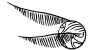
\includegraphics[scale=0.4]{boccino.png}
        \centering
\end{figure}

Dopo che la lezione di Trasfigurazione fu terminata, Hermione andò al banco di Harry, proprio mentre Harry stava rimettendo i libri nella borsa.

«Sai», disse Hermione con un’espressione innocente sul viso, «ho guadagnato due punti per Corvonero oggi.»

«Già», disse laconicamente Harry.

«Ma non è all’altezza dei tuoi \textit{sette} punti», continuò lei. «Credo semplicemente di non essere intelligente come te.»

Harry finì di inserire i propri compiti nella borsa e si girò verso Hermione con gli occhi socchiusi. Si era davvero dimenticato di quello.

Lei gli \textit{sbatté le ciglia}. «Abbiamo lezioni tutti i giorni, però. Mi chiedo quanto tempo ti ci vorrà per trovare qualche altro Tassofrasso da salvare? Oggi è lunedì. Quindi hai fino a giovedì.»

I due si fissarono l’un l’altro negli occhi, senza battere ciglio.

Harry parlò per primo. «Naturalmente capisci che questo significa guerra.»

«Non sapevo che fossimo in pace.»

Tutti gli altri studenti stavano ora guardando con occhi affascinati. Tutti gli altri studenti, oltre, purtroppo, alla professoressa McGonagall.

«Oh, signor Potter», cinguettò la professoressa McGonagall dall’altra parte della stanza, «ho una buona notizia per lei. Madam Pomfrey ha approvato il suo suggerimento per prevenire le rotture nei suoi Cancelletti ruotanti, e l’idea è quella di finire il lavoro entro la fine della prossima settimana. Direi che questo meriti… diciamo dieci punti per Corvonero.»

Hermione rimase a bocca aperta per la sensazione di tradimento e di stupore. Harry immaginò che il proprio volto non apparisse molto diverso.

«\textit{Professoressa…}» sibilò Harry.

«Quei dieci punti sono \textit{indiscutibilmente} meritati, signor Potter. Non assegnerei mai dei punti per un capriccio. Per lei può essere stato semplicemente notare qualcosa di fragile e suggerire un modo per proteggerlo, ma i Cancelletti ruotanti sono costosi, e il Preside \textit{non è stato} contento l’ultima volta che se n’è rotto uno.» La professoressa McGonagall sembrò pensierosa. «Accidenti, mi chiedo se qualche altro studente abbia mai guadagnato diciassette punti nel suo primo giorno di lezioni. Devo controllare, ma sospetto che questo sia un nuovo primato. Forse dovremmo fare un annuncio a cena?»

«\textsc{Professoressa!}» strillò Harry. «Questa è la \textit{nostra} guerra! La smetta di intromettersi!»

«Ora ha fino a giovedì della \textit{prossima} settimana, signor Potter. A meno che, naturalmente, lei non sia coinvolto in qualche genere di guaio e \textit{perda} dei punti prima di allora. Rivolgendosi a un’insegnante in maniera irriguardosa, per esempio.» La professoressa McGonagall appoggiò un dito sulla guancia e sembrò riflettere. «Mi aspetto che lei raggiunga i numeri negativi prima della fine di venerdì.»

La bocca di Harry si chiuse di scatto. Lanciò il suo miglior Sguardo Mortale a McGonagall, ma ella sembrò trovarlo solo divertente.

«Sì, senz’altro un annuncio a pranzo», rifletté la professoressa McGonagall. «Ma non sarebbe utile offendere i Serpeverde, quindi l’annuncio sarà breve. Solo il numero di punti e la faccenda del primato… e se qualcuno dovesse venire da lei per essere aiutato e fosse deluso che non ha neppure iniziato a leggere i suoi libri di testo, potrebbe sempre mandarlo dalla signorina Granger.»

«\textit{Professoressa!}» disse Hermione in un tono acuto.

La professoressa McGonagall la ignorò. «Accipicchia, mi chiedo quanto ci vorrà alla signorina Granger per fare qualcosa che meriti un annuncio a cena? Non vedo l’ora di scoprirlo, qualunque cosa sia.»

Harry ed Hermione, di tacito e comune accordo, si voltarono e si precipitarono fuori dalla classe. Furono seguiti da una scia di Corvonero ipnotizzati.

«Uhm», disse Harry. «Siamo ancora d’accordo per il dopo cena?»

«Naturalmente», disse Hermione. «Non vorrei che rimanessi ancora più indietro nello studio.»

«Certo, grazie. E lasciami dire che per quanto tu sia già brillante, non posso fare a meno di chiedermi come sarai una volta che avrai ricevuto un po’ di formazione di base in razionalità.»

«È davvero così utile? Non sembra averti aiutato in Incantesimi o Trasfigurazione.»

Ci fu una breve pausa.

«Beh, ho ricevuto i mie libri di scuola appena quattro giorni fa. È per questo che ho dovuto guadagnare quei diciassette punti senza usare la mia bacchetta.»

«Quattro giorni fa? Forse non puoi leggere otto libri in quattro giorni, ma avresti potuto leggerne almeno \textit{uno}. Quanti giorni ti ci vorranno per finire con questo ritmo? Sai tutta quella matematica, quindi puoi dirmi quanto fa otto, per quattro, diviso zero?»

«Ho le lezioni ora, che tu non hai avuto, ma i fine settimana sono liberi, quindi… limite di otto per quattro diviso epsilon per epsilon che tende a zero più… 10:47 di domenica.»

«Io l’ho fatto in \textit{tre} giorni, veramente.»

«E 14:47 di sabato sia, allora. Sono certo che troverò il tempo da qualche parte.»

E fu sera e fu mattina, il primo giorno.




% !TeX root = Harry.tex

\chapter{Pensiero laterale}
\label{capitolo:16}

\emph{«Non sono uno psicopatico, sono solo molto creativo.»}

~\\
~\\

Non appena mercoledì entrò nell’aula di Difesa, Harry seppe che \textit{quella} materia sarebbe stata \textit{differente}.

Si trattava, per cominciare, della più grande aula che avesse visto a Hogwarts, analoga all’aula di un’università di prestigio, con livelli sovrapposti di banchi che fronteggiavano un gigantesco palco piatto di marmo bianco. L’aula era situata in alto nel castello — al quinto piano — e Harry sapeva che quella era tutta la spiegazione che avrebbe ricevuto su come un’aula di quelle dimensioni potesse trovarvi posto. Stava diventando chiaro che Hogwarts semplicemente non aveva una geometria, euclidea o altra; aveva connessioni, non direzioni.

A differenza di un’aula universitaria, non c’erano file di sedili pieghevoli; invece c’erano dei banchi di legno e delle sedie di legno, allineati in una curva lungo ciascun livello dell’aula, piuttosto normali per Hogwarts. Tranne che ogni banco aveva un oggetto piatto, bianco, rettangolare e misterioso appoggiato sopra.

Al centro della gigantesca piattaforma, su di una piccola pedana di marmo scuro, c’era la solitaria scrivania dell’insegnante. Alla quale era seduto Quirrell, accasciato sulla sedia, la testa che ciondolava all’indietro, sbavando leggermente sopra le vesti.

\textit{Cosa mi ricorda…?}

Harry era arrivato a quella lezione così presto che nessun altro studente era ancora lì. (Il vocabolario era imperfetto quando si trattava di descrivere il viaggio nel tempo; in particolare, mancava di qualsiasi parola capace di esprimere quanto fosse comodo.) Quirrell non sembrava essere… funzionale… in quel momento, e Harry non aveva particolarmente voglia di avvicinarglisi, comunque.

Scelse un posto, s’inerpicò fino ad esso, si sedette, e recuperò il libro di testo di Difesa. Era arrivato a circa sette ottavi — aveva avuto intenzione di finirlo prima di quella lezione, in realtà, ma stava rimanendo indietro col programma e aveva già usato il Giratempo due volte, quel giorno.

Presto vi furono dei suoni, mentre la classe cominciò a riempirsi. Harry li ignorò.

«Potter? Cosa ci \textit{fai tu} qui?»

\textit{Quella} voce era fuori luogo. Harry alzò lo sguardo. «Draco? Cosa ci fai \textit{tu} in oh mio dio tu hai dei \textit{servitori.}»

Uno dei ragazzi in piedi dietro Draco sembrava avere parecchi muscoli per un undicenne, e l’altro aveva assunto una posa bilanciata piuttosto sospetta.

Il ragazzo dai capelli biondo-bianchi sorrise con un certo compiacimento e fece un cenno dietro di sé. «Potter, ti presento il signor Crabbe», la sua mano si mosse da Muscolo a Bilanciato, «il signor Goyle. Vincent, Gregory, questo è Harry Potter.»

Il signor Goyle inclinò la testa e rivolse a Harry uno sguardo che doveva significare qualcosa ma che finì per sembrare semplicemente strabico. Il signor Crabbe disse «Piacere di conoscerti» in un tono che suonò come se stesse cercando di rendere la sua voce più grave possibile.

Una fugace espressione di sgomento attraversò il viso di Draco, ma fu rapidamente sostituita dal suo ghigno di superiorità.

«Tu hai dei \textit{servitori!}» Harry ripeté. «Dove posso ottenere dei servitori anche \textit{io?}»

Il ghigno di Draco si allargò. «Ho paura, Potter, che il primo passo sia quello di essere Smistati in Serpeverde –»

«Cosa? Non è giusto!»

«– e poi che le vostre famiglie abbiano stretto un accordo da ben prima che nasceste.»

Harry guardò il signor Crabbe e il signor Goyle. Entrambi stavano tentando disperatamente di sembrare minacciosi. Ovvero, piegandosi in avanti, curvando le spalle, tirando fuori il collo e fissandolo.

«Uhm… aspetta», disse Harry. «Tutto questo è stato organizzato \textit{anni} fa?»

«Esattamente, Potter. Mi dispiace ma sei stato sfortunato.»

Il signor Goyle tirò fuori uno stuzzicadenti e iniziò a pulirsi i denti, ancora minaccioso.

«E», disse Harry, «Lucius ha insistito che \textit{non dovevi} crescere conoscendo le tue guardie del corpo, e che dovevi incontrarle solo il tuo primo giorno di scuola.»

Questo cancellò il ghigno dal volto di Draco. «Sì, Potter, sappiamo tutti che sei brillante, tutta la scuola lo sa, ormai puoi smetterla di metterti in mostra –»

«Quindi gli è stato detto per \textit{tutta la loro vita} che sarebbero stati i tuoi servitori e hanno speso \textit{anni} immaginando come dovrebbero essere dei servitori –»

Draco fece una smorfia.

«– e cosa peggiore, \textit{loro} si \textit{conoscono} e \textit{hanno fatto pratica} –»

«Il capo t’ha detto che ti devi stare muto», brontolò il signor Crabbe. Il signor Goyle addentò lo stuzzicadenti, tenendolo in bocca, e usò una mano per scrocchiare le nocche dell’altra.

«\textit{Vi ho detto di non fare così davanti a Harry Potter!}»

I due sembrarono un po’ imbarazzati e il signor Goyle si mise rapidamente lo stuzzicadenti in una tasca posteriore della veste.

Ma nel momento in cui Draco diede loro le spalle per rivolgersi di nuovo a Harry, tornarono a farsi minacciosi.

«Ti chiedo scusa», disse Draco rigidamente, «per l’insulto che questi \textit{imbecilli} ti hanno recato.»

Harry diede un’occhiata significativa al signor Crabbe e al signor Goyle. «Direi che sei un po’ duro con loro, Draco. \textit{Io} penso si comportino esattamente come vorrei che i \textit{miei} servitori agissero. Voglio dire, se avessi qualche servitore.»

Draco rimase a bocca aperta.

«Oh, Gregory, ma che questo sta provando a portarci via dal capo nostro, eh?»

«Sono sicuro che il signor Potter non sarebbe così stupido.»

«Oh, non me lo sognerei neppure», disse Harry tranquillamente. «È solo una cosa da tenere a mente se il vostro datore di lavoro attuale sembrasse ingrato. Inoltre, non fa mai male avere altre offerte, mentre si stanno negoziando le proprie condizioni di lavoro, giusto?»

«Che ci sta a fare \textit{questo} a Corvonero?»

«Non me lo immagino, signor Crabbe.»

«\textit{Smettetela}, entrambi», disse Draco a denti stretti. «Questo è un \textit{ordine}.» Con uno sforzo visibile, trasferì l’attenzione nuovamente su Harry. «Ad ogni modo, che ci fai alla lezione di Difesa dei Serpeverde?»

Harry aggrottò la fronte. «Aspetta.» La sua mano andò alla borsa. «Orario.» Guardò sulla pergamena. «Difesa, 14:30, e ora sono le…» Harry guardò il proprio orologio meccanico, che faceva le 11:23. «14:23, a meno che non abbia perso traccia del tempo. È così?» Se sì, bene, Harry sapeva come raggiungere qualunque lezione si \textit{supponeva} dovesse seguire in quel momento. Cielo, amava il suo Giratempo e un giorno, quando fosse stato abbastanza grande, si sarebbero sposati.

«No, sembra giusto», disse Draco, apparentemente confuso. Il suo sguardo si girò per guardare al resto dell’auditorium, che si stava riempiendo di vesti bordate di verde e…

«\textit{Grifondeficienti!}» sputò Draco. «Cosa ci fanno \textit{loro} qui?»

«Hm», fece Harry. «In effetti il professor Quirrell ha detto… ho dimenticato le sue parole esatte… che avrebbe ignorato alcune delle convenzioni didattiche di Hogwarts. Forse ha solo combinato tutti i corsi.»

«Huh», fece Draco. «Sei il primo Corvonero qui dentro.»

«Già. Sono arrivato presto.»

«Che ci fai all’ultima fila, allora?»

Harry batté le palpebre. «Non so, sembrava un buon posto dove sedersi?»

Draco emise un suono beffardo. «Non avresti potuto sederti più lontano dall’insegnante se ci avessi provato.» Il ragazzo dai capelli biondi si fece un po’ più vicino. «Comunque, è vero quello che hai detto a Derrick e alla sua cricca?»

«Chi è Derrick?»

«L’hai colpito con una torta.»

«Due torte, in verità. Cosa gli avrei detto?»

«Che non stava facendo nulla di scaltro o ambizioso e che era una vergogna per Salazar Serpeverde.» Draco stava fissando Harry intensamente.

«Questo… mi suona abbastanza corretto», disse Harry. «Penso fosse qualcosa di più simile a ‘è questa una specie di piano incredibilmente intelligente che ti garantirà un vantaggio futuro o è davvero una disgrazia per la memoria di Salazar Serpeverde come sembra’ o qualcosa del genere. Non ricordo le parole esatte.»

«Stai confondendo tutti, sai», disse il ragazzo dai capelli biondi.

«Eh?» fece Harry onestamente confuso.

«Warrington ha detto che passare molto tempo sotto il Cappello Smistatore è uno dei segni premonitori di un grande Signore Oscuro. Ne parlano tutti, chiedendosi se debbano iniziare a leccarti i piedi giusto nell’evenienza. Poi te ne sei uscito col proteggere un gruppo di \textit{Tassofrasso}, per l’amor di Merlino. \textit{Poi} hai detto a Derrick che è una disgrazia per la memoria di Salazar Serpeverde! Cosa \textit{dovrebbero} pensare tutti?»

«Che il Cappello Smistatore ha deciso di mettermi nella Casa ‘Serpeverde! Sto scherzando! Corvonero!’ e che mi sto comportando di conseguenza.»

Sia il signor Crabbe sia il signor Goyle ridacchiarono, obbligando il signor Goyle a mettersi rapidamente una mano sulla bocca.

«Faremmo meglio a raggiungere i nostri posti», disse Draco. Esitò, si raddrizzò leggermente, parlò un po’ più formalmente. «Ma intendo sinceramente dare seguito alla nostra ultima conversazione e accolgo le tue condizioni.»

Harry annuì. «Ti dispiacerebbe terribilmente se attendessi fino a sabato pomeriggio? Al momento sono coinvolto in una piccola competizione.»

«Una competizione?»

«Vedere se sono in grado di leggere tutti i miei libri di testo tanto velocemente quanto Hermione Granger.»

«Granger», fece eco Draco. I suoi occhi si socchiusero. «La sanguemarcio che pensa di essere Merlino? Se stai cercando di mettere in imbarazzo \textit{lei} allora tutti i Serpeverde ti augurano la \textit{miglior} fortuna, Potter, e io non ti disturberò fino a sabato.» Draco inclinò la testa rispettosamente, e si allontanò, tallonato dai suoi servitori.

\textit{Oh, sarà molto divertente destreggiarsi tra tutto ciò, già lo sento.}

L’aula si stava riempiendo rapidamente di tutti e quattro i colori delle rifiniture: verde, rosso, giallo e blu. Draco e i suoi due amici sembravano impegnati a cercare di ottenere tre posti contigui in prima fila — già occupati, ovviamente. Il signor Crabbe e il signor Goyle si erano fatti vigorosamente minacciosi, ma non sembrò che facesse molto effetto.

Harry si chinò sul suo libro di testo di Difesa e continuò a leggere.

\begin{figure}[h!]
        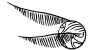
\includegraphics[scale=0.4]{boccino.png}
        \centering
\end{figure}

Alle 14:35, quando la maggior parte dei posti era occupata e nessun altro sembrava stesse arrivando, il professor Quirrell sobbalzò improvvisamente nella sua sedia e si sedette dritto, e il suo volto apparve su tutti gli oggetti bianchi piatti e rettangolari appoggiati sui banchi degli studenti.

Harry fu colto di sorpresa, sia dall’improvvisa apparizione del volto del professor Quirrell sia dalla somiglianza con la televisione babbana. C’era qualcosa di nostalgico e di triste in quello, sembrava tanto un pezzo di casa eppure non lo era veramente…

«Buon pomeriggio, miei giovani apprendisti», disse il professor Quirrell. La sua voce sembrava provenire dallo schermo sul banco e parlare direttamente a Harry. «Benvenuti alla vostra prima lezione di Magia da Battaglia, come avrebbero detto i fondatori di Hogwarts; oppure, come si dà il caso sia chiamata alla fine del ventesimo secolo, di Difesa contro le Arti Oscure.»

Ci fu un raspare frenetico mentre gli studenti, colti di sorpresa, cercarono le loro pergamene o i quaderni di appunti.

«No», disse il professor Quirrell. «Non perdete tempo a scrivere come questa materia era chiamata in passato. Nessuna domanda inutile come questa varrà per i vostri voti in nessuna delle mie lezioni. Questa è una promessa.»

Sentendo ciò, molti studenti si raddrizzarono, sembrando piuttosto scioccati.

Il professor Quirrell sorrideva blandamente. «Quelli di voi che hanno sprecato tempo leggendo i vostri inutili libri di testo di Difesa del primo anno –»

Qualcuno emise un suono soffocato. Harry si chiese se fosse Hermione.

«– potrebbero aver avuto l’impressione che, anche se questo corso è chiamato Difesa Contro le Arti Oscure, in realtà riguardi la difesa dalle Farfalle Incubo, che causano sogni moderatamente brutti, o dalle Lumache Acide, che possono dissolvere completamente una trave di legno di due pollici, se lasciate agire per quasi una giornata.»

Il professor Quirrell si alzò, spingendo indietro la sedia dalla scrivania. Lo schermo sul banco di Harry seguiva ogni sua mossa. Il professor Quirrell avanzò a grandi passi verso la parte anteriore della classe, e urlò:

«L’Ungaro Spinato è più alto di una dozzina di uomini! Sputa fuoco così rapidamente e in modo così preciso da poter sciogliere un Boccino in volo! Una sola Maledizione Mortale lo abbatterà!»

Vi furono sussulti da parte degli studenti.

«Il Troll di montagna è più pericoloso dell’Ungaro Spinato! È sufficientemente forte da masticare l’acciaio! La sua pelle è sufficientemente resistente da sopportare le Maledizioni Stordenti e gli Incantesimi di Taglio! Il suo olfatto è così acuto che può dire da lontano se la sua preda è parte di un branco, o sola e vulnerabile! Cosa più temibile di tutte, il Troll è l’unica tra le creature magiche che sostiene continuamente una sorta di Trasfigurazione su sé stessa — si sta sempre trasformando nel proprio corpo. Se riuscite in qualche modo a strappare il suo braccio ne farà crescere un altro in pochi secondi! Fuoco e acido producono un tessuto cicatriziale che può confondere temporaneamente i poteri rigenerativi di un Troll – per un’ora o due! Sono abbastanza intelligenti da usare i bastoni come strumenti! Il Troll di montagna è la terza macchina per uccidere più perfetta di tutta la Natura! Una sola Maledizione Mortale lo abbatterà.»

Gli studenti sembravano molto sconvolti.

Il professor Quirrell sorrideva piuttosto cupamente. «La vostra triste imitazione di un libro di Difesa del terzo anno vi suggerirà di esporre il Troll di montagna alla luce del sole, che lo bloccherà sul posto. Questo, miei giovani apprendisti, è il tipo di conoscenza inutile che non troverete mai nelle mie lezioni. Non si incontrano Troll di montagna in pieno giorno! L’idea di utilizzare la luce solare per fermarli è dovuta a sciocchi autori di libri di testo che cercano di far mostra della loro padronanza delle minuzie a scapito della praticità. Solo perché c’è un modo ridicolmente oscuro di affrontare i Troll di montagna non significa che dovreste effettivamente provare a usarlo! La Maledizione Mortale non è bloccabile, è inarrestabile e funziona ogni singola volta su qualsiasi cosa abbia un cervello. Se, da maghi adulti, vi trovaste impossibilitati a usare la Maledizione Mortale, allora potrete semplicemente Materializzarvi via! Stessa cosa se foste di fronte alla seconda macchina per uccidere più perfetta, un Dissennatore. Basta che vi Materializziate via!»

«A meno che, naturalmente», disse il professor Quirrell, la sua voce ora più bassa e più dura, «non siate sotto l’influenza di una fattura anti-Materializzazione. No, c’è esattamente un solo mostro che può minacciarvi una volta che siate diventati adulti. Il singolo mostro più pericoloso di tutto il mondo, così pericoloso che nient’altro gli è paragonabile. Il Mago Oscuro. Questa è l’unica cosa che sarà ancora in grado di minacciarvi.»

Le labbra del professor Quirrell erano fissate in una linea sottile. «Vi insegnerò a malincuore abbastanza banalità per ottenere un voto sufficiente ai vostri esami del primo anno sulle parti imposte dal Ministero. Dal momento che l’esatto voto su queste sezioni non farà alcuna differenza per la vostra vita futura, chiunque voglia un voto superiore alla sufficienza è invitato a sprecare il proprio tempo studiando la nostra patetica imitazione di un libro di testo. Il titolo di questo corso non è Difesa Contro i Flagelli Minori. Voi siete qui per imparare a difendervi contro le Arti Oscure. Il che significa, vediamo di essere molto chiari su questo, difendervi dai Maghi Oscuri. Persone dotate di bacchette che vogliono farvi del male e che probabilmente ci riusciranno, a meno che non facciate male loro per primi! Non c’è difesa senza attacco! Non c’è difesa senza combattimento! Questa realtà è ritenuta troppo dura per degli undicenni dai grassi e strapagati politici protetti da Auror che hanno imposto il vostro curriculum. All’abisso quegli sciocchi! Voi siete qui per la materia che è stata insegnata a Hogwarts per ottocento anni! Benvenuti al vostro primo anno di Magia da Battaglia!»

Harry iniziò ad applaudire. Non poteva farne a meno, era stato troppo stimolante.

Una volta che Harry ebbe iniziato ad applaudire ci fu qualche reazione sparpagliata da Grifondoro, e di più da Serpeverde, ma la maggior parte degli studenti sembravano semplicemente troppo sbalorditi per reagire.

Il professor Quirrell fece il gesto di troncare, e l’applauso morì istantaneamente. «Molte grazie», disse il professor Quirrell. «Ora gli avvisi pratici. Ho combinato tutti i miei corsi di Magia da Battaglia del primo anno in uno solo, cosa che mi permette di offrirvi il doppio del tempo in classe rispetto alle Sessioni doppie –»

Si udirono dei rantoli di orrore.

«– un aumento del carico per il quale vi compenserò non assegnandovi alcun compito a casa.»

I rantoli di orrore si interruppero bruscamente.

«Sì, mi avete sentito bene. Vi insegnerò a combattere, non a scrivere una relazione di dodici pollici sul combattimento per lunedì.»

Harry desiderò disperatamente di essere seduto accanto a Hermione in modo da poter vedere l’espressione del suo viso in quel momento, ma d’altra parte era abbastanza sicuro di immaginarsela con precisione.

E poi, Harry era innamorato. Sarebbe stato un matrimonio a tre: Harry, il Giratempo, e il professor Quirrell.

«Per quelli di voi che lo desiderassero, ho organizzato alcune attività di doposcuola che penso troverete molto interessanti ed educative. Volete mostrare al mondo le \textit{vostre} capacità invece di guardare quattordici altre persone giocare a Quidditch? Più di sette persone possono combattere in un esercito.»

Santo \textit{cielo}.

«Queste e altre attività di doposcuola vi permetteranno di guadagnare punti-Quirrell. Cosa sono i punti-Quirrell, vi chiederete? Il sistema dei punti-Casa non soddisfa le mie esigenze, perché rende i punti-Casa troppo rari. Preferisco che i miei studenti sappiano come stanno andando più frequentemente di così. E nelle rare occasioni in cui vi offrirò una prova scritta, si correggerà da sola man mano che la compilerete, e se sbaglierete troppe domande in relazione tra loro, il test vi mostrerà i nomi degli studenti che hanno risposto correttamente a quelle domande, e questi studenti saranno in grado di guadagnare punti-Quirrell aiutandovi.»

… uau. Perché gli altri professori non usavano un sistema simile?

«A che servono i punti-Quirrell, vi chiederete? Per cominciare, dieci punti-Quirrell varranno un punto-Casa. Ma vi permetteranno di guadagnare anche altre agevolazioni. Volete fare il vostro esame a un’ora inusuale? C’è una sessione particolare che preferireste davvero saltare? Scoprirete che posso essere molto flessibile per favorire gli studenti che hanno accumulato abbastanza punti-Quirrell. I punti-Quirrell determineranno il rango di generale degli eserciti. E per Natale — appena prima delle vacanze natalizie — accorderò a qualcuno un desiderio. Ogni impresa relativa alla scuola che rientri nei limiti del mio potere, della mia influenza o, sopratutto, della mia ingegnosità. Sì, ero in Serpeverde e mi sto offrendo per formulare un piano astuto a vostro nome, se questo è quello che ci vuole per raggiungere i vostri desideri. Questo desiderio andrà a chiunque abbia guadagnato più punti-Quirrell in tutti i sette anni.»

Quello sarebbe stato Harry.

«Ora lasciate i vostri libri e oggetti sui vostri banchi — saranno al sicuro, gli schermi veglieranno su di loro per voi — e scendete su questa piattaforma. È il momento di giocare a un gioco chiamato ‘Chi è lo studente più pericoloso della classe’.»

\begin{figure}[h!]
        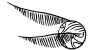
\includegraphics[scale=0.4]{boccino.png}
        \centering
\end{figure}

Harry girò la sua bacchetta nella mano destra e disse «\textit{Ma-ha-su!}»

Ci fu un altro «bing» acuto proveniente dalla sfera blu fluttuante assegnata a Harry dal professor Quirrell come bersaglio. Quel particolare suono indicava un colpo perfetto, che Harry aveva ottenuto in nove dei suoi ultimi dieci tentativi.

Da qualche parte il professor Quirrell aveva scovato un incantesimo che era incredibilmente facile da pronunciare, \textit{e} aveva un movimento della bacchetta ridicolmente semplice, \textit{e} aveva la tendenza a colpire ovunque tu stessi guardando in quel momento. Il professor Quirrell aveva sdegnosamente proclamato che la vera magia da battaglia era molto più difficile. Che quella fattura era del tutto inutile in un combattimento reale. Che si trattava solo di una scarica di magia a malapena organizzata la cui unica difficoltà reale era il puntamento, e che avrebbe prodotto, quando avesse colpito, un dolore equivalente a un pugno forte sul naso. Che l’unico scopo di questa prova era vedere chi fosse rapido a imparare, dal momento che il professor Quirrell era certo che nessuno avesse incontrato precedentemente quella fattura o qualcosa di simile.

A Harry non importava niente di tutto quello.

«\textit{Ma-ha-su!}»

Un \textit{fulmine rosso di energia} fu scagliato dalla sua bacchetta e colpì il bersaglio, e la sfera blu produsse ancora una volta il bing che significava che l’incantesimo \textit{gli era effettivamente riuscito.}

Per la prima volta da quando era arrivato a Hogwarts, Harry si stava sentendo un vero mago. Avrebbe voluto che il bersaglio schivasse come le piccole sfere che Ben Kenobi aveva usato per l’addestramento di Luke, ma per qualche ragione il professor Quirrell aveva invece schierato tutti gli studenti e i bersagli in file ordinate, cosa che garantiva che non si sarebbero colpiti a vicenda.

Così Harry abbassò la bacchetta, balzò sulla destra, alzò di scatto la bacchetta e la rigirò gridando «\textit{Ma-ha-su!}»

Ci fu un «dong» dal trono grave, che significava che l’aveva colpita quasi in pieno.

Harry si mise la bacchetta in tasca, balzò di nuovo a sinistra, estrasse e scagliò un altro fulmine rosso di energia.

L’acuto bing che ne risultò fu facilmente uno dei suoni più soddisfacenti che avesse mai sentito in vita sua. Harry avrebbe voluto urlare trionfante a squarciagola. \textsl{\textsc{Posso fare magie! Temetemi, leggi della fisica, vengo a violarvi!}}

«\textit{Ma-ha-su!}» La voce di Harry era alta, ma appena percettibile sopra la cantilena costante delle grida simili provenienti da tutta la piattaforma.

«Basta», disse la voce amplificata del professor Quirrell. (Non sembrava alta. Aveva un volume normale, e aveva origine appena dietro la tua spalla sinistra, non importa dove fossi disposto rispetto al professor Quirrell.) «Vedo che tutti voi ci siete riusciti almeno una volta, ora.» Le sfere-bersaglio virarono sul rosso e iniziarono a salire verso il soffitto.

Il professor Quirrell era in piedi sulla pedana rialzata al centro della piattaforma, e si appoggiava appena alla sua cattedra con una mano.

«Vi ho detto», disse il professor Quirrell, «che avremmo fatto un gioco chiamato ‘Chi è lo studente più pericoloso della classe’. C’è uno studente in questa classe che ha padroneggiato la Fattura d’Attacco Semplice Sumera più rapidamente di ogni altro –»

Oh blah blah blah.

«– e poi è andato ad aiutare altri sette studenti. Ragion per cui ha guadagnato i primi sette punti-Quirrell assegnati al vostro anno. Venga avanti, Hermione Granger. È il momento della fase successiva del gioco.»

Hermione Granger iniziò a farsi avanti a grandi passi, uno sguardo misto di trionfo e di apprensione sul suo volto. I Corvonero osservavano con orgoglio, i Serpeverde con gelida intensità, e Harry con un chiaro fastidio. Harry aveva fatto bene questa volta. Probabilmente era anche nella metà superiore della classe, ora che tutti avevano dovuto affrontare una magia ugualmente sconosciuta e che Harry aveva letto tutto \textit{Teoria della Magia} di Adalbert Waffling. Eppure \textit{Hermione stava ancora facendo meglio.}

Da qualche parte nei recessi della sua mente c’era la paura che Hermione fosse semplicemente più intelligente di lui.

Ma per ora Harry aveva intenzione di basare le sue speranze sui fatti noti che (a) Hermione aveva letto molto più che i normali libri di testo e (b) Adalbert Waffling era un idiota privo di ispirazione che aveva scritto \textit{Teoria della Magia} per assecondare una commissione scolastica che non aveva una grande opinione degli undicenni.

Hermione raggiunse la pedana centrale e vi salì sopra.

«Hermione Granger ha padroneggiato un incantesimo sconosciuto in appena due minuti, quasi un minuto intero più velocemente del secondo più bravo.» Il professor Quirrell si girò intorno lentamente per osservare tutti gli studenti che lo stavano fissando. «È in grado l’intelligenza della signorina Granger di renderla lo studente più pericoloso della classe? Allora? Che ne pensate?»

Nessuno parve pensare nulla in quel momento. Anche Harry non era sicuro di cosa dovesse dire.

«Allora scopriamolo, no?» disse il professor Quirrell. Si voltò verso Hermione, e fece un gesto a indicando genericamente la classe. «Scelga uno studente a piacere e gli lanci contro la Fattura d’Attacco Semplice Sumera.»

Hermione rimase paralizzata sul posto.

«Forza», disse il professor Quirrell con tranquillità. «Ha lanciato questo incantesimo in maniera perfetta per oltre cinquanta volte. Non causa danni permanenti né è così doloroso. Fa male quanto un pugno forte e dura appena pochi secondi.» La voce del professor Quirrell si fece più dura. «Questo è un ordine diretto del suo professore, signorina Granger. Scelga un bersaglio e lanci la Fattura d’Attacco Semplice.»

Il volto di Hermione era distorto dall’orrore e la bacchetta stava tremando nella sua mano. Le dita di Harry stavano stringendo con forza la sua bacchetta per simpatia. Anche se poteva capire ciò che il professor Quirrell stava cercando di fare. Anche se poteva capire cosa il professor Quirrell stava cercando di dimostrare.

«Se non \textit{solleva} la sua bacchetta per fare fuoco, signorina Granger, perderà un punto-Quirrell.»

Harry fissò Hermione, volendo che guardasse nella sua direzione. La sua mano destra stava battendo con leggerezza sul suo petto. \textit{Scegli me, non ho paura…}

La bacchetta di Hermione si contrasse nella sua mano; poi il suo volto si rilassò ed ella abbassò la bacchetta lungo il fianco.

«No», disse Hermione Granger.

La sua voce era calma, e anche se non era alta, ognuno poté udirla nel silenzio.

«Allora devo toglierle un punto», disse il professor Quirrell. «Questa era una prova, e lei l’ha fallita.»

Ne fu sconvolta. Harry poté vederlo. Ma continuò a tenere la schiena dritta.

La voce del professor Quirrell fu comprensiva e sembrò riempire l’intera aula. «La conoscenza non è sempre sufficiente, signorina Granger. Se non può infliggere e ricevere violenza di entità paragonabile allo sbattere un dito del piede, allora non può difendere sé stessa e non passerà Difesa. Prego, ritorni dai suoi compagni di classe.»

Hermione si diresse nuovamente verso il gruppo dei Corvonero. Il suo volto sembrava sereno e Harry, per una qualche strana ragione, voleva iniziare ad applaudire. Sebbene il professor Quirrell avesse avuto \textit{ragione}.

«Dunque», disse il professor Quirrell. «È chiaro che Hermione Granger non è lo studente più pericoloso della classe. Chi pensate che possa essere, in realtà, la persona più pericolosa qui dentro? — A parte me, naturalmente.»

Senza nemmeno pensare, Harry si voltò a guardare il contingente Serpeverde.

«Draco, della Nobile e Antichissima Casa Malfoy», disse il professor Quirrell. «Pare che molti dei suoi compagni di scuola stiano guardando nella sua direzione. Si faccia avanti, se non le dispiace.»

Draco obbedì, avanzando con un certo orgoglio nel portamento. Salì sulla pedana e guardò il professor Quirrell sorridendo.

«Signor Malfoy», disse il professor Quirrell. «Fuoco.»

Harry avrebbe provato a fermarlo se ci fosse stato il tempo, ma con un singolo, fluido movimento Draco piroettò verso il contingente dei Corvonero e alzò la sua bacchetta e disse «\textit{Mahasu!}» come se fosse stata un’unica sillaba e Hermione stava dicendo «Ahi!» e poi basta.

«Bel colpo», disse il professor Quirrell. «Due punti-Quirrell per lei. Ma mi dica, perché ha scelto la signorina Granger come bersaglio?»

Ci fu una pausa.

Alla fine Draco rispose, «Perché lei risaltava di più.»

Le labbra del professor Quirrell si sollevarono in un sorriso. «E quella è la vera ragione per la quale Draco Malfoy è pericoloso. Se avesse scelto chiunque altro, quel bambino avrebbe probabilmente provato del risentimento per essere stato discriminato, e il signor Malfoy si sarebbe fatto molto probabilmente un nemico. E sebbene il signor Malfoy avrebbe potuto dare qualche altra spiegazione per aver scelto lei, questo non gli sarebbe servito a nulla se non ad alienarsi alcuni di voi, mentre altri lo stanno già acclamando che dica qualcosa o no. Vale a dire che il signor Malfoy è pericoloso perché sa chi colpire e chi non colpire, come farsi degli alleati ed evitare di farsi dei nemici. Altri due punti-Quirrell per lei, signor Malfoy. E poiché ha dimostrato una virtù esemplare dei Serpeverde, credo che anche la Casa di Salazar abbia guadagnato un punto. Può riunirsi ai suoi amici.»

Draco accennò un inchino e tornò nel contingente dei Serpeverde. Alcuni applausi partirono dalle vesti bordate di verde, ma il professor Quirrell fece un gesto e cadde nuovamente il silenzio.

«Potrebbe sembrare che il nostro gioco sia terminato», disse il professor Quirrell. «Eppure c’è un singolo studente in quest’aula che è molto più pericoloso del rampollo dei Malfoy.»

E \textit{ora} per qualche ragione sembrarono esserci un sacco di persone che guardavano verso…

«Harry Potter. Venga avanti.»

Non prometteva nulla di buono.

Harry si diresse a malincuore verso il luogo in cui il professor Quirrell se ne stava in piedi, ancora leggermente appoggiato alla cattedra.

Il nervosismo di essere stato messo sotto la luce dei riflettori sembrò affilare l’ingegno di Harry, e mentre egli si avvicinava alla pedana la sua mente cercò tra le varie possibilità quella che il professor Quirrell avrebbe potuto considerare una prova della pericolosità di Harry. Gli sarebbe stato chiesto di lanciare un incantesimo? Di sconfiggere un Signore Oscuro?

Dimostrare la sua supposta immunità alla Maledizione Mortale? Di certo il professor Quirrell era troppo intelligente per \textit{quello…}

Harry si fermò abbondantemente prima della pedana, e il professor Quirrell non gli chiese di avvicinarsi oltre.

«La cosa ironica è», disse il professor Quirrell, «che tutti voi avete guardato la persona giusta per le ragioni completamente sbagliate. Voi state pensando», le labbra del professor Quirrell si contorsero, «che Harry Potter abbia sconfitto il Signore Oscuro, e che quindi debba essere molto pericoloso. Bah. Aveva un anno. Qualunque capriccio del fato abbia ucciso il Signore Oscuro aveva probabilmente poco a che fare con le capacità marziali del signor Potter. Ma dopo aver sentito alcune voci riguardo un Corvonero che avrebbe fronteggiato cinque Serpeverde più grandi, ho interrogato diversi testimoni e sono giunto alla conclusione che Harry Potter sarebbe stato il mio studente più pericoloso.»

Un’ondata di adrenalina si riversò attraverso Harry, facendolo stare in piedi ancora più dritto. Non sapeva quale conclusione avesse raggiunto il professor Quirrell, ma non poteva essere corretta.

«Ah, professor Quirrell –» Harry iniziò a dire.

Il professor Quirrell sembrò divertito. «Sta pensando che sono giunto alla conclusione sbagliata, non è vero, signor Potter? Imparerà ad aspettarsi di meglio da me.» Il professor Quirrell si raddrizzò, smettendo di appoggiarsi alla scrivania. «Signor Potter, tutte le cose hanno degli usi ordinari. Mi dia dieci usi inconsueti e utili per il combattimento di oggetti presenti in questa stanza!»

Per un momento, Harry fu reso senza parole dal puro e semplice sconcerto per essere stato compreso.

E poi le idee iniziarono a sgorgare.

«Ci sono banchi abbastanza pesanti da essere mortali se lasciati cadere da una grande altezza. Ci sono sedie con gambe di metallo che potrebbero impalare qualcuno se spinte con sufficiente forza. L’aria nell’aula sarebbe mortale se assente, poiché la gente muore nel vuoto, e può servire come vettore di gas letali.»

Harry dovette interrompersi brevemente per respirare, e in quel momento di pausa il professor Quirrell disse:

«Sono tre. Gliene servono dieci. Il resto della classe pensa che lei abbia già usato tutto il contenuto dell’aula.»

«\textit{Aha!} Il pavimento può essere rimosso per creare una buca con degli spuntoni, il soffitto può essere fatto crollare su qualcuno, le mura possono servire come materia prima per una Trasfigurazione in un gran numero di oggetti letali — coltelli, per esempio.»

«Sono sei. Ma certamente starà grattando il fondo del barile, ora.»

«Non ho neppure iniziato! Guardi tutte le persone! Far sì che un Grifondoro attacchi il nemico è un uso \textit{ordinario}, naturalmente –»

«Non lo aggiungerò alla conta.»

«– ma il loro sangue può anche essere usato per annegare qualcuno. I Corvonero sono noti per i loro cervelli, ma i loro organi interni potrebbero essere venduti al mercato nero per una somma sufficiente ad assoldare un sicario. I Serpeverde non sono utili solo come assassini, possono anche essere lanciati a una velocità sufficiente per schiacciare un nemico. E i Tassofrasso, oltre a essere grandi lavoratori, contengono anche delle ossa che possono essere rimosse, appuntite e usate per trafiggere qualcuno.»

Ormai il resto della classe fissava Harry con un certo orrore. Anche i Serpeverde sembravano turbati.

«Sono dieci, anche se sono generoso a contare quello dei Corvonero. Ora, per avere dei crediti extra, un punto-Quirrell per ciascun uso degli oggetti di questa stanza che non ha ancora nominato.» Il professor Quirrell rivolse a Harry un sorriso amichevole. «Il resto della sua classe crede che lei sia ora nei guai, poiché ha nominato tutto tranne i bersagli e non ha idea di cosa possa essere fatto con quelli.»

«Bah! Ho nominato tutte le persone, ma non le mie vesti, che possono essere usate per soffocare un nemico se avvolte attorno alla sua testa un numero sufficiente di volte, o le vesti di Hermione Granger, che possono essere strappate in strisce e annodate in una corda da usare per impiccare qualcuno, o le vesti di Draco Malfoy, che possono essere usate per appiccare un incendio –»

«Tre punti», disse il professor Quirrell, «niente più vestiti, ora.»

«La mia bacchetta può essere spinta nel cervello del nemico attraverso le sue orbite» e qualcuno emise un suono atterrito e strozzato.

«Quattro punti, niente più bacchette.»

«Il mio orologio da polso potrebbe soffocare qualcuno se spinto nella sua gola –»

«Cinque punti, e basta così.»

«Mah», disse Harry. «Dieci punti-Quirrell per un punto-Casa, giusto? Avrebbe potuto permettermi di andare avanti finché non avessi vinto la Coppa delle Case, non ho neppure iniziato con gli usi inconsueti di tutto ciò che ho nelle mie tasche» o la stessa mokeskin, e non poteva parlare del Giratempo o del mantello dell’invisibilità, ma ci doveva essere \textit{qualcosa} che avrebbe potuto dire riguardo quelle sfere rosse…

«\textit{Basta}, signor Potter. Bene, pensate di aver tutti capito cosa rende il signor Potter lo studente più pericoloso della classe?»

Ci fu un basso sussurro di assenso.

«Ditelo ad alta voce, prego. Terry Boot, cosa rende il suo compagno di dormitorio pericoloso?»

«Ah… uhm… è creativo?»

«\textit{Sbagliato!}» gridò il professor Quirrell, e il suo pugno picchiò bruscamente sulla cattedra con un suono amplificato che fece sobbalzare tutti. «Tutte le idee del signor Potter erano peggio che inutili!»

Harry sussultò per la sorpresa.

«Rimuovere il pavimento per creare un trappola con degli spuntoni? Ridicolo! In combattimento non avrete tutto quel tempo per prepararvi, e se l’aveste ci sarebbero cento usi migliori! Trasfigurare materiale dalle pareti? Il signor Potter non è in grado di eseguire una Trasfigurazione! Il signor Potter ha avuto esattamente una idea che avrebbe potuto usare immediatamente, ora, senza una lunga preparazione o un nemico collaborativo o una magia che non conosce. Quell’idea era di spingere la sua bacchetta attraverso l’orbita oculare del suo nemico. Cosa che avrebbe molto più probabilmente rotto la sua bacchetta, che ucciso il suo nemico! In breve, signor Potter, temo che le sue proposte siano state uniformemente terribili.»

«Cosa?» Harry disse indignato. «Lei ha chiesto idee \textit{inusuali}, non pratiche! Stavo pensando fuori dagli schemi! Come userebbe lei un oggetto in questa classe per uccidere qualcuno?»

L’espressione del professor Quirrell era di disapprovazione, ma c’erano le pieghe tipiche di un sorriso attorno ai suoi occhi. «Signor Potter, non ho mai detto che lei avrebbe dovuto \textit{uccidere}. C’è un tempo e un luogo per prendere il suo nemico vivo, e l’interno di un’aula di Hogwarts è normalmente uno di quei posti. Ma per rispondere alla sua domanda, colpendoli sul collo con lo spigolo di una sedia.»

Ci furono alcune risate da parte dei Serpeverde, ma stavano ridendo con Harry, non di lui.

Tutti gli altri sembravano alquanto terrorizzati.

«Ma il signor Potter ha ora dimostrato perché egli è lo studente più pericoloso della classe. Avevo chiesto usi inconsueti di oggetti in questa stanza utili ai fini di un combattimento. Il signor Potter avrebbe potuto suggerire di usare un banco per bloccare una maledizione, o di usare una sedia per far inciampare un nemico che avanza, o di avvolgere una veste intorno al suo braccio per creare uno scudo improvvisato. Invece, ogni singolo uso che il signor Potter ha nominato era offensivo invece che difensivo, e o letale o potenzialmente letale.»

Cosa? Un attimo, non poteva essere vero… Harry provò un’improvvisa sensazione di vertigini mentre tentò di ricordare cosa esattamente avesse suggerito, certamente doveva esserci un controesempio…

«E questo», disse il professor Quirrell, «è il motivo per il quale le idee del signor Potter erano così strane e inutili — perché ha dovuto spingersi in profondità nell’inattuabile per soddisfare il suo obiettivo di \textit{uccidere il nemico}. Per lui, ogni idea che non fosse in grado di farlo non era degna di considerazione. Questo riflette una qualità che potremmo chiamare \textit{volontà di uccidere}. Io ce l’ho. Harry Potter ce l’ha, ed è per questo che ha potuto spuntarla su cinque Serpeverde più grandi. Draco Malfoy non ce l’ha, non ancora. Difficilmente il signor Malfoy si tirerebbe indietro dal discutere di un ordinario assassinio, ma persino lui era scioccato — sì, lo era, signor Malfoy, stavo guardando il suo volto — quando il signor Potter ha descritto come usare i corpi dei suoi compagni di classe come materia prima. Ci sono meccanismi censori dentro la vostra mente che vi fanno trasalire a un pensiero simile. Il signor Potter pensa \textit{meramente} a uccidere il nemico, approfitterà di ogni mezzo per farlo, egli non trasalisce, i suoi censori sono spenti. Sebbene il suo giovane genio sia così indisciplinato e mancante di senso pratico da essere inutile, la sua \textit{volontà di uccidere} fa di Harry Potter lo ‘Studente più pericoloso della classe’. Un ultimo punto per lui — no, facciamo un punto per Corvonero — per questo requisito indispensabile per un vero mago combattente.»

La bocca di Harry si spalancò in un turbamento senza parole, mentre cercava freneticamente qualcosa con cui rispondere. \textit{Io non sono affatto così!}

Ma poté capire che gli altri studenti iniziavano a crederci. La mente di Harry stava scorrendo tutte le possibili smentite e non trovava nulla che potesse reggere al confronto con la voce autorevole del professor Quirrell. Il meglio che Harry aveva trovato era «non sono uno psicopatico, sono solo molto creativo» e quello suonava un po’ sinistro. Aveva bisogno di dire qualcosa di inaspettato, qualcosa che obbligasse le persone a fermarsi e a ripensarci –

«E ora», disse il professor Quirrell. «Signor Potter. Fuoco.»

Nulla accadde, naturalmente.

«Ah, beh», disse il professor Quirrell. Sospirò. «Credo che tutti dobbiamo iniziare da qualche parte. Signor Potter, scelga uno studente a piacere per la Fattura d’Attacco Semplice. Lei \textit{lo farà} prima che io dichiari terminata la lezione di oggi. In caso contrario, inizierò a sottrarre punti-Casa, e continuerò a sottrarli finché non lo farà.»

Prudentemente Harry sollevò la propria bacchetta. Almeno quello doveva farlo, o il professor Quirrell avrebbe potuto iniziare a sottrarre punti immediatamente.

Lentamente, come se fosse stato su di uno spiedo, Harry si voltò a fronteggiare i Serpeverde.

E gli occhi di Harry incontrarono quelli di Draco.

Draco Malfoy non sembrò minimamente preoccupato. Il ragazzo dai capelli biondi non stava facendo alcun segno visibile di assenso come quello che Harry aveva rivolto a Hermione, ma del resto era difficile chiedergli il contrario. Gli altri Serpeverde l’avrebbero considerato piuttosto strano.

«Perché esita?» disse il professor Quirrell. «Certamente c’è una sola scelta ovvia.»

«Sì», disse Harry. «Solo una scelta \textit{ovvia}.»

Harry girò la bacchetta e disse «\textit{Ma-ha-su!}»

Nella classe ci fu un silenzio assoluto.

Harry agitò il braccio sinistro, cercando di liberarsi dalla fitta persistente.

Ci fu altro silenzio.

Alla fine il professor Quirrell sospirò. «Sì, molto originale, ma c’era una lezione da impartire e lei l’ha scansata. Un punto in meno a Corvonero per aver messo in mostra la sua astuzia a spese del vero obiettivo. La lezione è finita.»

E prima che chiunque altro potesse dire qualunque cosa, Harry disse ad alta voce:

«Stavo scherzando! \textsc{Corvonero!}»

Dopo di che per un breve momento ci fu silenzio, il rumore di persone che pensavano, e poi i brusii iniziarono e crebbero rapidamente fino al rombo di una conversazione.

Harry si girò verso il professor Quirrell, dovevano parlare –

Quirrell si era ingobbito e si stava trascinando verso la sua sedia.

No. Non era accettabile. Avevano \textit{veramente} bisogno di parlare. Al diavolo la scenata dello zombi, il professor Quirrell si sarebbe probabilmente svegliato se Harry l’avesse pungolato un paio di volte. Harry si fece avanti –

\textsc{Sbagliato}\\
\textsc{Non farlo}\\
\textsc{Pessima idea}

Harry vacillò e si fermò improvvisamente, con una sensazione di vertigini.

E poi uno stormo di Corvonero discese su di lui e le discussioni iniziarono.




% !TeX root = Harry.tex

\chapter{Localizzare le ipotesi}
\label{capitolo:17}

\emph{«Inizi a vedere lo schema, a sentire il ritmo del mondo.»}

~\\
~\\

Giovedì.

A voler essere precisi, le 7:24 di giovedì mattina.

Harry era seduto sul suo letto, un libro di testo che giaceva floscio tra le sue mani immobili.

Aveva appena avuto un’idea per un esperimento davvero brillante.

Avrebbe significato aspettare un’altra ora prima di fare colazione, ma quello era il motivo per cui aveva le barrette di cereali. No, questa idea andava assolutamente, decisamente verificata subito, immediatamente, ora.

Mise da parte il libro di testo, saltò giù dal letto, vi girò intorno, si fiondò nel livello inferiore del suo baule, corse giù per le scale, e iniziò a spostare scatole di libri. (Aveva assolutamente bisogno di toglierli dalle scatole e metterli nelle librerie, prima o poi, ma era nel pieno della sua gara di lettura con Hermione e stava perdendo terreno, così non ne aveva il tempo.)

Harry trovò il libro che cercava e tornò indietro correndo su per le scale.

Gli altri ragazzi si stavano preparando per scendere a colazione nella Sala Grande e iniziare la giornata.

«Scusate, potreste fare una cosa per me?» disse Harry. Mentre parlava sfogliò l’indice del libro, trovò la pagina con i primi diecimila numeri primi, andò a quella pagina e spinse il libro in mano ad Anthony Goldstein. «Scegli due numeri di tre cifre da questa lista. Non dirmi quali sono. Moltiplicali insieme e dimmi solo il prodotto. Oh, e potresti fare la moltiplicazione due volte, per sicurezza? Per favore, assicurati di avere la risposta esatta, non sono sicuro di cosa possa accadere all’universo se fai un errore di moltiplicazione.»

Rivelò molto di come era stata la vita in quel dormitorio nei pochi giorni precedenti il fatto che Anthony non si preoccupò neppure di dire qualcosa tipo «Perché sei improvvisamente uscito di testa?» oppure «Mi sembra una cosa molto strana, perché me la chiedi?» oppure «Che significa che non sei sicuro di cosa accadrà all’universo?»

Anthony accettò il libro senza proferir parola e tirò fuori una pergamena e una penna. Harry girò su sé stesso e chiuse gli occhi, per assicurarsi di non vedere nulla, oscillando avanti e indietro e saltellando su e giù. Prese un taccuino di carta e una portamina e si preparò a scrivere.

«Okay», disse Anthony, «Centottantunomila quattrocentoventinove.»

Harry appuntò 181.429. Ripeté quanto aveva appena scritto, e Anthony lo confermò.

Poi Harry corse indietro nel livello inferiore del suo baule, diede un’occhiata all’orologio (segnava le 4:28 che significavano le 7:28) e chiuse gli occhi.

Circa trenta secondi dopo, udì il rumore dei passi, seguito dal rumore del livello inferiore del baule che veniva chiuso. (Harry non era preoccupato di soffocare. Un Incantesimo di Ricambio dell’Aria era parte di ciò che si otteneva se si era disposti ad acquistare un baule veramente buono. Non era meravigliosa la magia, non ci si doveva preoccupare delle bollette dell’elettricità?)

E quando riaprì gli occhi, vide ciò che aveva sperato di vedere, un pezzo di carta piegato lasciato sul pavimento, il dono del suo sé stesso futuro.

Si chiami quel pezzo di carta «Carta-2».

Harry strappò un pezzo di carta dal proprio blocco.

Lo si chiami «Carta-1». Si trattava, ovviamente, dello stesso pezzo di carta. Si poteva anche vedere, se si fosse guardato da vicino, che i lati strappati coincidevano.

Harry riesaminò mentalmente l’algoritmo che avrebbe seguito.

5Se Harry avesse aperto Carta-2  e questa fosse stata bianca, allora avrebbe scritto «$101 \times 101$» su Carta-1, l’avrebbe piegata, avrebbe studiato per un’ora, sarebbe tornato indietro nel tempo, avrebbe lasciato Carta-1 (che sarebbe in tal modo divenuta Carta-2) per terra e sarebbe uscito dal baule per raggiungere i suoi compagni a colazione.

Se Harry avesse aperto Carta-2 e questa avesse avuto due numeri scritti sopra, Harry avrebbe moltiplicato quei numeri.

Se il loro prodotto fosse stato pari a 181.429, Harry avrebbe scritto quei due numeri su Carta-1 e l’avrebbe mandata indietro nel tempo.

Altrimenti avrebbe aggiunto 2 al numero di destra e avrebbe scritto la nuova coppia di numeri su Carta-1. A meno che ciò non rendesse il numero sulla destra più grande di 997, in tal caso Harry avrebbe aggiunto 2 al numero sulla sinistra e scritto 101 sulla destra.

E se Carta-2 avesse riportato $997 \times 997$, Harry avrebbe lasciato bianca Carta-1.

Questo significava che l’unico ciclo temporale possibile e stabile sarebbe stato quello in cui Carta-2 conteneva i due fattori primi di 181.429.

Se avesse funzionato, Harry avrebbe potuto utilizzare questo metodo per ottenere ogni tipo di risposta che fosse facile da verificare ma difficile da trovare. Non avrebbe semplicemente dimostrato che $p = np$ una volta che avevi un Giratempo, questo trucco era più generale. Avrebbe potuto usarlo per trovare le combinazioni dei lucchetti a combinazione, o password di ogni tipo. Forse persino l’ingresso alla Camera dei Segreti di Serpeverde, se fosse riuscito a immaginare un modo sistematico di descrivere tutti i luoghi di Hogwarts. Sarebbe stato un trucco terrificante persino per i suoi criteri.

Harry prese Carta-2 nella propria mano tremante, e l’aprì.

Carta-2 diceva con una calligrafia appena incerta:

non si scherza col tempo

Harry scrisse «non si scherza col tempo» su Carta-1 con una calligrafia appena incerta, la piegò attentamente, e prese la decisione di non compiere più esperimenti davvero brillanti col Tempo fin quando non avesse avuto almeno quindici anni.

In base alle conoscenze di Harry, quello era stato il risultato sperimentale più terrificante dell’intera storia della scienza.

Fu alquanto difficile per lui concentrarsi sul leggere il libro di testo nell’ora successiva.

Fu così che cominciò il giovedì di Harry.

\begin{figure}[h!]
        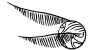
\includegraphics[scale=0.4]{boccino.png}
        \centering
\end{figure}

Giovedì.

A voler essere precisi, le 15:32 di giovedì pomeriggio.

Harry e gli altri ragazzi del primo anno erano all’aperto su di un campo erboso, con Madam Hooch, in piedi di fianco al parco manici di scopa di Hogwarts. Le ragazze avrebbero imparato a volare separatamente. Apparentemente, per qualche ragione, le ragazze non volevano imparare a volare sui manici di scopa in presenza dei ragazzi.

Harry era stato un po’ incerto tutto il giorno. Semplicemente non poteva smettere di chiedersi come quel particolare ciclo temporale stabile fosse stato selezionato all’interno di quello che, in retrospettiva, era un vasto spazio delle possibilità.

E poi: sul serio, manici di scopa? Stava per volare, in pratica, su di un segmento di linea? Non era fondamentalmente la singola forma più instabile che fosse possibile trovare, a meno di non tentare di reggersi su di una biglia puntiforme? Chi aveva scelto quel progetto per un dispositivo per il volo, tra tutte le possibilità? Harry aveva sperato che si trattasse solo di un modo di dire, ma no, erano in piedi di fronte a quelli che sarebbero sembrati a chiunque degli ordinari manici di scopa da cucina in legno. Qualcuno si era semplicemente fissato sull’idea dei manici di scopa e non era riuscito a prendere in considerazione nient’altro? Doveva essere così. Non era proprio possibile che gli strumenti ottimali per pulire una cucina e per andarsene in giro volando coincidessero per caso, se qualcuno ci avesse lavorato sopra ripartendo da zero.

Era una giornata limpida con un cielo blu luminoso e un sole brillante che stava semplicemente pregando di finirti negli occhi e renderti impossibile vedere, se stavi cercando di volartene per quel cielo. Il terreno era bello e asciutto, con un odore come se fosse stato cotto, e in qualche modo sembrava molto, molto duro sotto le scarpe di Harry.

Harry continuò a ricordare a sé stesso che ci si aspettava che il minimo comune denominatore degli undicenni imparasse quella lezione, e che non poteva essere così difficile.

«Allungate la vostra mano destra sul manico, o la sinistra se siete mancini», disse ad alta voce Madam Hooch. «E dite, su!»

«su!» gridarono tutti.

Il manico di scopa saltò impaziente nella mano di Harry.

Cosa che lo rese il primo della classe, per una volta. Apparentemente dire «su!» era molto più difficile di quanto sembrasse, e la maggior parte dei manici stavano rotolandosi per terra o cercando di allontanarsi lentamente dal proprio aspirante pilota.

(Naturalmente Harry avrebbe scommesso dei soldi che Hermione aveva fatto almeno altrettanto bene, quando era stato il suo turno di provare, in precedenza quella stessa mattina. Non era possibile che esistesse qualcosa che egli potesse padroneggiare al primo tentativo e che avrebbe messo in difficoltà Hermione, e se fosse esistito e fosse risultato essere il volo con i manici di scopa invece di qualcosa di intellettuale, Harry ne sarebbe semplicemente morto.)

Ci volle un po’ prima che tutti riuscissero ad avere un manico di scopa di fronte a sé. Madam Hooch mostrò loro come montare e poi girò per il campo a piedi, correggendo impugnature e posizioni. A quanto pareva, anche ai pochi bambini che erano stati autorizzati a volare a casa non era stato insegnato a farlo correttamente.

Madam Hooch osservò il campo pieno di ragazzi e annuì. «Ora, quando soffierò nel fischietto, voi darete un calcio al terreno, forte.»

Harry deglutì, cercando di sedare la sensazione di nausea allo stomaco.

«Stringete fermamente i manici, alzatevi di pochi piedi, e poi tornate subito giù piegandovi leggermente in avanti. Al mio fischio — tre — due –»

Uno dei manici partì sparato verso il cielo, accompagnato dalle urla di un giovane ragazzo — urla di orrore, non di delizia. Il ragazzo stava ruotando a una velocità terribile mentre saliva, e poterono vedere solo di sfuggita il suo volto bianco –

Come fosse al rallentatore, Harry stava saltando giù dal proprio manico di scopa e cercando a tastoni la propria bacchetta, sebbene non sapesse realmente cosa volesse farci, aveva avuto esattamente due lezioni di Incantesimi, e l’ultima era stata sull’Incantesimo di Levitazione, ma Harry era stato in grado di lanciare l’incantesimo solo una volta su tre e certamente non era in grado di far levitare intere persone –

Se esiste un qualunque potere nascosto in me, che si riveli ora!

«Torna indietro, ragazzo!» urlò Madam Hooch (si doveva trattare dell’ordine più inutile che si potesse immaginare per domare un manico di scopa fuori controllo, e proveniva da un istruttore di volo, e una sezione completamente automatizzata del cervello di Harry aggiunse Madam Hooch alla sua lista dei folli).

E il ragazzo fu disarcionato dal manico di scopa.

Sembrò muoversi per aria molto lentamente, all’inizio.

«Wingardium Leviosa!» urlò Harry.

L’incantesimo fallì. Poté percepirlo mentre falliva.

Ci fu un tunf e il suono distante di qualcosa che si rompeva, e il povero ragazzo giacque rattrappito a faccia in giù nell’erba.

Harry rinfoderò la bacchetta e corse avanti alla massima velocità. Arrivò a fianco al ragazzo contemporaneamente a Madam Hooch, infilò la mano nella borsa e cercò di richiamare oh dio come si chiamava non fa niente avrebbe semplicemente provato «Pacchetto di Guarigione!» e gli comparve in mano e –

«Polso fratturato», disse Madam Hooch. «Calmati, ragazzo, ha solo un polso fratturato!»

Vi fu una sorta di sbandamento mentale quando la mente di Harry si riprese dalla Modalità Panico.

Il Pacchetto Extra di Guarigione di Emergenza giaceva aperto di fronte a lui, e in mano a Harry c’era una siringa di fuoco liquido, che sarebbe stato in grado di mantenere ossigenato il cervello del ragazzo nel caso in cui si fosse rotto il collo.

«Ah…» fece Harry con una voce piuttosto incerta. Il suo cuore stava battendo così forte che quasi non riusciva a sentirsi ansimare. «Ossa rotte… va bene… Filo da Sutura?»

«Quello è solo per le emergenze», reagì bruscamente Madam Hooch. «Mettilo via, sta bene.» Si piegò sul ragazzo, offrendogli una mano. «Forza, ragazzo, va tutto bene, alzati!»

«Non avrà seriamente intenzione di farlo salire ancora su quel manico?» chiese Harry inorridito.

Madam Hooch gli lanciò un’occhiataccia. «Naturalmente no!» Sollevò il ragazzo in piedi usando il suo braccio sano — Harry vide con turbamento che si trattava ancora una volta di Neville Longbottom, ma cosa aveva quel ragazzo? — e tornò verso tutti gli altri bambini che stavano guardando. «Nessuno di voi deve muoversi mentre porto questo ragazzo all’ospedale! Lasciate i manici dove sono o sarete fuori da Hogwarts prima che possiate dire ‘Quidditch’. Forza, caro.»

E Madam Hooch si allontanò con Neville, che si stava stringendo il polso e cercava di controllare i singhiozzi.

Quando furono abbastanza lontani, uno dei Serpeverde iniziò a ridacchiare.

Questo diede il la agli altri.

Harry si voltò e li guardò. Sembrò un’ottima occasione per memorizzare alcune facce.

E Harry vide che Draco stava passeggiando verso di lui, accompagnato dal signor Crabbe e dal signor Goyle. Il signor Crabbe non stava sorridendo. Il signor Goyle decisamente sì. Draco stesso aveva un’espressione controllata che occasionalmente si contorceva, da cui Harry dedusse che Draco pensava che la situazione fosse spassosa ma non vedeva come guadagnare alcun vantaggio politico ridendone ora invece che dopo nel sotterraneo dei Serpeverde.

«Insomma, Potter», disse Draco in una voce bassa che non era udibile da lontano, ancora con quell’espressione molto controllata che occasionalmente si contorceva, «Volevo semplicemente dirti, quando sfrutti un’emergenza per fare sfoggio della tua capacità di capo, vuoi che sembri che la situazione sia sotto il tuo controllo, piuttosto che, diciamo, farti prendere dal panico più completo.» Il signor Goyle ridacchiò, e Draco gli lanciò uno sguardo di reprimenda. «Nonostante ciò probabilmente hai ottenuto qualche vantaggio, comunque. Hai bisogno di aiuto per mettere via la cassetta di pronto soccorso?»

Harry si voltò a guardare il Pacchetto di Guarigione, cosa che gli fece distogliere lo sguardo da Draco. «Penso di farcela», disse Harry. Mise la siringa al suo posto, riannodò i lacci, e si alzò.

Ernie Macmillan arrivò proprio mentre Harry stava inserendo il pacchetto nella sua borsa mokeskin.

«Grazie, Harry Potter, a nome dei Tassofrasso», disse formalmente Ernie Macmillan. «È stato un buon tentativo e una buona idea.»

«Una buona idea davvero», disse Draco strascicando le parole. «Perché i Tassofrasso non hanno tutti estratto le bacchette? Forse se tutti voi aveste aiutato, invece del solo Potter, avreste potuto prenderlo. Pensavo che i Tassofrasso dovessero aiutarsi a vicenda.»

Ernie sembrò diviso tra l’arrabbiarsi e il voler morire di vergogna. «Non ci abbiamo pensato in tempo –»

«Ah», disse Draco, «non ci avete pensato, credo che sia per questo che è meglio avere un Corvonero per amico che tutti i Tassofrasso.»

Oh, al diavolo, come avrebbe dovuto destreggiarsi in tutto ciò Harry… «Non sei d’aiuto», disse in tono mite. Sperando che Draco l’avrebbe interpretato come stai interferendo nei miei piani, per favore taci.

«Ehi, cos’è questa?» chiese il signor Goyle. Si chinò sull’erba e raccolse qualcosa dalle dimensioni simili a una grossa biglia, una palla di vetro che sembrava piena di una vorticante nebbiolina bianca.

Ernie sbatté le palpebre. «La Ricordella di Neville!»

«Cos’è una Ricordella?» chiese Harry.

«Diventa rossa se ti sei dimenticato qualcosa», rispose Ernie. «Non ti dice cosa hai dimenticato, però. Dalla a me, per favore, la restituirò a Neville più tardi.» Ernie tese la mano.

Un’improvviso ghigno balenò sul volto del signor Goyle, che si girò e corse via.

Ernie rimase fermo un momento per la sorpresa, poi gridò «Ehi!» e corse dietro al signor Goyle.

E il signor Goyle afferrò un manico di scopa, vi saltò sopra con un unico movimento fluido e si alzò in aria.

Harry rimase sconvolto. Madam Hooch non aveva detto che quello avrebbe causato la sua espulsione?

«Quell’idiota!» sibilò Draco. Aprì la bocca per gridare –

«Ehi!» urlò Ernie. «Quella è di Neville! Restituiscila!»

I Serpeverde iniziarono ad acclamare e a fischiare.

La bocca di Draco si chiuse di colpo. Harry colse l’improvvisa espressione di indecisione sul suo volto.

«Draco», chiamò Harry a bassa voce, «se non ordini a quell’idiota di tornare a terra, l’insegnante tornerà e –»

«Venitevela a prendere, Tassofrasso!» gridò il signor Goyle, e una grande acclamazione si alzò dai Serpeverde.

«Non posso!» sussurrò Draco. «Tutti i Serpeverde penseranno che sono debole!»

«E se il signor Goyle si fa espellere», sibilò Harry, «tuo padre penserà che sei un imbecille!»

Il volto di Draco si deformò per l’agonia.

In quel momento –

«Ehi, Serpemarcia», gridò Ernie, «nessuno ti ha mai detto che i Tassofrasso restano uniti? Mano alle bacchette, Tassofrasso!»

E ci fu improvvisamente un gran numero di bacchette puntate nella direzione del signor Goyle.

Tre secondi dopo –

«Mano alle bacchette, Serpeverde!» dissero circa cinque diversi Serpeverde.

E ci fu un gran numero di bacchette puntate nella direzione dei Tassofrasso.

Due secondi dopo –

«Mano alle bacchette, Grifondoro!»

«Fa’ qualcosa, Potter!» bisbigliò Draco. «Non posso essere io a fermarli, devi essere tu! Ti dovrò un favore, pensa a qualcosa, non dovresti essere geniale?»

In circa cinque secondi e mezzo, capì Harry, qualcuno avrebbe lanciato la Fattura d’Attacco Semplice Sumera e quando tutto fosse terminato e i professori avessero finito di espellere studenti, gli unici ragazzi rimasti del suo anno sarebbero stati i Corvonero.

«Mano alle bacchette, Corvonero!» gridò Michael Corner, che apparentemente si sentiva lasciato fuori dal disastro.

«gregory goyle!» urlò Harry. «Ti sfido a una competizione per il possesso della Ricordella di Neville!»

Ci fu un’improvvisa pausa.

«Oh, davvero?» disse Draco nella parlata annoiata più alta che Harry avesse mai sentito. «Sembra interessante. Che tipo di competizione, Potter?»

Ehm…

«Competizione» era il massimo che l’ispirazione di Harry avesse prodotto. Che tipo di competizione, non avrebbe potuto dire «scacchi» perché Draco non sarebbe stato in grado di accettare senza sembrare strano, non poteva dire «braccio di ferro» perché il signor Goyle l’avrebbe schiacciato –

«Che ne dite di questo?» Harry disse ad alta voce. «Gregory Goyle e io ce ne stiamo in piedi, distanti l’uno dall’altro, e a nessuno è permesso avvicinarsi a noi. Non usiamo le nostre bacchette e nessun altro lo fa. Non mi muovo da dove sono, e non lo fa neppure lui. E se riesco a mettere le mani sulla Ricordella di Neville, allora Gregory Goyle rinuncia a tutte le sue pretese sulla Ricordella che tiene in mano e la dà a me.»

Ci fu un’altra pausa mentre le espressioni di sollievo si tramutavano in confusione.

«Aha, Potter!» disse Draco ad alta voce. «Voglio proprio vedertelo fare! Il signor Goyle accetta!»

«Andata!» disse Harry.

«Potter, cosa diavolo?» bisbigliò Draco, riuscendoci, in qualche modo, senza muovere le labbra.

Harry non sapeva come rispondere senza muovere le sue.

Iniziarono tutti a mettere via le bacchette, e il signor Goyle discese repentinamente al suolo con grazia, l’espressione alquanto confusa. Alcuni Tassofrasso iniziarono a muoversi verso il signor Goyle, ma Harry lanciò loro uno sguardo di disperata preghiera, ed essi si fermarono.

Harry si diresse verso il signor Goyle e si fermò quando si trovarono a pochi passi di distanza, abbastanza lontani da non potersi raggiungere l’un l’altro.

Lentamente, deliberatamente, Harry ripose la bacchetta.

Tutti gli altri indietreggiarono.

Harry deglutì. Sapeva a grandi linee quello che voleva fare, ma doveva essere realizzato in modo tale che nessuno capisse cosa aveva fatto –

«Va bene», disse Harry a voce alta. «E ora…» Fece un respiro profondo e alzò una mano, le dita pronte a schioccare. Ci furono rantoli emessi da chiunque avesse sentito parlare delle torte, ovvero praticamente tutti. «Invoco la follia di Hogwarts! Felice felice bum bum palude palude palude!» E Harry schioccò le dita.

Parecchi trasalirono.

E nulla accadde.

Harry lasciò che il silenzio si allungasse per un po’, crescendo, finché…

«Uhm», fece qualcuno. «Tutto qui?»

Harry guardò il ragazzo che aveva parlato. «Guarda davanti a te. Vedi quella zona di terra che sembra spoglia, senza erba sopra?»

«Uhm, sì», disse il ragazzo, un Grifondoro (Dean qualcosa?).

«Scava lì.»

Adesso Harry ricevette parecchie occhiate strane.

«Ehm, perché?» disse Dean qualcosa.

«Fallo e basta», rispose Terry Boot, con la voce stanca. «È inutile chiedere perché, fidatevi.»

Dean qualcosa si inginocchiò e cominciò a scavare per terra.

Dopo un minuto o giù di lì, Dean si alzò di nuovo. «Non c’è niente qui.»

Ah. Harry aveva avuto intenzione di tornare indietro nel tempo e di seppellire una mappa del tesoro che avrebbe portato a un’altra mappa del tesoro che avrebbe portato alla Ricordella di Neville, che avrebbe messo lì dopo averla ottenuta indietro dal signor Goyle…

Poi Harry si rese conto che c’era un modo molto più semplice che non minacciava di rivelare il segreto del Giratempo allo stesso modo.

«Grazie, Dean!» disse Harry a voce alta. «Ernie, daresti un’occhiata al terreno dove Neville è caduto per vedere se è possibile ritrovare la sua Ricordella?»

Tutti sembrarono ancora più confusi.

«Fallo e basta» disse Terry Boot. «Continuerà così finché qualcosa non funzionerà, e la cosa peggiore è che –»

«Merlino!» rantolò Ernie. Reggeva la Ricordella di Neville. «È qui! Proprio dov’è caduto!»

«Cosa?» gridò il signor Goyle. Guardò in basso e vide…

… che stava ancora reggendo la Ricordella di Neville.

Ci fu una pausa piuttosto lunga.

«Ehm», disse Dean qualcosa, «questo non è possibile, giusto?»

«È un’inconsistenza nella trama», disse Harry. «Mi sono reso abbastanza strano da distrarre l’universo per un momento, ed esso ha dimenticato che Goyle aveva già raccolto la Ricordella.»

«No, aspetta, voglio dire, questo non è assolutamente possibile –»

«Scusami, siamo tutti quanti qui aspettando di iniziare a volare su manici di scopa? Sì, lo siamo. Quindi taci. Ad ogni modo, una volta che metto le mani sulla Ricordella di Neville, la competizione è terminata e Gregory Goyle deve rinunciare a ogni pretesa sulla Ricordella che sta tenendo e darla a me. Questi erano i termini, ricordate?» Harry allungò una mano e fece un cenno a Ernie. «Falla semplicemente rotolare qui, poiché nessuno deve avvicinarsi a me, va bene?»

«Fermi tutti!» gridò un Serpeverde — Blaise Zabini, Harry avrebbe difficilmente dimenticato quel nome. «Come facciamo a sapere che quella è la Ricordella di Neville? Potresti aver semplicemente lasciato cadere lì un’altra Ricordella –»

«Serpeverde è forte in lui», disse Harry, sorridendo. «Ma hai la mia parola che quella che Ernie sta tenendo è di Neville. Nulla affermo a proposito di quella che è in possesso di Gregory Goyle.»

Zabini si girò verso Draco. «Malfoy! Non avrai intenzione di permettergli di cavarsela così –»

«Chiudi quella bocca, tu» rimbombò il signor Crabbe, in piedi dietro Draco. «Il signor Malfoy non ha bisogno che tu gli dica cosa fare!»

Bravo servitore.

«La mia scommessa era con Draco, della Nobile e Antichissima Casa Malfoy», disse Harry. «Non con te, Zabini. Ho fatto quello che il signor Malfoy ha detto gli sarebbe piaciuto vedermi fare, e per quanto riguarda il verdetto sulla scommessa, lo lascio nelle mani del signor Malfoy.» Harry inclinò la testa verso Draco e inarcò leggermente le sopracciglia. Questo avrebbe dovuto consentire a Draco di salvare sufficientemente la faccia.

Ci fu una pausa.

«Prometti che quella è effettivamente la Ricordella di Neville?» disse Draco.

«Sì», rispose Harry. «Quella è la Ricordella che ritornerà a Neville e che fu originariamente sua. E quella che Gregory Goyle sta tenendo va a me.»

Draco annuì, l’espressione risoluta. «Non metterò in dubbio la parola della Nobile Casa Potter, allora, non importa quanto strano sia tutto questo. E allo stesso modo la Nobile e Antichissima Casa Malfoy mantiene la propria parola. Signor Goyle, la dia al signor Potter –»

«Ehi!» disse Zabini. «Non ha ancora vinto, non ha ancora messo le mani su –»

«Prendi, Harry!» disse Ernie, e lanciò la Ricordella.

Harry prese facilmente al volo la Ricordella, aveva sempre avuto buoni riflessi. «Ecco», disse, «ho vinto…»

La voce di Harry si affievolì. Tutte le conversazioni si fermarono.

Nella sua mano la Ricordella stava brillando di un rosso intenso, ardendo come un sole in miniatura che getta ombre sul terreno nella piena luce del giorno.

\begin{figure}[h!]
        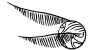
\includegraphics[scale=0.4]{boccino.png}
        \centering
\end{figure}

Giovedì.

A voler essere precisi, le 17:09 di giovedì pomeriggio, nell’ufficio della professoressa McGonagall, dopo le lezioni di volo (con un’ulteriore ora inserita in mezzo per Harry).

La professoressa McGonagall sedeva sul suo sgabello. Harry nella sedia dell’imputato di fronte alla sua scrivania.

«Professoressa», disse Harry con fermezza, «i Serpeverde stavano puntando le loro bacchette contro i Tassofrasso, i Grifondoro stavano puntando le loro bacchette contro i Serpeverde, qualche idiota ha ordinato ai Corvonero di estrarre le bacchette, e io ho avuto forse cinque secondi per impedire all’intera faccenda di esplodere! È stato tutto quello che sono riuscito a pensare!»

Il volto della professoressa McGonagall era emaciato e infuriato. «Non deve usare il Giratempo in quel modo, signor Potter! Le è forse difficile comprendere il concetto di segretezza?»

«Non sanno come ho fatto! Pensano solo che io possa fare cose veramente bizzarre schioccando le dita! Ho fatto anche altre cose bizzarre che non possono essere realizzate con i Giratempo, e farò altre cose di questo genere, e questo caso non sarà neppure ricordato! Dovevo farlo, professoressa!»

«Lei non aveva bisogno di farlo!» scattò la professoressa McGonagall. «Tutto ciò che doveva fare era era portare questo Serpeverde anonimo a terra e deporre le bacchette! Avrebbe potuto sfidarlo a una partita di Spara Schiocco, ma no, lei doveva usare il Giratempo in maniera plateale e inutile!»

«È stato tutto quello che sono riuscito a pensare! Non so neppure cosa sia Spara Schiocco, non avrebbero acconsentito a una partita a scacchi e se avessi scelto braccio di ferro avrei perso!»

«Allora avrebbe dovuto scegliere braccio di ferro!»

Harry sbatté le palpebre. «Ma allora avrei perso –»

Si fermò.

La professoressa McGonagall sembrava davvero arrabbiata.

«Mi dispiace, professoressa McGonagall», disse Harry a bassa voce. «Onestamente non ci ho pensato, e lei ha ragione, avrei dovuto, sarebbe stato geniale se l’avessi fatto, ma non ci ho neppure pensato…»

La voce di Harry si spense. Gli fu improvvisamente chiaro che aveva avuto molte altre opzioni. Avrebbe potuto chiedere a Draco di suggerire qualcosa, avrebbe potuto chiedere alla folla… il suo uso del Giratempo era stato plateale e inutile. Aveva avuto a disposizione un gigantesco spazio delle possibilità, perché aveva scelto quella?

Perché aveva visto un modo per vincere. Vincere il possesso di un gingillo che gli insegnanti avrebbero comunque tolto al signor Goyle.

La volontà di vincere. Si era impadronita di lui.

«Mi dispiace», disse ancora Harry. «Per il mio orgoglio e per la mia stupidità.»

La professoressa McGonagall si passò una mano sulla fronte. Parte della sua rabbia sembrò svanire. Ma la voce venne fuori ancora molto dura. «Un’altra esibizione come questa, signor Potter, e restituirà il Giratempo. Sono stata chiara?»

«Sì», rispose Harry. «Comprendo e mi dispiace.»

«Allora, signor Potter, le sarà permesso tenere il Giratempo, per ora. E considerando le dimensioni del disastro che è riuscito, in conclusione, a evitare, non detrarrò alcun punto a Corvonero.»

Per di più non avrebbe potuto spiegare perché avesse detratto i punti. Ma Harry non era sufficientemente sciocco da dirlo a voce alta.

«Soprattutto, perché la Ricordella si è accesa in quel modo?» chiese Harry. «Significa che sono stato Obliato?»

«Questo lascia perplessa anche me», disse lentamente la professoressa McGonagall. «Se fosse così semplice, credo che i tribunali utilizzerebbero le Ricordelle, e non lo fanno. Dovrò investigare la faccenda, signor Potter.» Sospirò. «Ora può andare.»

Harry iniziò ad alzarsi dalla sedia, poi si fermò. «Uhm, mi scusi, avevo qualcos’altro da chiederle –»

Poté notare a malapena il sussulto. «Di che si tratta, signor Potter?»

«Del professor Quirrell –»

«Sono certa, signor Potter, che non sia nulla di importante.» La professoressa McGonagall pronunciò le parole con molta fretta. «Sicuramente ha udito il Preside dire agli studenti che non dovete disturbarci con lamentele di scarsa importanza riguardo il Professore di Difesa.»

Harry era piuttosto confuso. «Ma questo potrebbe essere importante, ieri ho percepito questa improvvisa sensazione di sventura quando –»

«Signor Potter! Anche io ho una sensazione di sventura! E la mia sensazione di sventura mi suggerisce che lei non debba terminare quella frase!»

La bocca di Harry si spalancò. La professoressa McGonagall aveva avuto successo; Harry era senza parole.

«Signor Potter», disse la professoressa McGonagall, «se ha scoperto qualunque cosa che le sembra importante riguardo il professor Quirrell, la prego, si senta libero di non condividerla con me o con chiunque altro. Ora credo che abbia impegnato a sufficienza il mio tempo prezioso –»

«Questo non è da lei!» scoppiò Harry. «Mi dispiace, ma questo mi sembra incredibilmente irresponsabile! Da quanto ho sentito c’è una specie di maledizione sulla cattedra di Difesa, e se sapeste già che qualcosa andrà male, credo che sareste tutti in allerta –»

«Andare male, signor Potter? Io certamente spero di no.» Il volto della professoressa McGonagall era senza espressione. «Dopo che la professoressa Blake è stata trovata in uno stanzino con non meno di cinque Serpeverde del quinto anno, lo scorso febbraio, e che un anno prima la professoressa Summers è stata un tale fallimento come educatrice che i suoi studenti credevano che un Molliccio fosse un tipo di mobile, sarebbe catastrofico se qualche problema con lo straordinariamente competente professor Quirrell fosse portato alla mia attenzione ora, e oserei dire che la maggior parte dei nostri studenti fallirebbe i suoi g.u.f.o. in Difesa e i suoi m.a.g.o.»

«Capisco», disse Harry lentamente, meditando il tutto. «Quindi, in altre parole, qualunque cosa ci sia di sbagliato nel professor Quirrell, lei non ne vuole sapere nulla fino alla fine dell’anno scolastico. E poiché siamo a settembre, potrebbe assassinare il Primo Ministro in diretta televisiva e cavarsela, per quanto la riguarda.»

La professoressa McGonagall lo guardò senza battere ciglio. «Sono certa che non potrei mai essere sentita sostenere una posizione del genere, signor Potter. A Hogwarts ci sforziamo di prevenire qualunque cosa minacci i traguardi educativi dei nostri studenti.»

Come i Corvonero del primo anno che non sanno tenere chiusa la bocca. «Credo di capirla perfettamente, professoressa McGonagall.»

«Ne dubito, signor Potter. Ne dubito molto.» La professoressa McGonagall si sporse in avanti, il viso che si fece nuovamente severo. «Poiché lei e io abbiamo già discusso faccende molto più delicate di questa, le parlerò schiettamente. Lei, e solo lei, ha riferito questa sensazione di sventura. Lei, e solo lei, è un magnete per il caos del quale non ho mai visto il simile. Dopo il nostro giro di spese a Diagon Alley, e poi il Cappello Smistatore, e poi il piccolo episodio di oggi, posso ben presagire che sono destinata a stare seduta nell’ufficio del Preside ad ascoltare qualche spassosissima storia a proposito del professor Quirrell in cui lei e solo lei interpreta una parte da protagonista, dopo di che non vi sarà altra scelta che licenziarlo. Sono già rassegnata a questo, signor Potter. E se questo triste evento dovesse avere luogo prima delle Idi di maggio, la appenderò all’ingresso di Hogwarts con i suoi stessi intestini, e verserò delle coccinelle di fuoco nel suo naso. Mi ha capito bene, ora?»

Harry annuì, gli occhi spalancati. Poi, dopo un secondo, «E se potessi farlo accadere l’ultimo giorno di scuola dell’anno?»

«Esca dal mio ufficio!»

\begin{figure}[h!]
        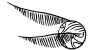
\includegraphics[scale=0.4]{boccino.png}
        \centering
\end{figure}

Giovedì.

Doveva esserci qualcosa di strano a proposito dei giovedì a Hogwarts.

Erano le 17:32 di giovedì pomeriggio, e Harry era in piedi vicino al professor Flitwick, di fronte al grande gargoyle di pietra che faceva la guardia all’ingresso dell’ufficio del Preside.

Dopo essere tornato dall’ufficio della professoressa McGonagall alle sale studio di Corvonero, uno degli studenti gli aveva detto di presentarsi nell’ufficio del professor Flitwick, e lì Harry aveva scoperto che Silente voleva parlargli.

Sentendosi piuttosto ansioso, aveva chiesto al professor Flitwick se il Preside avesse detto di cosa si trattava.

Il professor Flitwick aveva alzato le spalle in maniera impotente.

Apparentemente Silente aveva affermato che Harry era troppo giovane per invocare le parole del potere e della follia.

Felice felice bum bum palude palude palude? Harry aveva pensato ma non detto ad alta voce.

«La prego, non si preoccupi troppo, signor Potter», squittì il professor Flitwick da una qualche parte all’altezza delle spalle di Harry. (Harry era grato per la gigantesca e gonfia barba del professor Flitwick, era difficile abituarsi ad un Professore che non era solo più basso di lui, ma che parlava con un tono più acuto.) «Il preside Silente può sembrare un po’ strano, o molto strano, o anche estremamente strano, ma non ha mai fatto alcun male a uno studente, e non credo lo farà mai.» Il professor Flitwick rivolse a Harry un sorriso di incoraggiamento. «Cerchi di ricordarlo sempre e non si lascerà prendere dal panico!»

Non era d’aiuto.

«Buona fortuna!» squittì il professor Flitwick, si chinò verso il gargoyle e disse qualcosa che Harry, in qualche modo, non sentì neppure. (Ovviamente, la parola d’accesso non sarebbe stata un granché se l’avessi potuta sentire pronunciare.) E il gargoyle di pietra si mosse di lato con un movimento molto naturale e ordinario che Harry trovò alquanto sconvolgente, poiché il gargoyle continuò a sembrare pietra solida e immobile per tutto il tempo.

Dietro il gargoyle si trovava una scala a chiocciola che ruotava lentamente. C’era qualcosa di ipnotico e inquietante in tutto ciò, e ancora più inquietante era il fatto che una scala a chiocciola ruotante non avrebbe dovuto portarti da nessuna parte.

«Salga!» squittì Flitwick.

Harry mise piuttosto nervosamente il piede sulla scala, e si trovò, per qualche ragione che il suo cervello non sembrava affatto in grado di visualizzare, a muoversi verso l’alto.

Il gargoyle dietro di lui tornò al proprio posto con un tonfo, le scale a chiocciola continuarono a ruotare e Harry continuò a essere sempre più in alto, e dopo un periodo piuttosto vertiginoso, Harry si trovò di fronte a una porta di quercia con un grifone battente in ottone.

Harry allungò la mano e girò la maniglia.

La porta si aprì.

E Harry vide la stanza più interessante che avesse mai visto in vita sua.

C’erano minuscoli meccanismi metallici che ronzavano o ticchettavano o cambiavano lentamente forma o emettevano piccoli sbuffi di fumo. C’erano dozzine di fluidi misteriosi in dozzine di contenitori dalla forma strana, tutti gorgoglianti, ribollenti, trasudanti, mutanti colore, o formanti arrangiamenti interessanti che scomparivano mezzo secondo dopo che li avevi notati. C’erano oggetti che sembravano orologi con molte lancette, con numeri incisi o in lingue irriconoscibili. C’era un bracciale con incastonato un cristallo lenticolare che brillava di mille colori, e un uccello appollaiato in cima a una piattaforma d’oro, e una tazza di legno riempita con quello che sembrava sangue, e la statua di un falco incrostato in smalto nero. La parete era tutta tappezzata di immagini di persone dormienti, e il Cappello Smistatore era casualmente attaccato a una cappelliera che stava reggendo anche due ombrelli e tre pantofole rosse per piedi sinistri.

Nel mezzo di tutta quella confusione, stava una semplice scrivania di quercia nera. Davanti alla scrivania c’era uno sgabello di quercia. E dietro la scrivania c’era un trono ben imbottito contenente Albus Percival Wulfric Brian Silente, adorno di una lunga barba d’argento, un cappello simile a fungo gigante schiacciato, e ciò che a occhi babbani sembravano tre strati di pigiama rosa brillante.

Silente stava sorridendo, i suoi occhi luminosi che brillavano di una folle intensità.

Con un po’ di trepidazione, Harry si sedette di fronte alla scrivania. La porta si chiuse da sola dietro di lui con un forte tunc.

«Ciao, Harry», disse Silente.

«Ciao, Preside», rispose Harry. Quindi si davano del tu? Silente gli avrebbe ora detto di chiamarlo –

«Per favore, Harry!» disse Silente. «Preside suona così formale. Chiamami semplicemente Pre, per semplicità.»

«Lo farò senz’altro, Pre», disse Harry.

Ci fu una breve pausa.

«Lo sai», disse Silente, «che sei la prima persona che mi abbia mai preso sul serio su questo punto?»

«Ah…» disse Harry. Cercò di controllare la propria voce malgrado l’improvvisa sensazione di sprofondare. «Mi scusi, io, ah, Preside, lei mi ha detto di farlo e quindi io –»

«Eh, ti prego!» disse Silente allegro. «E non c’è nessun bisogno di essere così preoccupato, non ti lancerò da una finestra solo perché hai fatto un errore. Ti avvertirò a sufficienza, prima, se stai facendo qualcosa di sbagliato! Inoltre, ciò che importa non è come le persone si rivolgono a te, è cosa pensano di te.»

Non ha mai fatto del male a uno studente, continua solo a ricordare questo e non ti farai prendere dal panico.

Silente tirò fuori una scatolina di metallo e l’aprì, mostrando alcuni piccoli grumi gialli. «Frizlemon?», disse il Preside.

«Ehm, no, grazie, eh», disse Harry. Somministrare lsd a uno studente conta come fargli del male, o ricade nella categoria innocuo divertimento? «Lei ha, uhm, detto qualcosa a riguardo del fatto che sarei troppo giovane per invocare le parole del potere e della follia?»

«Che lo sei con assoluta certezza!» rispose Silente. «Fortunatamente le Parole del Potere e della Follia furono smarrite sette secoli fa e nessuno ha più la minima idea di quali siano. Era semplicemente una piccola osservazione.»

«Ah…» disse Harry. Era cosciente del fatto che la sua bocca fosse rimasta aperta. «Allora perché mi ha chiamato qui?»

«Perché?» rispose Silente. «Ah, Harry, se andassi in giro tutto il giorno chiedendomi perché faccio le cose, non avrei mai il tempo per fare una singola cosa! Sono una persona alquanto impegnata, sai.»

Harry annuì, sorridendo. «Sì, era una lista molto impressionante. Preside di Hogwarts, Stregone Capo del Wizengamot, e Supremo Pezzo Grosso della Confederazione Internazionale dei Maghi. Scusi la domanda, ma mi chiedevo, è possibile ricevere più di sei ore se si usano più Giratempo? Perché è abbastanza impressionante se sta facendo tutto con appena 30 ore in un giorno.»

Ci fu un’altra breve pausa, durante la quale Harry continuò a sorridere. Era un po’ ansioso, in realtà molto ansioso, ma una volta chiaro che Silente stava deliberatamente cercando di confonderlo, qualcosa dentro di lui si rifiutò assolutamente di restare seduto a subire come una vittima predestinata.

«Ho paura che il Tempo non gradisca troppo essere stiracchiato», disse Silente dopo la breve pausa, «eppure noi stessi sembriamo un po’ troppo grossi per lui, e quindi è una lotta continua per far calzare le nostre vite all’interno del Tempo.»

«Infatti», disse Harry con profonda solennità. «Ecco perché è meglio arrivare direttamente alle nostre questioni.»

Per un momento Harry si chiese se avesse esagerato.

Poi Silente ridacchiò. «E dritti al punto sia.» Il Preside si chinò in avanti, inclinando il cappello a fungo schiacciato e spazzolando la barba contro la scrivania. «Harry, questo lunedì hai fatto qualcosa che avrebbe dovuto essere impossibile anche con un Giratempo. O meglio, impossibile con solo un Giratempo. Da dove sono giunte quelle due torte, mi chiedo?»

Un’ondata di adrenalina attraversò Harry. L’aveva fatto usando il Mantello dell’Invisibilità, quello che gli era stato dato in un pacco natalizio insieme a una nota, e quella nota aveva detto: se Silente intravvedesse la possibilità di possedere uno dei Doni della Morte non se la farebbe scappare…

«Un pensiero naturale», continuò Silente, «è che siccome nessuno degli studenti del primo anno presenti era in grado di lanciare un incantesimo di questo tipo, qualcun altro fosse presente, sebbene non visto. E se nessuno avesse potuto vederlo, ebbene, sarebbe stato facile per lui lanciare le torte. Si potrebbe ulteriormente sospettare che siccome tu avevi un Giratempo, fossi tu quello invisibile; e che poiché l’incantesimo di Disillusione è molto al di là delle tue attuali capacità, tu fossi in possesso di un mantello invisibile.» Silente gli rivolse un sorriso complice. «Sono sulla buona strada finora, Harry?»

Harry era paralizzato. Aveva la sensazione che una pura e semplice bugia non sarebbe stata saggia, e forse neppure utile, e non riuscì a pensare a nient’altro da dire.

Silente agitò la mano in maniera amichevole. «Non preoccuparti, Harry, non hai fatto niente di male. I mantelli invisibili non sono contro le regole — suppongo che siano talmente rari che nessuno si sia mai preoccupato di inserirli nell’elenco. Ma in realtà mi chiedevo qualcosa di completamente diverso.»

«Oh?» disse Harry con la voce più normale che gli riuscisse.

Gli occhi di Silente brillavano di entusiasmo. «Vedi, Harry, dopo che hai avuto una manciata di avventure, tendi a capire l’essenza di queste faccende. Inizi a vedere lo schema, a sentire il ritmo del mondo. Cominci ad albergare sospetti prima del momento della rivelazione. Tu sei il Ragazzo-Che-È-Sopravvissuto, e in qualche modo un mantello invisibile si è fatto strada fino alle tue mani appena quattro giorni dopo che hai scoperto la nostra Gran Bretagna magica. Tali mantelli non sono in vendita a Diagon Alley, ma ce n’è uno che potrebbe trovare la propria strada fino a un possessore predestinato. E così non posso fare a meno di chiedermi se per qualche strano caso hai trovato non solo un mantello invisibile, ma il Mantello dell’Invisibilità, uno dei tre Doni della Morte e ritenuto in grado di nascondere chi lo indossa dagli sguardi della Morte stessa.» Lo sguardo di Silente era luminoso e impaziente. «Posso vederlo, Harry?»

Harry deglutì. Ora c’era un’alta marea di adrenalina dentro di lui ed era del tutto inutile, quello era il mago più potente del mondo ed era impossibile che potesse raggiungere la porta e non c’era alcun luogo a Hogwarts dove potesse nascondersi se ci fosse riuscito, stava per perdere il Mantello che era stato tramandato dai Potter per chissà quanto tempo –

Lentamente Silente si sedette nuovamente nel suo trono. La luce era scomparsa dai suoi occhi, e sembrò perplesso e un po’ triste. «Harry», disse, «se vuoi, puoi semplicemente dire di no.»

«Posso?» disse Harry con voce rauca.

«Sì, Harry», disse Silente. La sua voce suonava triste, ora, e preoccupata. «Sembra che tu abbia paura di me, Harry. Posso chiedere che cosa ho fatto per guadagnare la tua diffidenza?»

Harry deglutì. «C’è qualche modo in cui può pronunciare un giuramento magico vincolante che non prenderà il mio mantello?»

Silente scosse lentamente la testa. «I Voti Infrangibili non devono essere presi così alla leggera. E poi, Harry, se non conosci già l’incantesimo, avresti solo la mia parola che l’incantesimo fosse vincolante. Ma sicuramente ti rendi conto che non ho bisogno del tuo permesso per vedere il Mantello. Sono abbastanza potente per prenderlo io stesso, borsa mokeskin o meno.» Il volto di Silente era molto severo. «Ma non lo farò. Il Mantello è tuo, Harry. Non voglio sottrartelo. Nemmeno per guardarlo solo per un momento, a meno che non sia tu a decidere di mostrarmelo. Questa è una promessa e un giuramento. Dovessi avere il bisogno di proibirtene l’utilizzo all’interno della scuola, pretenderei che andassi alla tua camera blindata presso Gringotts e lo depositassi lì.»

«Ah…» disse Harry. Deglutì a fatica, cercando di calmare l’ondata di adrenalina e di pensare in maniera ragionevole. Prese la borsa mokeskin dalla cintura. «Se davvero non ha bisogno del mio permesso… allora lo prenda.» Harry porse la borsa a Silente, e si morse con forza il labbro, inviando un segnale a sé stesso nel caso in cui fosse stato successivamente Obliato.

Il vecchio mago infilò la mano nel sacchetto, e senza pronunciare alcuna parola di recupero, estrasse il Mantello dell’Invisibilità.

«Ah», inspirò Silente. «Avevo ragione…» Fece scivolare sulla mano la cangiante trama vellutata e nera. «Vecchio di secoli, e ancora perfetto come il giorno in cui fu realizzato. Abbiamo perso gran parte della nostra arte nel corso degli anni, e ora io stesso non posso creare una cosa del genere, nessuno può. Riesco a sentirne il potere come un eco nella mia mente, come una canzone cantata per sempre senza nessuno che l’ascolti…» Il mago alzò lo sguardo dal Mantello. «Non venderlo», disse, «non trasferirne il possesso a nessuno. Pensaci due volte prima di mostrarlo a chicchessia, e pensaci tre volte prima di rivelare che si tratta di uno dei Doni della Morte. Trattalo con rispetto, perché questo è davvero un Oggetto di Potere.»

Per un attimo il volto di Silente divenne malinconico…

… e poi consegnò nuovamente il Mantello a Harry.

Harry lo rimise nella proprio borsa.

Il volto di Silente fu ancora una volta serio. «Posso chiedere di nuovo, Harry, come sei arrivato a diffidare in questo modo di me?»

All’improvviso Harry si sentì piuttosto imbarazzato.

«C’era una nota con il Mantello», disse Harry a bassa voce. «Diceva che lei avrebbe cercato di prendermi il Mantello, se avesse saputo. Non so chi abbia lasciato la nota, però, davvero non lo so».

«Io… capisco» disse Silente lentamente. «Bene, Harry, non voglio mettere in dubbio le motivazioni di chi ti ha lasciato questa nota. Chi lo sa, magari potrebbe aver avuto la migliore delle intenzioni, giusto? Ti ha dato il Mantello, dopo tutto.»

Harry annuì, colpito dall’indulgenza di Silente, e imbarazzato dal netto contrasto con il proprio atteggiamento.

Il vecchio mago continuò. «Ma tu e io siamo entrambi pezzi da gioco dello stesso colore, credo. Il ragazzo che finalmente sconfisse Voldemort, e il vecchio che lo tenne impegnato per un tempo sufficiente a permetterti di risolvere il problema. Non ce l’avrò con te per la tua cautela, Harry, noi tutti dobbiamo fare del nostro meglio per essere saggi. Mi limiterò a chiedere che tu pensi due volte e mediti di nuovo tre volte, la prossima volta che qualcuno ti dirà di diffidare di me.»

«Mi dispiace», disse Harry. In quel momento si sentiva miserabile, aveva appena rimproverato Gandalf, essenzialmente, e la gentilezza di Silente lo stava solo facendo sentire peggio. «Non avrei dovuto diffidare di lei.»

«Ahimè, Harry, in questo mondo…» L’anziano mago scosse la testa. «Non posso neppure dire che sei stato imprudente. Non mi conoscevi. E in verità vi sono alcuni a Hogwarts di cui faresti bene a non fidarti. Forse anche alcuni che chiami amici.»

Harry deglutì. Questo sembrava piuttosto sinistro. «Come chi?»

Silente si alzò dalla sedia, e cominciò a esaminare uno dei suoi strumenti, un quadrante con otto lancette di lunghezza differente.

Dopo pochi istanti, il vecchio mago parlò di nuovo. «Probabilmente ti sembra alquanto affascinante», disse Silente. «Garbato — con te, almeno. Ben educato, forse ti ammira, persino. Sempre pronto a dare una mano, un favore, una parola di consiglio –»

«Oh, Draco Malfoy!» disse Harry, sentendosi piuttosto sollevato dal fatto che non fosse Hermione o qualcosa del genere. «Oh no, no no no, ha capito male, lui non sta convertendo me, io sto convertendo lui.»

Silente si fermò lì dov’era, mentre scrutava il quadrante. «Stai facendo cosa?»

«Ho intenzione di allontanare Draco Malfoy dal Lato Oscuro», disse Harry. «Ha presente, farne un bravo ragazzo.»

Silente si raddrizzò e si voltò verso Harry. Aveva una delle espressioni più attonite che Harry avesse mai visto su chiunque, tanto più su qualcuno con una lunga barba d’argento. «Sei certo», disse il vecchio mago dopo un momento, «che è pronto per essere redento? Temo che qualunque bontà tu veda in lui sia solo un pio desiderio — o peggio, un richiamo, un’esca –»

«Ehm, improbabile», disse Harry. «Voglio dire, se sta cercando di farsi passare per bravo ragazzo è incredibilmente incompetente. Questa non è la situazione in cui Draco mi si avvicina e si comporta in maniera affabile e io decido che deve avere un nucleo di bontà nascosto in profondità. Ho scelto di redimere lui proprio perché è l’erede di Casa Malfoy e se dovessi scegliere una persona da redimere, sarebbe ovviamente lui.»

L’occhio sinistro di Silente ebbe una contrazione. «Hai intenzione di piantare i semi dell’amore e della gentilezza nel cuore di Draco Malfoy perché ti aspetti che l’erede di Malfoy si dimostri prezioso per te?»

«Non solo per me!» disse Harry indignato. «Per l’intera Gran Bretagna magica, se questo funziona! E inoltre lui stesso avrà una vita più felice e mentalmente sana! Guardi, non ho abbastanza tempo per allontanare tutti dal Lato Oscuro e ho dovuto chiedermi dove la Luce può ottenere il massimo vantaggio nel modo più veloce –»

Silente cominciò a ridere. A ridere molto più forte di quanto Harry si sarebbe aspettato, quasi ululando. Sembrava decisamente indecoroso. Un mago antico e potente avrebbe dovuto ridacchiare in toni profondi e rimbombanti, non ridere così forte da dover cercare di riprendere fiato. Una volta Harry era letteralmente caduto dalla sedia per le risate guardando il film La guerra lampo dei Fratelli Marx, ed era così forte che Silente stava ridendo adesso.

«Non è così divertente», Harry disse dopo un po’. Stava cominciando a preoccuparsi nuovamente per la sanità mentale di Silente.

Il quale riprese il controllo con uno sforzo visibile. «Ah, Harry, un sintomo della malattia chiamata saggezza è che si inizia a ridere di cose che nessun altro pensa siano divertenti, perché quando sei saggio, Harry, inizi a capire le battute!» Il vecchio mago si asciugò le lacrime dagli occhi. «Ohimé. Ohimé. Spesso il male guasta sé stesso, infatti».

Il cervello di Harry si riservò un momento per collocare quelle parole familiari… «Ehi, questa è una citazione di Tolkien! Lo dice Gandalf!»

«Théoden, in realtà», disse Silente.

«Lei è un Nato babbano?» chiese Harry sconvolto.

«Temo di no», disse Silente, sorridendo di nuovo. «Sono nato settant’anni prima che il libro fosse pubblicato, caro ragazzo. Ma sembra che i miei studenti Nati babbani tendano a pensare tutti allo stesso modo, su certe cose. Ho accumulato non meno di una ventina di copie de Il Signore degli Anelli e tre raccolte dell’opera completa di Tolkien, e tengo a ciascuna di loro». Estrasse la bacchetta, la sollevò e si mise in posa. «Tu non puoi passare! Che te ne pare?»

«Ah», disse Harry in uno stato che si avvicinava al completo arresto cerebrale, «penso che le manchi un Balrog.» E il pigiama rosa e il cappello a fungo schiacciato non stavano minimamente aiutando.

«Capisco.» Silente sospirò e inguainò tristemente la bacchetta nella cintura. «Temo che ci siano stati pochi preziosi Balrog nella mia vita recente. Oggi è tutto un riunioni del Wizengamot, dove devo cercare disperatamente di impedire che si compia alcunché, e cene formali in cui i politici stranieri fanno a gara per vedere chi è più ostinatamente folle. E sembrare misterioso alle persone, sapere cose non ho modo di sapere, fare dichiarazioni criptiche che possano essere comprese solo col senno di poi, e tutti gli altri piccoli modi in cui i maghi potenti si divertono dopo che hanno lasciato la parte dello schema che consente loro di essere eroi. A proposito, Harry, ho una certa qual cosa da darti, qualcosa che è appartenuta a tuo padre.»

«Davvero?» disse Harry. «Accidenti, chi l’avrebbe mai pensato.»

«Sì, infatti» disse Silente. «Suppongo che sia un po’ prevedibile, non è vero?» Il suo volto divenne solenne. «Tuttavia…»

Silente tornò alla scrivania e si sedette, tirando fuori al contempo uno dei cassetti. Vi inserì entrambe le braccia, e, con un piccolo sforzo, tirò fuori dal cassetto un oggetto dall’aspetto piuttosto grande e pesante, che poi depositò sulla scrivania di quercia con un forte tonfo.

«Questa», disse Silente, «era la roccia di tuo padre.»

Harry la fissò. Era grigio chiaro, scolorita, di forma irregolare, con spigoli vivi, e molto chiaramente una semplice, vecchia, ordinaria e grossa roccia. Silente l’aveva depositata in modo che si appoggiasse sulla più ampia sezione trasversale disponibile, ma ancora traballava instabilmente sulla sua scrivania.

Harry alzò lo sguardo. «Questo è uno scherzo, vero?»

«Non lo è», rispose Silente, scuotendo la testa e sembrando molto serio. «L’ho presa dalle rovine della casa di James e Lily a Godric’s Hollow, dove ho trovato anche te; e l’ho conservata da allora fino a oggi, in attesa del giorno in cui l’avessi potuta dare a te.»

Nel miscuglio di ipotesi che fungevano da modello del mondo di Harry, la pazzia di Silente stava rapidamente crescendo in probabilità. Ma c’era ancora una notevole quantità di probabilità assegnata ad altre alternative… «Uhm, è una pietra magica?»

«Non per quanto ne so», rispose Silente. «Ma ti consiglio con la massima severità possibile di tenerla vicino sulla tua persona in ogni momento.»

D’accordo. Silente era probabilmente folle, ma se non lo fosse stato… beh, sarebbe stato troppo imbarazzante finire nei guai ignorando il consiglio dell’imperscrutabile vecchio mago. Doveva essere al quarto posto nella lista dei Primi 100 Modi Evidenti di Fallire.

Harry fece un passo avanti e mise le mani sulla roccia, cercando di trovare qualche modo di sollevarla senza tagliarsi. «La metterò nella mia borsa, allora.»

Silente aggrottò la fronte. «Potrebbe non essere abbastanza vicino alla tua persona. E se la borsa mokeskin andasse perduta, o rubata?»

«Pensa che dovrei semplicemente portarmi dietro una grossa roccia ovunque vada?»

Silente osservò Harry con serietà. «Questo potrebbe rivelarsi saggio.»

«Ah…» reagì Harry. Sembrava piuttosto pesante. «Credo che gli altri studenti tenderebbero a farmi delle domande a riguardo».

«Di’ loro che te l’ho ordinato io», rispose Silente. «Nessuno ne dubiterà, dal momento che tutti pensano che io sia pazzo.» Il suo volto era ancora perfettamente serio.

«Ehm, a essere onesti, se va in giro ordinando ai suoi studenti di portarsi dietro grosse rocce, posso capire perché potrebbero pensarlo.»

«Ah, Harry», disse Silente. Il vecchio mago fece un gesto, un movimento circolare con una mano che sembrò coinvolgere tutti gli strumenti misteriosi intorno alla stanza. «Quando siamo giovani crediamo di sapere tutto, e così crediamo che se per qualcosa non vediamo alcuna spiegazione, allora non esista alcuna spiegazione. Quando siamo più vecchi ci rendiamo conto che tutto l’universo funziona secondo un ritmo e una ragione, anche se noi stessi non li conosciamo. È solo la nostra ignoranza che ci appare come follia.»

«La realtà è sempre rispettosa delle leggi», disse Harry, «anche se non conosciamo quelle leggi.»

«Precisamente, Harry», rispose Silente. «Comprendere ciò — e vedo che tu lo comprendi — è l’essenza della saggezza.»

«Allora… perché devo portare questa roccia, esattamente?»

«Non riesco a pensare ad alcun motivo, in realtà», disse Silente.

«… non riesce.»

Silente annuì. «Ma solo perché non riesco a pensare a un motivo non significa che non vi sia alcun motivo.»

Gli strumenti continuarono a ticchettare.

«Va bene», disse Harry, «non sono nemmeno sicuro di doverlo dire, ma questo, semplicemente, non è il modo giusto di gestire la nostra ignoranza riguardo al modo in cui funziona l’universo.»

«Non lo è?» disse il vecchio mago, sembrando sorpreso e deluso.

Harry ebbe la sensazione che quella conversazione non si sarebbe risolta in suo favore, ma continuò ugualmente. «No. Non so nemmeno se questo errore abbia un nome ufficiale, ma se dovessi inventarne uno io stesso, sarebbe ‘privilegiare l’ipotesi’ o qualcosa di simile. Come posso spiegarlo in maniera formale… ehm… supponga di avere un milione di scatole, e che solo una delle scatole contenga un diamante. E che abbia anche un contenitore pieno di rivelatori di diamanti, e che ciascun rivelatore di diamanti reagisca sempre in presenza di un diamante, e reagisca metà delle volte in presenza di scatole che non contengono un diamante. Se usasse venti rilevatori su tutte le scatole, le rimarrebbero ancora, in media, un falso candidato e un vero candidato. E poi le resterebbero da usare ancora solo uno o due rivelatori prima restare con l’unico vero candidato. Il punto è che quando ci sono parecchie risposte possibili, la maggior parte delle prove di cui si ha bisogno serve soltanto a localizzare l’ipotesi vera tra milioni di possibilità — a portarla alla nostra attenzione, tanto per cominciare. A confronto, la quantità di prove di cui si ha bisogno per scegliere tra due o tre candidati plausibili è molto più piccola. Quindi, se si fa un salto in avanti senza prove e si mette una particolare possibilità al centro della nostra attenzione, si sta saltando la maggior parte del lavoro. È come quando si vive in una città dove ci sono un milione di persone, e c’è un omicidio, e un investigatore dice, bene, non abbiamo alcuna prova, quindi abbiamo considerato la possibilità che sia stato Mortimer Snodgrass.»

«È stato lui?» disse Silente.

«No», rispose Harry. «Ma più tardi si scopre che l’assassino aveva i capelli neri, e Mortimer ha i capelli neri, così tutti dicono, ah, sembra che sia stato Mortimer, tutto sommato. Quindi è ingiusto verso Mortimer che la polizia lo porti alla propria attenzione senza avere già in mano buone ragioni per sospettare di lui. Quando ci sono parecchie possibilità, la maggior parte del lavoro serve semplicemente a localizzare la vera risposta — a iniziare a prestarle la nostra attenzione. Non abbiamo bisogno di una prova, o di quel tipo di prove ufficiali che richiedono gli scienziati o i tribunali, ma abbiamo bisogno di un qualche tipo di suggerimento, e quel suggerimento deve essere in grado di discriminare quella particolare possibilità tra milioni di altre. In caso contrario, non possiamo semplicemente tirar fuori la risposta giusta dal nulla. Non è possibile neppure tirar fuori una possibilità che valga la pena di prendere in considerazione, dal nulla. E ci deve essere un milione di altre cose che potrei fare oltre a portare in giro la roccia di mio padre. Solo perché sono ignorante riguardo l’universo non significa che io sia incerto su come dovrei ragionare in presenza della mia incertezza. Le leggi per ragionare con le probabilità non sono meno ferree rispetto alle leggi che governano la vecchia logica, e quello che ha appena fatto non è permesso.» Harry fece una pausa. «A meno che, naturalmente, lei sia in possesso di un qualche suggerimento che non sta menzionando.»

«Ah», disse Silente. Batté sulla guancia, pensieroso. «Un argomento interessante, certo, ma non va forse in frantumi nel punto in cui fai l’analogia tra un milione di potenziali assassini, solo uno dei quali ha commesso l’omicidio, e lo scegliere una delle tante possibili linee d’azione, quando molte di esse possono essere tutte sagge? Non dico che portare con te la roccia di tuo padre sia la singola migliore linea d’azione, solo che è più saggio seguirla che non farlo.»

Silente mise le mani ancora una volta nel cassetto della scrivania che aveva aperto precedentemente, questa volta apparentemente frugandoci dentro – o almeno il suo braccio sembrava muoversi. «Voglio sottolineare», disse Silente, mentre Harry stava ancora cercando di capire come rispondere a questa controreplica del tutto inaspettata, «che si tratta di un malinteso comune riguardo Corvonero che tutti i bambini intelligenti siano Smistati lì, non lasciandone nessuno per le altre Case. Non è così: essere Smistati in Corvonero significa che si è guidati dal proprio desiderio di conoscere le cose, che non è affatto la stessa qualità dell’essere intelligenti.» Il mago era sorridente mentre si chinava sopra il cassetto. «Tuttavia, sembri realmente piuttosto intelligente. Meno simile a un normale giovane eroe e più simile a un giovane misterioso mago antico. Penso che forse ho scelto l’approccio sbagliato con te, Harry, e che potresti essere in grado di capire cose che pochi altri potrebbero afferrare. Quindi sarò audace, e ti offrirò un certo altro cimelio.»

«Non vorrà dire…» ansimò Harry. «Mio padre… possedeva un’altra roccia?»

«Chiedo scusa», disse Silente, «io sono ancora più vecchio e più misterioso di te, e se ci fossero delle rivelazioni da fare, allora io mi occuperò di farle, grazie… oh, dov’è quella cosa!» Silente si infilò ulteriormente nel cassetto della scrivania, e poi ancora di più. La testa e le spalle e tutto il torso scomparvero all’interno, fino a quando solo i fianchi e le gambe rimasero fuori, come se il cassetto della scrivania lo stesse ingoiando.

Harry non poté fare a meno di chiedersi quanta roba ci fosse lì e che aspetto avrebbe avuto l’inventario completo.

Infine Silente uscì nuovamente fuori dal cassetto, reggendo l’obiettivo della sua ricerca, che posò sulla scrivania accanto alla roccia.

Era un libro di testo usato, dai bordi laceri e dal dorso consumato: Preparazione delle Pozioni Intermedie di Libatius Borage. C’era una foto di una fiala fumante sulla copertina.

«Questo», intonò Silente, «era il libro di testo di Pozioni del quinto anno di tua madre.»

«Che devo portare con me in ogni momento», disse Harry.

«Che contiene un terribile segreto. Un segreto il cui svelamento potrebbe rivelarsi così disastroso che devo chiederti di giurare — e ti chiedo di giurarlo seriamente, Harry, qualunque cosa tu possa pensare di tutto ciò — di non svelarlo mai a chicchessia o a qualunque cosa.»

Harry considerò il manuale di Pozioni del quinto anno di sua madre, il quale, apparentemente, conteneva un terribile segreto.

Il problema era che Harry prendeva giuramenti simili molto seriamente. Ogni voto era un Voto Infrangibile se pronunciato dal giusto tipo di persona.

E…

«Ho sete», disse Harry, «e questo non è affatto un buon segno.»

Silente omise completamente qualunque domanda a proposito di questa dichiarazione criptica. «Giuri, Harry?» I suoi occhi guardavano intensamente quelli di Harry. «Altrimenti non posso confidartelo.»

«Sì», disse Harry. «Lo giuro.» Era quello il problema di essere un Corvonero. Non potevi rifiutare un’offerta del genere o la tua curiosità ti avrebbe mangiato vivo, e tutti gli altri lo sapevano.

«E io giuro a mia volta», disse Silente, «che quella che sto per dirti è la verità.»

Silente aprì il libro, apparentemente a caso, e Harry si sporse per vedere.

«Vedi queste note», disse Silente a voce così bassa che era quasi un sussurro, «scritte sui margini del libro?»

Harry strizzò gli occhi leggermente. Le pagine ingiallite sembravano descrivere una cosa chiamata pozione dello splendore dell’aquila, con molti ingredienti che Harry non riconobbe affatto e il cui nome non sembrava derivare dall’inglese. Scarabocchiata sul margine c’era un’annotazione scritta a mano che diceva, mi chiedo cosa succederebbe se qui si usasse il sangue di Thestral invece dei mirtilli? e subito sotto c’era una risposta con una diversa calligrafia, Ti ammaleresti per settimane e forse moriresti.

«Le vedo», disse Harry. «Cosa sono?»

Silente indicò il secondo scarabocchio. «Quelle in questa calligrafia», disse, ancora in quella a bassa voce, «furono scritte da tua madre. E quelle in questa calligrafia», spostando il dito per indicare il primo scarabocchio, «sono state scritte da me. Mi rendevo invisibile per intrufolarmi nella sua stanza del dormitorio mentre dormiva. Lily pensava che uno dei suoi amici le stesse scrivendo e avevano i litigi più incredibili.»

Fu quello il momento esatto in cui Harry comprese che il Preside di Hogwarts era, infatti, folle.

Silente lo guardava con un’espressione seria. «Hai capito le implicazioni di ciò che ho appena detto, Harry?»

«Ehhh…» rispose Harry. La sua voce sembrava di essersi bloccata. «Scusi… io… non proprio…»

«Ah, bene», disse Silente, e sospirò. «Suppongo che la tua intelligenza abbia dei limiti, dopo tutto. Faremo finta che io non abbia detto niente?»

Harry si alzò dalla sedia, indossando un sorriso fisso. «Certo», disse Harry. «Sa, in realtà si sta facendo piuttosto tardi e io ho un po’ di fame, e dovrei andare a cena, in effetti», e Harry si mosse dritto verso la porta.

La maniglia non si mosse affatto.

«Mi ferisci, Harry», disse la voce di Silente in toni tranquilli che stavano arrivando da dietro di lui. «Non ti rendi conto almeno che avertelo rivelato è un segno di fiducia?»

Harry si voltò lentamente.

Di fronte a lui c’era un mago molto potente e molto folle con una lunga barba d’argento, un cappello simile a un fungo gigante schiacciato, e con indosso quelli che a occhi babbani sembravano tre strati di pigiama rosa brillante.

Dietro di lui c’era una porta che in quel momento non sembrava funzionare.

Silente appariva piuttosto rattristato e stanco, come se volesse appoggiarsi a un bastone da mago che non aveva. «Sinceramente», disse Silente, «tento qualcosa di nuovo invece di seguire lo stesso schema tutte le volte per cento e dieci anni, e la tutta gente inizia a scappare.» Il vecchio mago scosse la testa addolorato. «Mi aspettavo di meglio da te, Harry Potter. Avevo sentito che anche i tuoi amici pensano che tu sia folle. So che si sbagliano. Non vuoi credere lo stesso di me?»

«La prego di aprire la porta», disse Harry, la voce tremante. «Se vuole che mi fidi nuovamente di lei, apra la porta.»

Dietro di lui ci fu il rumore di una porta che si apriva.

«C’erano molte altre cose pensavo di dirti», disse Silente, «e se te ne vai ora, non saprai quali fossero.»

A volte Harry odiava assolutamente essere un Corvonero.

Non ha mai fatto male a uno studente, disse il lato Grifondoro di Harry. Basta tenerlo a mente e sarai sicuro di non farti prendere dal panico. Non hai intenzione di scappare solo perché le cose si stanno facendo interessanti, vero?

Non puoi semplicemente prendere e andartene dall’ufficio del Preside! disse la sua parte Tassofrasso. Che cosa succederebbe se iniziasse a sottrarti punti-Casa? Potrebbe rendere la tua vita scolastica molto difficile se decidesse che non gli piaci!

E una parte di sé stesso che a Harry non piaceva molto, ma che non riusciva a zittire completamente, stava meditando i potenziali vantaggi di essere uno dei pochi amici di questo folle mago antico, che si dava il caso fosse anche Preside, Capo Stregone, e Supremo Pezzo Grosso. E purtroppo il suo Serpeverde interiore sembrava essere molto migliore di Draco a portare le persone verso il Lato Oscuro, perché diceva cose come poverino, sembra che abbia bisogno di parlare con qualcuno, non è vero? e non vorresti che un uomo così potente finisse per confidare in qualcuno meno virtuoso, vero? e mi chiedo che tipo di segreti incredibili Silente potrebbe rivelarti se, sai, diventassi suoi amico e anche scommetto che ha una collezione di libri davveeero interessante.

Siete tutti un branco di folli, Harry pensò rivolto all’intero assembramento, ma era stato messo in minoranza all’unanimità da ogni componente di sé stesso.

Harry si voltò, fece un passo verso la porta, allungò la mano, e deliberatamente la richiuse. Fu un sacrificio gratuito, dato che aveva intenzione di restare in ogni caso, Silente poteva comunque controllare i suoi movimenti, ma forse così l’avrebbe impressionato.

Quando Harry si voltò vide che il potente mago folle era ancora una volta sorridente e amichevole. Ciò era un bene, forse.

«La prego, non lo faccia di nuovo», disse Harry. «Non mi piace sentirmi in trappola.»

«Sono davvero dispiaciuto per questo, Harry» disse Silente in quello che sembrava un tono di sincere scuse. «Ma sarebbe stato terribilmente imprudente lasciarti andare senza la roccia di tuo padre.»

«Certo», disse Harry. «Non è stato ragionevole aspettarmi che la porta si aprisse prima che mettessi gli oggetti della ricerca nel mio inventario.»

Silente sorrise e annuì.

Harry si avvicinò alla scrivania, girò la borsa mokeskin lungo la cintura fino alla parte anteriore, e, con un certo sforzo, riuscì a sollevare la roccia nelle sue braccia undicenni e a infilarla dentro.

Poté davvero sentire il peso diminuire lentamente, mentre l’incantesimo del Bordo Allargante mangiò la roccia, e il rutto che ne seguì fu piuttosto rumoroso ed ebbe un tono distintamente lamentoso.

Il libro di testo di Pozioni del quinto anno di sua madre (che conteneva un segreto in effetti piuttosto terribile), la seguì poco dopo.

E poi il Serpeverde dentro Harry avanzò un subdolo suggerimento per ingraziarsi il Preside, che, purtroppo, fu formulato in maniera perfetta per ottenere il sostegno del partito di maggioranza Corvonero.

«Bene», disse Harry. «Uhm. Visto che sono da queste parti, non credo che desideri farmi fare un giro del suo ufficio, vero? Sono un po’ curioso di sapere cosa siano alcune di queste cose», e quello fu l’eufemismo del mese per settembre.

Silente lo guardò, e poi annuì con un lieve sorriso. «Sono lusingato dal tuo interesse» disse Silente, «ma temo non ci sia molto da dire.» Silente fece un passo avvicinandosi alla parete e indicò un dipinto di un uomo addormentato. «Questi sono i ritratti dei precedenti Presidi di Hogwarts.» Si voltò e indicò la sua scrivania. «Questa è la mia scrivania.» Indicò la sedia. «Questa è la mia sedia –»

«Mi scusi», disse Harry, «in realtà ero curioso riguardo a quelli.» Harry indicò un piccolo cubo che stava sommessamente sussurrando «blorple… blorple… blorple.»

«Oh, i piccoli strumenti di precisione?» disse Silente. «Sono forniti con l’ufficio del Preside e non ho assolutamente idea di quello che la maggior parte di loro faccia. Anche se questo quadrante con le otto lancette conta il numero di, chiamiamoli starnuti, da parte di streghe mancine entro i confini della Francia, e non ci crederesti quanto c’è voluto per capirlo. E questo con le oscigliatrici dorate è una mia invenzione e Minerva non riuscirà mai, mai a capire cosa fa.»

Silente fece un passo verso la cappelliera mentre Harry stava ancora elaborando quanto appena sentito. «Qui, naturalmente, abbiamo il Cappello Smistatore, credo che voi due vi siate conosciuti. Mi ha detto che non dovrà mai più essere messo sul tuo capo, per nessuna ragione. Tu sei solo il quattordicesimo studente nella storia di cui si dica lo stesso, Baba Yaga fu un’altra e ti parlerò degli altri dodici quando sarai più grande. Questo è un ombrello. Questo è un altro ombrello.» Silente fece un altro paio di passi e si voltò, ora con un sorriso piuttosto largo. «E, naturalmente, la maggior parte delle persone che vengono nel mio ufficio vogliono vedere Fawkes.»

Silente era in piedi accanto all’uccello sulla piattaforma dorata.

Harry si avvicinò, piuttosto perplesso. «Questo è Fawkes?»

«Fawkes è una fenice», disse Silente. «Creature magiche molto rare e molto potenti.»

«Ah…» disse Harry. Abbassò la testa e fissò i piccoli occhi neri lucenti, che non mostravano il minimo segno di forza o intelligenza.

«Ahhh…» disse Harry di nuovo.

Era abbastanza sicuro di riconoscere la forma dell’uccello. Era piuttosto difficile da confondere.

«Umm…»

Di’ qualcosa di intelligente! Urlò a sé stessa la mente di Harry. Non startene lì come un idiota balbettante!

Beh cosa diavolo dovrei dire? Rispose la mente di Harry.

Qualunque cosa!

Vuoi dire, qualunque cosa a parte «Fawkes è una gallina» –

Sì! Qualunque cosa a parte quella!

«Quindi, ah, che tipo di magie fanno le fenici?»

«Le loro lacrime hanno il potere di guarire», disse Silente. «Sono creature di fuoco, e si muovono facilmente tra tutti i luoghi così come il fuoco può spegnersi in un posto e accendersi in un altro. L’enorme peso della loro innata magia fa invecchiare i loro corpi in modo rapido, eppure sono più vicine all’immortalità di ogni altra creatura che esista in questo mondo, poiché ogni volta che i loro corpi smettono di funzionare, esse si immolano in una fiammata e si lasciano dietro un pulcino, o a volte un uovo.» Silente si avvicinò e ispezionò il pollo, accigliato. «Uhm… sembra un po’ malaticcio, direi.»

Prima che questa affermazione fosse interamente registrata nella mente di Harry, la gallina era già in fiamme.

Il becco della gallina si aprì, ma non ebbe il tempo di un singolo verso prima di iniziare ad appassire e carbonizzare. La fiammata fu breve, intensa e del tutto limitata; non ci fu odore di bruciato.

E poi il fuoco si spense solo pochi secondi dopo che era scaturito, lasciando dietro di sé un piccolo, patetico mucchio di ceneri sulla piattaforma dorata.

«Non fare quella faccia inorridita, Harry!» disse Silente. «Fawkes non si è fatto male.» La mano di Silente si immerse in una tasca, e poi la stessa mano setacciò tra le ceneri e tirò fuori un piccolo uovo giallastro. «Guarda, qui c’è un uovo!»

«Oh… uau… incredibile…»

«Ma ora dovremmo davvero procedere oltre», disse Silente. Lasciando l’uovo nelle ceneri della gallina, tornò al suo trono e si sedette. «È quasi ora di cena, dopo tutto, e noi non vorremmo dover usare i nostri Giratempo.»

Una violenta lotta per il potere si svolse nel Governo di Harry. Serpeverde e Tassofrasso avevano cambiato schieramento dopo aver visto il preside di Hogwarts dare alle fiamme una gallina.

«Sì, procedere oltre», dissero le labbra di Harry. «E poi la cena.»

Sembri nuovamente un idiota balbettante osservò il Critico Interiore di Harry.

«Bene», disse Silente. «Ho paura di avere una confessione da fare, Harry. Una confessione e delle scuse.»

«Le scuse sono una buona cosa» ma non ha nessun senso! Di che sto parlando?

Il vecchio mago sospirò profondamente. «Potresti non pensarla ancora così dopo aver compreso ciò che ho da dire. Ho paura, Harry, di aver manipolato tutta la tua vita. Sono stato io a consegnarti alle cure dei tuoi malvagi genitori adottivi –»

«I miei genitori adottivi non sono malvagi!» sbottò Harry. «I miei genitori, voglio dire!»

«Non lo sono?» disse Silente, sembrando sorpreso e deluso. «Neanche un po’ cattivi? Questo non rientra nei piani…»

Il Serpeverde dentro Harry urlò mentalmente a squarciagola, stai zitto idiota ti porterà via da loro!

«No, no», disse Harry, labbra congelate in una smorfia orribile, «stavo solo cercando di proteggere i suoi sentimenti, sono molto malvagi in realtà…»

«Lo sono?» Silente si chinò in avanti, fissandolo intensamente. «Che cosa fanno?»

Parla veloce «Loro, ah, devo fare i piatti lavare il bucato e non mi lasciano leggere molti libri e –»

«Ah, bene, è bene sentirlo», disse Silente, reclinandosi nuovamente. Sorrise in modo alquanto triste. «Mi scuso per questo, allora. Ora, dove ero rimasto? Ah, sì. Mi dispiace dire, Harry, che io sono responsabile di praticamente tutto il male che ti sia mai capitato. So che questo probabilmente ti renderà molto arrabbiato.»

«Sì, sono molto arrabbiato!» disse Harry. «Grrr!»

Prontamente il Critico Interiore di Harry gli assegnò il Premio per la Peggior Interpretazione di Tutta la Storia.

«E volevo solo che tu sapessi», disse Silente, «volevo dirti appena possibile, nel caso in cui poi succeda qualcosa a uno di noi, che sono veramente, veramente dispiaciuto. Per tutto ciò che è già accaduto, e tutto ciò che avverrà.»

Gli occhi umidi del vecchio mago brillavano.

«Sono molto arrabbiato!» disse Harry. «Così arrabbiato che voglio andarmene ora, se non ha nient’altro da dire!»

vattene prima che ti dia fuoco! strillarono Serpeverde, Tassofrasso, e Grifondoro.

«Capisco», disse Silente. «Un’ultima cosa allora, Harry. Tu non devi provare a varcare la porta proibita nel corridoio del terzo piano. Non c’è modo che tu possa superare tutte le trappole, e non vorrei sentire che sei stato ferito provandoci. Chissà, dubito che saresti in grado di aprire anche solo la prima porta, dal momento che è bloccata e tu non conosci l’incantesimo Alohomora –»

Harry si voltò di scatto e si precipitò verso l’uscita alla massima velocità, la maniglia girò piacevolmente nella sua mano e poi stava correndo giù per le scale a chiocciola, anche mentre ruotavano, i piedi che quasi inciampavano su sé stessi, in un momento appena fu sul fondo e il gargoyle si spostò da parte e Harry uscì sparato fuori dalla tromba delle scale come una palla di cannone.

\begin{figure}[h!]
        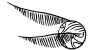
\includegraphics[scale=0.4]{boccino.png}
        \centering
\end{figure}

Harry Potter.

Doveva esserci qualcosa di strano a proposito di Harry Potter.

Era giovedì per tutti, in fin dei conti, e tuttavia questo genere di cose non sembravano accadere a nessun altro.

Erano le 18:21 di giovedì pomeriggio quando Harry Potter, uscendo sparato come una palla di cannone dalla tromba delle scale e accelerando al massimo della velocità, corse dritto contro Minerva McGonagall, che stava svoltando un angolo nel suo percorso verso l’ufficio del Preside.

Per fortuna nessuno si fece troppo male. Come era stato spiegato a Harry un po’ prima nel corso di quella stessa giornata — quando si stava rifiutando di avvicinarsi di nuovo minimamente a un manico di scopa — il Quidditch aveva bisogno di Bolidi di ferro pieno per avere una probabilità appena decente di ferire i giocatori, dal momento che i maghi tendevano a essere molto più resistenti agli urti dei Babbani.

Harry e la professoressa McGonagall finirono entrambi sul pavimento, e le pergamene che ella stava portando si sparsero per il corridoio.

Ci fu una terribile, terribile pausa.

«Harry Potter», prese fiato la professoressa McGonagall da là dove giaceva sul pavimento, proprio a fianco a Harry. La sua voce salì fino a divenire quasi un urlo. «Cosa stava facendo nell’ufficio del Preside?»

«Nulla!» squittì Harry.

«Stavate parlando del Professore di Difesa?»

«No! Silente mi ha convocato, e mi ha dato questa grossa roccia, e mi detto che era di mio padre e che dovrei portarmela sempre dietro!»

Ci fu un’altra terribile pausa.

«Capisco», disse la professoressa McGonagall, la sua voce un po’ più calma. Si alzò, si pulì, e fissò le pergamene sparse, che saltarono in una pila ordinata e corsero contro la parete del corridoio, come per nascondersi al suo sguardo. «Le mie simpatie, signor Potter, e mi scuso per aver dubitato di lei.»

«Professoressa McGonagall», Harry disse. La sua voce tremava. Si sollevò dal pavimento, si mise in piedi e guardò in su verso quel volto affidabile e sano di mente. «Professoressa McGonagall…»

«Sì, signor Potter?»

«Pensa che dovrei farlo?» Harry chiese a bassa voce. «Portare la roccia di mio padre ovunque con me?»

La professoressa McGonagall sospirò. «Questa è una faccenda tra lei e il Preside, temo.» Esitò. «Direi che ignorare completamente il Preside non è quasi mai saggio. Sono davvero dispiaciuta per il suo dilemma, signor Potter, e se ci fosse un modo in cui possa aiutarla con qualunque cosa lei decida di fare –»

«Uhm», Harry disse. «In realtà stavo pensando che una volta imparato come si fa, potrei Trasfigurare la roccia in un anello e infilarlo al dito. Se potesse insegnarmi come sostenere una Trasfigurazione –»

«È un bene che prima abbia chiesto a me», disse la professoressa McGonagall, il suo volto che stava diventando severo. «Se perdesse il controllo della Trasfigurazione, l’inversione le taglierebbe il dito e probabilmente le squarcerebbe la mano a metà. E alla sua età, anche un anello è un oggetto troppo grande per essere sostenuto indeterminatamente senza essere un severo drenaggio della sua magia. Ma posso farle forgiare un anello con un castone per un gioiello, un piccolo gioiello, a contatto con la sua pelle, e lei può far pratica sostenendo un oggetto sicuro, come una caramella morbida. Quando l’avrà sostenuto con successo, anche durante il sonno, per un mese intero, le permetterò di Trasfigurare, ah, la roccia di suo padre…» la voce della professoressa McGonagall si spense. «Il Preside le ha davvero –»

«Sì. Ah… uhm…»

La professoressa McGonagall sospirò. «È un po’ strano anche per lui.» Si chinò e raccolse la pila di pergamene. «Sono dispiaciuta per tutto ciò, signor Potter. Mi scuso di nuovo per aver diffidato di lei. Ma ora è il mio turno di vedere il Preside.»

«Ah… buona fortuna, credo. Ehm…»

«Grazie, signor Potter.»

«Uhm…»

La professoressa McGonagall si avvicinò al gargoyle, pronunciò impercettibilmente la parola d’accesso, ed entrò nelle scale a chiocciola ruotanti. Aveva cominciato a uscire fuori dal campo visivo, e il gargoyle aveva iniziato a tornare al proprio posto, quando –

«Professoressa McGonagall, il Preside ha dato fuoco a una gallina!»

«Che cos-»




% !TeX root = Harry.tex

\chapter{Gerarchie di dominanza}
\label{capitolo:18}

\emph{«Sembra il genere di cose che potrei fare, non è vero?»}

~\\
~\\


Era l’ora di colazione di venerdì mattina. Harry prese un altro grosso morso del suo pane tostato e poi cercò di ricordare al suo cervello che trangugiare la colazione non l’avrebbe portato prima nei sotterranei. Ad ogni modo, avevano un’intera ora di studio tra la colazione e l’inizio di Pozioni.

Ma, sotterranei! A Hogwarts! Nell’immaginazione di Harry stavano già nascendo immagini delle voragini, degli stretti ponti, dei sostegni per le torce e delle macchie di muschio luminescente. Ci sarebbero stati ratti? Ci sarebbero stati draghi?

«Harry Potter», disse una voce tranquilla dietro di lui.

Harry si guardò alle spalle e si trovò a contemplare Ernie Macmillan, elegantemente vestito con abiti dal bordo giallo e dall’espressione un po’ preoccupata.

«Neville ha pensato che avrei dovuto avvertirti», Ernie disse a voce bassa. «Credo che abbia ragione. Fai attenzione al Maestro di Pozioni nella nostra lezione di oggi. I Tassofrasso più grandi ci hanno detto che il professor Snape può essere davvero maligno con le persone che non gli piacciono, e non gli piace la maggior parte delle persone che non siano Serpeverde. Se gli dici qualcosa di impertinente… potrebbe finire davvero male per te, da quello che ho sentito. Tieni solo la testa bassa e non dargli alcun motivo per notarti.»

Ci fu una pausa mentre Harry elaborava quanto ascoltato, e poi sollevò le sopracciglia. (Harry avrebbe voluto alzare un solo sopracciglio, come Spock, ma non ne era mai stato capace.) «Grazie», disse Harry. «Potresti avermi appena risparmiato parecchi guai.»

Ernie annuì, e si voltò per tornare al tavolo dei Tassofrasso.

Harry riprese a mangiare il suo pane tostato.

Fu circa quattro morsi dopo che qualcuno disse «Scusami», e Harry si voltò per vedere un Corvonero più grande, dall’aspetto un po’ preoccupato –

Qualche tempo dopo, Harry stava finendo il suo terzo piatto di pancetta. (Aveva imparato a mangiare molto a colazione. Poteva sempre mangiare poco a pranzo, se non avesse finito per usare il Giratempo.) E c’era ancora un’altra voce dietro di lui che diceva «Harry?»

«Sì», disse Harry stancamente, «Cercherò di non attirare l’attenzione del professor Snape –»

«Oh, questo è impossibile», disse Fred.

«Assolutamente impossibile», disse George.

«Così abbiamo fatto cuocere una torta dagli elfi domestici», disse Fred.

«Abbiamo intenzione di metterci una candelina per ogni punto che perdi per Corvonero», disse George.

«E fare una festa per te al tavolo dei Grifondoro durante il pranzo», disse Fred.

«Ci auguriamo che ti tiri su il morale, dopo», concluse George.

Harry inghiottì il suo ultimo boccone di pancetta e si voltò. «Va bene», disse Harry. «Non avevo intenzione di chiederlo, dopo il professor Binns, davvero non volevo, ma se il professor Snape è così terribile, perché non è stato licenziato?»

«Licenziato?» disse Fred.

«Vuoi dire, mandato via?» disse George.

«Sì», rispose Harry. «È quello che si fa con i cattivi maestri. Li si licenzia. Poi si ingaggia un insegnante migliore al loro posto. Non avete sindacati o contratti a vita qui, giusto?»

Fred e George erano accigliati più o meno nello stesso modo in cui lo sarebbero stati gli anziani di una tribù di cacciatori-raccoglitori se avessero provato a spiegare loro il calcolo infinitesimale.

«Non lo so», disse Fred dopo un po’. «Non ci avevo mai pensato.»

«Nemmeno io», disse George.

«Sì», disse Harry, «me lo dicono spesso. Ci vediamo a pranzo, ragazzi, e non prendetevela con me se non ci saranno candeline su quella torta.»

Fred e George scoppiarono a ridere entrambi, come se Harry avesse detto qualcosa di divertente, gli rivolsero un inchino e si diressero verso Grifondoro.

Harry si girò di nuovo verso il tavolo della colazione e afferrò un pasticcino. Il suo stomaco era già pieno, ma aveva la sensazione che quella mattina avrebbe utilizzato molte calorie.

Mentre mangiava il suo pasticcino, Harry pensò al peggior insegnante che avesse conosciuto fino a quel momento, il professor Binns di Storia. Il professor Binns era un fantasma. Da quello che Hermione aveva detto dei fantasmi, non sembrava probabile che fossero pienamente consapevoli di sé. Non c’erano state scoperte famose fatte da fantasmi, o anche solo un lavoro originale, non importa chi fossero stati in vita. I fantasmi tendevano ad avere difficoltà a ricordare il secolo attuale. Hermione aveva detto che erano come ritratti fortuiti, impressi nella materia circostante dalla scarica di energia psichica che aveva accompagnato la morte improvvisa di un mago.

Harry aveva incontrato alcuni insegnanti stupidi durante le sue incursioni abortite nella normale istruzione babbana — suo padre era stato molto più esigente quando si era trattato di selezionare studenti universitari come precettori, ovviamente — ma il corso di storia era stato la prima volta che aveva incontrato un insegnante che letteralmente non era senziente.

E si vedeva, anche. Harry aveva rinunciato dopo cinque minuti e iniziato a leggere un libro di testo. Quando era stato chiaro che il «professor Binns» non avrebbe obiettato, Harry aveva messo la mano nella borsa e preso i tappi per le orecchie.

I fantasmi non prendevano stipendio? Era per questo? O era letteralmente impossibile licenziare qualcuno a Hogwarts anche se era morto?

Ora pareva che il professor Snape si stesse comportando in maniera assolutamente tremenda con tutti coloro che non fossero Serpeverde e non era neppure venuto in mente a qualcuno di rescindere il suo contratto.

E il Preside aveva dato fuoco a una gallina.

«Scusami», disse una voce preoccupata da dietro di lui.

«Giuro», disse Harry senza girarsi, «che questo posto è più brutto di circa l’otto e mezzo percento di quanto papà dica sia Oxford.»

\begin{figure}[h!]
        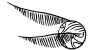
\includegraphics[scale=0.4]{boccino.png}
        \centering
\end{figure}

Harry pestava i piedi lungo i corridoi di pietra, apparentemente offeso, infastidito, e infuriato allo stesso tempo.

«Sotterranei!» sibilò Harry. «Sotterranei! Questi non sono sotterranei! Questa è una cantina! Una cantina!»

Alcune ragazze Corvonero lo guardarono come se fosse strano. I ragazzi erano tutti abituati a lui, ormai.

Sembrava che il livello in cui si trovava l’aula di Pozioni fosse detto dei «sotterranei» solo perché era sottoterra e un po’ più freddo del corpo principale del castello.

A Hogwarts! A Hogwarts! Harry aveva atteso tutta la vita e ora stava ancora aspettando e se c’era qualunque posto sulla faccia della Terra che avesse sotterranei decenti sarebbe dovuto essere Hogwarts! Harry doveva forse costruire il proprio castello se voleva vedere un po’ di abisso senza fondo?

Poco dopo arrivarono all’aula di Pozioni vera e propria e Harry si allietò considerevolmente.

L’aula di Pozioni conservava strane creature, galleggianti in enormi vasi sugli scaffali che coprivano ogni centimetro di muro tra gli armadi. Harry era andato abbastanza avanti nelle sue letture da poter realmente identificare alcune delle creature, come il Zabriskan Fontema. Sebbene il ragno di cinquanta centimetri sembrasse un’Acromantula, era troppo piccolo per esserne uno. Aveva provato a chiedere a Hermione, ma non sembrava molto interessata a guardare neppure vicino a dove stava indicando.

Harry stava osservando una grande palla di polvere con occhi e piedi quando l’assassino sfrecciò nella stanza.

Questo fu il primo pensiero che attraversò la mente di Harry quando vide il professor Severus Snape. C’era qualcosa di silenzioso e mortale nel modo in cui l’uomo si mosse tra i banchi dei bambini. I suoi abiti erano sciatti, i capelli unti e macchiati. Qualcosa in lui ricordava Lucius, anche se i due non si assomigliavano neppure lontanamente, e si aveva l’impressione che dove Lucius ti avrebbe ucciso con eleganza impeccabile, quest’uomo ti avrebbe semplicemente ucciso.

«Sedetevi», disse il professor Severus Snape. «Ora».

Harry e pochi altri bambini che erano stati in piedi a chiacchierare tra di loro scattarono verso i banchi. Harry aveva pensato di finire accanto a Hermione, ma in qualche modo si trovò seduto nel più vicino banco vuoto accanto a Justin Finch-Fletchley (era una Sessione doppia, Corvonero e Tassofrasso), cosa che lo poneva due banchi a sinistra di Hermione.

Severus si sedette dietro la cattedra, e senza la minima introduzione, disse «Hannah Abbott.»

«Eccomi», disse Hannah in una voce piuttosto tremante.

«Susan Bones.»

«Presente.»

E andò avanti così, nessuno che osava dire una parola fuori posto, finché:

«Ah, sì. Harry Potter. La nostra nuova… celebrità.»

«La celebrità è presente, signore.»

Metà della classe trasalì, e alcuni dei più intelligenti improvvisamente sembrarono voler correre fuori dalla porta a lezione ancora in corso.

Severus sorrise come in anticipazione e chiamò il successivo nome sulla sua lista.

Harry fece un sospiro mentale. Tutto era successo troppo velocemente perché potesse fare qualcosa a riguardo. Oh, bene. Chiaramente quest’uomo non lo aveva già in simpatia, quale che fosse il motivo. E pensandoci, molto meglio che questo professore di Pozioni se la prendesse con lui piuttosto che, diciamo, con Neville e Hermione. Harry era molto più bravo a difendersi. Sì, probabilmente tutto sarebbe andato per il meglio.

Quando l’appello fu terminato, Severus fece passare il suo sguardo sulla classe al completo. I suoi occhi erano vuoti come un cielo notturno senza stelle.

«Siete qui», disse Severus con una voce sommessa che gli studenti sul retro si sforzarono di udire, «per imparare la sottile scienza e l’esatta arte del preparare pozioni. Poiché qui c’è poco dello sciocco sventolar di bacchette, molti di voi difficilmente crederanno che questa sia magia. Non mi aspetto che comprendiate realmente la bellezza del calderone che ribolle dolcemente con i suoi vapori scintillanti, il delicato potere dei liquidi che si insinuano nelle vene umane», questo detto in un tono piuttosto carezzevole e compiaciuto, «stregando la mente e irretendo i sensi», tutto stava decisamente diventando sempre più inquietante e angosciante. «Io posso insegnarvi come imbottigliare la fama, fermentare la gloria, persino spillare la morte — se non foste un grande branco di stupidi come quelli cui normalmente insegno.»

In qualche modo Severus sembrò notare lo scetticismo dipinto sul volto di di Harry, o quanto meno i suoi occhi saltarono improvvisamente verso il posto dove si trovava seduto Harry.

«Potter!» disse bruscamente il Professore di Pozioni. «Che cosa ottengo se aggiungo radice di asfodelo in polvere in un infuso di assenzio?»

Harry sbatté le palpebre. «Era in Filtri magici e pozioni?» disse. «Ho appena finito di leggerlo, e non mi ricordo niente che usasse l’assenzio –»

La mano di Hermione si alzò e Harry le lanciò un’occhiataccia che gliela fece sollevare ancora più alto.

«Tsk, tsk», fece Severus. «La fama, chiaramente, non è tutto.»

«Davvero?» disse Harry. «Ma ci ha appena detto che ci insegnerà a imbottigliare la fama. Dica, come funziona esattamente? La si beve e ci si trasforma in una celebrità?»

Tre quarti della classe sussultarono.

La mano di Hermione stava scendendo lentamente verso il basso. Beh, non era una sorpresa. Poteva essere la sua rivale, ma non era il tipo di ragazza che sarebbe stata al gioco dopo che fosse diventato chiaro che il professore stava deliberatamente cercando di umiliarlo.

Harry stava tentando con forza di mantenere il controllo del suo temperamento. La prima risposta che aveva attraversato la sua mente era stata ‘Abracadabra’.

«Proviamo di nuovo», disse Severus. «Potter, dove cercheresti se ti avessi detto di trovarmi un bezoario?»

«Neanche questo è nel libro di testo», disse Harry, «ma in un libro babbano ho letto che un trichinobezoario è una massa di peli solidificati trovata in uno stomaco umano, e i Babbani credevano che fosse in grado di curare qualsiasi veleno –»

«Sbagliato», disse Severus. «Un bezoario si trova nello stomaco di una capra, non è fatto di capelli, ed è in grado di curare la maggior parte dei veleni, ma non tutti.»

«Non ho detto che sarebbe stato in grado di farlo, ho detto che era quello che ho letto in un libro babbano –»

«Qui nessuno è interessato ai suoi patetici libri babbani. Ultimo tentativo. Qual è la differenza, Potter, tra lo Strozzalupo e il Risigallo?»

Quella fu la goccia che fece traboccare il vaso.

«Sa», disse Harry gelidamente, «in uno dei miei libri babbani piuttosto affascinanti, si descrive uno studio in cui delle persone riuscivano a farsi passare per molto intelligenti ponendo domande su fatti qualunque di cui solo loro erano a conoscenza. A quanto pare gli osservatori notavano solo che chi faceva le domande sapeva le risposte e chi le riceveva no, e non riuscivano ad adattare il loro giudizio all’iniquità dello schema sottostante. Quindi, professore, è in grado di dirmi quanti elettroni ci sono nell’orbitale più esterno di un atomo di carbonio?»

Il sorriso di Severo si allargò. «Quattro», disse. «È un fatto inutile che nessuno dovrebbe preoccuparsi di mettere per iscritto, comunque. E per tua informazione, Potter, asfodelo e assenzio fanno una pozione soporifera così potente che è nota come la Bevanda della Morte Vivente. Per quanto riguarda lo Strozzalupo e il Risigallo, sono la stessa pianta, anche nota col nome di Aconito, come avresti saputo se avessi letto Mille erbe e funghi magici. Pensavi di non aver bisogno di aprire il libro prima di venire qui, eh, Potter? Tutti gli altri dovrebbero copiare quanto detto, in modo da non essere così ignoranti come lui.» Severus fece una pausa, sembrando alquanto soddisfatto di sé stesso. «E questo varrà… cinque punti? No, facciamo dieci punti tondi da Corvonero per insolenza.»

Hermione rantolò, insieme a diversi altri.

«Professor Severus Snape», Harry profferì. «Non so cosa io possa aver fatto per meritare la sua ostilità. Se ha qualche problema con me di cui non sono al corrente, suggerisco che noi –»

«Stia zitto, Potter. Altri dieci punti da Corvonero. Voi altri, aprite i vostri libri a pagina 3.»

C’era solamente una sensazione leggera, solamente una sensazione molto debole di bruciore nella parte posteriore della gola di Harry, e nessuna umidità nei suoi occhi. Se piangere non era un strategia efficace per distruggere questo Professore di Pozioni, allora era inutile piangere.

Lentamente, Harry raddrizzò la schiena. Tutto il suo sangue sembrava essere defluito e sostituito da azoto liquido. Sapeva che aveva provato a controllare il suo temperamento, ma non sembrava in grado di ricordare perché.

«Harry», sussurrò freneticamente Hermione due banchi più in là, «fermati, per favore, è tutto a posto, non li conteremo –»

«Parla durante la lezione, Granger? Tre –»

«Dunque», disse una voce più fredda di zero gradi Kelvin, «cosa si deve fare per presentare un reclamo formale contro un professore molesto? Bisogna parlare con la Vicepreside, scrivere una lettera al Consiglio Direttivo… le dispiacerebbe spiegare come funziona?»

La classe era completamente paralizzata.

«Detenzione per un mese, Potter», disse Severus, sorridendo ancor più largamente.

«Mi rifiuto di riconoscere la sua autorità di insegnante e non sconterò alcuna detenzione data da lei.»

Le persone smisero di respirare.

Il sorriso di Severus svanì. «Allora sarai –» la sua voce si interruppe bruscamente.

«Espulso, stava per dire?» Harry, d’altra parte, stava ora accennando un sorriso. «Ma poi è sembrato dubitare della sua capacità di attuare la sua minaccia, o temerne le conseguenze. Io, al contrario, non ho dubbi né timori alla prospettiva di trovare un’altra scuola con professori meno molesti. O forse dovrei pagare dei precettori privati, come sono solito fare, e ricevere un’educazione che sia alla mia piena velocità di apprendimento. Ho abbastanza denaro nel mio deposito. Qualcosa a proposito di taglie su di un Signore Oscuro che ho sconfitto. Ma ci sono insegnanti a Hogwarts che mi piacciono abbastanza, quindi credo che sarebbe più semplice se trovassi il modo di sbarazzarmi di lei, invece.»

«Sbarazzarsi di me?» disse Severus, anch’egli con un accenno di sorriso, ora. «Che idea divertente. Come pensa di farlo, Potter?»

«Mi par di capire che ci sia stato un certo numero di lamentele contro di lei da parte degli studenti e dei loro genitori», una congettura, ma piuttosto sicura, «cosa che lascia solo la questione del perché non se ne sia già andato. Forse le finanze di Hogwarts non possono permettersi un vero Professore di Pozioni? Potrei dare il mio contributo. Sono certo che troverebbero un professore di ben altro livello se offrissero il doppio del suo salario corrente.»

Due poli di ghiaccio irraggiavano un inverno congelante attraverso l’aula.

«Scoprirà», Severus disse mollemente, «che il Consiglio Direttivo non è minimamente interessato alla sua offerta.»

«Lucius…» disse Harry. «Ecco perché lei è ancora qui. Forse dovrei fare una chiacchierata con Lucius a riguardo. Credo che desideri incontrarmi. Mi chiedo se ho qualcosa che lo interessa.»

Hermione scosse la testa freneticamente. Harry lo notò con la coda dell’occhio, ma la sua attenzione era tutta su Severus.

«Lei è un ragazzo molto sciocco», disse Severus. Non sorrideva affatto, adesso. «Non ha niente che Lucius desideri più della mia amicizia. E se l’avesse, ho altri alleati.» La sua voce si fece dura. «E trovo sempre più improbabile che lei non sia stato Smistato in Serpeverde. Com’è riuscito a rimanere fuori dalla mia Casa? Ah, sì, perché il Cappello Smistatore ha detto che stava scherzando. Per la prima volta nella storia. Di cosa stava parlando realmente col Cappello Smistatore, Potter? Possiede qualcosa che voleva?»

Harry fissò lo sguardo freddo di Severus e ricordò che il Cappello Smistatore lo aveva avvertito di non incrociare lo sguardo di chiunque mentre stava pensando a — Harry abbassò lo sguardo sulla scrivania di Severus.

«Sembra stranamente riluttante a guardarmi negli occhi, Potter!»

Una scossa di comprensione improvvisa — «Quindi è stato contro di lei che il Cappello Smistatore mi ha messo in guardia!»

«Cosa?» disse la voce di Severus, che sembrò sinceramente sorpreso, anche se naturalmente Harry non lo guardò in faccia.

Harry si alzò dal suo banco.

«Si segga, Potter», disse una voce arrabbiata da qualche luogo in cui non stava guardando.

Harry lo ignorò, e guardò l’aula. «Non ho alcuna intenzione di lasciare che un insegnante non professionale rovini la mia permanenza a Hogwarts», disse Harry mortalmente calmo. «Penso che mi congederò da questo corso, e o assumerò un tutore per insegnarmi Pozioni mentre sono qui, o se il Consiglio è davvero sotto controllo, studierò durante l’estate. Se qualcuno di voi decidesse che non gli interessa essere vittima del bullismo di quest’uomo, le mie sessioni saranno aperte anche a lui.»

«Si segga, Potter!»

Harry attraversò la stanza e afferrò la maniglia della porta.

Non girò.

Harry si voltò lentamente, e colse l’immagine di Severus che sorrideva malignamente prima di ricordarsi di guardare altrove.

«Apra questa porta.»

«No», disse Severus.

«Mi sta facendo sentire minacciato», disse una voce così gelida che non sembrava affatto quella di Harry, «e questo è un errore.»

La voce di Severus rise. «Cosa intende fare, ragazzino?»

Harry misurò sei lunghi passi dalla porta, finché non fu in piedi vicino all’ultima fila di banchi.

Poi si mise perfettamente eretto e alzò la mano destra in un unico e terribile movimento, le dita pronte a schioccare.

Neville urlò e si tuffò sotto il banco. Altri bambini si ritrassero o alzarono istintivamente le braccia per proteggersi.

«Harry no!» strillò Hermione. «Qualunque cosa avessi intenzione di fargli, non farlo!»

«Siete diventati tutti pazzi?» abbaiò la voce di Severus.

Lentamente, Harry abbassò la mano. «Non avevo intenzione di fargli del male, Hermione», disse Harry, la sua voce un po’ più bassa. «Stavo per far saltare in aria la porta.»

Anche se ora che Harry ci stava pensando, era proibito Trasfigurare oggetti da bruciare, il che significava che andare indietro nel tempo e convincere Fred o George a trasfigurare una quantità precisamente misurata di esplosivi sarebbe potuta non essere realmente un buona idea…

«Silencio», disse la voce di Severus.

Harry cercò di dire «Che cosa?» e scoprì che non gli usciva alcun suono.

«Questa è diventata una farsa. Credo che le sia stato permesso di mettersi sufficientemente nei guai per un solo giorno, Potter. Lei è lo studente più molesto e indisciplinato che abbia mai incontrato, e non ricordo quanti punti Corvonero abbia in questo momento, ma sono sicuro di poterli a spazzare via tutti. Dieci punti da Corvonero. Dieci punti da Corvonero. Dieci punti da Corvonero! Cinquanta punti da Corvonero! Ora si segga e osservi il resto della classe fare lezione!»

Harry mise la mano in tasca e cercò di dire ‘pennarello’, ma ovviamente nessuna parola uscì fuori. Per un breve momento, questo lo fermò; poi gli venne in mente di formare la sequenza p-e-n-n-a-r-e-l-l-o con i movimenti delle dita, e questo funzionò. b-l-o-c-c-o ed ebbe il blocco di carta. Harry si diresse a un banco vuoto, non quello dove era originariamente seduto, e scarabocchiò un breve messaggio. Strappò quel foglio di carta, mise via il pennarello e il blocco in una tasca della sua veste per un accesso più rapido, e alzò il suo messaggio, non verso Severus, ma verso il resto della classe.

me ne vado

qualcun altro ha

bisogno di uscire?

«Lei è folle, Potter», disse Severus con freddo disprezzo.

A parte quello, nessuno parlò.

Harry indirizzò un ironico inchino verso la cattedra, si avvicinò alla parete, e con un unico movimento fluido spalancò la porta di uno stanzino, ci entrò e sbatté la porta dietro di sé.

Ci fu il suono ovattato di qualcuno che schioccava le dita, e poi più nulla.

In classe, gli studenti si guardarono l’un l’altro perplessi e impauriti.

Il volto del Maestro di Pozioni era ora completamente infuriato. Attraversò la stanza a grandi passi terribili e spalancò la porta dello stanzino.

Lo stanzino era vuoto.

\begin{figure}[h!]
        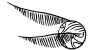
\includegraphics[scale=0.4]{boccino.png}
        \centering
\end{figure}

Un’ora prima, Harry si mise in ascolto all’interno dello stanzino chiuso. Non c’era alcun suono all’esterno, e neppure alcun motivo di rischiare.

m-a-n-t-e-l-l-o, formarono le sue dita.

Una volta resosi invisibile, con molta attenzione e circospezione aprì la porta dello stanzino e sbirciò fuori. In classe non sembrava esserci nessuno.

La porta non era chiusa a chiave.

Fu quando Harry si trovò fuori da quel luogo pericoloso e dentro il corridoio, sicuro e invisibile, che un po’ di quella rabbia sparì e si rese conto di quello che aveva appena fatto.

Quello che aveva appena fatto.

Il volto invisibile di Harry si paralizzò per l’orrore assoluto.

Si era inimicato un insegnante tre ordini di grandezza al di là di qualsiasi cosa avesse mai gestito prima. Aveva minacciato di andarsene da Hogwarts e avrebbe potuto dover dar seguito alla minaccia. Aveva perso tutti i punti che Corvonero aveva e poi aveva usato il Giratempo…

La sua immaginazione gli mostrò i suoi genitori che gli urlavano contro dopo che era stato espulso, e la professoressa McGonagall delusa, ed era troppo doloroso e non poteva sopportarlo e non riusciva a pensare a un modo per salvarsi –

Il pensiero che Harry si concesse era che se arrabbiarsi lo aveva infilato in tutti quei guai, allora forse quando fosse stato nuovamente infuriato avrebbe trovato una via d’uscita, le cose sembravano in qualche modo più chiare quando era arrabbiato.

E il pensiero che Harry non si concesse era che non riusciva proprio ad affrontare questa prospettiva, se non era arrabbiato.

Così ricacciò tutti i suoi pensieri e ricordò la bruciante umiliazione –

Tsk, tsk. La fama, chiaramente, non è tutto.

Dieci punti da Corvonero per insolenza.

Il freddo calmante ripulì le sue vene come la risacca di un’onda riflessa da un ostacolo, e Harry si permise di espirare.

Va bene. Torna ad essere sano di mente, ora.

Si sentiva veramente un po’ deluso dal sé stesso non arrabbiato per essere crollato così e aver voluto solo uscire dai guai. Il professor Severus Snape era un problema di tutti. L’Harry-Normale l’aveva dimenticato e aveva desiderato un modo per proteggere sé stesso. E chi se ne frega di tutte le altre vittime? La questione non era come proteggere sé stesso, la questione era come distruggere questo Professore di Pozioni.

Quindi questo è il mio lato oscuro, vero? C’è un po’ di pregiudizio in questo termine, il mio lato illuminato sembra più egoista e codardo, per non dire confuso e in preda al panico.

E ora che stava pensando chiaramente, fu parimenti chiaro cosa fare dopo. Aveva già dato a sé stesso un’ora in più per prepararsi, e avrebbe potuto prendersi fino a cinque ore ulteriori, se necessario…

\begin{figure}[h!]
        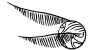
\includegraphics[scale=0.4]{boccino.png}
        \centering
\end{figure}

Minerva McGonagall attendeva nell’ufficio del Preside.

Silente sedeva nel suo trono imbottito dietro la scrivania, vestito con quattro strati di vesti formali color lavanda. Minerva sedeva su una sedia di fronte a lui, dall’altro lato Severus in un’altra sedia. Di fronte a loro tre c’era uno sgabello di legno vuoto.

Stavano aspettando Harry Potter.

Harry, Minerva pensò disperata, avevi promesso che non avresti morso alcun insegnante!

E nella sua mente riuscì a visualizzare molto chiaramente la replica, il volto arrabbiato di Harry e la sua risposta indignata: ho detto che non avrei morso chiunque non mi avesse morso per primo!

Qualcuno bussò alla porta.

«Avanti!» chiamò Silente.

La porta si aprì, e Harry Potter entrò. Minerva si lasciò quasi scappare un forte gemito. Il ragazzo sembrava glaciale, calmo, e assolutamente nel pieno controllo di sé stesso.

«Buon gior-» la voce di Harry si interruppe improvvisamente. La sua bocca rimase aperta.

Minerva seguì lo sguardo di Harry, e vide che stava fissando Fawkes, appollaiato sul trespolo dorato. Fawkes sventolò le sue brillanti ali rosso-dorate come il tremolio di una fiamma, e abbassò la testa in un cenno misurato al ragazzo.

Harry si voltò a guardare Silente.

Silente gli fece l’occhiolino.

Minerva percepì che si era persa qualcosa.

Un’incertezza improvvisa attraversò il volto di Harry. La sua freddezza vacillò. Nei suoi occhi si mostrò la paura, poi la rabbia, e poi il ragazzo fu nuovamente calmo.

Un brivido scese lungo la schiena di Minerva. C’era qualcosa che non andava.

«Accomodati» disse Silente. Il suo volto era di nuovo serio.

Harry si sedette.

«Allora, Harry» disse Silente. «Ho sentito una relazione di questa giornata da parte del professor Snape. Ti andrebbe di dirmi cosa è successo con parole tue?»

Harry indirizzò un’occhiata sprezzante a Severus. «Non è complicato», disse il ragazzo, sorridendo appena. «Ha provato a comportarsi da bullo con me nello stesso modo in cui molesta tutti quelli qui a scuola che non appartengono a Serpeverde dal giorno che Lucius ve l’ha imposto. Per quanto riguarda gli altri dettagli, chiedo una conversazione privata con lei su questo argomento. Da uno studente che sta denunciando il comportamento abusivo di un professore difficilmente ci si può aspettare che parli con franchezza di fronte a quello stesso professore, dopo tutto.»

Questa volta Minerva non poté impedirsi di gemere forte.

Severus, semplicemente, rise.

E il volto del Preside divenne severo. «Signor Potter», disse, «non si parla di un professore di Hogwarts in questi termini. Ho paura che lei stia agendo sulla base di un terribile equivoco. Il professor Severus Snape ha la mia piena fiducia, ed è al servizio di Hogwarts dietro mia richiesta, non di Lucius Malfoy.»

Ci fu silenzio per alcuni momenti.

Quando il ragazzo parlò nuovamente, la sua voce era di ghiaccio. «Mi sono perso qualcosa?»

«Un certo numero di cose, signor Potter», disse il Preside. «Dovrebbe capire, per iniziare, che lo scopo di questo incontro è discutere come punirla per gli eventi di questa mattina.»

«Quest’uomo ha terrorizzato la sua scuola per anni. Ho parlato agli studenti e raccolto testimonianze per essere certo che ce ne fossero abbastanza per una campagna giornalistica, allo scopo di unire i genitori contro di lui. Alcuni degli studenti più giovani piangevano mentre me ne parlavano. Io ho quasi pianto ascoltandoli! Lei ha permesso a questo prevaricatore di agire liberamente? Ha fatto questo ai suoi studenti? Perché?»

Minerva deglutì un groppo in gola. Aveva — pensato la stessa cosa, talvolta, ma per qualche ragione non era mai del tutto –

«Signor Potter», disse il Preside, la sua voce ora severa, «questo incontro non riguarda il professor Snape. Riguarda lei e il suo disprezzo per la disciplina scolastica. Il professor Snape ha suggerito, e io ho concordato, che tre mesi interi di detenzione saranno appropriati –»

«Respinto», disse Harry gelidamente.

Minerva era senza parole.

«Questa non è una richiesta, signor Potter», disse il Preside. Tutta la forza dello sguardo del mago fu concentrata sul ragazzo. «Questa è la sua punizio-»

«Lei mi spiegherà perché ha permesso a quest’uomo di fare del male ai bambini affidati alle sue cure, e se la sua spiegazione non sarà sufficiente, allora inizierò la mia campagna giornalistica con lei come bersaglio.»

Il corpo di Minerva ondeggiò per la forza di quel colpo, per la pura lesa maestà.

Anche Severus sembrò scioccato.

«Questo, Harry, sarebbe estremamente imprudente», disse Silente lentamente. «Io sono il pezzo principale che sulla scacchiera si oppone a Lucius. Se facessi una cosa del genere lo rafforzeresti notevolmente, e non pensavo che fosse questo lo schieramento che avevi scelto.»

Il ragazzo rimase fermo per un lungo momento.

«Questa conversazione diventa privata», disse Harry. La sua mano scattò in direzione di Severus. «Lo mandi via.»

Silente scosse la testa. «Harry, non ti ho detto che Severus Snape ha la mia piena fiducia?»

Il viso del ragazzo mostrò lo sconcerto. «Il bullismo di quest’uomo la rende vulnerabile! Non sono l’unico che potrebbe dare inizio a una campagna giornalistica contro di lei! Questo è folle! Perché sta agendo così?»

Silente sospirò. «Mi dispiace, Harry. Ha a che fare con cose che non sei, in questo momento, pronto a sentire.»

Il ragazzo fissò Silente. Poi si voltò a guardare Severus. Poi di nuovo Silente.

«Questa è follia», disse il ragazzo lentamente. «Lei non l’ha tenuto a freno perché pensa che lui sia parte dello schema. Che Hogwarts abbia bisogno di un Maestro di Pozioni cattivo per essere una vera e propria scuola di magia, così come ha bisogno di un fantasma per insegnare Storia.»

«Sembra il genere di cose che potrei fare, non è vero?» disse Silente, sorridendo.

«Inaccettabile», rispose Harry in tono piatto. Il suo sguardo era ormai freddo e buio. «Non tollererò bullismo o abusi. Avevo considerato molti modi possibili di affrontare questo problema, ma la farò semplice. O se ne va quest’uomo, o lo faccio io.»

Minerva rimase nuovamente a bocca aperta. Qualcosa di strano balenò negli occhi di Severus.

Ora anche lo sguardo di Silente stava diventando freddo. «L’espulsione, signor Potter, è la minaccia finale che può essere usata contro uno studente. Non viene abitualmente utilizzata dagli studenti come minaccia nei confronti del Preside. Questa è la migliore scuola di magia in tutto il mondo, e un’educazione qui non è un’opportunità data a tutti. Ha l’impressione che Hogwarts non possa andare avanti senza di lei?»

E Harry rimase seduto, un accenno di sorriso.

Un orrore improvviso balenò nella mente di Minerva. Sicuramente Harry non avrebbe –

«Lei dimentica», disse Harry, «che non è l’unico che può vedere gli schemi ricorrenti. Questa sta diventando una faccenda privata. Ora lo mandi –» Harry fece nuovamente un gesto verso Severus, e poi si fermò a metà frase e a metà gesto.

Minerva poté vederlo sul viso di Harry, il momento in cui si ricordò.

Dopo tutto era stata lei a dirglielo.

«Signor Potter», disse il Preside, «ancora una volta, Severus Snape ha la mia piena fiducia.»

«Gliel’ha detto», sussurrò il ragazzo. «Lei è completamente folle.»

Silente non reagì all’insulto. «Detto cosa?»

«Che il Signore Oscuro è vivo.»

«In nome di Merlino, di che cosa sta parlando, Potter?» esclamò Severus coi toni più puri dello stupore e dell’indignazione.

Harry lo guardò brevemente, con un sorriso cupo. «Oh, quindi è un Serpeverde, allora», disse Harry. «Stavo cominciando a dubitarne.»

E poi ci fu silenzio.

Infine Silente parlò. La sua voce era dolce. «Harry, di che cosa stai parlando?»

«Mi dispiace, Albus», sussurrò Minerva.

Severus e Silente si voltarono a guardarla.

«Non me l’ha detto la professoressa McGonagall», disse Harry con un tono sbrigativo e meno calmo di prima. «L’ho indovinato io. Gliel’ho detto, anche io posso vedere gli schemi ricorrenti. L’ho indovinato, e lei ha controllato la sua reazione proprio come ha fatto Severus. Ma la sua reazione è stata di un’ombra inferiore alla perfezione, e ho potuto capire che era controllata e non genuina.»

«E gli ho detto», disse Minerva, la voce un po’ tremante, «che tu e io, e Severus eravamo gli unici a saperlo.»

«Cosa che ha fatto come una concessione a me, per impedirmi di andarmene in giro a fare domande, come avevo minacciato di fare se non avesse parlato», disse Harry. Il ragazzo ridacchiò brevemente. «Avrei dovuto davvero prendere uno di voi e dirgli che mi aveva detto tutto, per vedere se gli sarebbe sfuggito qualcosa. Probabilmente non avrebbe funzionato, ma sarebbe valsa la pena provarci.» Il ragazzo sorrise di nuovo. «La minaccia è ancora valida e mi aspetto di essere informato pienamente prima o poi.»

Severus le stava indirizzando uno sguardo di disprezzo. Minerva alzò il mento e lo sopportò. Sapeva che se l’era meritato.

Silente si appoggiò al trono imbottito. I suoi occhi erano freddi come mai Minerva li aveva visti dal giorno in cui suo fratello era morto. «E tu minacci di abbandonarci a Voldemort, se non ci adeguassimo ai tuoi desideri.»

Il tono di Harry fu tagliente. «Sono spiacente di informarvi che non siete il centro dell’universo. Non sto minacciando di abbandonare la Gran Bretagna magica. Sto minacciando di abbandonare voi. Io non sono un piccolo e mite Frodo. Questa è la mia impresa e se volete farne parte dovrete giocare secondo le mie regole.»

Il volto di Silente era ancora freddo. «Sto cominciando a dubitare della sua adeguatezza come eroe, signor Potter.»

Lo sguardo che Harry restituì era altrettanto gelido. «Sto cominciando a dubitare della sua adeguatezza come mio Gandalf, signor Silente. Almeno Boromir fu un errore comprensibile. Cosa ci fa questo Nazgûl nella mia Compagnia?»

Minerva era completamente persa. Guardò Severus, per vedere se stava seguendo, e notò che aveva girato il suo volto lontano dal campo visivo di Harry e stava sorridendo.

«Suppongo», disse Silente lentamente, «che dal suo punto di vista si tratti di una domanda ragionevole. Allora, signor Potter, se il professor Snape la lasciasse in pace d’ora in poi, sarà questa l’ultima volta che la questione si pone, o la troverò qui ogni settimana con una nuova richiesta?»

«Lasciare in pace me?» Il tono di Harry era indignato. «Non sono la sua unica vittima e certo non la più vulnerabile! Avete dimenticato quanto siano indifesi i bambini? Quanto vengono feriti? D’ora in poi Severus tratterà ogni studente di Hogwarts con adeguata e professionale cortesia, oppure si troverà un altro Maestro di Pozioni, oppure un altro eroe!»

Silente cominciò a ridere. Una risata a piena gola, calda, divertita, come se Harry avesse appena fatto un numero comico di fronte a lui.

Minerva non osava muoversi. I suoi occhi tremarono e vide che Severus era ugualmente immobile.

Il volto di Harry divenne ancora più freddo. «Lei mi fraintende, Preside, se pensa che questo sia uno scherzo. Questa non è una richiesta. Questa è la sua punizione.»

«Signor Potter –» disse Minerva. Non sapeva nemmeno quello che stava per dire. Semplicemente non poteva ignorare quella risposta.

Harry fece un gesto per zittirla e continuò a parlare a Silente. «E se questo le sembra scortese», disse, la sua voce ora un po’ meno dura, «non è sembrato meno scortese quando lei l’ha detto a me. Non direbbe una cosa del genere a chiunque considerasse un vero essere umano invece di un bambino a lei subordinato, e la tratterò con la stessa cortesia con cui lei tratta me –»

«Oh, è vero, è proprio vero, questa è la mia punizione se mai ce ne sia stata una! È ovvio che sei qui a ricattarmi per salvare i tuoi compagni, non per salvare te stesso! Non riesco a immaginare perché ho pensato il contrario!» Ora Silente rideva ancora più fragorosamente. Batté il pugno sul tavolo tre volte.

Lo sguardo di Harry divenne incerto. Il suo viso si voltò verso Minerva, rivolgendosi a lei per la prima volta. «Mi scusi», disse Harry. La sua voce sembrò vacillare. «Ha bisogno di prendere le sue medicine o cosa?»

«Ah…» Minerva non aveva idea di cosa potesse rispondere.

«Bene», disse Silente. Si asciugò le lacrime che si erano formate nei suoi occhi. «Mi scusi. Mi dispiace per l’interruzione. La prego, continui con il ricatto.»

Harry aprì la bocca, poi la richiuse. Ora sembrava un po’ incerto. «Ah… deve anche smettere di leggere nelle menti degli studenti.»

«Minerva», disse Severus, la sua voce letale, «tu –»

«È stato il Cappello Smistatore ad avvertirmi», disse Harry.

«Cosa?»

«Non posso dire nient’altro. Ad ogni modo, penso sia tutto qui. Ho finito.»

Silenzio.

«E ora?» disse Minerva, quando divenne chiaro che nessun altro stava per dire qualcosa.

«E ora?» Silente le fece eco. «Beh, e ora l’eroe vince, ovviamente.»

«Cosa?» dissero Severus, Minerva, e Harry.

«Beh, certamente sembra che ci abbia stretti in un angolo», disse Silente, sorridendo felice. «Ma Hogwarts ha realmente bisogno di un Maestro di Pozioni cattivo, o non sarebbe una vera e propria scuola di magia, non credete? Quindi che ne pensi se il professor Snape sarà tremendo solo nei confronti degli studenti dal loro quinto anno e in poi?»

«Cosa?» dissero nuovamente tutti e tre.

«Se sono le vittime più vulnerabili che ti preoccupano. Forse hai ragione, Harry. Forse io ho dimenticato nel corso dei decenni che cosa vuol dire essere un bambino. Quindi cerchiamo un compromesso. Severus continuerà ad aggiudicare ingiustamente punti a Serpeverde e a imporre una disciplina lassista sulla sua Casa, e sarà terribile con gli studenti non appartenenti a Serpeverde dal loro quinto anno in poi. Con tutti gli altri sarà spaventoso, ma non molesto. Prometterà di leggere le menti solo quando la sicurezza di uno studente lo richiedesse. Hogwarts avrà il suo Maestro di Pozioni cattivo, e le vittime più vulnerabili, come dici tu, saranno al sicuro.»

Minerva McGonagall era scioccata più di quanto fosse mai stata in vita sua. Lanciò un’occhiata incerta a Severus, il cui volto era rimasto completamente neutro, come se non riuscisse a decidere che tipo di espressione avrebbe dovuto assumere.

«Presumo che sia accettabile», disse Harry. La sua voce suonò un po’ strana.

«Non puoi parlare sul serio», disse Severus, la sua voce inespressiva come il suo volto.

«Sono molto favorevole», disse lentamente Minerva. Era tanto favorevole che il suo cuore batteva all’impazzata sotto le sue vesti. «Ma cosa possiamo dire agli studenti? Non si saranno lamentati quando Severus è stato… terribile con tutti, ma –»

«Harry può dire agli altri studenti che ha scoperto un terribile segreto di Severus e ha esercitato un piccolo ricatto» disse Silente. «È vero, dopo tutto; ha scoperto che Severus stava leggendo le menti, e di certo ci ha ricattati.»

«Questa è follia!» esplose Severus.

«Bwah ah ah!» disse Silente.

«Ah…» disse Harry incerto. «E se qualcuno mi chiedesse perché quelli dal quinto anno in su sono rimasti fregati? Non li biasimerei se si arrabbiassero, e quella parte dell’accordo non è esattamente idea mia –»

«Racconta loro», rispose Silente, «che non sei stato tu a suggerire il compromesso, che era tutto ciò che hai potuto ottenere. E poi rifiutati di dire altro. Anche questo è vero. È una specie di arte, ci farai la mano con la pratica.»

Harry annuì lentamente. «E i punti che ha sottratto a Corvonero?»

«Non devono essere restituiti.»

Era stata Minerva a parlare.

Harry la guardò.

«Mi dispiace, signor Potter». Era dispiaciuta, ma doveva essere fatto. «Ci devono essere delle conseguenze per la sua cattiva condotta o questa scuola cadrà a pezzi.»

Harry scrollò le spalle. «Accettabile», disse senza emozione. «Ma in futuro Severus non colpirà i miei rapporti con la Casa sottraendomi punti, né sprecherà il mio tempo prezioso con detenzioni. Se ritenesse che il mio comportamento richieda una punizione, potrà comunicare le sue preoccupazioni alla professoressa McGonagall.»

«Harry», disse Minerva, «continuerai a restare soggetto alla disciplina scolastica, o sarai al di sopra della legge, come è stato Severus?»

Harry la guardò. Un certo calore toccò il suo sguardo, poco prima di essere represso. «Continuerò a essere uno studente ordinario per ogni membro del personale che non sia pazzo o cattivo, a condizione che non sia messo sotto pressione da altri che lo sono.» Harry guardò brevemente Severus, poi si voltò verso Silente. «Lasciate stare Minerva, e sarò un normale studente di Hogwarts in sua presenza. Nessun particolare privilegio o immunità.»

«Bellissimo», disse Silente sinceramente. «Parli come un vero eroe.»

«E inoltre», ella disse, «il signor Potter deve scusarsi pubblicamente per le sue azioni di oggi.»

Harry le rivolse un’altra occhiata. Questa era un po’ scettica.

«La disciplina della scuola è stata gravemente danneggiata dalle sue azioni, signor Potter», disse Minerva. «Deve essere ripristinata.»

«Penso, professoressa McGonagall, che lei sopravvaluti considerevolmente l’importanza di ciò che chiama disciplina scolastica, rispetto ad avere il corso di Storia insegnato da un insegnante vivente o a non torturare i vostri studenti. Il mantenimento dello status quo gerarchico e l’applicazione delle sue regole sembrano sempre molto più saggi, morali e importanti quando si è in alto e si fa rispettare tale applicazione di quando si è in basso, e posso citare degli studi in tal senso, se necessario. Potrei andare avanti per ore su questo punto, ma finirò qui.»

Minerva scosse la testa. «Signor Potter, lei sottovaluta l’importanza della disciplina perché lei non ne ha bisogno –» Fece una pausa. Non era venuto fuori in maniera giusta, e Severus, Silente e persino Harry le stavano rivolgendo delle strane occhiate. «Per imparare, intendo. Non tutti i bambini sono in grado di imparare in assenza di autorità. E saranno gli altri bambini a essere danneggiati, signor Potter, se crederanno che il suo sia un esempio da seguire.»

Le labbra di Harry s’incurvarono in un sorriso contorto. «La prima e l’ultima risorsa è la verità. La verità è che non mi sarei dovuto arrabbiare, che non avrei dovuto disturbare la lezione, che non avrei dovuto fare ciò che ho fatto e che ho dato un cattivo esempio a tutti. La verità è anche che Severus Snape si è comportato in modo indegno di un professore di Hogwarts, e che d’ora in poi starà molto più attento a non ferire i sentimenti degli studenti dal quarto anno in giù. Entrambi potremmo alzarci e dire la verità. Potrei accettare questo.»

«Nei tuoi sogni, Potter!» esclamò Severus.

«Dopotutto», disse Harry, sorridendo cupamente, «se gli studenti vedessero che le regole valgono per tutti… anche per i professori, non solo per i poveri studenti indifesi che non ricevono altro che sofferenza dal sistema… beh, gli effetti positivi sulla disciplina scolastica sarebbero straordinari.»

Ci fu una breve pausa, e poi Silente ridacchiò. «Minerva sta pensando che hai più ragione di quanto avresti il diritto di avere.»

Lo sguardo di Harry corse via da Silente, giù verso il pavimento. «Lei sta leggendo la sua mente?»

«Il buon senso è spesso confuso con la Legilimanzia», disse Silente. «Discuterò di questo con Severus, e non ti sarà chiesta alcuna scusa a meno che lui non si scusi allo stesso modo. E ora dichiaro chiusa questa faccenda, almeno fino all’ora di pranzo.» Fece una pausa. «Sebbene, Harry, temo che Minerva desiderasse parlarti di un ulteriore affare. E questo non è il risultato di alcuna pressione da parte mia. Minerva, ti dispiace?»

Minerva si alzò dalla sedia e quasi cadde. C’era troppa adrenalina nel suo sangue, il suo cuore stava battendo troppo velocemente.

«Fawkes», disse Silente, «accompagnala, per favore.»

«Io non –» ella iniziò a dire.

Silente la guardò, ed ella si azzittì.

La fenice si librò per la stanza come una lingua di fuoco che scatta d’improvviso, e atterrò sulla sua spalla. Ella sentì il calore attraverso le proprie vesti, espandersi attraverso tutto il suo corpo.

«La prego di seguirmi, signor Potter», disse ora fermamente, e uscirono dalla porta.

\begin{figure}[h!]
        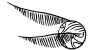
\includegraphics[scale=0.4]{boccino.png}
        \centering
\end{figure}

Erano in piedi sulle scale ruotanti, scendendo in silenzio.

Minerva non sapeva cosa dire. Non conosceva la persona che stava al suo fianco.

E Fawkes iniziò il suo canto.

Era tenero, e soffuso, come avrebbe suonato un caminetto se avesse avuto una melodia, e inondò la mente di Minerva, alleviando, calmando, lenendo ciò che toccava…

«Che cos’è quello?» sussurrò Harry al suo fianco. La sua voce era variabile, tremolante, dal tono cangiante.

«La canzone della fenice», rispose Minerva, non realmente cosciente di ciò che diceva, la sua attenzione era tutta per quella musica strana, calma. «Anch’essa guarisce.»

Harry rivolse il volto dall’altra parte, ma ella fu in grado di cogliere un’occhiata di agonia.

La discesa sembrò richiedere un tempo molto lungo, o forse fu solo che la musica sembrò richiedere un tempo molto lungo, e quando uscirono dal varco lasciato dal gargoyle, stava fermamente reggendo la mano di Harry tra le proprie.

Quando il gargoyle tornò al suo posto, Fawkes lasciò la sua spalla, e discese repentinamente per librarsi di fronte a Harry.

Harry fissò Fawkes come qualcuno ipnotizzato dalla luce cangiante di un incendio.

«Cosa devo fare, Fawkes?» sussurrò Harry. «Non avrei potuto proteggerli, se non fossi stato arrabbiato.»

Le ali della fenice continuarono sbattere, continuarono a librarla sul posto. Non c’era alcun suono a parte il battito delle ali. Poi ci fu un lampo come un fuoco che divampa e si spegne, e Fawkes era sparito.

Entrambi sbatterono le palpebre, come svegliandosi da un sogno, o forse come riaddormentandosi nuovamente.

Minerva guardò in giù.

L’intenso e giovane volto di Harry Potter guardò in su verso di lei.

«Le fenici sono persone?» disse Harry. «Voglio dire, sono abbastanza intelligenti per contare come persone? Potrei parlare con Fawkes se sapessi come?»

Minerva sbatté le palpebre. Poi, le sbatté ancora. «No», disse Minerva, la sua voce esitante. «Le fenici sono creature di potente magia. Quella magia dà alla loro esistenza il peso di un significato che un semplice animale non potrebbe possedere. Essi sono il fuoco, la luce, la guarigione, la rinascita. Ma in fin dei conti, no.»

«Dove posso trovarne una?»

Minerva si chinò e lo abbracciò. Non aveva voluto farlo, ma non sembrava avere molta scelta a riguardo.

Quando si alzò trovò difficile parlare. Ma doveva chiederlo. «Che cosa è successo oggi, Harry?»

«Non conosco le risposte a nessuna delle domande importanti. A parte questo, preferirei davvero non pensarci per un po’.»

Minerva gli prese nuovamente la mano tra le proprie, e fecero il resto del percorso in silenzio.

Fu solo un breve viaggio, poiché naturalmente l’ufficio della Vicepreside era vicino all’ufficio del Preside.

Minerva sedette dietro la sua scrivania.

Harry sedette davanti alla scrivania.

«Dunque», sussurrò Minerva. Avrebbe dato qualsiasi cosa per non farlo, o per non essere lei a doverlo fare, o affinché fosse in qualsiasi momento tranne quello. «C’è una questione di disciplina scolastica. Dalla quale lei non è esente.»

«Vale a dire?» disse Harry.

Non lo sapeva. Non l’aveva ancora capito. Si sentì stringere la gola. Ma c’era un lavoro da fare e non si sarebbe sottratta.

«Signor Potter», disse la professoressa McGonagall, «ho bisogno di vedere il suo Giratempo, per favore.»

Tutta la pace della fenice scomparve dal suo volto in un istante e Minerva si sentì come se l’avesse appena pugnalato.

«No!» disse Harry. La sua voce era in preda al panico. «Ne ho bisogno, non sarò in grado di frequentare Hogwarts, non sarò in grado di dormire!»

«Sarà in grado di dormire», rispose lei. «Il Ministero ha consegnato il guscio protettivo per il suo Giratempo. Lo incanterò affinché si apra solo tra le 21 e la mezzanotte.»

Il volto di Harry si contorse. «Ma — ma io –»

«Signor Potter, quante volte ha usato il Giratempo da lunedì? Quante ore?»

«Io…» tergiversò Harry. «Un momento, mi faccia contare –» Diede un’occhiata al suo orologio.

Minerva sentì una scarica di tristezza. L’aveva pensato. «Non è stato solo due per giorno, allora. Sospetto che se chiedessi ai suoi compagni di dormitorio, scoprirei che lei ha faticato per restare sveglio sufficientemente a lungo per andare a dormire a un’ora ragionevole, e che si è svegliato sempre più presto la mattina. Dico bene?»

Il volto di Harry disse tutto ciò che ella aveva bisogno di sapere.

«Signor Potter», disse dolcemente, «ci sono studenti ai quali non si possono affidare i Giratempo, perché ne diventano dipendenti. Diamo loro una pozione che allunga il ciclo del sonno della quantità necessaria, ma finiscono con l’usare il Giratempo per qualcosa di più che il semplice frequentare le lezioni. E quindi dobbiamo riprenderceli. Signor Potter, lei ha iniziato a usare il Giratempo come la sua soluzione per tutto, e spesso una soluzione molto stupida. L’ha usato per riprendersi una Ricordella. È sparito da uno stanzino in un modo evidente per gli altri studenti, invece di tornare indietro nel tempo dopo che ne fosse uscito e chiesto che io o qualcun altro venissimo ad aprirle la porta.»

Dal volto di Harry fu chiaro che non aveva pensato a quella possibilità.

«E cosa più importante», continuò, «sarebbe dovuto semplicemente restare seduto durante la lezione del professor Snape. E osservare. E andarsene alla fine della lezione. Come avrebbe fatto se non avesse posseduto un Giratempo. Ci sono studenti ai quali non si possono affidare i Giratempo, signor Potter. Lei è uno di loro. Mi dispiace.»

«Ma ne ho bisogno!» sbottò Harry. «E se ci fossero dei Serpeverde che mi minacciano e dovessi scappare? Mi tiene al sicuro –»

«Ogni altro studente in questo castello corre lo stesso rischio, e le assicuro che sopravvivono. Nessuno studente è morto in questo castello negli ultimi cinquant’anni. Signor Potter, mi consegnerà il suo Giratempo e lo farà ora.»

Il volto di Harry si contorse per l’agonia, ma tirò fuori il Giratempo da sotto le vesti e glielo diede.

Dalla sua scrivania, Minerva tirò fuori uno dei gusci di protezione che erano stati inviati a Hogwarts. Montò il guscio intorno alla clessidra ruotante del Giratempo, e poi posò la bacchetta sul guscio per completare l’incantesimo.

«Questo non è giusto!» strillò Harry. «Ho salvato metà Hogwarts dal professor Snape oggi, è giusto che io sia punito per questo? Ho visto lo sguardo sul suo viso, odiava quello che lui stava facendo!»

Minerva non parlò per qualche istante. Stava completando l’incantesimo.

Quando ebbe finito e alzò lo sguardo, sapeva che il suo viso era severo. Forse era la cosa sbagliata da fare. E poi del resto forse era la cosa giusta da fare. C’era un bambino ostinato davanti a lei, e questo non voleva dire che l’universo fosse guasto.

«Giusto, signor Potter?» sbottò. «Ho dovuto presentare due relazioni al Ministero sull’uso pubblico di un Giratempo in due giorni consecutivi! Sia estremamente grato se le viene permesso di mantenere il Giratempo anche in forma limitata! Il Preside li ha chiamati per perorare personalmente e se non fosse stato il Ragazzo-Che-È-Sopravvissuto anche questo non sarebbe stato sufficiente!»

Harry la guardò a bocca aperta.

Ella sapeva che egli stava vedendo il volto arrabbiato della professoressa McGonagall.

Gli occhi di Harry si riempirono di lacrime.

«Mi, dispiace», sussurrò, la voce ora soffocata e rotta. «Mi dispiace, di averla, delusa…»

«Sono dispiaciuta anch’io, signor Potter», disse severamente, e gli consegnò il Giratempo appena vincolato. «Può andare.»

Harry si girò e corse via dal suo ufficio, singhiozzando. Sentì i suoi piedi picchiettare via lungo il corridoio, poi il suono terminò quando la porta si chiuse.

«Sono dispiaciuta anch’io, Harry», sussurrò alla stanza silenziosa. «Sono dispiaciuta anch’io.»

\begin{figure}[h!]
        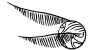
\includegraphics[scale=0.4]{boccino.png}
        \centering
\end{figure}

Quindici minuti dall’inizio dell’ora di pranzo.

Nessuno parlava con Harry. Alcuni dei Corvonero gli indirizzavano sguardi di rabbia, altri di simpatia, alcuni degli studenti più giovani ebbero persino sguardi di ammirazione, ma nessuno gli stava parlando. Anche Hermione non aveva provato ad avvicinarsi.

Fred e George si erano cautamente appropinquati. Non avevano detto niente. L’offerta era chiara, come il suo essere facoltativa. Harry aveva detto loro che sarebbe venuto al momento del dolce, non prima. Avevano annuito e si erano allontanati di fretta.

Era probabilmente l’aspetto del tutto inespressivo del volto di Harry che ci stava riuscendo.

Gli altri probabilmente pensavano che stesse controllando la rabbia, o lo sgomento. Sapevano, perché avevano visto Flitwick venirlo a prendere, che era stato convocato nell’ufficio del Preside.

Harry stava cercando di non sorridere, perché se avesse sorriso, avrebbe iniziato a ridere, e se avesse iniziato a ridere, non si sarebbe fermato fino a quando le simpatiche persone con la divisa bianca non fossero venute a portarlo via.

Era troppo. Era tutto davvero troppo. Harry era quasi passato al Lato Oscuro, il suo lato oscuro aveva fatto cose che sembravano in retrospettiva folli, il suo lato oscuro aveva vinto una vittoria impossibile che sarebbe potuta essere vera e sarebbe potuta essere un puro capriccio di un Preside folle, il suo lato oscuro aveva protetto i suoi amici. Non riusciva più a sopportarlo. Aveva bisogno che Fawkes cantasse di nuovo per lui. Aveva bisogno di usare il Giratempo per procurarsi un’ora di tranquillità per riprendersi, ma quella non era più un’opzione e la perdita era come un buco nella sua esistenza, ma non riusciva a pensarci perché altrimenti si sarebbe potuto mettere a ridere.

Venti minuti. Tutti gli studenti che avevano intenzione di mangiare a pranzo erano arrivati, quasi nessuno se n’era andato.

Il picchiettio di un cucchiaio risuonò attraverso la Sala Grande.

«Se posso avere la vostra attenzione, prego», disse Silente. «Harry Potter ha qualcosa che vuole condividere con noi.»

Harry prese un respiro profondo e si alzò. Si avvicinò al Tavolo d’onore, con tutti gli occhi che lo fissavano.

Si girò e guardò verso le quattro tavolate.

Stava diventando sempre più difficile non sorridere, ma Harry mantenne il suo volto inespressivo mentre ripeteva il suo breve discorso mandato a memoria.

«La verità è sacra», disse Harry impassibile. «Uno dei miei averi più cari è una spilla che recita ‘Di’ la verità, anche se la tua voce trema’. Questa, dunque, è la verità. Ricordatelo. Non sto dicendo questo perché sono stato obbligato a farlo, lo sto dicendo perché è vero. Ciò che ho fatto durante la lezione del professor Snape è stato folle, stupido, infantile e una violazione imperdonabile delle regole di Hogwarts. Ho disturbato la classe e privato i miei compagni del loro insostituibile tempo di apprendimento. Tutto perché non sono stato in grado di controllare il mio temperamento. Spero che non uno di voi segua mai il mio esempio. Certamente io intendo provare a non seguirlo più.»

Molti degli studenti che fissavano Harry avevano ora espressioni solenni e infelici sui loro volti, come quelle che si potrebbero vedere a una cerimonia che segni la fine di un campione sconfitto. Nella zona più giovane della tavola Grifondoro quell’espressione era quasi universale.

Finché Harry non alzò la mano.

Non l’alzò in alto. Sarebbe potuto sembrare pretenzioso. Certamente non la sollevò verso Severus. Semplicemente, Harry alzò la mano al livello del petto, e schioccò dolcemente le dita, un gesto che fu visto più che udito. Era possibile che la maggior parte del Tavolo d’onore non l’avesse visto affatto.

Quell’apparente gesto di ribellione conquistò gli improvvisi sorrisi degli studenti più giovani e dei Grifondoro, e i freddi sogghigni di superiorità dei Serpeverde, e le occhiate accigliate e preoccupate di tutti gli altri.

Harry mantenne il volto impassibile. «Grazie», disse. «Questo è tutto.»

«Grazie, signor Potter», disse il Preside. «E ora il professor Snape ha qualcosa da condividere con noi anche lui.»

Severus si alzò tranquillamente dal suo posto al Tavolo d’onore. «È stato portato alla mia attenzione», disse, «che le mie azioni hanno giocato una parte nel provocare la palesemente imperdonabile rabbia del signor Potter, e nella conseguente discussione ho compreso di aver dimenticato quanto siano facilmente feriti i sentimenti dei giovani e degli immaturi –»

Ci fu il suono di molte persone che emettevano contemporaneamente dei rantoli soffocati.

Severus continuò come se non avesse sentito. «L’aula di Pozioni è un posto pericoloso, e ritengo ancora che una rigida disciplina sia necessaria, ma per l’avvenire sarò più consapevole della… fragilità emotiva… degli studenti del quarto anno e ancor più giovani. La mia sottrazione di punti a Corvonero è ancora valida, ma revoco la detenzione del signor Potter. Grazie.»

Ci fu un singolo battito di mani proveniente dalla direzione dei Grifondoro e, più veloce di un fulmine, la bacchetta di Severus fu nella sua mano e «Quietus!» zittì il responsabile.

«Continuerò a pretendere disciplina e rispetto in tutte le mie classi», disse freddamente Severus, «e chiunque scherzasse con me se ne pentirà.»

Si sedette.

«Grazie anche a te!» disse allegramente il preside Silente. «Continuate!»

E Harry, ancora impassibile, iniziò a tornare alla propria sedia in Corvonero.

Ci fu un’esplosione di conversazioni. Due parole erano chiaramente identificabili all’inizio. La prima era un «Cosa –» iniziale, con cui cominciavano diverse frasi come «Cos’è successo –» e «Cosa diavolo –» La seconda era «Scourgify!», mentre gli studenti ripulivano il cibo caduto e le bevande che essi stessi avevano versato, dalle tovaglie e dalle vesti.

Alcuni studenti stavano apertamente piangendo. Così anche la professoressa Sprout.

Al tavolo Grifondoro, dove una torta attendeva con cinquantuno candeline non ancora accese, Fred sussurrò «Penso che questo sia davvero troppo per noi, George.»

E da quel giorno in poi, non importa cosa Hermione provasse a dire a tutti, fu una leggenda accettata di Hogwarts che Harry Potter potesse far accadere assolutamente qualunque cosa schioccando le dita.




\% !TeX root = Harry.tex



\chapter{Gratificazione differita}

\label{capitolo:19}



\emph{Draco aveva un’espressione severa sul volto, e le sue vesti bordate di verde sembravano in qualche modo molto più formali, serie, e di miglior qualità delle stesse esatte vesti indossate dai due ragazzi dietro di lui.}



~\\

~\\



«Parla», disse Draco.

«Sì! Parla!»

«Hai sentito al capo! Parla!»

«Voi due, d’altro canto, state zitti.»

L’ultima sessione di lezioni di venerdì stava per iniziare, in quel vasto auditorium dove tutte e quattro le Case imparavano Difesa, cioè, Magia da Battaglia.

L’ultima sessione di lezioni di venerdì.

Harry stava sperando che quella lezione sarebbe stata tranquilla, e che il brillante professor Quirrell avrebbe compreso che quello non era forse il momento migliore per scegliere Harry tra tanti per qualche dimostrazione. Harry si era ripreso un po’, ma…

… ma giusto per sicurezza, era probabilmente meglio alleviare un po’ la tensione, prima.

Harry si appoggiò allo schienale della sedia e accordò uno sguardo di grande solennità a Draco e ai suoi servitori.

«Voi chiedete: qual è il nostro obiettivo?» declamò Harry. «Posso rispondere con una parola. È la vittoria. Vittoria a tutti i costi — Vittoria malgrado qualunque terrore — Vittoria, per quanto lunga e dura possa essere la strada, perché senza vittoria non c’è –»

«Parla di Snape», sibilò Draco. «Che cosa hai fatto?»

Harry abbandonò la finta solennità e rivolse a Draco un’espressione più seria.

«L’hai visto. Tutti l’hanno visto. Ho schioccato le dita.»

«Harry! Smettila di prendermi in giro!»

Quindi era stato promosso a Harry ora. Interessante. E infatti, Harry era abbastanza sicuro che fosse previsto che se ne accorgesse, e si sentisse ingrato se non avesse contraccambiato in qualche modo…

Harry si toccò le orecchie e rivolse un’occhiata significativa ai servitori.

«Non parleranno», disse Draco.

«Draco», Harry disse, «sarò onesto al cento per cento e ti dirò che ieri non sono stato particolarmente impressionato dall’astuzia del signor Goyle.»

Il signor Goyle trasalì.

«Neppure io», disse Draco. «Gli ho spiegato che ho finito per doverti un favore, a causa di ciò.» (Il signor Goyle trasalì ancora.) «Ma esiste una grande differenza tra quel genere di errore e l’essere indiscreto. Questo è davvero qualcosa che sono stati addestrati a capire sin dall’infanzia.»

«Allora va bene», disse Harry. Abbassò la voce, anche se i rumori di sottofondo erano divenuti confusi in presenza di Draco. «Ho dedotto uno dei segreti di Severus e ho esercitato un piccolo ricatto.»

L’espressione di Draco si indurì. «Bene, ora dimmi qualcosa che non hai detto nella più stretta confidenza a quegli idioti in Grifondoro, il che significa che quella era la storia che volevi che fosse diffusa in tutta la scuola.»

Harry sorrise involontariamente, e seppe che Draco l’aveva notato.

«Cosa dice Severus?», chiese Harry.

«Che non si era reso conto di quanto siano sensibili i bambini piccoli», rispose Draco. «Anche in Serpeverde! Anche a me!»

«Sei sicuro», disse Harry, «che vuoi sapere qualcosa che il responsabile della tua Casa preferirebbe che non sapessi?»

«Sì», Draco disse senza esitazione.

Interessante. «Allora dovrai davvero mandare via i tuoi servitori, prima, perché non sono sicuro di poter credere a tutto ciò che tu credi riguardo a loro.»

Draco annuì. «Va bene.»

Il signor Crabbe e il signor Goyle sembrarono molto scontenti. «Capo –» disse il signor Crabbe.

«Non avete dato al signor Potter nessuna ragione per fidarsi di voi», disse Draco. «Andate!»

Se ne andarono.

«In particolare», Harry disse abbassando ancora di più la voce, «non sono completamente sicuro che non andrebbero a riferire quanto dicessi a Lucius.»

«Mio Padre non farebbe mai una cosa simile!» disse Draco sembrando genuinamente inorridito. «Sono miei!»

«Mi dispiace, Draco», Harry disse. «È solo che non sono sicuro di poter credere a tutto ciò che tu credi riguardo tuo padre. Immagina se fosse il tuo segreto e io ti dicessi che mio padre non lo farebbe.»

Draco annuì lentamente. «Hai ragione. Sono io a essere dispiaciuto. È stato un mio errore chiedertelo.»

Come ho fatto a crescere così tanto nella sua considerazione? Non dovrebbe odiarmi, ora? Harry ebbe la sensazione di stare osservando qualcosa di sfruttabile… desiderò che il suo cervello non fosse così stanco. Normalmente avrebbe provato qualche macchinazione complicata.

«A ogni modo», disse Harry. «Facciamo uno scambio. Io ti racconto un fatto che non è tra i pettegolezzi, e non finisce tra i pettegolezzi, e in particolare non arriva a tuo padre, e in cambio mi dici cosa tu e i Serpeverde pensate di tutta questa faccenda.»

«Aggiudicato!»

Ora, per metterla nella maniera più vaga possibile… in qualche modo che non avrebbe causato un danno anche se si fosse saputo… «Ciò che ho detto è vero. Ho realmente scoperto uno dei segreti di Severus e ho esercitato un piccolo ricatto. Ma Severus non era l’unica persona coinvolta.»

«Lo sapevo!» disse un Draco esultante.

Lo stomaco di Harry sprofondò. Apparentemente aveva detto qualcosa di veramente significativo e non sapeva perché. Non era un buon segno.

«Va bene», disse Draco. Ora aveva un sorriso largo. «Eccoti le reazioni in Serpeverde, allora. All’inizio, tutti gli idioti hanno detto ‘Odiamo Harry Potter! Andiamo a pestarlo!’»

Harry soffocò. «Ma cosa c’è di sbagliato nel Cappello Smistatore? Questo non è Serpeverde, è Grifondoro –»

«Non tutti i sono bambini prodigio» disse Draco, sebbene stesse sorridendo in un modo quasi complice, come a suggerire che privatamente concordava con l’opinione di Harry. «E a qualcuno ci sono voluti circa quindici secondi per spiegare loro perché questo sarebbe potuto non andare a favore di Snape, quindi sei al sicuro. Ad ogni modo, dopo c’è stata la seconda ondata di idioti, quelli che dicevano ‘Pare che Harry Potter sia un altro che vuole salvare il mondo, dopo tutto’».

«E poi?» disse Harry, sorridendo anche se non aveva idea del perché quello fosse stupido.

«E poi le persone realmente intelligenti hanno iniziato a parlare. È ovvio che hai trovato un modo per mettere parecchia pressione su Snape. E sebbene possa esserci più di un modo per farlo… l’ovvio pensiero successivo è stato che abbia qualcosa a che fare con la misteriosa influenza di Snape su Silente. Ho ragione?»

«Nessun commento», disse Harry. Almeno il suo cervello stava elaborando questa parte correttamente. In Casa Serpeverde si erano chiesti perché Severus non fosse stato licenziato. E avevano concluso che Severus stava ricattando Silente. Poteva essere vero…? Ma Silente non era sembrato agire come se fosse stato così…

Draco continuò a parlare. «E la cosa successiva che le persone intelligenti hanno sottolineato è stata che se hai potuto mettere abbastanza pressione su Snape da fargli lasciare in pace metà Hogwarts, questo significava che probabilmente avevi abbastanza potere da sbarazzarti di lui completamente, se avessi voluto. Quello che gli hai fatto è stato umiliarlo, proprio come lui ha cercato di umiliare te — ma ci hai lasciato il Preside della nostra Casa».

Harry rese il proprio sorriso più ampio.

«E poi le persone veramente intelligenti», disse Draco, il suo volto ora serio, «si sono appartate e hanno avuto una piccola discussione tra di loro, e qualcuno ha sottolineato che sarebbe stata una cosa molto stupida lasciare in giro un nemico così. Se avessi potuto spezzare la sua influenza su Silente, la cosa più ovvia sarebbe stata quella di farlo e basta. Silente avrebbe cacciato Severus via da Hogwarts e forse l’avrebbe anche fatto uccidere, ti sarebbe stato molto riconoscente, e tu non avresti dovuto preoccuparti che Severus entri furtivamente di notte nella tua stanza del dormitorio con delle pozioni interessanti.»

Il viso di Harry era ora neutro. Non ci aveva pensato, e avrebbe davvero, davvero dovuto farlo. «E da ciò avete concluso…?»

«Che l’influenza di Severus fosse un segreto di Silente e che tu conosci quel segreto!» Draco sembrava esultante. «Non può essere abbastanza potente da distruggere Silente completamente, o Snape l’avrebbe già usata. Snape rifiuta di usare la sua influenza per qualsiasi cosa eccetto restare signore incontrastato della Casa di Serpeverde di Hogwarts, e neppure in questo caso riesce sempre a ottenere ciò che vuole, quindi deve avere dei limiti. Ma deve essere veramente buona! Mio Padre sta cercando di convincere Severus a rivelargliela da anni!»

«E», disse Harry, «ora Lucius pensa che forse io potrò rivelargliela. Per caso, hai già ricevuto un gufo –»

«Lo riceverò questa sera», Draco disse, e rise. «Dirà», la sua voce assunse una cadenza differente, più formale, «Mio amato figlio: ti ho già detto della potenziale importanza di Harry Potter. Come avrai già capito, la sua importanza è diventata ora più grande e più urgente. Se notassi un possibile modo per stringere un’amicizia o per scoprire un suo punto debole, devi perseguirlo, e tutte le risorse di Malfoy sono a tua disposizione in caso di necessità.»

Accidenti. «Bene», Harry disse, «evitando ogni commento sul fatto che tutto il tuo complicato edificio teorico sia vero o meno, lasciami dire che non siamo ancora così buoni amici.»

«Lo so», disse Draco. Poi il suo viso divenne molto serio, e la sua voce si fece più bassa, malgrado i rumori esterni fossero già attutiti. «Harry, ti è mai venuto in mente che se tu sapessi qualcosa che Silente non vuole che sia risaputa, potrebbe semplicemente farti uccidere? E il Ragazzo-Che-È-Sopravvissuto passerebbe da potenziale concorrente capo-fazione a prezioso martire, persino.»

«Nessun commento», Harry disse di nuovo. Non aveva pensato neppure a quest’ultima cosa. Non sembrava essere nello stile di Silente… ma…

«Harry», riprese Draco, «è evidente che tu possegga un talento impressionante, ma non hai alcun addestramento né un mentore, e commetti davvero delle stupidaggini, talvolta, e hai davvero bisogno di un consigliere che sappia come si fa, o ti farai male!» Il volto di Draco era feroce.

«Ah», disse Harry. «Un consigliere come Lucius?»

«Come me!» rispose Draco. «Ti prometto di mantenere i tuoi segreti con mio Padre, con chiunque, mi limiterò ad aiutarti a capire quello che vuoi fare!»

Uau.

Harry vide zombi-Quirrell che attraversava barcollando le porte.

«La lezione sta per iniziare», disse Harry. «Penserò a quello che mi hai detto, parecchie volte mi capita di desiderare di aver ricevuto tutto il tuo addestramento, è solo che non so come posso fidarmi di te così in fretta –»

«Non dovresti», disse Draco, «è troppo presto. Vedi? Ti darò buoni consigli anche se mi danneggiano. Ma forse dovremmo affrettarci e diventare amici più intimi.»

«Sono aperto a questa proposta», disse Harry, che stava già cercando di capire come sfruttarla.

«Un altro piccolo consiglio», disse Draco frettolosamente mentre Quirrell si trascinava verso la cattedra, «in questo momento in Serpeverde tutti si interrogano su di te, quindi se ci stai corteggiando, cosa che penso tu stia facendo, dovresti compiere qualche gesto che sia un segnale di amicizia verso Serpeverde. Presto, tipo oggi o domani.»

«Permettere che Severus continui ad assegnare punti-Casa supplementari a Serpeverde non è stato sufficiente?» Non c’era ragione per cui Harry non si prendesse il merito di quello.

Le palpebre di Draco batterono per la comprensione, poi egli disse rapidamente, «Non è la stessa cosa, credimi, deve essere qualcosa di ovvio. Spingi contro un muro la tua rivale sanguemarcio Granger o qualcosa del genere, tutti in Serpeverde capiranno cosa significa –»

«Non è così che funziona in Corvonero, Draco! Se devi spingere qualcuno contro un muro significa che il tuo cervello è troppo debole per batterlo nel modo giusto e dentro Corvonero lo sanno tutti –»

Lo schermo sulla scrivania di Harry si accese con uno sfarfallio, causando un’improvvisa ondata di nostalgia per la televisione e i computer.

«Ehm», disse la voce del professor Quirrell, che sembrò parlare personalmente a Harry dallo schermo. «Prego, raggiungete i vostri posti.»

\begin{figure}[h!]
        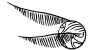
\includegraphics[scale=0.4]{boccino.png}
        \centering
\end{figure}

E i bambini erano tutti seduti a guardare gli schermi ripetitori sui loro banchi, o a guardare in basso direttamente al grande palcoscenico di marmo bianco, su cui il professor Quirrell stava in piedi, appoggiato alla sua cattedra in cima alla piccola pedana di marmo scuro.

«Oggi», disse il professor Quirrell, «avevo previsto di insegnarvi il vostro primo incantesimo difensivo, un piccolo scudo che fu l’antenato del Protego odierno. Ma riflettendoci, ho cambiato il programma della lezione di oggi alla luce dei recenti avvenimenti.»

Lo sguardo del professor Quirrell cercò tra le file di sedili. Là dove era seduto, in ultima fila, Harry fece una smorfia. Aveva la sensazione di sapere chi stava per essere chiamato.

«Draco, della Nobile e Antichissima Casa Malfoy», disse il professor Quirrell.

Scampata.

«Sì, professore?» disse Draco. La sua voce era amplificata, e proveniva apparentemente dallo schermo ripetitore sul banco di Harry, che mostrava il volto di Draco mentre parlava. Poi lo schermo tornò al professor Quirrell, che disse:

«È sua ambizione diventare il prossimo Signore Oscuro?»

«Questa è una domanda strana, professore», disse Draco. «Voglio dire, chi sarebbe così stupido da ammetterlo?»

Alcuni studenti risero, ma non molti.

«Infatti», disse il professor Quirrell. «Ma sebbene sia inutile chiederlo a qualcuno di voi, non mi sorprenderebbe minimamente se ci fossero uno studente o due nelle mie classi che nutrissero l’ambizione di essere il prossimo Signore Oscuro. Dopo tutto, io volevo essere il prossimo Signore Oscuro, quando ero un giovane Serpeverde.»

Questa volta la risata fu molto più diffusa.

«Beh, dopo tutto è la Casa degli ambiziosi», disse il professor Quirrell, sorridendo. «Mi resi conto solo più tardi che quello che mi piaceva davvero era la Magia da Battaglia, e che la mia vera ambizione era di diventare un grande mago da combattimento e un giorno insegnare a Hogwarts. In ogni caso, quando avevo tredici anni, lessi attentamente le sezioni storiche della biblioteca di Hogwarts, vagliando le vite e i destini dei passati Signori Oscuri, e feci una lista di tutti gli errori che io non avrei mai fatto quando fossi diventato un Signore Oscuro –»

Harry ridacchiò prima di riuscire a trattenersi.

«Sì, signor Potter, molto divertente. Allora, signor Potter, può indovinare quale fosse il primo elemento in assoluto su quella lista?»

Grande. «Uhm… non usare mai un modo complicato di affrontare un nemico quando puoi semplicemente lanciargli contro un Abracadabra?»

«Le parole, signor Potter, sono Avada Kedavra», la voce del professor Quirrell suonò un po’ brusca, per qualche motivo, «e no, quello non era sulla lista che stilai all’età di tredici anni. Le andrebbe di provare di nuovo?»

«Ah… mai vantarsi con nessuno del tuo piano malvagio?»

Il professor Quirrell rise. «Ah, beh quello era al numero due. Accidenti, signor Potter, abbiamo forse letto gli stessi libri?»

Ci furono più risate, con una venatura di nervosismo. Harry serrò la mascella e non disse niente. Una smentita non sarebbe servita a nulla.

«Ma no. Il primo elemento era, ‘Non me ne andrò in giro a provocare nemici forti e feroci’. La storia del mondo sarebbe molto diversa se Mornelithe Falconsbane o Hitler avessero compreso questo punto elementare. Ora se, signor Potter — solo se per caso lei nutrisse un’ambizione simile a quella che io avevo da giovane Serpeverde — anche in quel caso, spero non sia sua ambizione diventare un Signore Oscuro stupido.»

«Professor Quirrell», disse Harry digrignando i denti, «io sono un Corvonero e non è mia ambizione essere stupido, punto. So che ciò che ho fatto oggi era sciocco. Ma non era Oscuro! Non sono stato io a dare il primo pugno in quello scontro!»

«Lei, signor Potter, è un idiota. Ma del resto lo ero anch’io alla sua età. Così ho anticipato la sua risposta e mutato di conseguenza il piano della lezione di oggi. Signor Gregory Goyle, vorrebbe farsi avanti, per cortesia?»

Ci fu una pausa sorpresa nell’aula. Harry non se l’aspettava.

Né, a quanto pare, se l’aspettava il signor Goyle, che sembrò piuttosto incerto e preoccupato mentre salì sul palco di marmo e si avvicinò alla pedana.

Il professor Quirrell si raddrizzò allontanandosi dalla scrivania su cui si era appoggiato. Sembrò improvvisamente più forte, le sue mani si strinsero a pugno e assunse una posa da arti marziali chiaramente riconoscibile.

A quella vista, gli occhi di Harry si spalancarono, e comprese perché il signor Goyle era stato chiamato.

«La maggior parte dei maghi», disse il professor Quirrell, «non sprecano molto tempo con quelle che un Babbano chiamerebbe arti marziali. Non è forse una bacchetta più forte di un pugno? Questo atteggiamento è stupido. Le bacchette sono strette nei pugni. Se volete essere un grande mago da combattimento dovete imparare le arti marziali a un livello tale da impressionare anche un Babbano. Passo ora a dare prova di una certa tecnica di vitale importanza, che ho appreso in un dojo, una scuola babbana di arti marziali, di cui parlerò tra breve. Per ora…» Il professor Quirrell fece alcuni passi in avanti, ancora in posizione, avanzando verso il luogo dove era il signor Goyle. «Signor Goyle, le chiedo di attaccarmi.»

«Professor Quirrell», disse il signor Goyle, la sua voce ora amplificata come quella del professore, «posso chiederle a che livello –»

«Sesto dan. Non si farà del male e neppure me ne farò io. E se vede un varco, la prego di sfruttarlo.»

Il signor Goyle annuì, sembrando molto sollevato.

«Notate», disse il professor Quirrell, «che il signor Goyle aveva paura di attaccare qualcuno che non conoscesse le arti marziali a un livello accettabile, per timore che io, o lui, ci saremmo fatti male. L’atteggiamento del signor Goyle è perfettamente corretto e perciò si è guadagnato tre punti-Quirrell. Ora, attacchi!»

Il giovane ragazzo si gettò avanti, pugni in aria, e il professore bloccò ogni colpo, danzando all’indietro, Quirrell calciò e Goyle bloccò e si girò, e cercò far inciampare Quirrell spazzando con la gamba e Quirrell la scavalcò e tutto stava accadendo troppo in fretta perché Harry potesse dare un senso a quello che succedeva e poi Goyle fu sulla propria schiena con le gambe che spingevano e Quirrell letteralmente volò per aria e poi colpì terra con la spalla e rotolò via.

«Fermo!» gridò il professor Quirrell da terra, suonando un po’ impaurito. «Ha vinto!»

Il signor Goyle si fermò così bruscamente che barcollò, quasi inciampando e cadendo a causa del momento abortito della sua carica a testa bassa verso il professor Quirrell. Il suo volto mostrava un completo disorientamento.

Il professor Quirrell inarcò la schiena e si rialzò in piedi usando un peculiare movimento a molla che non faceva uso di mani.

Ci fu silenzio in aula, un silenzio nato dalla completa confusione.

«Signor Goyle», disse il professor Quirrell, «quale tecnica di importanza vitale ho dimostrato?»

«Come cadere in maniera corretta quando si è proiettati da qualcuno», disse il signor Goyle. «È una delle prime lezioni che si imparano –»

«Anche quella», disse il professor Quirrell.

Ci fu una pausa.

«La tecnica di importanza vitale che ho dimostrato», disse il professor Quirrell, «è stata come perdere. Può andare, signor Goyle, grazie.»

Il signor Goyle abbandonò la piattaforma, sembrando alquanto frastornato. Harry si sentiva nello stesso modo.

Il professor Quirrell tornò alla cattedra e riprese ad appoggiarcisi. «A volte dimentichiamo le cose più elementari, dal momento che è passato troppo tempo da quando le abbiamo imparate. Mi sono accorto che ho fatto lo stesso con il mio programma di lezioni. Non insegni agli studenti a lanciare fino a quando non hai insegnato loro a cadere. E non devo insegnarvi a combattere se non sapete come perdere.»

Il volto del professor Quirrell si indurì, e Harry credette di vedere un accenno di dolore, un tocco di tristezza, in quegli occhi. «Ho imparato a perdere in un dojo in Asia, che, come ogni Babbano sa, è dove vivono tutti i bravi praticanti di arti marziali. Questo dojo insegnava uno stile che tra i maghi da combattimento aveva la reputazione di adattarsi bene al duello di magia. Il Maestro di quel dojo — un uomo anziano secondo i criteri babbani — era il più grande maestro vivente di tale stile. Non aveva idea dell’esistenza della magia, ovviamente. Feci richiesta di studiare lì, e fui uno dei pochi allievi ammessi per quell’anno, tra i tanti candidati. In quella decisione potrebbe aver giocato un ruolo un po’ di condizionamento speciale.»

Ci furono alcune risate dalla classe. Harry non le condivise. Quell’atto non era stato affatto corretto.

«Ad ogni modo. Durante uno dei miei primi combattimenti, dopo che ero stato battuto in un modo particolarmente umiliante, persi il controllo e attaccai il mio avversario –»

Accidenti.

«– per fortuna con i pugni, piuttosto che con la magia. Il Maestro, sorprendentemente, non mi espulse immediatamente. Ma mi disse che c’era un difetto nel mio temperamento. Me lo spiegò, e io seppi che aveva ragione. E poi mi disse che avrei dovuto imparare a perdere.»

Il volto del professor Quirrell era inespressivo.

«Dietro suoi precisi ordini, tutti gli allievi del dojo si misero in fila. Uno per uno, si avvicinarono a me. Il mio ordine era di non difendermi. Dovevo solo chiedere pietà. Uno per uno, mi schiaffeggiarono, o mi diedero un pugno, e mi spinsero a terra. Alcuni di loro mi sputarono addosso. Mi chiamarono con nomi terribili nella loro lingua. E a ciascuno di loro, dovevo dire ‘ho perso!’ e cose simili, come ad esempio ‘ti prego di smetterla!’ e ‘riconosco che sei migliore di me!’»

Harry stava cercando di immaginare la scena e semplicemente non ci riusciva. Non c’era modo che una cosa del genere fosse potuta accadere al fiero professor Quirrell.

«Già allora ero un prodigio in Magia da Battaglia. Solo con la magia senza bacchetta avrei potuto uccidere tutti, in quel dojo. Non lo feci. Imparai a perdere. Fino a oggi me la ricordo come una delle ore più sgradevoli della mia vita. E quando lasciai quel dojo otto mesi dopo — che non furono neppure lontanamente sufficienti, ma erano tutto il tempo che potevo permettermi di passare lì — il Maestro mi disse che sperava avessi compreso perché era stato necessario. E gli risposi che era una delle lezioni più preziose che avessi mai imparato. Cosa che era, ed è, vera.»

L’espressione del professor Quirrell divenne più amara. «Vi starete chiedendo dove sia questo meraviglioso dojo, e se possiate studiare lì. Non potete. Perché non molto tempo dopo, un altro potenziale allievo giunse in quel luogo nascosto, in quella remota montagna. Colui-Che-Non-Deve-Essere-Nominato.»

Ci fu il suono di molte inspirazioni simultanee. Harry sentì una stretta allo stomaco. Sapeva cosa stava per accadere.

«Il Signore Oscuro giunse in quella scuola apertamente, senza travestimento, con gli occhi che brillavano di rosso e tutto il resto. Gli allievi tentarono di ostacolare il suo ingresso ed egli, semplicemente, li superò Materializzandosi. Ci fu terrore, ma anche disciplina, e il Maestro si fece avanti. E il Signore Oscuro pretese — non chiese, ma pretese — che gli insegnasse.»

L’espressione del professor Quirrell era molto dura. «Forse il Maestro aveva letto troppi libri che raccontavano la bugia che un vero praticante di arti marziali può sconfiggere anche i demoni. Qualunque fosse la ragione, il Maestro rifiutò. Il Signore Oscuro chiese perché non potesse essere un allievo. Il Maestro rispose che non aveva pazienza, e fu allora che il Signore Oscuro gli strappò la lingua.»

Ci fu un sussulto collettivo.

«Potete indovinare che cosa è successo dopo. Gli allievi cercarono di avventarsi sul Signore Oscuro e caddero, storditi sul posto. E poi…»

La voce del professor Quirrell esitò per un momento, poi riprese.

«C’è una Maledizione Senza Perdono, la Maledizione Cruciatus, che produce un dolore insopportabile. Se la Cruciatus è mantenuta per più di qualche minuto produce una pazzia permanente. Uno a uno, il Signore Oscuro sottopose gli allievi del Maestro al Cruciatus fino alla follia, e poi li finì con la Maledizione Mortale, mentre il Maestro fu costretto a guardare. Quando tutti i suoi allievi furono morti in questo modo, il Maestro li seguì. Ho imparato tutto ciò dall’unico allievo sopravvissuto, che il Signore Oscuro lasciò in vita per raccontare la storia, e che era stato un mio amico…»

Il professor Quirrell si voltò, e quando si rigirò un momento dopo, sembrò ancora una volta calmo e composto.

«I Maghi Oscuri non riescono a controllare il proprio temperamento», disse con calma il professor Quirrell. «È un difetto quasi universale della loro specie, e chiunque faccia l’abitudine a combatterli impara presto a farvi affidamento. Dovete comprendere che quel giorno il Signore Oscuro non vinse. Il suo scopo era imparare le arti marziali, eppure se ne andò senza una sola lezione. Il Signore Oscuro fu folle a volere che quella storia fosse raccontata. Non mostrò la sua forza, ma piuttosto una debolezza sfruttabile.»

Lo sguardo del professor Quirrell si focalizzò su di un singolo bambino nell’aula.

«Harry Potter», disse il professor Quirrell.

«Sì», disse Harry, la sua voce roca.

«In cosa esattamente ha sbagliato oggi, signor Potter?»

Harry si sentiva come se stesse per vomitare. «Ho perso la calma.»

«Questo non è preciso», disse il professor Quirrell. «Lo descriverò più precisamente. Ci sono molte specie animali in cui si praticano i cosiddetti giochi di dominanza. Si scontrano impattando con le corna — cercando di buttarsi giù a vicenda, non di trafiggersi l’un l’altro. Combattono con le zampe — con gli artigli retratti. Ma perché con gli artigli retratti? Sicuramente, se usassero gli artigli, avrebbero una probabilità maggiore di vincere, no? Ma in quel caso il loro avversario potrebbe ugualmente sfoderare gli artigli, e invece di risolvere il gioco di dominanza con un vincitore e un perdente, entrambi potrebbe essere gravemente feriti.»

Lo sguardo del professor Quirrell sembrò puntare dallo schermo ripetitore direttamente a Harry. «Quello che ha dimostrato oggi, signor Potter, è che — a differenza di quegli animali che tengono i loro artigli retratti e accettano i verdetti — lei non sa come perdere un gioco di dominanza. Quando un professore di Hogwarts l’ha sfidata, lei non si è tirato indietro. Quando è sembrato che potesse perdere, lei ha tirato fuori gli artigli noncurante del pericolo. Lei ha intensificato lo scontro, e dopo l’ha intensificato ancora. È iniziato con uno schiaffo datole dal professor Snape, che era ovviamente dominante su di lei. Invece di perdere, lei ha restituito lo schiaffo e ha perso dieci punti per Corvonero. Poco dopo stava parlando di lasciare Hogwarts. Il fatto che lei abbia intensificato il conflitto ancor di più in una direzione sconosciuta, e in qualche modo alla fine abbia vinto, non cambia il fatto che lei sia un idiota.»

«Comprendo», disse Harry. La sua gola era secca. Era stato preciso. Spaventosamente preciso. Ora che il professor Quirrell l’aveva esposta, Harry poteva vedere col senno di poi che quella era una descrizione accurata di ciò che era successo. Quando il modello che qualcuno ha di te è così buono, devi chiederti se abbia ragione anche a proposito di altro, come la tua volontà di uccidere.

«La prossima volta, signor Potter, che sceglierà di intensificare uno scontro piuttosto che ammettere la sconfitta, lei potrebbe perdere l’intera posta in gioco. Non so quale fosse quella di oggi. So che era molto, molto più importante della perdita di dieci punti-Casa.»

Come il destino della Gran Bretagna magica. Quello era ciò che aveva fatto.

«Protesterà dicendo che stava cercando di aiutare l’intera Hogwarts, uno scopo ben più importante e degno di maggiori rischi. Questa è una bugia. Se fosse stato questo –»

«Avrei incassato lo schiaffo, atteso, e scelto il miglior momento possibile per fare la mia mossa», disse Harry, la sua voce roca. «Ma questo avrebbe significato perdere. Permettergli di dominarmi. Questo è quello che il Signore Oscuro non è stato in grado di fare col Maestro da cui voleva imparare.»

Il professor Quirrell annuì. «Vedo che ha compreso perfettamente. E quindi, signor Potter, oggi lei imparerà come perdere.»

«Io –»

«Non voglio sentire obiezioni, signor Potter. È evidente che lei ne abbia bisogno, e che è abbastanza forte da sopportarlo. Le assicuro che la sua esperienza non sarà così severa come quella che ho dovuto affrontare io, sebbene potrebbe ricordarseli come i peggiori quindici minuti della sua giovane vita.»

Harry deglutì. «Professor Quirrell», disse a voce bassa, «potremmo farlo un’altra volta?»

«No», rispose semplicemente il professor Quirrell. «Lei è al quinto giorno dei suoi studi a Hogwarts ed è già accaduto tutto questo. Oggi è venerdì. La nostra prossima lezione di difesa è mercoledì. Sabato, domenica, lunedì, martedì, mercoledì… No, non abbiamo il tempo per aspettare.»

Ci furono poche risate in risposta, ma davvero poche.

«La prego di considerarlo un ordine del suo professore, signor Potter. Quello che vorrei dirle è che in caso contrario non le insegnerò alcun incantesimo d’attacco, perché verrei poi a sapere che ha gravemente ferito o persino ucciso qualcuno. Sfortunatamente mi dicono che le sue dita sono già armi potenti. Non le schiocchi mai durante questa lezione.»

Altre risate sparpagliate, dal tono alquanto nervoso.

Harry sentì di potersi mettere a piangere. «Professor Quirrell, se farà qualcosa come quello che ha descritto, mi arrabbierò, e davvero preferirei non arrabbiarmi ancora, oggi –»

«Il punto non è evitare di arrabbiarsi», disse il professor Quirrell, il suo volto severo. «La rabbia è naturale. Deve imparare come perdere anche quando è arrabbiato. O almeno fingere di perdere così da poter progettare la sua vendetta. Come ho fatto io oggi col signor Goyle, a meno che qualcuno di voi non creda che sia davvero migliore di me –»

«Io no!» gridò il signor Goyle dal suo banco, sembrando un po’ agitato. «Io so che non ha realmente perso! La prego, non mediti nessuna vendetta!»

Harry sentì una stretta allo stomaco. Il professor Quirrell non era a conoscenza del suo misterioso lato oscuro. «Professore, è realmente necessario che ne discutiamo dopo la lezione –»

«Lo faremo», promise il professor Quirrell. «Dopo che avrà imparato come si perde.» Il suo volto era serio. «Inutile dire che eviterò qualunque cosa che potrebbe ferirla o persino causarle un forte dolore. Il dolore sarà causato dalla difficoltà di perdere, invece di combattere a sua volta e intensificare lo scontro fino alla vittoria.»

Il respiro di Harry si ruppe in brevi e terrorizzati ansimi. Era più spaventato ora di quanto fosse stato lasciando la lezione di Pozioni. «Professor Quirrell», riuscì a dire, «non voglio che lei sia licenziato per questo –»

«Non lo sarò», disse il professor Quirrell, «se dopo lei dirà che è stato necessario. E sono fiducioso che lo farà.» Per un momento la voce del professor Quirrell divenne secca. «Mi creda, hanno tollerato ben peggio nei loro corridoi. Questo caso sarà eccezionale solo perché avrà luogo in aula.»

«Professor Quirrell», sussurrò Harry, ma pensò che la sua voce fosse ancora trasmessa ovunque, «ritiene davvero che se non lo facessi, potrei far del male a qualcuno?»

«Sì», disse semplicemente il professor Quirrell.

«Allora», Harry sentiva la nausea crescere, «lo farò.»

Il professor Quirrell si girò a considerare i Serpeverde. «Dunque… con la piena approvazione del vostro professore, e in maniera tale che Snape non possa essere biasimato per le vostre azioni… qualcuno di voi desidera mostrare la propria supremazia sul Ragazzo-Che-È-Sopravvissuto? Spintonarlo, buttarlo a terra, ascoltarlo mentre implora la vostra pietà?»

Cinque mani si alzarono.

«Tutti quelli con la mano alzata sono dei completi idioti. Quale parte di fingere di perdere non avete compreso? Se Harry Potter diventasse realmente il prossimo Signore Oscuro, vi darà la caccia e vi ucciderà dopo che si sarà diplomato.»

Le cinque mani scesero repentinamente sui banchi.

«Non lo farò», disse Harry, la sua voce uscì piuttosto debole. «Giuro che non mi vendicherò mai di coloro che mi aiuteranno a imparare a perdere. Professor Quirrell… la prego… smetterebbe di fare così?»

Il professor Quirrell sospirò. «Sono davvero dispiaciuto, signor Potter. Comprendo che debba trovare tutto questo molto seccante, che intenda diventare un Signore Oscuro o meno. Ma anche quei bambini hanno un’importante lezione di vita da imparare. Sarebbe accettabile se le concedessi un punto-Quirrell per scusarmi?»

«Facciamo due», Harry disse.

Ci fu un’onda di risate sorprese, che sdrammatizzarono un po’ della tensione.

«Fatto», disse il professor Quirrell.

«E dopo che mi sarò diplomato vi darò la caccia e vi farò il solletico.»

Ci furono altre risate, sebbene il professor Quirrell non sorridesse.

Harry si sentì come se stesse combattendo contro un anaconda, cercando di obbligare la conversazione all’interno di uno stretto percorso che avrebbe fatto comprendere alle persone che non era un Signore Oscuro, dopo tutto… perché il professor Quirrell sospettava di lui?

«Professore», disse la voce non amplificata di Draco. «Diventare un Signore Oscuro stupido non è neppure una mia ambizione.»

Ci fu un silenzio sconcertato nell’aula.

Non sei obbligato a farlo! scappò quasi dalla bocca di Harry, ma si controllò in tempo; Draco avrebbe potuto desiderare che non fosse noto che lo stava facendo per la sua amicizia con Harry… o per il suo desiderio di sembrare amico…

Aver chiamato quel gesto un desiderio di sembrare amico fece sentire Harry piccolo, e meschino. Se Draco aveva inteso impressionarlo, ci stava riuscendo perfettamente.

Il professor Quirrell stava considerando Draco con serietà. «Lei dubita di non essere in grado di fingere, signor Malfoy? Che questo difetto che descrive il signor Potter descriva anche lei? Certamente suo padre sarà stato in grado di insegnarglielo.»

«Quando si tratta di discutere, forse», disse Draco, ora sullo schermo ripetitore. «Non quando si tratta di essere spintonato e gettato a terra. Voglio essere forte proprio come lei, professor Quirrell.»

Le sopracciglia del professor Quirrell si alzarono e rimasero su. «Sono spiacente, signor Malfoy», disse dopo un po’ di tempo, «gli accordi che ho preso per il signor Potter, e che coinvolgono alcuni Serpeverde più grandi a cui sarà detto solo dopo quanto siano stati stupidi, non si possono applicare a lei. Ma è mia opinione professionale che lei sia già molto forte. Dovessi venire a sapere che lei ha fallito, come ha fallito oggi il signor Potter, prenderò gli accordi appropriati e chiederò scusa a lei e a chiunque avesse ferito. Non penso che questo sarà necessario, ad ogni modo.»

«Capisco, Professore», disse Draco.

Il professor Quirrell diede un’occhiata alla classe. «Qualcun altro desidera diventare forte?»

Alcuni studenti si guardarono in giro nervosamente. Alcuni, pensò Harry dall’ultima fila, sembrarono aprire la bocca, ma non dire nulla. Alla fine, nessuno parlò.

«Draco Malfoy sarà uno dei generali degli eserciti del vostro anno», disse il professor Quirrell, «se dovesse compiacersi di prendere parte a quell’attività dopo-scuola. E ora, signor Potter, la prego di venire avanti.»

\begin{figure}[h!]
        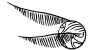
\includegraphics[scale=0.4]{boccino.png}
        \centering
\end{figure}

Sì, aveva detto il professor Quirrell, deve essere di fronte a tutti, di fronte ai suoi amici, perché è lì che Snape l’ha affrontata ed è lì che deve imparare a perdere.

Così ora l’intero primo anno stava guardando. In un silenzio imposto magicamente, e con la richiesta sia di Harry sia del professore di non intervenire. Hermione aveva girato il viso per non vedere, ma non aveva parlato o anche solo indirizzato a Harry un’occhiata significativa, forse perché anche lei era stata presente a Pozioni.

Harry era in piedi su di un morbido tappeto blu, come se ne trovavano in un dojo babbano, che il professor Quirrell aveva disposto sul pavimento per quando Harry fosse stato gettato a terra.

Harry aveva paura di quello che avrebbe potuto fare. Se il professor Quirrell aveva ragione circa la sua volontà di uccidere…

La bacchetta di Harry era poggiata sulla cattedra del professor Quirrell, non perché Harry conoscesse qualche incantesimo con cui difendersi, ma perché altrimenti (pensò Harry) avrebbe potuto cercare di spingerla attraverso l’orbita oculare di qualcuno. Anche la sua borsa giaceva lì, con all’interno il suo Giratempo, ora protetto ma ancora potenzialmente fragile.

Harry aveva implorato il professor Quirrell di Trasfigurare dei guantoni e fissarglieli alle mani. Il professor Quirrell gli aveva rivolto uno sguardo di muta comprensione, e aveva rifiutato.

Non colpirò i loro occhi, non colpirò i loro occhi, non colpirò i loro occhi, sarebbe la fine della mia vita a Hogwarts, verrei arrestato, Harry recitò a sé stesso, cercando di imprimere quel pensiero nella propria mente, sperando che rimanesse lì se la sua volontà di uccidere avesse preso il sopravvento.

Il professor Quirrell tornò, scortando tredici Serpeverde più grandi, di vari anni. Harry riconobbe uno di loro come quello che aveva colpito con una torta. C’erano altri due presenti a quel confronto. Quello che aveva detto di fermarsi, che davvero non dovevano farlo, mancava.

«Ripeto», disse il professor Quirrell con un tono molto severo, «non dovete fare realmente del male a Potter. Qualunque incidente sarà considerato intenzionale. Avete capito?»

I Serpeverde più grandi annuirono, sogghignando.

«Allora sentitevi liberi di fargli abbassare un po’ la cresta», disse il professor Quirrell, con un sorriso contorto che solo quelli del primo anno compresero.

Per una qualche sorta di accordo, la vittima del lancio della torta era in testa al gruppo.

«Potter», disse il professor Quirrell, «le presento il signor Peregrine Derrick. È migliore di lei e sta per dimostrarglielo.»

Derrick avanzò a grandi passi e il cervello di Harry urlò in maniera dissonante, non doveva scappare, non doveva reagire –

Derrick si fermò a un passo di distanza da Harry.

Harry non era ancora arrabbiato, solo spaventato. E questo significò che vide un ragazzo un mezzo metro abbondante più alto di lui, con muscoli ben definiti, peluria sul viso, e un sorriso di terrificante trepidazione.

«Gli chieda di non farle del male», disse il professor Quirrell. «Forse se la trovasse abbastanza commovente, potrebbe decidere che lei non è interessante e andarsene.»

Dai Serpeverde più grandi che stavano guardando giunse una risata.

«Ti prego», disse Harry, la sua voce tremante, «non, farmi, del, male,…»

«Non sembrava molto sincero», disse il professor Quirrell.

Il sorriso di Derrick si allargò. Quel goffo imbecille sembrava molto borioso e…

… la temperatura del sangue di Harry stava scendendo…

«Ti prego, non farmi del male», Harry tentò di nuovo.

Il professor Quirrell scosse la testa. «In nome di Merlino, come ha fatto a farlo sembrare un insulto, Potter? C’è soltanto una risposta possibile che si può attendere dal signor Derrick.»

Derrick si fece avanti, e urtò deliberatamente Harry.

Harry barcollò all’indietro per qualche metro e, prima di riuscire a impedirselo, si raddrizzò gelidamente.

«Sbagliato», disse il professor Quirrell, «sbagliato, sbagliato, sbagliato.»

«Mi hai urtato, Potter», lo accusò Derrick. «Scusati.»

«Mi dispiace!»

«Non sembri dispiaciuto», rispose Derrick.

Gli occhi di Harry si spalancarono per l’indignazione, era riuscito a farla sembrare una supplica –

Derrick lo spinse, duramente, e Harry cadde al tappeto sulle mani e sulle ginocchia.

Il tessuto blu sembrò ondeggiare davanti agli occhi di Harry, non troppo lontano.

Stava cominciando a dubitare delle reali motivazioni del professor Quirrell nell’insegnare quella cosiddetta lezione.

Un piede poggiò sulle natiche di Harry, che un attimo dopo fu spinto di lato con forza, finendo disteso sulla schiena.

Derrick rise. «È divertente», disse.

Tutto quello che doveva fare era dire che era finita lì. E segnalare l’intera faccenda all’ufficio del Preside. Sarebbe stata la fine di questo Professore di Difesa e del suo sventurato soggiorno a Hogwarts e… la professoressa McGonagall si sarebbe arrabbiata per questo, ma…

(Un’immagine del volto della professoressa McGonagall balenò davanti ai suoi occhi, non sembrava arrabbiata, solo triste –)

«Ora gli dica che è meglio di lei, Potter», disse la voce del professor Quirrell.

«Tu sei, meglio, di, me.»

Harry iniziò a sollevarsi e Derrick gli messe un piede sul petto e lo spinse di nuovo giù sul tappeto.

Il mondo stava diventando trasparente come un cristallo. Le possibili linee di azione e le loro conseguenze si dipanarono davanti ai suoi occhi in assoluta chiarezza. Lo stolto non si aspettava che lo attaccasse a sua volta, un rapido colpo all’inguine l’avrebbe stordito abbastanza a lungo per –

«Provi ancora», disse il professor Quirrell e con un improvviso movimento deciso Harry rotolò e balzò in piedi e si girò di scatto verso la direzione in cui si trovava il suo vero nemico, il Professore di Difesa –

Il professor Quirrell disse, «Lei non ha pazienza».

Harry vacillò. La sua mente, addestrata al pessimismo, disegnò l’immagine di un vecchio raggrinzito col sangue che sgorgava dalla bocca dopo che Harry gli aveva strappato via la lingua –

Un momento dopo, Derrick spinse Harry nuovamente al tappeto e poi si sedette su di lui, facendo espellere il fiato a Harry con un sibilo.

«Smettila!» Harry urlò. «Ti prego, smettila!»

«Meglio», disse il professor Quirrell. «Questa volta sembrava persino sincero.»

Era stato sincero. Quella era la cosa orribile, la cosa nauseante, che era stato sincero. Harry ansimava freneticamente, la paura e la rabbia fredda che scorrevano entrambe attraverso di lui –

«Perdi», disse il professor Quirrell.

«Io, ho perso», Harry si costrinse a dire.

«Mi piace», disse Derrick sopra di lui. «Perdi ancora.»

\begin{figure}[h!]
        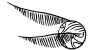
\includegraphics[scale=0.4]{boccino.png}
        \centering
\end{figure}

Delle mani spintonarono Harry, mandandolo a incespicare dall’altra parte del cerchio dei Serpeverde più grandi verso altre mani che lo spintonarono nuovamente. Harry aveva già smesso da parecchio di provare a non piangere, e ora stava semplicemente provando a non cadere a terra.

«Cosa sei tu, Potter?» chiese Derrick.

«Un, p-perdente, ho p-perso, mi arrendo, avete vinto, siete migliori, d-di me, vi prego, smettetela –»

Harry inciampò su di un piede e andò a schiantarsi al suolo, le mani incapaci di proteggerlo completamente. Rimase stordito per un attimo, poi cominciò ad alzarsi faticosamente in piedi –

«Basta!» disse la voce del professor Quirrell, un ordine così affilato da tagliare il ferro. «Allontanatevi dal signor Potter!»

Harry vide le espressioni sorprese dei loro volti. Il gelo nel suo sangue, che era montato e defluito, sorrise in fredda soddisfazione.

Poi Harry crollò sul tappeto.

Il professor Quirrell parlò. Si udirono sussulti provenire dai Serpeverde più grandi.

«E credo che anche il rampollo dei Malfoy abbia qualcosa che vuole spiegarvi», terminò il professor Quirrell.

La voce di Draco cominciò a parlare. Risuonava tagliente quasi quanto quella del professor Quirrell, aveva acquisito la stessa cadenza che Draco aveva usato per imitare suo padre, e stava dicendo cose come avrebbe potuto mettere in pericolo la Casa di Serpeverde e chissà quanti alleati solamente in questa scuola e totale mancanza di consapevolezza, per non dire di astuzia e scialbi delinquenti, buoni solo come lacchè e qualcosa nei recessi del cervello di Harry, nonostante tutto ciò che sapeva, stava designando Draco come un alleato.

A Harry faceva male tutto, era stato probabilmente ferito, il suo corpo sentiva freddo, la sua mente era completamente esausta. Cercò di pensare alla canzone di Fawkes, ma senza la fenice presente non riusciva a ricordare la melodia e quando provò a immaginarla non fu in grado di pensare ad altro che al cinguettio di un uccello.

Poi Draco smise di parlare e il professor Quirrell disse ai Serpeverde più grandi che potevano andare, e Harry aprì gli occhi e si sforzò di mettersi a sedere, «Aspetti», disse forzando le parole, «c’è qualcosa che… voglio… dire… loro –»

«Aspettate il signor Potter», il professor Quirrell ordinò freddamente ai Serpeverde che si stavano allontanando.

Harry si alzò in piedi barcollando. Fece attenzione a non guardare in direzione dei suoi compagni di classe. Non voleva vedere come lo stavano guardando ora. Non voleva vedere la loro compassione.

Quindi, invece, Harry guardò i Serpeverde più grandi, che sembravano essere ancora sconvolti. Lo fissavano. Sui loro volti il timore.

Il suo lato oscuro, mentre aveva avuto il controllo, si era sorretto sulla fantasia di quel momento, ed era riuscito a fingere di perdere.

Harry parlò, «Nessuno –»

«Fermo», disse il professor Quirrell. «Se si tratta di quello che penso, la prego di attendere che se ne siano andati. Lo sentiranno dopo. Tutti noi abbiamo le nostre lezioni da imparare, signor Potter.»

«Va bene», concesse Harry.

«Voi. Andate.»

I Serpeverde più grandi fuggirono via e la porta si chiuse dietro di loro.

«Nessuno deve compiere qualunque tipo di vendetta contro di loro», Harry disse con voce roca. «Questa è una richiesta a tutti coloro che si considerano miei amici. Avevo la mia lezione da imparare, loro mi hanno aiutato a impararla, anche loro avevano la loro lezione di imparare, ora è finita. Se raccontate questa storia, assicuratevi di riferire anche questa parte.»

Harry si voltò a guardare il professor Quirrell.

«Ha perso», disse il professor Quirrell, la sua voce gentile per la prima volta. Suonava strana, provenendo dal Professore, come se la sua voce non dovesse essere neppure in grado di intonare quel registro gentile.

Harry aveva perso. C’erano stati momenti in cui la fredda rabbia era svanita del tutto, sostituita dalla paura, e in quei momenti aveva supplicato i Serpeverde più grandi e l’aveva fatto sul serio…

«Eppure è ancora vivo?» chiese il professor Quirrell, ancora con quella strana gentilezza.

Harry riuscì ad annuire.

«Perdere non è sempre così», disse il professor Quirrell. «Ci sono compromessi e rese negoziate. Ci sono altri modi per placare i bulli. Vi è un’intera arte per manipolare gli altri consentendo loro di essere dominanti su di noi. Ma in primo luogo, la sconfitta deve essere concepibile. Si ricorderà di come ha perso?»

«Sì.»

«Sarà capace di perdere?»

«Io… penso di sì…»

«Lo penso anch’io». Il professor Quirrell fece un inchino così profondo che i suoi capelli sottili quasi toccarono il pavimento. «Congratulazioni, Harry Potter, lei ha vinto.»

Non ci fu una singola origine, nessuno iniziò per primo, gli applausi cominciarono tutti contemporaneamente come il rombo fragoroso di un tuono.

Harry non riuscì a impedire alla sorpresa di manifestarsi sul suo volto. Diede una fugace occhiata ai suoi compagni di classe, e vide sui loro visi non la compassione, ma lo stupore. L’applauso veniva da Corvonero e Grifondoro e Tassofrasso, e persino da Serpeverde, probabilmente perché anche Draco Malfoy stava applaudendo. Alcuni studenti si erano alzati dalle sedie e la metà di Grifondoro era in piedi sui propri banchi.

Così Harry rimase lì, ondeggiando, lasciando che il loro rispetto lo avvolgesse, sentendosi più forte, e forse anche un po’ guarito.

Il professor Quirrell attese che l’applauso si spegnesse. Ci volle diverso tempo.

«Sorpreso, signor Potter?» chiese il professor Quirrell. La sua voce sembrava divertita. «Ha appena scoperto che il mondo reale non funziona sempre come i nostri peggiori incubi. Certamente, se fosse stato un povero e anonimo ragazzo molestato, allora probabilmente dopo l’avrebbero rispettata di meno, l’avrebbero compatita anche mentre la consolavano dall’alto dei loro nobili piedistalli. Questa è la natura umana, temo. Ma lei, la conoscono già come una figura di potere. E l’hanno vista affrontare la sua paura e continuare ad affrontarla, anche se avrebbe potuto andarsene via in qualsiasi momento. Ha pensato male di me quando le ho detto che avevo deliberatamente sopportato che mi sputassero addosso?»

Harry provò una sensazione di bruciore alla gola e la soppresse con gran preoccupazione. Non si fidava abbastanza di quel miracoloso rispetto per iniziare a piangere di nuovo davanti a tutti.

«La sua impresa straordinaria nella mia materia merita una ricompensa straordinaria, Harry Potter. La prego di accettarla con i miei complimenti a nome della mia Casa, e di ricordare da oggi in poi che non tutti i Serpeverde sono uguali. Ci sono Serpeverde e Serpeverde.» Il professor Quirrell sorrise piuttosto largamente mentre lo disse. «Cinquantuno punti a Corvonero.»

Ci fu una pausa di sbalordimento e poi scoppiò il pandemonio tra gli studenti Corvonero, con urla e fischi e applausi.

(E nello stesso momento Harry sentì che c’era qualcosa di sbagliato in tutto ciò, la professoressa McGonagall aveva ragione, avrebbero dovuto esserci delle conseguenze, ci sarebbe dovuto essere un costo, un prezzo da pagare, non si poteva semplicemente rimettere tutto al suo posto così –)

Ma Harry vide i volti euforici dei Corvonero e comprese che non poteva dire di no.

Il suo cervello gli diede un suggerimento. Fu un buon suggerimento. Harry non riusciva nemmeno a credere che il suo cervello fosse ancora in funzione, figuriamoci che formulasse buoni suggerimenti.

«Professor Quirrell», Harry disse il più chiaramente che poté con la gola in fiamme. «Lei è tutto quello che un membro della sua Casa dovrebbe essere, e penso che lei sia proprio quello che Salazar Serpeverde aveva in mente quando contribuì a fondare Hogwarts. Ringrazio lei e la sua Casa», Draco stava annuendo molto leggermente e ruotando impercettibilmente il dito, vai avanti, «e penso che questo richieda tre urrà per Serpeverde. Siete tutti con me?» Harry fece una pausa. «Urrà!» Solo poche persone riuscirono a partecipare al primo tentativo. «Urrà!» Questa volta la maggior parte di Corvonero ci riuscì. «Urrà!» Questi erano quasi tutto Corvonero, una manciata di Tassofrasso e circa un quarto di Grifondoro.

La mano di Draco mosse il pollice in su in piccolo e breve gesto.

La maggior parte dei Serpeverde avevano espressioni di completo stupore. Alcuni stavano fissando meravigliati il professor Quirrell. Blaise Zabini stava guardando Harry con un’espressione calcolatrice e incuriosita.

Il professor Quirrell fece un inchino. «Grazie a lei, Harry Potter», disse, ancora con quel largo sorriso. Si girò verso la classe. «Ora, che ci crediate o meno, abbiamo ancora mezz’ora in questa sessione, ed è sufficiente per introdurre lo Scudo Semplice. Il signor Potter, ovviamente, sta uscendo a prendersi un meritato riposo.»

«Posso –»

«Idiota», il professor Quirrell disse affettuosamente. La classe stava già ridendo. «I suoi compagni di classe potranno insegnarglielo dopo, o le farò lezione privatamente, se necessario. Ma in questo momento, lei sta per prendere la terza porta a sinistra dietro il palco, dove troverà un letto, un assortimento di spuntini eccezionalmente gustosi, e qualche lettura estremamente leggera dalla biblioteca di Hogwarts. Non può portare altro con sé, in particolare nessun libro di testo. Ora vada.»

Harry andò.




% !TeX root = Harry.tex

\chapter{Teorema di Bayes}
\label{capitolo:20}

\emph{Harry fissava in alto il grigio soffitto della piccola stanza, dal letto pieghevole, ma soffice, che era stato messo lì e su cui giaceva. Aveva mangiato parecchi degli spuntini del professor Quirrell — elaborati dolcetti di cioccolato e altri ingredienti, spolverati con spruzza frizzante e ingioiellati con minuscole gemme di zucchero, dall’aspetto estremamente costoso e che si dimostrarono, in effetti, molto saporiti. Harry non si era neppure sentito minimamente in colpa per questo, se l’era guadagnato.}

~\\
~\\


Non aveva provato a dormire. Harry aveva l’impressione che non avrebbe gradito ciò che sarebbe successo quando avesse chiuso gli occhi.

Non aveva provato a leggere. Non sarebbe stato in grado di concentrarsi.

Era buffo come il cervello di Harry sembrasse continuare a girare e girare, senza mai spegnersi, indipendentemente da quanto si stancasse. Diventava più stupido, ma rifiutava di spegnersi.

Ma c’era, era reale e sincera, la sensazione di trionfo.

«Programma anti-Harry-Signore-Oscuro, +1 punto» non iniziava neppure a descriverla. Harry si chiese cosa avrebbe detto ora il Cappello Smistatore, se se lo fosse potuto mettere in testa.

Nessuna meraviglia che il professor Quirrell avesse accusato Harry di aver intrapreso il percorso di un Signore Oscuro. Harry era stato troppo lento di comprendonio, avrebbe dovuto vedere il parallelo subito –

Dovete comprendere che quel giorno il Signore Oscuro non vinse. Il suo scopo era imparare le arti marziali, eppure se ne andò senza una sola lezione.

Harry era entrato nell’aula di Pozioni con lo scopo di imparare Pozioni. Se n’era andato senza una sola lezione.

E il professor Quirrell ne aveva avuto notizia, e aveva compreso con una spaventosa precisione, allungato la mano e tirato via Harry da quel percorso, il percorso che l’avrebbe portato a diventare una copia di Tu-Sai-Chi.

Qualcuno bussò alla porta. «Le lezioni sono terminate», disse la voce tranquilla del professor Quirrell.

Harry si avvicinò alla porta e si scoprì improvvisamente nervoso. Poi la tensione diminuì quando sentì i passi del professor Quirrell che si allontanavano dall’uscio.

A cosa mai sarà dovuto? Si tratta della cosa che alla fine lo farà licenziare?

Harry aprì la porta, e vide che il professor Quirrell si trovava ora a diversi metri di distanza.

Lo sente anche il professor Quirrell?

Camminando attraversarono tutto il palco ormai deserto, fino alla cattedra del professor Quirrell, sulla quale il professore si appoggiò; e Harry, come prima, si fermò a certa distanza dalla pedana.

«Allora», disse il professor Quirrell. C’era un tono amichevole in lui, in qualche modo, anche se il suo volto manteneva la sua solita serietà. «Di cosa voleva parlarmi, signor Potter?»

Ho un misterioso lato oscuro. Ma Harry non poteva semplicemente uscirsene così.

«Professor Quirrell», disse Harry, «ho abbandonato il percorso per diventare un Signore Oscuro, ora?»

Il professor Quirrell osservò Harry. «Signor Potter», disse solennemente, con solo un leggero ghigno, «un modesto consiglio. Ci possono essere interpretazioni troppo perfette. Le persone reali che sono state appena picchiate e umiliate per quindici minuti non si alzano e perdonano benevolmente i loro nemici. È il genere di cose che si fanno quando si sta cercando di convincere tutti che non si è Oscuri, non…–»

«Non ci posso credere! Non può far sì che ogni singola osservazione confermi la sua teoria!»

«E questa indignazione era un filino eccessiva.»

«Cosa diavolo dovrei mai fare per convincerla?»

«Per convincermi che non cova ambizioni di diventare un Signore Oscuro?» disse il professor Quirrell, ora sembrando chiaramente divertito. «Suppongo che potrebbe anche solo alzare la sua mano destra.»

«Cosa?» disse Harry senza comprendere. «Ma posso alzare la mano destra anche se non ho –» Harry si fermò, sentendosi piuttosto stupido.

«Infatti», disse il professor Quirrell. «Può farlo o non farlo con uguale facilità. Non c’è nulla che possa fare per convincermi, perché saprei che è proprio quello che sta cercando di ottenere. E volendo essere ancor più precisi, allora, sebbene supponga che sia minimamente possibile che esistano persone perfettamente buone anche se non ne ho mai incontrata una, è comunque improbabile che qualcuno sia picchiato per quindici minuti e poi si alzi e senta un grande impulso di perdonare benevolmente i suoi aggressori. D’altra parte è meno improbabile che un giovane ragazzo possa immaginarlo come il ruolo da interpretare al fine di convincere il suo insegnante e i suoi compagni di classe che non è il prossimo Signore Oscuro. Il significato di un gesto non sta in ciò che il gesto rappresenta in superficie, signor Potter, ma negli stati d’animo che rendono quel gesto più o meno probabile.»

Harry batté le palpebre. La dicotomia tra l’euristica della rappresentatività e la definizione bayesiana di prova gli era stata appena spiegata da un mago.

«Ma poi del resto», continuò il professor Quirrell, «chiunque può desiderare di fare colpo sui propri amici. Questo non è necessariamente Oscuro. Quindi, senza che si tratti di una confessione, signor Potter, mi risponda onestamente. Che pensiero c’era nella sua mente nel momento in cui ha proibito ogni vendetta? Era un vero impulso al perdono? O era la consapevolezza di come i suoi compagni di classe avrebbero visto il gesto?»

A volte costruiamo il nostro personale canto della fenice.

Ma Harry non lo disse a voce alta. Era chiaro che il professor Quirrell non gli avrebbe creduto, e probabilmente lo avrebbe rispettato di meno per aver cercato di dire una bugia così evidente.

Dopo alcuni momenti di silenzio, il professor Quirrell sorrise soddisfatto. «Che ci creda o meno, signor Potter, non ha bisogno di temermi perché ho scoperto il suo segreto. Non ho intenzione di dirle di rinunciare a diventare il prossimo Signore Oscuro. Se potessi riportare indietro le lancette del tempo e in qualche modo rimuovere quell’ambizione dalla mente del mio io bambino, il me stesso del momento attuale non beneficerebbe dell’alterazione. Poiché per tutto il tempo in cui pensai che quello fosse il mio obiettivo, mi spinse a studiare, a imparare, a perfezionare me stesso, e a diventare più forte. Noi diventiamo ciò che siamo nati per essere seguendo i nostri desideri, ovunque essi conducano. Questa fu l’intuizione di Salazar. Mi chieda di mostrarle la sezione della biblioteca che contiene quegli stessi libri che lessi a tredici anni, e sarò felice di condurla là.»

«Per l’amor del cielo», disse Harry, e si sedette sul duro pavimento di marmo, e poi si distese, fissando le arcate distanti del soffitto. Era il gesto più vicino possibile al crollare dalla disperazione senza farsi male.

«Ancora un po’ troppa indignazione», osservò il professor Quirrell. Harry non stava guardando, ma poté captare nella voce una risata repressa.

Poi Harry comprese.

«In realtà, credo di sapere che cosa la confonde in tutto ciò», disse Harry. «Era di questo che volevo parlarle, in effetti. Professor Quirrell, credo che quello che sta vedendo sia il mio misterioso lato oscuro.»

Ci fu una pausa.

«Il suo… lato oscuro…»

Harry si mise a sedere. Il professor Quirrell lo stava soppesando con una delle espressioni più strane che Harry avesse visto sul volto di chiunque, figurarsi su quello di qualcuno tanto dignitoso quanto il professor Quirrell.

«Succede quando mi arrabbio», spiegò Harry. «Il mio sangue diventa freddo, tutto diventa freddo, tutto sembra perfettamente chiaro… Ripensandoci, mi accade da un bel po’ — nel mio primo anno di scuola babbana, qualcuno cercò di portarmi via la palla durante la ricreazione e io la tenni dietro la schiena e gli diedi un calcio nel plesso solare, che avevo letto essere un punto debole, e dopo gli altri bambini non mi infastidirono più. E diedi un morso a un’insegnante di matematica quando lei non accettò la mia dominanza. Ma è solo da poco che sono stato abbastanza sotto pressione da notare che si tratta di un vero e proprio, sa, misterioso lato oscuro, e non solo un problema di gestione della rabbia, come disse lo psicologo della scuola. E non ho nessun super-potere magico quando questo accade, è stata una delle prime cose che ho controllato.»

Il professor Quirrell si strofinò il naso. «Mi ci lasci pensare.»

Harry aspettò in silenzio per un intero minuto. Usò quel tempo per alzarsi in piedi, cosa che fu più difficile di quanto avesse previsto.

«Bene», il professor Quirrell disse dopo un po’. «Suppongo che ci fosse qualcosa che avrebbe potuto dire e che mi avrebbe convinto.»

«Ho già capito che il mio lato oscuro è in realtà solo un’altra parte di me e che la risposta non è quella di non arrabbiarsi, ma di imparare a mantenere il controllo accettandolo, non sono stupido o cose simili, e ho visto questa storia abbastanza volte da sapere dove sta andando a parare, ma è difficile e lei mi sembra la persona che può aiutarmi.»

«Beh… sì… molto acuto da parte sua, signor Potter, devo riconoscerlo… questo suo lato è, come lei sembra aver già ipotizzato, la sua volontà di uccidere, che come dice è una parte di lei…»

«E ha bisogno di essere addestrata», disse Harry, terminando la frase.

«E ha bisogno di essere addestrata, sì.» Quella strana espressione era ancora sul volto del professor Quirrell. «Signor Potter, se veramente non desidera essere il prossimo Signore Oscuro, allora qual’era l’ambizione che il Cappello Smistatore ha cercato di convincerla ad abbandonare, l’ambizione per la quale è stato smistato in Serpeverde?»

«Sono stato Smistato in Corvonero!»

«Signor Potter», disse il professor Quirrell, ora con un sorriso formale molto più caratteristico, «so che è abituato ad avere intorno a sé solo degli sciocchi, ma la prego di non scambiarmi per uno di loro. La probabilità che il Cappello Smistatore abbia giocato il suo primo scherzo in ottocento anni mentre era sulla sua testa è così piccola da non essere degna di considerazione. Suppongo che sia esiguamente probabile che lei abbia schioccato le dita e abbia inventato un modo semplice e intelligente per sconfiggere gli incantesimi anti-manomissione del Cappello, anche se non me ne viene in mente nessuno. Ma la spiegazione di gran lunga più probabile è che Silente abbia deciso che non era contento della scelta del Cappello per il Ragazzo-Che-È-Sopravvissuto. Questo è evidente a chiunque abbia il più piccolo briciolo di buon senso, così il suo segreto è al sicuro a Hogwarts.»

Harry aprì la bocca, poi la richiuse con un senso di completa impotenza. Il professor Quirrell aveva torto, ma torto in modo talmente convincente che Harry stava cominciando a pensare che semplicemente fosse il giudizio razionale corretto, date le prove a disposizione del professor Quirrell. C’erano occasioni, mai occasioni prevedibili ma comunque alcune occasioni, in cui si ottenevano prove improbabili e la miglior ipotesi conoscibile risultava sbagliata. Se si fosse avuto un esame clinico che sbagliasse solo una volta su mille, in alcune occasioni avrebbe comunque sbagliato.

«Posso chiederle di non ripetere mai ciò che sto per dirle?», fece Harry.

«Assolutamente», rispose il professor Quirrell. «Conti pure sul fatto di avermelo chiesto.»

Neppure Harry era uno sciocco. «Posso contare sul fatto che abbia risposto di sì?»

«Molto bene, signor Potter. Può certamente contarci.»

«Professor Quirrell –»

«Non ripeterò ciò che sta per dirmi», concesse il professor Quirrell, sorridendo.

Risero entrambi, poi Harry divenne nuovamente serio. «Il Cappello Smistatore sembrava pensare che avrei finito per diventare un Signore Oscuro, se non fossi andato a Tassofrasso», disse Harry. «Ma io non voglio diventarlo.»

«Signor Potter…» disse il professor Quirrell. «Non la prenda in maniera sbagliata. Le prometto che non sarà valutato in base alla risposta. Voglio solo sapere la sua personale e onesta risposta. Perché no?»

Harry ebbe nuovamente quella sensazione di impotenza. Non diventare un Signore Oscuro era un teorema talmente evidente nel suo sistema morale, che era difficile descrivere gli effettivi passaggi della sua dimostrazione. «Ehm, perché la gente si farebbe male?»

«Sicuramente avrà voluto far del male a qualcuno», disse il professor Quirrell. «Ha voluto far del male a quei bulli, oggi. Essere un Signore Oscuro significa far del male alle persone a cui lei vuole far del male.»

Harry annaspò alla ricerca della risposta e poi decise di optare semplicemente per quella ovvia. «Prima di tutto, il solo fatto che io voglia fare del male a qualcuno non significa che sia giusto –»

«Cos’è che rende qualcosa giusto, se non il desiderarlo?»

«Ah», disse Harry, «utilitarismo della preferenza.»

«Mi scusi?» chiese il professor Quirrell.

«È la teoria etica secondo la quale il bene è ciò che soddisfa le preferenze del maggior numero di persone –»

«No», disse il professor Quirrell. Le sue dita strofinarono il dorso del suo naso. «Non credo sia proprio quello che stavo cercando di dire. Signor Potter, alla fine, tutte le persone fanno ciò che vogliono fare. A volte le persone danno nomi come ‘diritto’ alle cose che vogliono fare, ma come potremmo agire sulla base di qualcosa se non dei nostri desideri?»

«Beh, ovviamente. Non potrei agire sulla base di considerazioni di ordine morale, se non avessero il potere di influenzarmi. Ma questo non significa che il mio voler far del male a quei Serpeverde abbia il potere di influenzarmi in misura maggiore delle considerazioni di ordine morale!»

Il professor Quirrell sbatté le palpebre.

«Per non parlare del fatto», disse Harry, «che essere un Signore Oscuro vorrebbe dire che anche a molti spettatori innocenti verrebbe fatto del male!»

«Perché questo è importante per lei?» chiese il professor Quirrell. «Che cosa hanno fatto loro per lei?»

Harry rise. «Ah, questo è stato tanto discreto e sottile quanto La rivolta di Atlante.»

«Scusi?» chiese ancora il professor Quirrell.

«È un libro che i miei genitori non mi lasciavano leggere perché pensavano che mi avrebbe corrotto, così naturalmente l’ho letto lo stesso e sono stato offeso che abbiano pensato che sarei caduto in trappole così evidenti. Bla bla bla, appello al mio senso di superiorità, gli altri cercano solo di ostacolarti, bla bla bla.»

«Quindi sta dicendo che ho bisogno di rendere le mie trappole meno evidenti?» disse il professor Quirrell. Si batté un dito sulla guancia, pensieroso. «Posso lavorarci su.»

Risero entrambi.

«Ma per tornare alla questione d’interesse», disse il professor Quirrell, «che cosa hanno fatto tutte queste altre persone per lei?»

«Le altre persone hanno fatto grandi cose per me!» disse Harry. «I miei genitori mi hanno accolto quando i miei genitori sono morti perché erano brave persone, e diventare un Signore Oscuro sarebbe un tradimento!»

Il professor Quirrell rimase in silenzio per un momento.

«Confesso», disse poi tranquillamente, «che quando avevo la sua età, questo pensiero non sarebbe mai potuto venirmi in mente.»

«Mi dispiace», disse Harry.

«Non lo sia», disse il professor Quirrell. «È stato molto tempo fa, e ho risolto i miei problemi parentali con mia soddisfazione. Quindi è trattenuto dal pensiero della disapprovazione dei suoi genitori? Questo vuol dire che se morissero in un incidente, non ci sarebbe nulla che le impedirebbe di –»

«No», disse Harry. «Assolutamente no. È il loro impulso alla gentilezza che mi diede riparo. Questo impulso non esiste solo nei miei genitori. E sarebbe questo impulso a essere tradito.»

«In ogni caso, signor Potter, non ha risposto alla mia domanda iniziale», disse alla fine il professor Quirrell. «Qual è la sua ambizione?»

«Oh», disse Harry. «Uhm…» Organizzò i suoi pensieri. «Sapere tutto ciò che c’è d’importante sull’universo, applicare tale conoscenza per diventare onnipotente, e usare quel potere per riscrivere la realtà, perché ho alcune obiezioni sul modo in cui funziona ora.»

Ci fu una breve pausa.

«Mi perdoni se questa è una domanda stupida, signor Potter», disse il professor Quirrell, «ma è sicuro di non aver appena confessato di voler essere un Signore Oscuro?»

«Questo vale solo se si usa il proprio potere per il male», spiegò Harry. «Se si utilizza il proprio potere per il bene, si è un Signore Luminoso.»

«Capisco», disse il professor Quirrell. Si batté l’altra guancia con un dito. «Suppongo di poter essere d’accordo. Ma signor Potter, mentre l’obiettivo della sua ambizione è degno di Salazar stesso, esattamente come si propone di mettervi mano? Il primo passo consiste nel diventare un grande mago da combattimento, o un Capo Indicibile, o il Ministro della Magia, o –»

«Il primo passo è diventare uno scienziato.»

Il professor Quirrell stava guardando Harry come se si fosse appena trasformato in un gatto.

«Uno scienziato», disse il professor Quirrell dopo un po’.

Harry annuì.

«Uno scienziato?» ripeté il professor Quirrell.

«Sì», disse Harry. «Raggiungerò i miei obiettivi attraverso il potere… della Scienza!»

«Uno scienziato!» disse il professor Quirrell. C’era una genuina indignazione sul suo volto, e la sua voce era diventata più forte e nitida. «Potrebbe essere il migliore di tutti i miei studenti! Il più grande mago da combattimento uscito da Hogwarts in cinquant’anni! Non posso immaginarla sprecare i suoi giorni con un camice bianco a fare cose inutili a dei topi!»

«Ehi» disse Harry. «La scienza è più di questo! Non che ci sia qualcosa di sbagliato nel fare esperimenti con i topi, ovviamente. Ma la scienza è il modo di capire e controllare l’universo –»

«Follia», disse il professor Quirrell, con una voce dal tono amaro. «Lei è uno sciocco, Harry Potter.» Si passò una mano sul viso, e quando quella mano fu passata, il suo viso fu più calmo. «O più probabilmente non ha ancora trovato la sua vera ambizione. Posso consigliarle vivamente di provare a diventare un Signore Oscuro, invece? Farò tutto quello che posso per aiutarla, come pubblico servizio.»

«Non le piace la scienza», disse Harry lentamente. «Perché no?»

«Un giorno quegli stupidi Babbani ci uccideranno tutti!» La voce del professor Quirrell era diventata più forte. «Porranno fine a tutto! A tutto!»

Harry si sentiva un po’ perso a quel punto. «Di cosa stiamo parlando qui, delle armi nucleari?»

«Sì, le armi nucleari!» il professor Quirrell stava quasi gridando ora. «Anche Colui-Che-Non-Deve-Essere-Nominato non le usò mai, quelle, forse perché non voleva governare su di un mucchio di cenere! Non avrebbero mai dovuto essere costruite! E col tempo andrà solo peggio!» Il professor Quirrell stava eretto invece che appoggiato alla cattedra. «Ci sono porte che non si devono aprire, ci sono sigilli che non si devono spezzare! Gli sciocchi che non sanno resistere all’istinto di immischiarsi vengono uccisi dai pericoli minori nelle fasi iniziali, e tutti i sopravvissuti sanno che ci sono segreti che non si condividono con nessuno a cui manchino l’intelligenza e la disciplina per scoprirli da solo! Tutti i maghi potenti lo sanno! Anche i più terribili Maghi Oscuri lo sanno! E quei Babbani idioti non riescono a capirlo! Quei piccoli sciocchi insaziabili che hanno scoperto il segreto delle armi nucleari non l’hanno tenuto per sé, l’hanno detto ai loro sciocchi politici e ora noi dobbiamo vivere sotto la costante minaccia dell’annientamento!»

Era un modo molto diverso di vedere le cose rispetto a quello con cui era cresciuto Harry. Non aveva mai pensato che i fisici nucleari avrebbero dovuto formare una congiura del silenzio per tenere il segreto delle armi nucleari lontano da chiunque non fosse abbastanza intelligente per essere un fisico nucleare. Il pensiero era intrigante, se non altro. Avrebbero avuto parole d’accesso segrete? Avrebbero avuto maschere?

(In realtà, per quanto ne sapeva Harry, ci poteva essere ogni sorta di segreti incredibilmente distruttivi che i fisici avevano tenuto per sé, e il segreto delle armi nucleari sarebbe stato l’unico a essere trapelato. Ai suoi occhi il mondo sarebbe apparso lo stesso in entrambi i casi.)

«Dovrò pensarci», disse Harry al professor Quirrell. «È un’idea nuova per me. E uno dei segreti nascosti della scienza, tramandato da pochi rari maestri ai loro studenti universitari, è come evitare di gettare nuove idee nel gabinetto l’istante che se ne sente una che non ci piace.»

Il professor Quirrell sbatté ancora le palpebre.

«C’è qualche tipo di scienza che approva?» disse Harry. «La medicina, forse?»

«I viaggi nello spazio», disse il professor Quirrell. «Ma i Babbani sembrano tirare per le lunghe l’unico progetto che avrebbe potuto permettere all’umanità magica di fuggire da questo pianeta prima che lo facciano saltare in aria.»

Harry annuì. «Anche io sono un grande sostenitore del programma spaziale. Almeno abbiamo questo in comune.»

Il professor Quirrell guardò Harry. Qualcosa guizzò negli occhi del professore. «Avrò la sua parola, la sua promessa e il suo giuramento di non parlare mai di ciò che segue.»

«Ce li ha», disse Harry immediatamente.

«Veda di rispettare il suo giuramento o non gradirà le conseguenze», disse il professor Quirrell. «Ora lancerò un incantesimo raro e potente, non su di lei, ma sull’aula intorno a noi. Stia fermo, in modo da non toccare i confini dell’incantesimo una volta lanciato. Non dovrà interagire con la magia che sostengo. Osservi soltanto. Altrimenti metterò fine all’incantesimo.» Il professor Quirrell fece una pausa. «E cerchi di non cadere.»

Harry annuì, perplesso e trepidante.

Il professor Quirrell alzò la bacchetta e disse qualcosa che le orecchie e la mente di Harry non poterono afferrare affatto, le parole aggirarono la consapevolezza e svanirono nell’oblio.

Il marmo rimase immutato in un corto raggio intorno ai piedi di Harry. Tutto il resto del pavimento scomparve, le pareti e i soffitti svanirono.

Harry rimase in piedi su un piccolo cerchio di marmo bianco nel bel mezzo di un campo infinito di stelle, che ardevano terribilmente luminose e immote. Non c’era Terra, né Luna, né Sole che Harry riconoscesse. Il professor Quirrell rimase nello stesso posto di prima, galleggiando in mezzo al campo di stelle. La Via Lattea era già visibile come una grande scia di luce e diventava più luminosa mentre la vista di Harry si abituava al buio.

La visione causò una fitta al cuore di Harry come niente che avesse mai visto prima.

«Siamo… nello spazio…?»

«No», disse il professor Quirrell. La sua voce era triste, e riverente. «Ma è un’immagine vera.»

Lacrime apparvero negli occhi di Harry. Le asciugò freneticamente, non si sarebbe perso tutto quello per un po’ di stupida acqua che gli offuscasse la vista.

Le stelle non erano più piccoli gioielli incastonati in una cupola gigante di velluto, come apparivano nel cielo notturno della Terra. Qui non c’era la volta celeste, nessuna sfera circostante. Solo punti di luce perfetta contro il buio perfetto, un nulla infinito e vuoto con innumerevoli piccoli fori attraverso i quali splendeva la brillantezza di un inimmaginabile regno al di là.

Nello spazio, le stelle sembravano terribilmente, terribilmente, terribilmente lontane.

Harry continuò ad asciugarsi gli occhi, più e più volte.

«A volte», disse il professor Quirrell con una voce così sommessa che quasi non c’era, «quando questo mondo imperfetto sembra insolitamente odioso, mi chiedo se ci potrebbe essere qualche altro luogo, lontano, dove sarei dovuto essere. Non riesco a immaginare che cosa quel luogo potrebbe essere, e se non riesco nemmeno a immaginarlo allora come posso credere che esista? Eppure l’universo è così tanto, tanto vasto, che forse potrebbe esistere comunque? Ma le stelle sono così tanto, tanto lontane. Ci vorrebbe un lungo, lungo tempo per arrivarci, anche se conoscessi la strada. E mi chiedo cosa sognerei, se dormissi per molto, molto tempo…»

Anche se sembrò un sacrilegio, Harry riuscì a sussurrare. «Per favore mi faccia stare qui per un po’.»

Il professor Quirrell annuì, da là dove si trovava senza supporto sopra le stelle.

Fu facile dimenticare il piccolo cerchio di marmo su cui si trovava, e il proprio corpo, e diventare un punto di consapevolezza che sarebbe potuto essere fermo, o sarebbe potuto essere in movimento. Con tutte quelle distanze incalcolabili, non c’era modo di dirlo.

Ci fu un tempo senza tempo.

E poi le stelle scomparvero, e l’aula tornò.

«Mi dispiace», disse il professor Quirrell, «ma stiamo per avere compagnia.»

«Va bene», sussurrò Harry. «È stato sufficiente.» Non avrebbe mai dimenticato quel giorno, e non per le cose senza importanza che erano accadute prima. Avrebbe imparato a lanciare quella magia anche se fosse stata l’ultima cosa che avesse mai imparato.

Poi le pesanti porte di quercia dell’aula saltarono dai cardini e scivolarono sul pavimento di marmo con un acuto stridio.

«quirinus! come osi!»

Come una vasta nube temporalesca, un mago antico e potente entrò nella stanza, un’espressione di tale rabbia incandescente sul suo volto che l’occhiata severa che aveva precedentemente rivolto a Harry sembrò innocua.

Ci fu una fitta di disorientamento nella mente di Harry, mentre la parte di lui che voleva scappare via urlando dalla cosa più spaventosa che avesse mai visto scappava, facendo ruotare al suo posto una parte di lui che potesse assorbire il colpo.

Nessuna delle sfaccettature di Harry fu felice che il loro ammirare le stelle fosse stato interrotto. «Preside Albus Percival –» Harry cominciò a dire in tono gelido.

bam. La mano del professor Quirrell colpì duramente la cattedra.«Signor Potter!» Abbaiò il professor Quirrell. «Questo è il Preside di Hogwarts e lei è un semplice studente! Si rivolgerà a lui nel modo appropriato!»

Harry guardò il professor Quirrell.

Il professor Quirrell stava rivolgendo a Harry uno sguardo severo.

Nessuno dei due sorrise.

I lunghi passi di Silente si erano fermati davanti a Harry in piedi di fronte al palco e al professor Quirrell in piedi a fianco alla cattedra. Il Preside fissò sconvolto entrambi.

«Mi dispiace», disse Harry in toni docilmente educati. «Preside, la ringrazio di volermi proteggere, ma il professor Quirrell ha fatto la cosa giusta.»

Lentamente, l’espressione di Silente passò da qualcosa che avrebbe vaporizzato l’acciaio in qualcosa di soltanto arrabbiato. «Ho sentito degli studenti dire che quest’uomo ti ha fatto molestare da Serpeverde più grandi! Che ti ha proibito di difenderti!»

Harry annuì. «Sapeva esattamente cosa non andava in me e mi ha mostrato come risolvere il problema.»

«Harry, che cosa stai dicendo?»

«Gli insegnavo come perdere», disse il professor Quirrell in tono asciutto. «Si tratta di un’abilità importante nella vita.»

Era chiaro che Silente ancora non capiva, ma la sua voce si era abbassata di registro. «Harry…» disse lentamente. «Se c’è qualche minaccia che il Professore di Difesa ti ha fatto per evitare che ti lamentassi –»

Folle, dopo oggi credi davvero che io –

«Preside», disse Harry, cercando di apparire imbarazzato, «ciò che c’è di sbagliato in me non è certo che me ne sto quieto di fronte a professori prevaricatori.»

Il professor Quirrell ridacchiò. «Non è perfetto, signor Potter, ma è abbastanza buono per il suo primo giorno. Preside, è rimasto abbastanza a lungo da sentir parlare dei cinquantuno punti per Corvonero, o è uscito come una furia non appena ha ascoltato la prima parte?»

Una breve espressione di sconcerto passò sul volto di Silente, seguito dalla sorpresa. «Cinquantuno punti per Corvonero?»

Il professor Quirrell annuì. «Non se li aspettava, ma mi è sembrato opportuno. Dica alla professoressa McGonagall che penso che la storia di ciò che il signor Potter ha dovuto subire per riguadagnare i punti persi sarà altrettanto utile a far passare il suo messaggio. No, Preside, il signor Potter non mi ha detto niente. È facile vedere quale parte degli eventi di oggi siano opera della professoressa, proprio come so che il compromesso finale è stato un suo suggerimento, Preside. Anche se mi chiedo come accidenti abbia fatto il signor Potter ad avere la meglio sia su Snape sia su di lei e poi la professoressa McGonagall sia stata in grado di avere la meglio su di lui.»

In qualche modo Harry riuscì a controllare la propria espressione. Una cosa simile era così ovvia per un vero Serpeverde?

Silente si avvicinò a Harry, scrutandolo. «Il tuo colorito sembra un po’ strano, Harry», disse il vecchio mago. Guardò attentamente da vicino il viso di Harry. «Cosa hai mangiato oggi a pranzo?»

«Che cosa?» chiese Harry, la sua mente disorientata per l’improvvisa confusione. Perché Silente avrebbe chiesto dell’agnello fritto e dei broccoli tagliati sottili quando questa era la causa meno probabile –

Il vecchio mago si raddrizzò. «Non importa, allora. Penso che tu stia bene.»

Il professor Quirrell tossì, forte e deliberatamente. Harry guardò verso l’insegnante, e vide che il professor Quirrell stava fissando acutamente Silente.

«Ah-hem!» disse ancora il professor Quirrell.

Silente e il professor Quirrell incrociarono gli sguardi, e qualcosa sembrò passare tra di loro.

«Se non lo dice lei», il professor Quirrell riprese, «lo farò io, anche se mi licenziasse per questo.»

Silente sospirò e si voltò di nuovo verso Harry. «Le chiedo scusa per aver invaso la sua riservatezza mentale, signor Potter», disse formalmente il Preside. «Non ho avuto altro scopo che determinare se il professor Quirrell avesse fatto lo stesso.»

Che cosa?

La confusione durò esattamente il tempo che ci volle a Harry per capire quello che era appena accaduto.

«Tu –!»

«Piano, signor Potter», disse il professor Quirrell. Il suo viso era duro, però, mentre fissava Silente.

«La Legilimanzia è talvolta scambiata per buon senso», disse il Preside. «Ma lascia tracce che un altro Legilimens capace può scoprire. Ho cercato solo questo, signor Potter, e le ho fatto una domanda irrilevante per essere certo che lei non pensasse a nulla di importante mentre guardavo.»

«Avrebbe dovuto chiedermelo prima!»

Il professor Quirrell scosse la testa. «No, signor Potter, il Preside aveva qualche ragione di essere preoccupato, e se avesse chiesto il suo permesso, lei avrebbe pensato proprio alle cose che non voleva che egli vedesse.»

La voce del professor Quirrell divenne più pungente. «Piuttosto, sono maggiormente allarmato, Preside, dal fatto che non abbia sentito la necessità di rivelarglielo, dopo!»

«Ora hai reso più difficile confermare in futuro la sua intimità mentale», disse Silente. Indirizzò al professor Quirrell uno sguardo gelido. «Era questa la tua intenzione, mi chiedo?»

L’espressione del professor Quirrell fu inesorabile. «Ci sono troppi Legilimens in questa scuola. Esigo che il signor Potter riceva un’istruzione in Occlumanzia. Mi permetterà di essere il suo tutore?»

«Assolutamente no», disse immediatamente Silente.

«Non ne dubitavo. Allora poiché lei lo ha privato dei miei servigi gratuiti, lei pagherà per l’addestramento del signor Potter da parte di un istruttore abilitato in Occlumanzia.»

«Tali servigi non sono economici», disse Silente, guardando sorpreso il professor Quirrell. «Sebbene io abbia alcune conoscenze –»

Il professor Quirrell scosse la testa con decisione. «No. Il signor Potter chiederà al gestore del suo conto a Gringotts di raccomandargli un istruttore neutrale. Con tutto il rispetto, preside Silente, dopo gli eventi di questa mattina devo oppormi a che lei o suoi amici abbiate accesso alla mente del signor Potter. Devo anche esigere che l’istruttore pronunci il Voto Infrangibile di non rivelare nulla, e che accetti di essere Obliato immediatamente dopo ciascuna sessione.»

Silente era corrucciato. «Tali servigi sono estremamente costosi, come tu ben sai, e non posso esimermi dal chiedermi perché tu li ritenga necessari.»

«Se il problema è il denaro», intervenne Harry, «ho alcune idee per guadagnare grandi somme in poco tempo –»

«Grazie Quirinus, la tua saggezza è ora molto evidente e sono dispiaciuto di averla messa in discussione. La tua preoccupazione per Harry Potter ti fa onore.»

«La ringrazio. Spero non obietterà se continuerò a renderlo l’oggetto particolare delle mie attenzioni.» Il volto del professor Quirrell era ora molto serio, e decisamente immobile.

Silente guardò Harry.

«È anche il mio desiderio», disse Harry.

«Allora è così che deve essere…» disse lentamente il vecchio mago. Una strana espressione attraversò il suo volto. «Harry… devi capire che se scegli quest’uomo come tuo maestro e tuo amico, come tuo primo mentore, allora in un modo o nell’altro lo perderai, e il modo in cui lo perderai potrebbe o meno permetterti di riaverlo mai indietro.»

A quello Harry non aveva mai pensato. Ma c’era una maledizione sulla cattedra di Difesa… una che apparentemente aveva funzionato con perfetta regolarità per decenni…

«È probabile», disse il professor Quirrell sommessamente, «ma mi avrà a sua completa disposizione finché resisto.»

Silente sospirò. «Suppongo sia economico, quanto meno, dato che come Professore di Difesa tu sei già condannato in qualche modo sconosciuto.»

Harry dovette impegnarsi seriamente per sopprimere la sua espressione quando comprese cosa Silente stava realmente sottintendendo.

«Informerò Madam Pince che il signor Potter è autorizzato a ricevere libri di Occlumanzia», disse Silente.

«C’è un addestramento preliminare che deve compiere da solo», disse il professor Quirrell a Harry. «E le suggerisco di sbrigarsi a farlo.»

Harry annuì.

«Mi congederò da voi, allora», disse Silente. Annuì sia a Harry sia al professor Quirrell, e se ne andò, camminando un po’ lentamente.

«Può lanciare di nuovo quell’incantesimo?» chiese Harry nel momento in cui Silente era uscito.

«Non oggi», disse il professor Quirrell sommessamente, «e neppure domani, temo. Lanciarlo mi sottrae molte forze, seppure ci voglia di meno per sostenerlo, dunque solitamente preferisco sostenerlo il più a lungo possibile. Questa volta l’ho lanciato impulsivamente. Se ci avessi pensato, avrei capito che avremmo potuto essere interrotti –»

Silente era ora la persona meno gradita al mondo per Harry.

Entrambi sospirarono.

«Anche se dovessi vederlo una volta sola», disse Harry, «non potrò mai smettere di esserle grato.»

Il professor Quirrell annuì.

«Ha mai sentito parlare del programma Pioneer?» chiese Harry. «Erano sonde che avrebbero dovuto volare vicino a diversi pianeti e scattare delle foto. Due delle sonde sarebbero finite su traiettorie che le avrebbero portate fuori dal Sistema solare e nello spazio interstellare. Così hanno messo una targa d’oro sulle sonde, con l’immagine di un uomo e di una donna, e l’indicazione di dove trovare il nostro Sole nella galassia.»

Il professor Quirrell tacque per un momento, poi sorrise. «Mi dica, signor Potter, può indovinare quale pensiero ha attraversato la mia mente quando ho finito di assemblare i trentasette punti della lista delle cose che non avrei mai fatto da Signore Oscuro? Si metta nei miei panni — si immagini al posto mio — e indovini.»

Harry si immaginò mentre esaminava l’elenco di trentasette cose da non fare una volta che fosse diventato un Signore Oscuro.

«Ha deciso che se avesse dovuto seguire l’intera lista per tutto il tempo, sarebbe stato praticamente inutile diventare un Signore Oscuro, tanto per cominciare», disse Harry.

«Precisamente», disse il professor Quirrell. Sorrideva. «Così ho intenzione di violare la regola numero due — che era semplicemente ‘non vantarti’ — e le dirò una cosa che ho fatto. Non vedo come potrebbe nuocerle saperlo. E ho il forte sospetto che l’avrebbe capito in ogni caso, una volta che ci saremo conosciuti abbastanza bene. Eppure… Avrò il suo giuramento di non parlare mai di quello che sto per dire.»

«Ce l’ha!» Harry aveva la sensazione che questo sarebbe stato molto bello.

«Sono abbonato a un bollettino babbano che mi tiene informato sui progressi dei viaggi nello spazio. Non venni a sapere della Pioneer 10 finché non diedero l’annuncio del suo lancio. Ma quando scoprii che anche la Pioneer 11 avrebbe lasciato per sempre il Sistema solare», disse il professor Quirrell, il sorriso più ampio che Harry gli avesse ancora visto, «mi sono introdotto furtivamente nella nasa, sul serio, e ho lanciato un delizioso, piccolo incantesimo sulla placca d’oro che la farà durare più a lungo di quanto non avrebbe fatto altrimenti.»

…

…

…

«Sì», disse il professor Quirrell, che ora sembrava alto quasi dieci metri, «pensavo che avrebbe reagito così.»

…

…

…

«Signor Potter?»

«… non riesco a pensare a nulla da dire.»

«‘Lei ha vinto’ mi sembra appropriato.»

«Lei ha vinto», disse Harry immediatamente.

«Vede? Possiamo solo immaginare in quale gigantesco cumulo di guai si sarebbe ficcato se non fosse stato in grado di dirlo.»

Risero entrambi.

Harry ebbe un altro pensiero. «Non ha aggiunto altre informazioni alla targa, giusto?»

«Altre informazioni?» disse il professor Quirrell, come se l’idea non gli fosse mai venuta e lo intrigasse non poco.

Cosa che rese Harry alquanto sospettoso, considerando che c’era voluto meno di un minuto perché Harry ci pensasse.

«Forse ha inserito un messaggio olografico come in Guerre stellari?» disse Harry. «Oppure… uhm. Un dipinto sembra contenere l’intera informazione di un cervello umano… non può aver aggiunto altra massa alla sonda, ma forse potrebbe aver tramutato una parte esistente in un suo ritratto? O ha trovato un volontario che stava per morire di una malattia terminale, l’ha fatto entrare furtivamente alla nasa, e ha lanciato un incantesimo per essere sicuro che il suo fantasma finisse nella targa –»

«Signor Potter», disse il professor Quirrell, la sua voce improvvisamente tagliente, «un incantesimo che necessitasse della morte di un essere umano sarebbe certamente classificato dal Ministero come Arti Oscure, a prescindere dalle circostanze. Gli studenti non dovrebbero essere sentiti discutere di tali evenienze.»

E la cosa impressionante del modo in cui il professor Quirrell l’aveva detto era quanto perfettamente garantisse una negazione plausibile. Era stata pronunciata nell’esatto tono di qualcuno che non volesse discutere tali argomenti e che pensasse che gli studenti dovessero starne alla larga. Onestamente Harry non sapeva se il professor Quirrell stesse solo aspettando che Harry avesse imparato a proteggere la propria mente.

«Capito», disse Harry. «Non parlerò con nessuno di questa idea.»

«La prego di essere discreto riguardo l’intera faccenda, signor Potter. Preferisco vivere la mia vita senza attrarre l’attenzione pubblica. Non troverà nulla sui giornali riguardo Quirinus Quirrell finché non ho deciso che fosse il momento per me di insegnare Difesa a Hogwarts.»

Sembrò un po’ triste, ma Harry comprese. Poi si accorse delle implicazioni. «Quindi quanta roba fantastica ha fatto che nessuno conosce –»

«Oh, qualcosa», disse il professor Quirrell. «Ma penso che sia già abbastanza per oggi, signor Potter, le confesso che mi sento un po’ stanco –»

«Capisco. E grazie. Per tutto.»

Il professor Quirrell annuì, ma si stava appoggiando pesantemente alla cattedra.

Harry si congedò rapidamente.




% !TeX root = Harry.tex

\chapter{Razionalizzazione}
\label{capitolo:21}

\emph{Hermione Granger era preoccupata di stare diventando Cattiva.}

~\\
~\\

La differenza tra Buono e Cattivo era generalmente facile da riconoscere, non aveva mai capito perché le altre persone avessero così tanti problemi. A Hogwarts, «Buono» erano il professor Flitwick, la professoressa McGonagall e la professoressa Sprout. «Cattivo» erano il professor Snape, il professor Quirrell e Draco Malfoy. Harry Potter… era uno dei quei casi particolari in cui non potevi dirlo solo guardandolo. Stava ancora cercando di capire a quale schieramento appartenesse.

Ma per quanto riguardava sé stessa…

Hermione si stava divertendo troppo ad annientare Harry Potter.

Aveva fatto meglio di lui in ogni singolo corso che avevano seguito. (Fatta eccezione per volo con la scopa, che era come ginnastica, non contava.) Aveva guadagnato veri punti-Casa quasi ogni giorno della loro prima settimana, non per bizzarre attività eroiche, ma per cose brillanti come apprendere velocemente gli incantesimi e aiutare gli altri studenti. Sapeva che quel genere di punti-Casa era di un altro livello, e la cosa migliore era che lo sapeva anche Harry Potter. Lo poteva vedere nei suoi occhi ogni volta che lei guadagnava un altro vero punto-Casa.

Se fosse stata buona, non avrebbe dovuto godere così tanto a vincere.

Era iniziato il giorno del viaggio in treno, anche se a quella tempesta c’era voluto un po’ per placarsi. Era stato solo quella notte sul tardi che Hermione aveva cominciato a rendersi conto di quanto avesse permesso a quel ragazzo di trattarla male.

Prima di incontrare Harry Potter non c’era mai stato nessuno che avesse voluto annientare. Se qualcuno non stava facendo bene come lei in una materia, era suo dovere aiutarlo, non rinfacciarglielo. Era questo che significava essere Buono.

E adesso…

… adesso stava vincendo, Harry Potter trasaliva ogni volta che lei otteneva un altro punto-Casa, ed era così divertente, i suoi genitori l’avevano messa in guardia contro la droga e sospettava che quello fosse più divertente della droga.

Le erano sempre piaciuti i sorrisi che gli insegnanti le rivolgevano quando faceva qualcosa correttamente. Aveva sempre amato osservare la lunga fila di spuntature su di un compito svolto in maniera perfetta. Ma ora, quando andava bene a lezione, dava casualmente un’occhiata in giro e osservava fugacemente Harry Potter che digrignava i denti, e la cosa le faceva venir voglia di scoppiare a cantare come in un film Disney.

E questo era Cattivo, no?

Hermione era preoccupata di stare diventando Cattiva.

E poi le sovvenne un pensiero che spazzò via tutte le sue paure.

Lei e Harry stavano per iniziare una Storia d’amore! Certo! Tutti sapevano cosa voleva dire quando un ragazzo e una ragazza iniziavano a bisticciare tutto il tempo. Si stavano corteggiando l’un l’altra! Non c’era nulla di Cattivo in quello.

Non era plausibile che stesse semplicemente godendo nello stracciare il più famoso allievo nella scuola, qualcuno che era nei libri e parlava come un libro, il ragazzo che aveva in qualche modo sconfitto il Signore Oscuro e anche schiacciato il professor Snape come un piccolo e triste insetto, il ragazzo che era, come il professor Quirrell avrebbe detto, dominante, su tutti gli altri Corvonero del primo anno, a eccezione di Hermione Granger, che stava completamente stracciando il Ragazzo-Che-È-Sopravvissuto in tutti i corsi, tranne volo con la scopa.

Perché quello sarebbe stato Cattivo.

No. Era una Storia d’amore. Ecco cos’era. Ecco perché litigavano.

Hermione era contenta di averlo capito in tempo per quel giorno, quando Harry avrebbe perso la loro gara di lettura, di cui tutta la scuola era al corrente, e desiderò iniziare a danzare per la pura e travolgente gioia che provava.

Erano le 14:45 di sabato e Harry Potter aveva ancora metà di Storia della magia di Bathilda Bagshot da leggere, e Hermione stava fissando il proprio orologio da tasca mentre ticchettava con terribile lentezza verso le 14:47.

E l’intera sala comune di Corvonero stava guardando.

Non erano solo studenti del primo anno, la notizia si era diffusa come un fulmine e una buona metà dei Corvonero avevano affollato la stanza, spremuti nei divani e appoggiati alle librerie e seduti sui braccioli delle sedie. Tutti e sei i prefetti erano lì, inclusa la Caposcuola di Hogwarts. Qualcuno aveva avuto bisogno di lanciare un Incantesimo Rinfresca-Aria solo per far sì che vi fosse sufficiente ossigeno. E il frastuono della conversazione si era affievolito in sussurri che ora si erano spenti nel silenzio più totale.

14:46.

La tensione era insopportabile. Se fosse stato qualcun altro, chiunque altro, la sua sconfitta sarebbe stata una conclusione scontata.

Ma qui si trattava di Harry Potter, e non si poteva escludere la possibilità che avrebbe, in qualche momento nei prossimi secondi, alzato una mano e schioccato le dita.

Con un terrore improvviso si rese conto che Harry Potter avrebbe potuto fare esattamente quello. Sarebbe stato proprio da lui aver già finito di leggere in precedenza la seconda metà del libro…

La vista di Hermione iniziò a ondeggiare. Cercò di obbligarsi a respirare, e scoprì che semplicemente non poteva.

Dieci secondi al termine, e ancora non aveva alzato la mano.

Cinque secondi al termine.

14:47.

Harry Potter mise con cura un segnalibro nel suo libro, lo chiuse, e lo mise da parte.

«Vorrei sottolineare a beneficio dei posteri», disse il Ragazzo-Che-È-Sopravvissuto con voce limpida, «che mi era rimasta solo la metà di un libro, e che mi sono imbattuto in una serie di ritardi imprevisti –»

«Hai perso!» gridò Hermione. «È così! Hai perso la nostra gara!»

Ci fu un’espirazione collettiva quando tutti ripresero nuovamente a respirare.

Harry Potter le lanciò uno Sguardo di Fuoco Fiammeggiante, ma ella stava fluttuando in un alone di felicità pura e bianca e nulla poteva toccarla.

«Ti rendi conto di che tipo di settimana ho avuto?» chiese Harry Potter. «Chiunque con una tempra più debole avrebbe avuto difficoltà a leggere otto libri del Dr. Seuss!»

«Tu hai scelto la scadenza.»

Lo Sguardo di Fuoco Fiammeggiante di Harry divenne ancor più caldo. «Non avevo alcun modo logico di sapere che avrei dovuto salvare l’intera scuola dal professor Snape, o essere picchiato alla lezione di Difesa, e se ti dicessi come ho perso tutto il tempo tra le 17 e la cena di giovedì penseresti che sono pazzo –»

«Ooooh, sembra che qualcuno sia caduto vittima dell’errore di pianificazione.»

Il colpo subito fu palese sul volto di Harry Potter.

«Oh, questo mi ricorda che ho finito di leggere il primo lotto di libri che mi hai prestato», disse Hermione con la sua migliore espressione innocente. Un paio di loro erano stati anche libri difficili. Si chiese quanto tempo ci avesse messo lui per finirli.

«Un giorno», disse il Ragazzo-Che-È-Sopravvissuto, «quando i lontani discendenti dell’Homo sapiens ripercorreranno la storia della galassia e si chiederanno come possa essere andato tutto così male, concluderanno che l’errore originale fu quando qualcuno insegnò a Hermione Granger a leggere.»

«Ma tu hai perso comunque», disse Hermione. Portò una mano al mento e sembrò pensierosa. «Ora, esattamente, che pegno dovrai pagare, mi chiedo?»

«Cosa?»

«Hai perso la scommessa», spiegò Hermione, «quindi devi pagare pegno.»

«Non ricordo di aver accettato questa condizione!»

«Davvero?» disse Hermione Granger. Il suo viso assunse un’espressione pensierosa. Poi, come se l’idea le fosse venuta in mente solo in quel momento, «Votiamo, allora. Tutti coloro che in Corvonero pensano che Harry Potter debba pagare pegno, alzino la mano!»

«Cosa?» urlò di nuovo Harry Potter.

Si girò e vide che era circondato da un oceano di mani alzate.

E se Harry Potter avesse guardato con più attenzione, avrebbe notato che una terrificante maggioranza degli spettatori sembravano essere ragazze e che praticamente ogni donna nella stanza aveva alzato la mano.

«Fermi!» gemette Harry Potter. «Non sapete quello che sta per chiedere! Non vi rendete conto di che cosa sta facendo? Vi sta convincendo a prendere un impegno anticipato ora, e poi la spinta a restare coerenti vi farà accettare tutto quello che dirà dopo!»

«Non preoccuparti», disse il prefetto Penelope Clearwater. «Se ci chiedesse qualcosa di irragionevole, possiamo semplicemente cambiare idea. Giusto ragazzi?»

E ci furono cenni d’assenso impazienti da parte di tutte le ragazze alle quali Penelope Clearwater aveva parlato del piano di Hermione.

\begin{figure}[h!]
        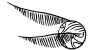
\includegraphics[scale=0.4]{boccino.png}
        \centering
\end{figure}

Una figura silenziosa scivolò sommessamente attraverso i freddi corridoi dei sotterranei di Hogwarts. Doveva essere presente in una certa stanza alle 18:00 per incontrare una certa persona, e se possibile era meglio arrivare prima, per mostrare rispetto.

Ma quando la sua mano girò la maniglia e aprì la porta di quell’aula buia, silenziosa, e inutilizzata, c’era già una sagoma lì in piedi, in mezzo alle file di vecchi banchi polverosi. Una sagoma che reggeva una piccola verga verde luminescente, la cui pallida luce illuminava con difficoltà persino colui che la reggeva, per non dire della stanza circostante.

La luce del corridoio morì appena la porta si chiuse dietro di lui, e gli occhi di Draco iniziarono il processo di adeguamento alla fioca luce.

La sagoma si voltò lentamente per osservarlo, rivelando un viso ombroso solo parzialmente illuminato dall’inquietante luce verde.

A Draco questo incontro piaceva già. Doveva mantenere la fredda luce verde, rendere entrambi più alti, fornire loro cappucci e maschere, spostarli da un’aula a un cimitero, e sarebbe stato identico all’inizio della metà delle storie che gli amici di suo padre raccontavano sui Mangiamorte.

«Voglio che tu sappia, Draco Malfoy», disse la sagoma nei toni di una calma mortale, «che non biasimo te per la mia recente sconfitta.»

Senza pensarci, Draco aprì la bocca per protestare, non vi era alcuna ragione plausibile per cui egli sarebbe dovuto essere biasimato –

«È stata dovuta, più che altro, alla mia stupidità», proseguì la figura indistinta. «Ci sono state molte altre cose che avrei potuto fare, a ciascun passo lungo la strada. Tu non mi hai chiesto di fare esattamente quello che ho fatto. Mi hai solo chiesto di aiutarti. Sono stato io a scegliere incautamente quel metodo in particolare. Ma resta il fatto che ho perso la gara per metà libro. Le azioni del tuo idiota addomesticato, e il favore che mi hai chiesto, e, sì, la mia stupidità nel soddisfarlo, mi hanno fatto perdere tempo. Più tempo di quanto tu non sappia. Tempo che, alla resa dei conti, si è rivelato decisivo. Resta il fatto, Draco Malfoy, che se non mi avessi chiesto quel favore, avrei vinto. E non… invece… perso.»

Draco aveva già sentito parlare della sconfitta di Harry e del pegno che Granger aveva riscosso. La notizia si era diffusa più velocemente di quanto i gufi avrebbero potuto fare.

«Comprendo», disse Draco. «Sono dispiaciuto.» Non c’era altro che potesse dire se voleva che Harry Potter gli fosse amico.

«Non chiedo comprensione o compassione», disse la sagoma oscura, ancora con quella calma mortale. «Ma ho appena trascorso due intere ore alla presenza di Hermione Granger, vestito con tali indumenti quali mi sono stati forniti, visitando luoghi di Hogwarts tanto affascinanti come una piccola cascata gorgogliante quello che mi è sembrato muco, accompagnato da un gruppo di altre ragazze che si sono ostinate in attività tanto utili quanto cospargere il nostro cammino con petali di rosa Trasfigurati. Sono stato a un appuntamento, rampollo dei Malfoy. Il mio primo appuntamento. E quando vorrò riscuotere quel favore, tu lo ripagherai.»

Draco annuì solennemente. Prima di arrivare aveva preso la saggia precauzione di informarsi su ogni dettaglio disponibile sull’appuntamento di Harry, in modo da esaurire tutte le proprie risate isteriche prima dell’ora stabilita per l’incontro, e non commettere un passo falso ridacchiando ininterrottamente fino a perdere conoscenza.

«Credi», disse Draco, «che dovrebbe accadere qualcosa di triste alla ragazza Granger –»

«Passa parola all’interno di Serpeverde che la ragazza Granger è mia e che chiunque si immischi nei miei affari avrà i suoi resti sparsi su una superficie sufficientemente vasta da coprire dodici diverse lingue parlate. E dal momento che io non sono in Grifondoro e uso l’astuzia piuttosto che gli attacchi frontali immediati, non dovranno farsi prendere dal panico se mi vedranno sorriderle.»

«O se dovessi essere visto a un secondo appuntamento?» chiese Draco, consentendosi appena una piccola nota di incredulità nella voce.

«Non ci sarà nessun secondo appuntamento», disse la sagoma illuminata di verde, con una voce così temibile che sembrò non solo simile a un Mangiamorte, ma ad Amycus Carrow quella volta, subito prima che suo Padre gli dicesse di smetterla, che non era il Signore Oscuro.

Naturalmente era ancora la voce acuta e bianca di un giovane ragazzo, e associata alle parole pronunciate, beh, semplicemente non era la stessa cosa. Se un giorno Harry Potter fosse diventato il prossimo Signore Oscuro, Draco avrebbe usato un Pensatoio per conservare una copia di questa memoria in un luogo sicuro, e Harry Potter non avrebbe mai osato tradirlo.

«Ma parliamo di cose più allegre», disse la figura ombreggiata di verde. «Parliamo di conoscenza e di potere. Draco Malfoy, parliamo di Scienza.»

«Sì», disse Draco. «Parliamo.»

Draco si chiese quanta parte del suo volto potesse essere vista, e quanta fosse in ombra, in quell’irreale luce verde.

E anche se Draco mantenne il suo volto serio, c’era un sorriso nel suo cuore.

Stava finalmente avendo una reale conversazione da adulto.

«Ti offro il potere», disse la figura in ombra, «e ti parlerò di quel potere e del suo prezzo. Il potere viene dal conoscere la forma della realtà e così facendo ottenere il controllo su di essa. Ciò che comprendi, puoi comandare, e questo è un potere sufficiente a camminare sulla Luna. Il prezzo di tale potere è che devi imparare a fare domande alla Natura e, cosa di gran lunga più difficile, accettare le risposte della Natura. Condurrai esperimenti, eseguirai prove e osserverai quello che accade. E dovrai accettare il significato di quei risultati quando ti dicono che stai sbagliando. Dovrai imparare a perdere, non contro di me, ma contro la Natura. Quando ti troverai a litigare con la realtà, dovrai lasciar vincere la realtà. Troverai tutto ciò doloroso, Draco Malfoy, e io non so se sei così forte. Conoscendone il prezzo, è ancora tuo desiderio imparare il potere umano?»

Draco fece un respiro profondo. Ci aveva riflettuto. Ed era difficile capire come potesse rispondere in altro modo. Aveva ricevuto l’istruzione di cogliere ogni opportunità di amicizia con Harry Potter. Si trattava semplicemente di imparare, non stava promettendo di fare nulla. Poteva sempre interrompere le lezioni in qualsiasi momento…

Certamente c’era un numero sufficiente di aspetti di questa situazione che la facevano sembrare una trappola, ma in tutta onestà, Draco non vedeva come tutto questo potesse andare storto.

Inoltre Draco aveva una certa voglia di conquistare il mondo.

«Sì», disse Draco.

«Eccellente», replicò la figura in ombra. «Ho avuto quel che si dice una settimana affollata, e ci vorrà tempo per pianificare il tuo piano di studi –»

«Ci sono molte cose che io stesso devo fare per consolidare il mio potere in Serpeverde», disse Draco, «per non parlare dei compiti. Forse dovremmo iniziare a ottobre?»

«Sembra ragionevole», disse la figura ombrosa, «ma quello che intendevo dire è che per pianificare il tuo piano di studi, ho bisogno di sapere che cosa ti insegnerò. Ho pensato a tre possibilità. La prima è che ti insegni la mente umana e il cervello. La seconda opzione è che ti insegni l’universo fisico, quelle arti che si trovano lungo la strada che porta alla Luna. Questo comporta una grande quantità di numeri, ma per un certo tipo di mente quei numeri sono più belli di ogni altra cosa la Scienza abbia da insegnare. Ti piacciono i numeri, Draco?»

Draco scosse la testa.

«Allora questo è determinato. Imparerai la matematica, prima o poi, ma non subito, credo. La terza opzione è che ti insegni la genetica e l’evoluzione e l’ereditarietà, ciò che potresti chiamare il sangue –»

«Questo», disse Draco.

La figura annuì. «Pensavo che avresti potuto rispondere così. Ma credo che sarà la strada più dolorosa per te, Draco. Che succede se la tua famiglia e gli amici, i puristi del sangue, dicono una cosa, e scoprissi che la prova sperimentale ne dice un’altra?»

«Allora scoprirò come far dare alla prova sperimentale la risposta giusta!»

Ci fu una pausa, come se la figura in ombra fosse rimasta lì, con la bocca aperta, per un breve periodo.

«Uhm», disse la figura ombrosa. «Non funziona proprio così. È da questo che stavo cercando di metterti in guardia, Draco. Non puoi far sì che la risposta sia qualunque cosa tu voglia.»

«Si può sempre far sì che la risposta sia quella che vuoi», disse Draco. Quella era stata praticamente la prima cosa che i suoi precettori gli avevano insegnato. «È solo una questione di trovare gli argomenti giusti.»

«No», disse la figura ammantata d’ombra, la voce che si alzò per la frustrazione, «no, no, no! Allora otterresti la risposta sbagliata e non puoi andare sulla Luna in questo modo! La Natura non è una persona, non puoi ingannarla e farle credere qualcosa di diverso, se cerchi di dire che la Luna che è fatta di formaggio puoi discutere per giorni e questo non cambierà la Luna! Ciò di cui stai parlando è la razionalizzazione, è come iniziare con un foglio di carta, andare direttamente all’ultima linea, scrivere ‘e quindi, la Luna è fatta di formaggio’, e poi tornar in cima per scriverci sopra ogni genere di argomentazione scaltra. Ma o la Luna è fatta di formaggio o non lo è. Nel momento in cui hai scritto l’ultima linea, era già vero o già falso. Che l’intero foglio di carta finisca per contenere la conclusione giusta o quella sbagliata si decide nell’istante in cui annoti l’ultima riga. Se stai cercando di scegliere tra due bauli costosi, e ti piace quello lucido, non importa quali argomenti intelligenti riesci a trovare per acquistarlo, la vera regola che hai usato per scegliere in favore di quale baule argomentare è stata ‘scegli quello lucido’, e otterrai un baule tanto buono quanto quella regola è in grado di scegliere. La razionalità non può essere usata per sostenere una posizione prefissata, il suo unico uso possibile è decidere da che parte schierarsi. Lo scopo della scienza non è convincere qualcuno che i puristi del sangue hanno ragione. Questa è politica! Il potere della scienza deriva dallo scoprire il modo in cui la Natura è realmente e che non può essere cambiato discutendo! Ciò che la scienza può fare è dirci come il sangue funziona realmente, come i maghi ereditano realmente i propri poteri dai loro genitori, e se i Nati babbani sono davvero più deboli o più forti –»

«Più forti!» sbottò Draco. Aveva cercato di seguire il ragionamento, un’espressione perplessa sul volto, e poteva capire come avesse una specie di senso ma certamente non era simile a nulla che avesse mai sentito prima. E poi Harry Potter aveva detto qualcosa che Draco non poteva lasciar passare. «Pensi che i Sanguemarcio siano più forti?»

«Non penso niente», disse la figura ombrosa. «Non so niente. Non credo in niente. La mia ultima riga non è stata ancora scritta. Scoprirò come mettere alla prova il potere magico dei Nati babbani, e il potere magico dei purosangue. Se le mie prove mi diranno che i Nati babbani sono più deboli, crederò che sono più deboli. Se le mie prove mi diranno che i Nati babbani sono più forti, crederò che sono più forti. Con la conoscenza di questa e altre verità, guadagnerò una certa quantità di potere –»

«E ti aspetti che io creda a qualunque cosa tu dica?» Draco domandò infervorato.

«Mi aspetto che tu esegua le prove personalmente», disse tranquillamente la figura in ombra. «Hai paura di ciò che tu scoprirai?»

Draco fissò la figura ammantata dall’ombra per un po’, con gli occhi socchiusi. «Bella trappola, Harry», disse. «Dovrò ricordarmela, è nuova.»

La figura ombrosa scosse la testa. «Non è una trappola, Draco. Ricorda — io non so cosa scopriremo. Ma non si comprende l’universo discutendo con lui o dicendogli di tornare con una risposta diversa la prossima volta. Quando indossi le vesti dello scienziato devi dimenticare tutta la tua politica e le discussioni e le fazioni e i partiti, mettere a tacere le posizioni disperatamente arroccate della tua mente, e desiderare solo di ascoltare la risposta della Natura.» La figura ombrosa fece una pausa. «La maggior parte delle persone non può farlo. Ecco perché è difficile. Sei sicuro che non vorresti piuttosto studiare il cervello?»

«E se ti dicessi che preferirei studiare il cervello», disse Draco, con la voce ora dura, «andresti in giro a dire alla gente che ho avuto paura di quello che avrei scoperto.»

«No», disse la figura ombrosa. «Non farei nulla del genere.»

«Ma potresti fare lo stesso tipo di prove da solo, e se ottenessi la risposta sbagliata, non sarei lì a dirti qualcosa prima che la mostrassi a qualcun altro.» La voce di Draco era ancora dura.

«Lo chiederei comunque prima a te, Draco», disse con calma la figura ombrosa.

Draco fece una pausa. Non se l’era aspettato, aveva pensato di aver visto la trappola, ma… «Lo faresti?»

«Certo. Come posso io sapere chi ricattare o cosa potremmo chiedere loro? Draco, ti ripeto ancora una volta che questa non è una trappola che ho creato per te. Almeno non per te personalmente. Se la tua posizione politica fosse stata diversa, ti starei chiedendo che cosa succederebbe se la prova mostrasse che i purosangue sono più forti.»

«Seriamente.»

«Sì! Questo è il prezzo che chiunque deve pagare per diventare uno scienziato!»

Draco alzò una mano. Doveva pensare.

La figura, ombrosa e illuminata di verde, attese.

Non ci volle molto tempo per pensarci, però. Se scartavi tutte le parti disorientanti… allora Harry Potter stava progettando di trafficare con qualcosa che avrebbe potuto provocare un gigantesco sconvolgimento politico, e sarebbe stato folle andarsene via e basta, e lasciare che facesse tutto da solo. «Studieremo il sangue», disse Draco.

«Eccellente», disse la figura, e sorrise. «Complimenti per essere disposto a fare la domanda.»

«Grazie», disse Draco, non riuscendo del tutto a escludere l’ironia dalla sua voce.

«Ehi, pensavi che andare sulla Luna fosse facile? Accontentati del fatto che richieda solo di cambiare idea qualche volta, e non un sacrificio umano!»

«Il sacrificio umano sarebbe molto più facile!»

Ci fu una breve pausa, e poi la figura annuì. «Giusta osservazione.»

«Ascolta, Harry», disse Draco senza molte speranze, «pensavo che l’idea fosse di prendere tutte le cose che i Babbani sanno, combinarle con le cose che i maghi sanno, e diventare padroni di entrambi i mondi. Non sarebbe molto più facile studiare tutte le cose che i Babbani hanno già scoperto, come la roba della Luna, e usare quel potere –»

«No», disse la figura scuotendo decisamente la testa, ombre verdi che si mossero intorno al naso e agli occhi. La sua voce era diventata molto triste. «Se non puoi imparare l’arte dello scienziato di accettare la realtà, allora non devo dirti cosa quell’accettazione ha portato a scoprire. Sarebbe come se un potente mago ti svelasse le porte che non devono essere aperte e i sigilli che non devono essere spezzati, prima che tu abbia dimostrato di possedere l’intelligenza e la disciplina necessarie per sopravvivere ai pericoli minori.»

Un brivido scese lungo la schiena di Draco, che tremò involontariamente. Sapeva che era stato visibile anche nella penombra. «Va bene», disse Draco. «Comprendo.» Suo Padre gliel’aveva detto molte volte. Quando un mago più potente ti diceva che non eri pronto a sapere, non dovevi curiosare oltre, se volevi vivere.

La figura chinò il capo. «Già. Ma c’è un’altra cosa che dovresti comprendere. I primi scienziati, essendo Babbani, non avevano le vostre tradizioni. In principio, semplicemente non compresero il concetto di conoscenza pericolosa, e pensarono che di tutte le cose conosciute si dovesse parlare liberamente. Quando le loro ricerche divennero pericolose, riferirono ai loro politici cose che sarebbero dovute restare segrete — non guardarmi così, Draco, non fu semplicemente stupidità. Dovevano essere abbastanza intelligenti da scoprire quei segreti, del resto. Ma erano Babbani, era la prima volta che avevano trovato qualcosa di veramente pericoloso, e non erano stati iniziati a una tradizione di segretezza. C’era una guerra in corso, e gli scienziati di una parte erano preoccupati che se loro non avessero parlato, gli scienziati del paese nemico l’avrebbero detto per primi ai loro politici…» La frase rimase sospesa in modo significativo. «Non distrussero il mondo. Ma ci andarono vicino. E noi non abbiamo intenzione di ripetere lo stesso errore.»

«Giusto», disse Draco, la voce ora molto ferma. «Noi non lo faremo. Noi siamo maghi, e studiare la scienza non ci rende Babbani.»

«È come dici», riprese la sagoma illuminata di verde. «Creeremo la nostra Scienza, una Scienza magica, e questa Scienza possiederà tradizioni più intelligenti fin dal principio.» La voce si fece dura. «La conoscenza che condivido con te sarà insegnata insieme alle discipline per accettare la verità, il livello di questa conoscenza sarà vincolato ai tuoi progressi in quelle discipline, e non condividerai tale conoscenza con nessun altro che non abbia imparato quelle discipline. Accetti queste condizioni?»

«Sì», disse Draco. Cosa ci si aspettava da lui, che dicesse no?

«Bene. E quello che scoprirai tu stesso, lo terrai per te a meno che non riterrai che altri scienziati siano pronti a conoscerlo. Ciò che condivideremo tra di noi, non lo riveleremo al mondo se non saremo d’accordo che sia sicuro per il mondo saperlo. E qualunque siano le nostre relazioni politiche e chiunque sia a godere della nostra lealtà, tutti noi puniremo chiunque nel nostro gruppo riveli magie o armi pericolose, non importa che tipo di guerra sia in corso. Da questo giorno in poi, questa sarà la tradizione e la legge della scienza tra i maghi. Siamo d’accordo su questo?»

«Sì», disse Draco. In verità tutto questo cominciava a sembrare piuttosto interessante. I Mangiamorte avevano tentato di prendere il potere facendo in modo di essere più terrificanti di chiunque altro, e in realtà non avevano ancora vinto. Forse era il momento di provare a governare usando i segreti, piuttosto. «E il nostro gruppo rimane nascosto il più a lungo possibile, e tutti al suo interno devono accettare le nostre regole.»

«Naturalmente. Assolutamente.»

Ci fu una breve pausa.

«Avremo bisogno di vesti migliori», disse la figura ombrosa, «con cappucci e cose simili –»

«Ci stavo proprio pensando», disse Draco. «Non abbiamo bisogno di vesti completamente nuove, però, solo mantelli a cappuccio da indossarci sopra. Ho un’amica Serpeverde, prenderà le tue misure –»

«Non dirle a cosa serve, però –»

«Non sono stupido!»

«E niente maschere per ora, non quando siamo solo tu e io –» disse la figura ombrosa.

«Giusto! Ma in seguito dovremmo trovare una sorta di marchio speciale che tutti i nostri servitori avranno, il Marchio della Scienza, come un serpente che mangia la Luna sul braccio destro –»

«Si chiama dottorato di ricerca e non renderebbe troppo facile identificare i nostri?»

«Eh?»

«Voglio dire, che succederebbe se qualcuno dicesse ‘ok, ora sollevate tutti le vostre vesti sul braccio destro’ e il nostro uomo rispondesse ‘oops, scusate, sembra che io sia una spia’ –»

«Dimentica quello che ho detto», disse Draco, il sudore diffusosi improvvisamente per tutto il corpo. Aveva bisogno di un diversivo, velocemente — «E come ci chiameremo? I Mangiascienza?»

«No», disse lentamente la figura ombrosa. «Non suona bene…»

Draco si asciugò la fronte col braccio, rimuovendo le gocce di sudore. Cosa aveva pensato il Signore Oscuro? Suo Padre aveva detto che il Signore Oscuro era intelligente!

«Ce l’ho!» disse improvvisamente la figura ombrosa. «Non lo capirai ora, ma fidati, è adatto.»

In quel momento Draco avrebbe accettato anche ‘Masticatori di Malfoy’, purché si cambiasse argomento. «Che cos’è?»

E in piedi in mezzo ai banchi polverosi in un’aula inutilizzata nei sotterranei di Hogwarts, la sagoma illuminata di verde di Harry Potter allargò platealmente le braccia e disse: «Questo giorno segnerà l’alba della… Cospirazione bayesiana.»

\begin{figure}[h!]
        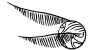
\includegraphics[scale=0.4]{boccino.png}
        \centering
\end{figure}

Una figura silenziosa si trascinò stancamente per i corridoi di Hogwarts in direzione di Corvonero.

Harry era andato direttamente dall’incontro con Draco a cena, e ci era rimasto per un tempo a malapena sufficiente a trangugiare un paio di bocconi veloci prima di andare a letto.

Non erano neppure le 19, ancora, ma era ben oltre l’ora di coricarsi per Harry. Si era reso conto ieri sera che sabato non sarebbe stato in grado di utilizzare il Giratempo fino a dopo la fine della gara di lettura. Ma poteva ancora usare il Giratempo venerdì sera, e guadagnare tempo in questo modo. Così Harry si era sforzato di restare sveglio venerdì fino alle 21, quando il guscio protettivo si era aperto, e poi aveva utilizzato le quattro ore restanti sul Giratempo per tornare alle 17 e collassare dal sonno. Si era svegliato intorno alle 2 di sabato mattina, come previsto, e aveva letto per le successive dodici ore di fila… e ancora non era stato sufficiente. E ora Harry sarebbe andato a dormire piuttosto presto per i prossimi giorni, fino a quando il suo ciclo di sonno non si fosse nuovamente riallineato.

Il ritratto sulla porta chiese a Harry qualche sciocco enigma pensato per bambini di undici anni, che risolse senza che le parole passassero attraverso la sua mente cosciente, e poi Harry barcollò su per le scale fino alla sua stanza del dormitorio, si mise il pigiama e crollò sul letto.

E trovò che il suo cuscino sembrava piuttosto bitorzoluto.

Harry gemette. Si sedette con riluttanza, si contorse nel letto, e sollevò il cuscino.

Questo rivelò una nota, due galeoni d’oro, e un libro intitolato Occlumanzia: l’Arte Nascosta.

Harry prese la nota e lesse:

Accidenti, ti metti davvero nei guai, e in fretta. Tuo padre non era al tuo livello.

Ti sei fatto un nemico potente. Snape gode della lealtà, dell’ammirazione e della paura di tutti a Casa Serpeverde. Non puoi fidarti di chiunque appartenga a quella Casa ora, che venga a te in veste amichevole o tremenda.

D’ora in poi non devi fissare gli occhi di Snape. È un Legilimens e sarebbe in grado di leggere la tua mente se lo facessi. Ho incluso un libro che potrebbe aiutarti a imparare a proteggerti, anche se senza un precettore c’è un limite a quanto puoi ottenere. Ad ogni modo puoi sperare quanto meno di accorgerti delle intrusioni.

Affinché tu possa trovare un po’ di tempo in più in cui studiare Occlumanzia, ho allegato due galeoni, che sono il prezzo delle soluzioni degli esami e dei compiti a casa per il primo anno del corso di Storia della Magia (da quando è morto il professor Binns ha dato gli stessi esami e gli stessi compiti ogni anno). I tuoi nuovi amici, i gemelli Weasley, dovrebbero essere in grado di venderti una copia. Va da sé che è necessario non farti prendere con essi in tuo possesso.

Del professor Quirrell so poco. È un Serpeverde e un professore di Difesa, e questi sono due indizi contro di lui. Considera attentamente ogni consiglio che ti dà, e non dirgli nulla che non desideri sia reso noto.

Silente fa solo finta di essere pazzo. È molto intelligente, e se continui a entrare nei ripostigli e a svanire, certamente dedurrà il tuo possesso di un mantello dell’invisibilità, se non l’ha già fatto. Evitalo quando possibile, nascondi il Mantello dell’Invisibilità in qualche posto sicuro (non la tua borsa) ogni volta che non puoi evitarlo, e agisci con gran circospezione in sua presenza.

Per favore, stai più attento in futuro, Harry Potter.

–- Babbo Natale

Harry fissò la nota.

E sembrava essere un ottimo consiglio. Certo Harry non aveva intenzione di imbrogliare nel corso di Storia, anche se gli avessero dato una scimmia morta come professore. Ma la Legilimanzia di Severus… chiunque avesse inviato questa nota sapeva parecchi segreti importanti ed era disposto a raccontarli a Harry. La nota lo stava ancora mettendo in guardia contro la possibilità che Silente rubasse il mantello, ma a questo punto onestamente Harry non aveva idea se fosse un brutto segno, sarebbe potuto essere solo un errore comprensibile.

Pareva che ci fosse una sorta di intrigo in atto all’interno di Hogwarts. Forse se Harry avesse confrontato le storie tra Silente e il mittente della nota, avrebbe potuto tirare fuori un quadro combinato che sarebbe stato accurato? Del tipo se entrambi fossero stati d’accordo su qualcosa, allora…

… evabbè…

Harry ficcò tutto nella borsa, alzò il Quietus, tirò la coperta sopra la testa e si spense.

\begin{figure}[h!]
        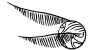
\includegraphics[scale=0.4]{boccino.png}
        \centering
\end{figure}

Era domenica mattina e Harry stava mangiando frittelle nella Sala Grande, con piccoli morsi frequenti, gettando occhiate nervose al suo orologio ogni pochi secondi.

Erano le 8:02, e tra due ore e un minuto precisi sarebbe stata esattamente una settimana da quando aveva visto i Weasley e attraversato il varco verso il Binario Nove e Tre Quarti.

E gli venne un pensiero… Harry non sapeva se questo fosse un modo valido di pensare riguardo all’universo, non sapeva più nulla, ma sembrava possibile…

Che…

Non gli fossero successe abbastanza cose interessanti durante la settimana passata.

Per quando ebbe finito di fare colazione, Harry aveva deciso di andare dritto in camera sua e nascondersi nel livello inferiore del suo baule e non parlare con nessuno fino alle 10:03.

E fu allora che Harry vide i gemelli Weasley camminare verso di lui. Uno di loro portava qualcosa nascosto dietro la schiena.

Avrebbe dovuto scappare urlando.

Avrebbe dovuto scappare urlando.

Di qualunque cosa si trattasse… poteva benissimo essere…

… il gran finale…

Avrebbe davvero dovuto scappare urlando.

Con la rassegnazione che l’universo sarebbe venuto a prenderlo comunque, Harry continuò a tagliare la frittella con la forchetta e il coltello. Non riusciva a chiamare a raccolta le proprie forze. Quella era la triste verità. Harry sapeva ormai come le persone si sentivano quando erano stanche di correre, stanche di cercare di sfuggire al destino, e cadevano semplicemente a terra e lasciavano che i demoni orribilmente artigliati e tentacolati del più oscuro abisso le trascinassero via verso il loro indicibile destino.

I gemelli Weasley si avvicinarono.

E furono ancora più vicini.

Harry mangiò un altro boccone di frittella.

I gemelli Weasley arrivarono, sorridendo allegramente.

«Ciao, Fred», disse Harry debolmente. Uno dei gemelli annuì. «Ciao, George.» L’altro gemello annuì.

«Sembri stanco», disse George.

«Dovresti rallegrarti», disse Fred.

«Guarda che cosa ti abbiamo portato noi!»

E George prese, da dietro le spalle di Fred –

Una torta con dodici candeline fiammeggianti.

Ci fu una pausa, mentre il tavolo di Corvonero li fissò.

«Vi sbagliate», disse qualcuno. «Harry Potter è nato il trentuno lugl-»

«egli sta arrivando», disse un’alta voce cavernosa che passò attraverso tutte le conversazioni come una spada di ghiaccio. «colui che distruggerà persino –»

Silente era saltato fuori dal suo trono ed era corso dritto oltre il Tavolo d’onore e aveva afferrato la donna che pronunciava quelle parole terribili, Fawkes era apparso in un lampo e tutti e tre erano scomparsi in uno schiocco di fuoco.

Ci fu una pausa traumatizzata…

… seguita dal movimento delle teste che si voltarono in direzione di Harry Potter.

«Non sono stato io», disse Harry con voce stanca.

«Quella era una profezia!» sibilò qualcuno al tavolo. «E scommetto che riguarda te!»

Harry sospirò.

Si alzò dal suo posto, schiarì la voce, e disse a voce alta al di sopra delle conversazioni che stavano nascendo, «Non si tratta di me! È ovvio! Io non sto venendo qui, io sono già qui!»

Harry tornò nuovamente a sedersi.

Le persone che erano state a guardarlo si girarono di nuovo.

Qualcun altro al tavolo chiese «Allora di chi si tratta?»

E con una sorda e plumbea sensazione, Harry si rese conto di chi non era già a Hogwarts.

Chiamatelo tirare a indovinare, ma Harry aveva la sensazione che il non-morto Signore Oscuro sarebbe comparso uno di quei giorni.

La conversazione proseguì intorno a lui.

«E poi, distruggere cosa?»

«Mi pare che Trelawney stesse per dire qualcosa che iniziava per ‘s’, poco prima che il Preside l’afferrasse».

«Come… spirito? Sole?»

«Se qualcuno sta per distruggere il Sole siamo davvero nei guai!»

Sembrava piuttosto improbabile a Harry, a meno che il mondo non contenesse cose spaventose che avevano sentito parlare delle idee di David Criswell circa l’aspirazione delle stelle.

«E così», disse Harry in tono stanco, «cose come queste succedono ogni domenica a colazione, vero?»

«No», disse uno studente che avrebbe potuto essere al settimo anno, accigliato e torvo. «Non succedono.»

Harry scrollò le spalle. «Pazienza. Qualcuno vuole un po’ di torta di compleanno?»

«Ma non è il tuo compleanno!» disse lo stesso studente che aveva obiettato in precedenza.

Quello fu lo spunto per Fred e George per iniziare a ridere, naturalmente.

Anche Harry riuscì a fare un sorriso stanco.

Mentre gli veniva servita la prima fetta, Harry disse: «Ho avuto una settimana molto lunga.»

\begin{figure}[h!]
        \includegraphics[scale=0.4]{boccino.png}
        \centering
\end{figure}

E Harry era seduto nel livello sotterraneo del suo baule, chiuso a chiave in modo che nessuno potesse entrare, una coperta tirata sulla testa, in attesa che la settimana fosse finita.

10:01.

10:02.

10:03, ma giusto per essere sicuri…

10:04 e la prima settimana era andata.

Harry tirò un sospiro di sollievo, e cautamente tolse la coperta dalla testa.

Pochi istanti dopo, era emerso nell’aria del suo dormitorio illuminato vividamente dal sole.

Ancora poco, e fu nella sala comune di Corvonero. Alcune persone lo guardarono, ma nessuno disse niente o cercò di parlargli.

Harry trovò una bella e ampia scrivania, avvicinò una comoda sedia, e si sedette. Dalla sua borsa estrasse un foglio di carta e una matita.

Mamma e papà avevano detto a Harry senza mezzi termini che, sebbene avrebbero capito il suo entusiasmo di allontanarsi da casa e dai suoi genitori, avrebbe dovuto scrivere loro ogni settimana senza fallo, giusto in modo che sapessero che era vivo, illeso, e ancora a piede libero.

Harry fissò il foglio di carta bianco. Vediamo…

Dopo aver lasciato i suoi genitori alla stazione ferroviaria, aveva…

… fatto conoscenza con un ragazzo cresciuto da Darth Vader, fatto amicizia con i tre burloni più famigerati di Hogwarts, incontrato Hermione, e poi c’era stato l’incidente con il Cappello Smistatore… lunedì aveva ricevuto una macchina del tempo per curare il suo disturbo del sonno, ricevuto un leggendario mantello dell’invisibilità da un benefattore sconosciuto, salvato sette Tassofrasso fissando cinque spaventosi ragazzi più grandi uno dei quali aveva minacciato di rompergli il dito, compreso che possedeva un misterioso lato oscuro, imparato a lanciare Frigideiro nella lezione di Incantesimi, e iniziato la sua rivalità con Hermione… martedì aveva fatto conoscenza con Astronomia insegnata dalla professoressa Aurora Sinistra, che era interessante, e con Storia della Magia insegnata da un fantasma che avrebbe dovuto essere esorcizzato e sostituito con un registratore… mercoledì, era stato dichiarato lo Studente Più Pericoloso della Classe… giovedì, meglio non pensarci nemmeno a giovedì… venerdì, l’incidente della lezione di Pozioni, seguito dal suo ricatto al Preside, seguito dal Professore di Difesa che l’aveva fatto picchiare a lezione, seguito dal Professore di Difesa che si era rivelato l’essere umano più fantastico che camminasse sulla faccia della Terra… sabato aveva perso una scommessa ed era andato al suo primo appuntamento e aveva iniziato la redenzione di Draco… e poi quella mattina la profezia incompleta della professoressa Trelawney che poteva o non poteva indicare che un Signore Oscuro immortale stava per attaccare Hogwarts.

Harry organizzò mentalmente il materiale, e iniziò a scrivere.

Cari Mamma e Papà,

Hogwarts è molto divertente. Ho imparato a violare la Seconda Legge della Termodinamica alla lezione di Incantesimi, e ho incontrato una ragazza di nome Hermione Granger che legge più velocemente di me.

Sarà meglio che mi fermi qui.

Vostro figlio che vi ama tanto,

Harry James Potter-Evans-Verres.





%\appendix

%\input{Appendix.tex}

%% bibliography, analytical index etc...
\backmatter

%\summary
%\begin{figure}[h]
%    \centering
%    \includegraphics[width=1\textwidth]{paper.png}
%    \caption{so... yeah... this paper is really about...uh...}
%    \label{fig:Hope it doesn't happen...}
%\end{figure}


\newpage
\bibliographystyle{plain_\languagename}
%% recommended

% xkcd as bibliography title
%\renewcommand{\chapter}[2]{
%\begin{figure}[h]
%    \centering
%    \includegraphics[width=0.5\textwidth]{xkcd/citogenesis.png}
%    \caption*{[xkcd.org]}
%    \label{fig:So standard}
%\end{figure}}
%\bibliography{thud}
%% use `thebibliography' environment for manual bibliography

%\printindex

\end{document}
